\documentclass[openany,fontset=none]{ctexbook}
%=================  北京大学计算机基础能力手册  =================%
%                          preamble.tex                          %
%================================================================%

%---------- 常用宏包 ----------
\usepackage{geometry}
\geometry{b5paper, margin=0.5in}
\usepackage{amssymb,amsmath}
\usepackage{fontspec}
\usepackage{xeCJK}
\usepackage{graphicx}
\graphicspath{{./images/}}
\usepackage{longtable,array,booktabs}
\usepackage{multicol}
\usepackage{subcaption}
\usepackage{enumitem}
\usepackage{listings}
\usepackage[table]{xcolor}
\usepackage{tcolorbox}
\tcbuselibrary{skins,xparse,most,breakable}
\usepackage{manyfoot,perpage}
\usepackage{url}
\usepackage{hyperref}
\usepackage{fontawesome5}
\usepackage{authblk}

%---------- 页面与字体 ----------
\setmainfont{Source Serif Pro Light}
\setsansfont{Source Sans Pro Light}
\setmonofont{Source Code Pro Light}
\setCJKmainfont[ItalicFont=Source Han Serif CN]{Source Han Serif CN}
\setCJKsansfont{Source Han Sans CN}
\setCJKmonofont{Source Han Sans CN}

%---------- 列表、代码、脚注 ----------
\setlist{nosep}
\lstset{
  basicstyle=\ttfamily\footnotesize,
  keywordstyle=\color{blue},
  commentstyle=\color{green!50!black},
  stringstyle=\color{red},
  numbers=left,numberstyle=\tiny\color{gray},stepnumber=1,numbersep=5pt,
  backgroundcolor=\color{white},
  showspaces=false,showstringspaces=false,breaklines=true,frame=single
}

\DeclareNewFootnote{B}[roman]
\renewcommand{\thefootnoteB}{}          % 无编号
\makeatletter
\let\fnB@mark\relax                      % 不输出标记
% 重新定义 \href:正文蓝色下划线 + 外部箭头 + 底部脚注
\let\oldhref\href
\renewcommand{\href}[2]{%
  \oldhref{#1}{\color{blue}\underline{#2}\raisebox{0.2ex}{\tiny$\nearrow$}}%
  \footnotetextB{\textbf{#2}: \url{#1}}%
}
\makeatother

\hypersetup{colorlinks=false,pdfborder={0 0 0}}

%---------- tcolorbox 环境 ----------
\newtcolorbox{warning}{enhanced,colback=red!4!white,colframe=red!75!black,coltitle=white,fonttitle=\bfseries,title=警告,top=2mm,bottom=2mm,left=2.5mm,right=2.5mm,boxrule=0.6pt,breakable}
\newtcolorbox{caution}{enhanced,colback=orange!5!white,colframe=orange!60!black,coltitle=white,fonttitle=\bfseries,title=注意,top=2mm,bottom=2mm,left=2.5mm,right=2.5mm,boxrule=0.6pt,breakable}
\newtcolorbox{tip}{enhanced,colback=cyan!3!white,colframe=cyan!65!black,coltitle=white,fonttitle=\bfseries,title=提示,top=2mm,bottom=2mm,left=2.5mm,right=2.5mm,boxrule=0.6pt,breakable}
\newtcolorbox{note}{enhanced,colback=teal!3!white,colframe=teal!60!black,coltitle=white,fonttitle=\bfseries,title=说明,top=2mm,bottom=2mm,left=2.5mm,right=2.5mm,boxrule=0.6pt,breakable}
\newtcolorbox{example}[1][]{enhanced,colback=blue!3!white,colframe=blue!70!black,coltitle=white,fonttitle=\bfseries,title={\IfBlankTF{#1}{例题}{例题 (#1)}},top=2mm,bottom=2mm,left=2.5mm,right=2.5mm,boxrule=0.6pt,breakable}
\newtcolorbox{answer}{enhanced,colback=green!4!white,colframe=green!65!black,coltitle=white,fonttitle=\bfseries,title=答案,top=2mm,bottom=2mm,left=2.5mm,right=2.5mm,boxrule=0.6pt,breakable}
\newtcolorbox{exercise}{enhanced,colback=violet!4!white,colframe=violet!70!black,coltitle=white,fonttitle=\bfseries,title=练习,top=2mm,bottom=2mm,left=2.5mm,right=2.5mm,boxrule=0.6pt,breakable}
\newtcolorbox{thinking}{enhanced,colback=yellow!4!white,colframe=yellow!70!black,coltitle=white,fonttitle=\bfseries,title=开放性思考和探索,top=2mm,bottom=2mm,left=2.5mm,right=2.5mm,boxrule=0.6pt,breakable}

%---------- 标题信息 ----------
\title{\Huge\textbf{北京大学计算机基础能力手册}}
\author[1]{臧炫懿}
\affil[1]{北京大学学生Linux俱乐部}
\affil[ ]{\faGithub\ \texttt{ZangXuanyi/getting-started-handout}}
\affil[ ]{\faEnvelope\ \texttt{zangxuanyi@stu.pku.edu.cn}}
\renewcommand*{\Authsep}{, }
\renewcommand*{\Authand}{, }
\renewcommand*{\Authands}{, }
\date{}

% \includeonly{chapters/204-pragmatic-coding}

\begin{document}
\maketitle
\frontmatter
\chapter{前言}

计算机基础科学教育是我国近些年一直努力推进的教育之一,北京大学的所有学生都应修习《计算概论》课程。然而,大学计算机基础教育的内容往往过于理论化,缺乏实用性,这使得同学们在学习过程中容易感到枯燥乏味,在学习之后也很难将所学知识灵活应用到实际生产与生活中,最终导致在校学生对计算机的使用和开发能力普遍较低,甚至出现了“念了四年本科却不会用Git”的现象。同时,我国初高中乃至小学阶段,计算机的教育水平参差不齐,同学们的基础也不尽相同,这导致部分基础较差的同学在学习《计算概论》时会遇到困难,遑论进阶课程。

在本手册正式编写之前,已经有很多学长为了抹平基础知识的差距做出了相关的努力。几个广为人知的项目:北京大学为新生提供了《计算概论衔接课》,旨在帮助同学们快速入门计算机基础知识(这门课的前半部分由我所讲授);北京大学学生Linux俱乐部(LCPU)启动了\href{missing.lcpu.dev}{Getting Started项目},旨在帮助同学们快速入门Linux和计算机科学(该项目亦由我全权负责);一位\faGithub\href{https://github.com/PKUFlyingPig}{学长}发起了\href{https://csdiy.wiki/}{CS自学指南}项目,受到了广泛的关注和认可,该项目迄今已有一百五十余位贡献者;PKUHub等其他官方或非官方的组织也在积极推动计算机基础教育的普及。

然而,Getting Started和自学指南对于大一新生而言,存在的最大不足之处就是:不够基础。而对于有能力就读北大的学生而言,“上课”这种获取信息的形式的信息密度显然是不够的,大约是已经不再幻想上课有用了;真正有用的知识还是要靠同学们自己去学习实践。因此,我认为给同学们一本手册要比给同学们数小时的课程视频有用得多。笔者最终决定:制作这份手册,帮助同学们把初高中缺失的计算机知识,以及大学丢失的开发能力补回来。

本手册可以认为是对大学常用计算机基础知识与基础开发能力的汇总,比起深度更注重广度,比起理论更注重实践。简而言之,我们手册中会讲一些\textbf{正课几乎不会讲、但是用处极大}的知识。我们认为使用本手册的同学都已经具备了最基本的计算机操作能力,例如“使用鼠标”“关机”这种操作默认大家非常熟练,因此也不会涉及相关内容。

本手册正文分为两部分。第一部分面向计算机新手,讲述计算机基础知识,内容涵盖计算机组成和使用、编程环境配置、文本处理、Linux等内容,旨在将同学们的水平提升至能够接受大学计算机基础教育的水平;第二部分则面向工程开发新手,讲述工程开发的一些基础内容,包含C++和Python的语法基础、实用主义编程、调试和C语言工具链等,旨在将同学们的水平提升至能够进行简单工程开发的水平。

本文偏理论的章节中有一些“开放性思考和探索”板块,使用黄色背景色标注,旨在引导同学们进行更深入的思考和探索。笔者仅仅提供一些选题供参考,自己也不知道有没有一个确定的答案以及答案是什么,因此也不会给出答案甚至思路。有兴趣、有技术的同学们可以自行探索相关话题,甚至可以作为大作业、数学建模、科创甚至毕业设计的选题种子。当然,如果觉得难度过高,也完全可以跳过。

本手册以本人实践和经验为基底讲授。\textbf{如果本手册中的内容和正课中的内容或要求有差异,请以正课为准。}

本手册参考了LCPU Getting Started以及诸多博文、指南的内容,并在此基础上进行了增删和修改。

希望本手册能够对同学们有所帮助。

如有疑问、意见或建议,欢迎来该项目的仓库\faGithub\href{https://github.com/ZangXuanyi/getting-started-handout}{ZangXuanyi/getting-started-handout}查看本手册的源代码,欢迎提出Issue与Pull Request。如不能访问,也可向我发送电子邮件咨询:\texttt{zangxuanyi@stu.pku.edu.cn}。

\begin{figure}[ht]
  \centering
  
\includegraphics[width=0.5\textwidth]{000/fly.jpg}
\end{figure}

\mainmatter
\tableofcontents

\part{打好基础}
\chapter{初步认识计算机}

在真正学习计算机的有关内容之前,我们需要对计算机有一个最初步的认识。计算机是一个复杂的系统,它由许多不同的部件和组件组成,这些部件和组件共同工作以完成各种任务。

\section{计算机的发展历史}

人们一直在思考怎样进行更高效的计算。在古代,算盘、算筹等工具被用来进行计算。后来,随着科学技术的发展,人们对计算的需求越来越高,开始设计和制造更复杂的计算设备。查尔斯·巴贝奇(Charles Babbage)被认为是计算机的鼻祖,他在19世纪设计了第一台机械计算机——差分机和分析机。虽然他的设计在当时没有被完全实现,但他的思想为后来的计算机发展奠定了重要的基础。后来,也出现了一些其他的机械或电子计算设备,例如赫尔曼·霍列里斯(Herman Hollerith)发明的打孔卡机,该机器用于处理美国人口普查数据。

我们一般认为,阿兰·图灵(Alan Turing)是赋予现代计算机灵魂的人。他在1936年提出了“图灵机”的概念,图灵机是一个抽象的计算模型,能够模拟任何计算机的计算过程。自此,问题被分为两类:能用图灵机解决的(或者称作“图灵可计算的”)和不能用图灵机解决的;遇到前者,我们就可以掏出图灵机计算。图灵机的提出为现代计算机科学奠定了基础。

然而,图灵机更多的是一种抽象概念,真正把计算机变成现实的是冯·诺依曼。冯·诺依曼在1945年总结前人经验,提出并推广了“普林斯顿架构”。后来这个架构也被称作“冯·诺依曼架构”,也就是我们现在所说的计算机的基本结构。冯·诺依曼架构的核心思想是将程序和数据存储在同一块内存中,这样计算机就可以根据程序的指令来操作数据。冯·诺依曼架构是现代计算机的基础,目前几乎所有的计算机都遵循这一架构。

第一台真正意义上的电子计算机是ENIAC(Electronic Numerical Integrator and Computer),它于1946年由约翰·莫克利(John Mauchly)和约翰·普雷斯珀·埃克特(J. Presper Eckert)设计和建造。ENIAC使用了电子管作为主要的计算元件,计算速度可达每秒5000次加法运算。ENIAC的出现标志着电子计算机时代的到来——虽然它一开始是十进制的,实际上也并没有采用冯·诺依曼架构;直到1947年之后才被部分改造,引入了类似冯·诺依曼架构的设计。

随着技术的不断进步,计算机经历了多次重大变革。1950年代,晶体管的发明使得计算机变得更小、更快、更可靠、更节能。1960年代,集成电路(IC)的出现进一步推动了计算机的发展,使得计算机的性能大幅提升。1970年代,微处理器(SoC)的出现使得个人计算机成为可能。1980年代,图形用户界面(GUI)的引入使得计算机更加易于使用。1990年代,互联网的兴起使得计算机成为全球信息交流的重要工具,计算机也因为SoC真正得到广泛应用而开始走进千家万户。计算机的计算能力也早已今非昔比,如今一台家用计算机的计算能力已经达到每秒数十亿次浮点运算(GFLOPS),而高端服务器和超级计算机的计算能力更是达到了每秒数万亿次浮点运算(TFLOPS)甚至更高。

时至今日,计算机已经成为我们生活中不可或缺的一部分。无论是在工作、学习还是娱乐中,计算机都发挥着重要的作用。随着人工智能、大数据、云计算等新技术的不断涌现,计算机的未来发展充满了无限可能。

非常有趣的是,ENIAC的“生日”正是1946年2月14日,也就是情人节。或许这也象征着计算机与人类之间的深厚情感纽带。

\section{现代计算机的组成}

计算机的组成可以分为\textbf{硬件}和\textbf{软件}两大部分。硬件是指计算机的物理部件,如中央处理器(CPU)、内存、硬盘、显示器等;软件是指计算机上运行的程序和操作系统,如Windows、Linux、macOS等操作系统,以及Google Chrome、Microsoft VS Code、Tencent QQ等应用程序。

\subsection{计算机的硬件}

计算机的\textbf{硬件},也可以叫做\textbf{设备},可以简单分为两类:一类叫做\textbf{主机设备},是计算机用来进行计算等工作的设备;另一类叫做\textbf{外设设备}(也可以叫做\textbf{输入输出设备}),是计算机与外界进行信息交互的设备。通常说来,前者是藏在机箱里看不见的,后者是我们能够直接看见的。

一个计算机的主机设备如图\ref{fig:computer-hardware}所示。下面将会逐个介绍这些设备。
\begin{figure}[ht]
  \centering
  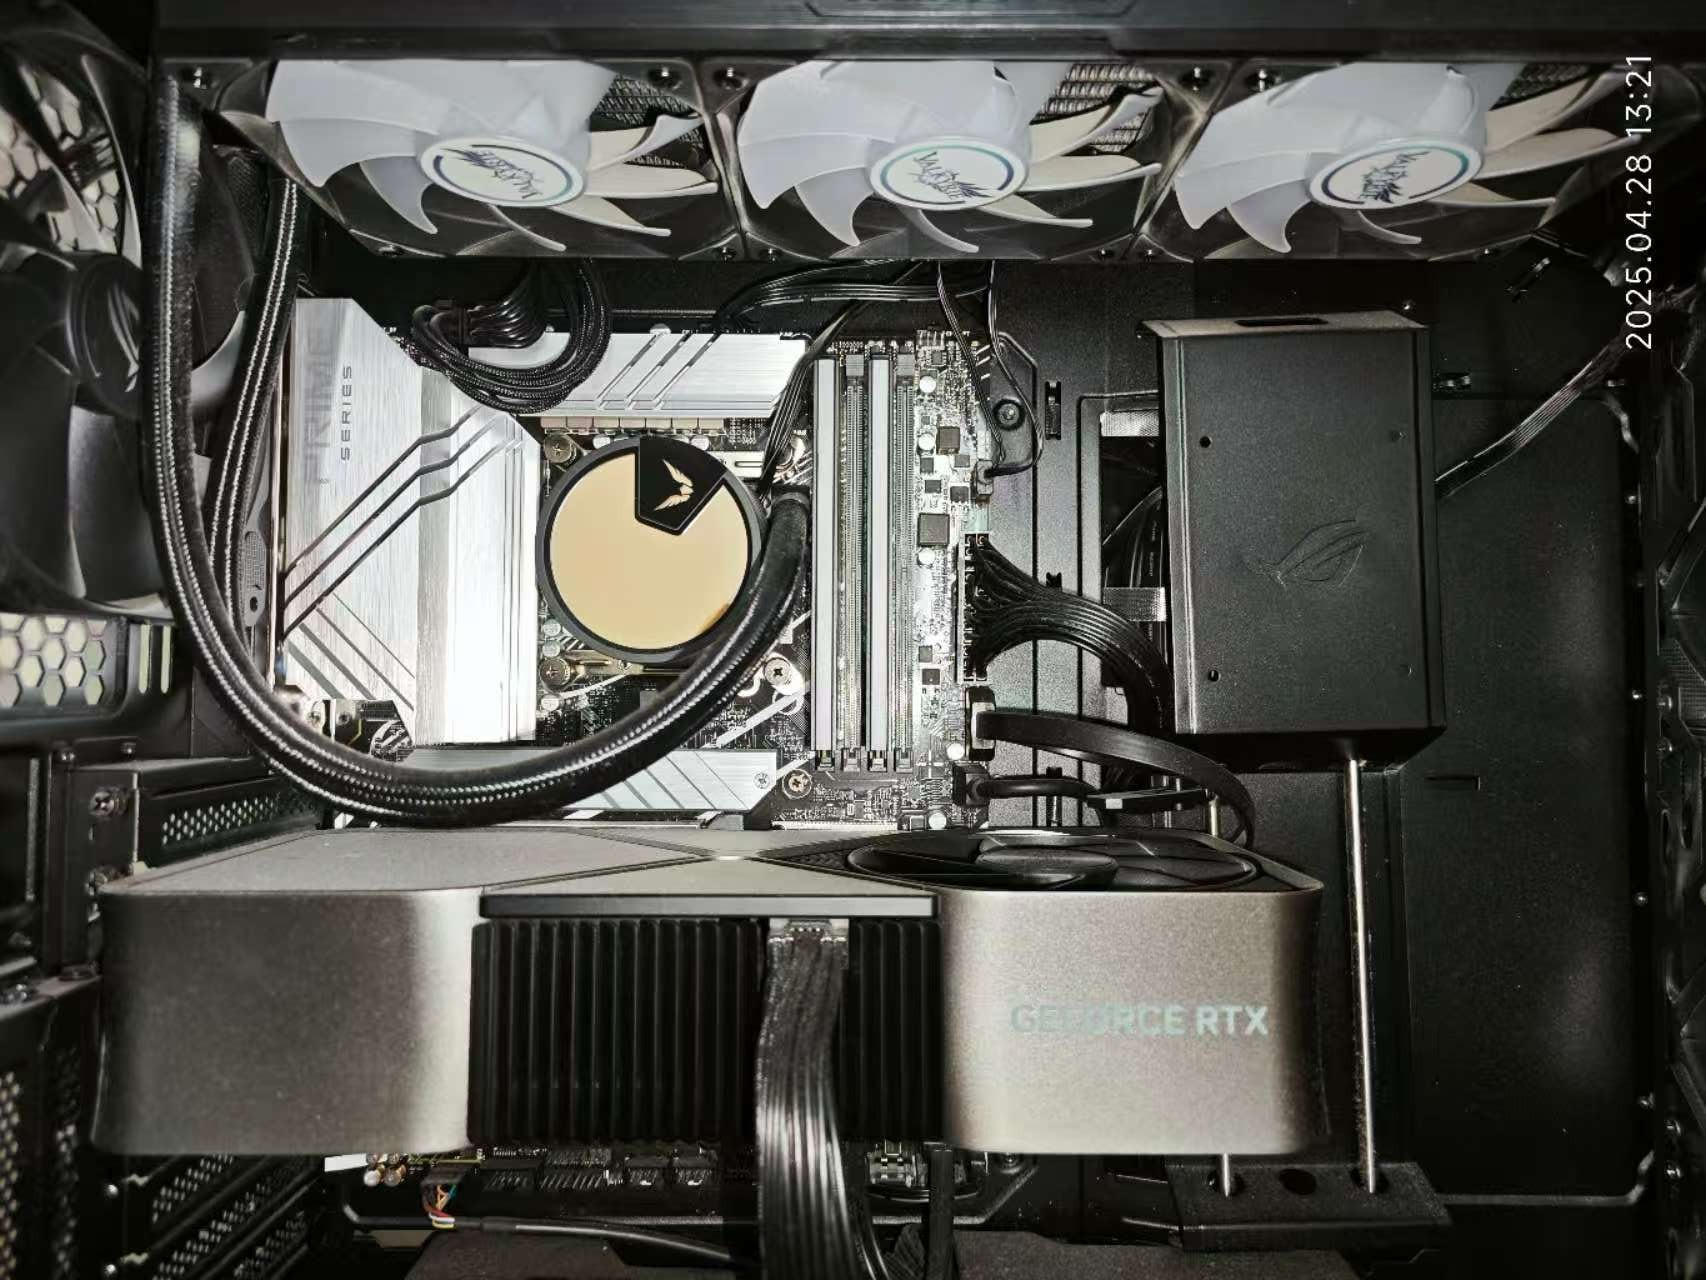
\includegraphics[width=0.8\textwidth]{100/hardware1.jpg}
  \caption{计算机的主机设备}
  \label{fig:computer-hardware}
\end{figure}

\subsubsection{中央处理器(CPU)}

CPU是计算机的最核心部件,它从存储设备读取指令和数据,并且执行这些指令。尽管现代处理器对代码和数据会有不同的处理,但是从程序员视角来看,其本质上都以二进制存储。代码由一条一条的指令组成,CPU 按照顺序一条一条执行从存储设备中读取的指令(至少从软件和程序员等使用者的视角看是这样),指令可以是修改 CPU 的状态,进行运算,或者是从其他硬件读取信息或者输出信息。如果希望进一步学习CPU如何运作等相关知识,可以参考著名的教材《CSAPP》,也可以修习《计算机系统导论》(ICS)这门课。

\subsubsection{内存(RAM)}

内存是计算机的临时存储器,它用于存储正在运行的程序和数据。它能够被CPU直接访问,因此速度较快。对于程序员而言,内存可以被抽象为一堆连续的存储单元,每个存储单元都有一个唯一的地址;执行程序时,程序的一部分或者全部被放进内存中,CPU就在内存中找寻需要的数据或者指令,如同在排列整齐的书架上寻找需要的书籍。

现代计算机内存读写速度很快,但是已经跟不上CPU的速度,因此又引入了高速缓存来加速内存的读写速度。高速缓存是内存和CPU之间的一个小型存储器,它存储了最近使用的数据和指令,以便CPU可以更快地访问它们。在断电以后,内存中存储的数据会丢失,因此内存也被称为是易失性的存储器。

\begin{note}
  上述文本中的“内存”指的是“随机存取存储器”(RAM)。这里的“随机”指的是可以在任意时刻访问任意地址,而不是“顺序存取”的存储器(例如磁带)。同时,“内存”这个词在部分语境下存在不同的含义,例如在BIOS语境下的“内存”指的是“只读存储器”(ROM),在移动设备(手机)等语境下的“内存”指的是“闪存”,这实际上是外存。
\end{note}

\subsubsection{外存}

外存是现代计算机的主要存储设备,用于存储操作系统、应用程序和数据等内容。其读写速度往往比内存慢得多,但是它的存储容量更大且往往是非易失的(相对内存而言)。

现代计算机的主要外存设备是硬盘。硬盘可以分为机械硬盘(HDD)和固态硬盘(SSD)。机械硬盘使用磁头在旋转的磁盘上读取和写入数据,而固态硬盘使用闪存芯片来存储数据。固态硬盘的读写速度比机械硬盘快得多,现在价格也便宜得多,但是使用寿命较短,且因为电荷流失等问题无法接受长期不通电等情况,不适宜作为长期存档介质(个人使用寿命和HDD无明显差异,基本都能用到彻底换机),除非花高价买高端的企业级SSD,但仍需定期通电。

除硬盘外,还有其他外部存储设备。例如:
\begin{itemize}
  \item U盘:一种小型的闪存存储设备,通常通过USB接口连接到计算机上。虽然和SSD都使用闪存颗粒,但是SSD通过主控优化、多通道技术等实现更高的性能,U盘则只用于低成本的便携存储。
  \item 光盘:一种使用激光读取和写入数据的存储介质。常见的光盘有CD、DVD和蓝光光盘,现在常用于单次写入的存档等。缺点是容易划伤和损坏,且信息密度低,读写速度慢。
  \item 磁带:一种使用磁性材料存储数据的介质,通常用于备份和存档。磁带的读写速度极为缓慢(和倒带速度成正比)且需要专门的设备来读写,设备价格昂贵,维护成本高。其优点是可靠性高,存储密度高。
  \item 软盘:一种老古董,使用磁性材料存储数据。现在软盘因为存储容量小、速度慢、易损坏等缺点,已经被淘汰了。
\end{itemize}

\begin{note}
  现代Windows系统的计算机中盘符默认从C开始而不是从A开始,正是因为AB盘符是给软驱用的;但是硬盘盘符从C开始的传统保留了下来,成为Windows的一个标志性特征。虽然现代的Windows系统允许手动分配盘符(如将C盘强行分配盘符A),但这样会导致系统不稳定,极不建议这么做。
\end{note}

\begin{caution}
\textbf{硬盘有价,数据无价。}请务必定期备份数据,尤其是重要数据。
\end{caution}

\subsubsection{显卡}

显卡是计算机的图形处理器,它用于处理图形和视频数据。显卡可以加速图形渲染,提高游戏和视频播放的性能。显卡通常有自己的内存,用于存储图形数据,被称为“显存”。

对于现在AI时代而言,显卡因为有着良好的并行特性,成为了深度学习的首选硬件之一。显卡的计算能力通常用“浮点运算每秒”(FLOPS)来衡量,通常情况下,显卡在机器学习等需要大量并行的简单计算工作上,表现远好于CPU。

\subsubsection{主板}

主板是一块电路板,将所有的硬件设备连接起来。主板上的芯片组负责协调各个硬件之间的通信。同时,主板还有一系列外部接口,用于连接外部设备。

\subsubsection{电源}

电源是计算机的电源供应器,它不参与数据存储与运算等操作,但能够为计算机的各个部件提供所需的稳定工作电压和电流。优质的电源能够避免计算机在运行过程中出现故障,延长计算机的寿命。

\subsubsection{输入输出设备}

输入输出设备指的是计算机与外界进行信息交互的设备。输入设备用于将用户的输入转换为计算机可以理解的格式,而输出设备则将计算机处理后的数据转换为用户可以理解的格式。

最古老的输入设备是拔插电缆,后来变成打孔纸带;现代常见的输入设备包括键盘、鼠标、扫描仪、麦克风等;现代常见的输出设备例如显示器、打印机、音响等。

\subsection{计算机的软件}

计算机的软件指的是计算机的程序和数据的集合。它可以分为系统软件和应用软件两大类。

\subsubsection{操作系统}

操作系统是计算机的核心软件,它负责管理计算机的硬件和软件资源。操作系统提供了一个用户界面,使用户可以与计算机进行交互。我们可以认为操作系统是连接现代软件和硬件的桥梁。目前,常见的操作系统有Windows、macOS、Linux等。

\textbf{Windows}\faWindows 是目前占有市场份额最大的操作系统。它由微软公司开发,广泛应用于个人计算机。Windows以其易用性和兼容性而闻名,广泛支持各种软件和硬件设备,但是缺点是在多数开发场景中的配置非常复杂,但是通过WSL2等工具也可以弥补一部分,且对于游戏开发等场景Windows仍是首选(主要是因为新游戏几乎都需要先适配Windows)。另一方面,Windows的安全性相对较低,容易受到病毒和恶意软件的攻击。

\textbf{macOS}\faApple 是苹果公司开发的操作系统,专门用于苹果的计算机产品。macOS以其优雅的界面和强大的功能而闻名,同时安全性相当高。缺点也很明显,macOS的硬件和软件生态系统相对封闭,且只能在苹果的硬件上运行,因此价格较高。

\textbf{Linux}\faLinux 是一个开源的操作系统,它是一个类UNIX操作系统。其学习曲线陡峭,至今在传统个人计算机市场的占有率仍然远低于Windows和macOS,但在服务器和嵌入式系统使用一直占据主导地位。Linux的开源特性使得它可以被自由修改和分发,因此有很多不同的Linux发行版,例如Ubuntu、Debian、Arch等。

几个系统的比较见下表:

\begin{table}[ht]
  \centering
  \begin{tabular}{c|ccc}
    \toprule
    操作系统 & Windows & macOS & Linux \\
    \midrule
    使用难度 & 简单 & 简单 & 较复杂 \\
    价格 & 收费 & 收费 & 免费 \\
    硬件兼容性 & 高 & 低 & 中高到极高 \\
    软件生态 & 丰富 & 不太丰富 & 丰富 \\
    安全性 & 较低 & 高 & 高 \\
    可定制性 & 低 & 低 & 高 \\
    社区支持 & 强 & 一般 & 强 \\
    适用场景 & 办公、游戏 & 设计、开发 & 服务器、开发 \\
    \bottomrule
  \end{tabular}
\end{table}

对于计算机新手,我们推荐使用Windows和macOS系统作为操作系统,这是因为它们提供了友好的用户界面和丰富的软件支持,适合初学者使用。对于希望深入学习计算机的初学同学,我们推荐使用Linux系统的发行版Ubuntu,因为它具有和Windows与macOS类似的图形界面,并具有良好的社区支持和丰富的学习资源。对于希望进阶的同学,我们推荐使用Arch Linux,它是一个轻量级的Linux发行版,具有高度的可定制性和灵活性。

\begin{figure}[ht]
  \centering
  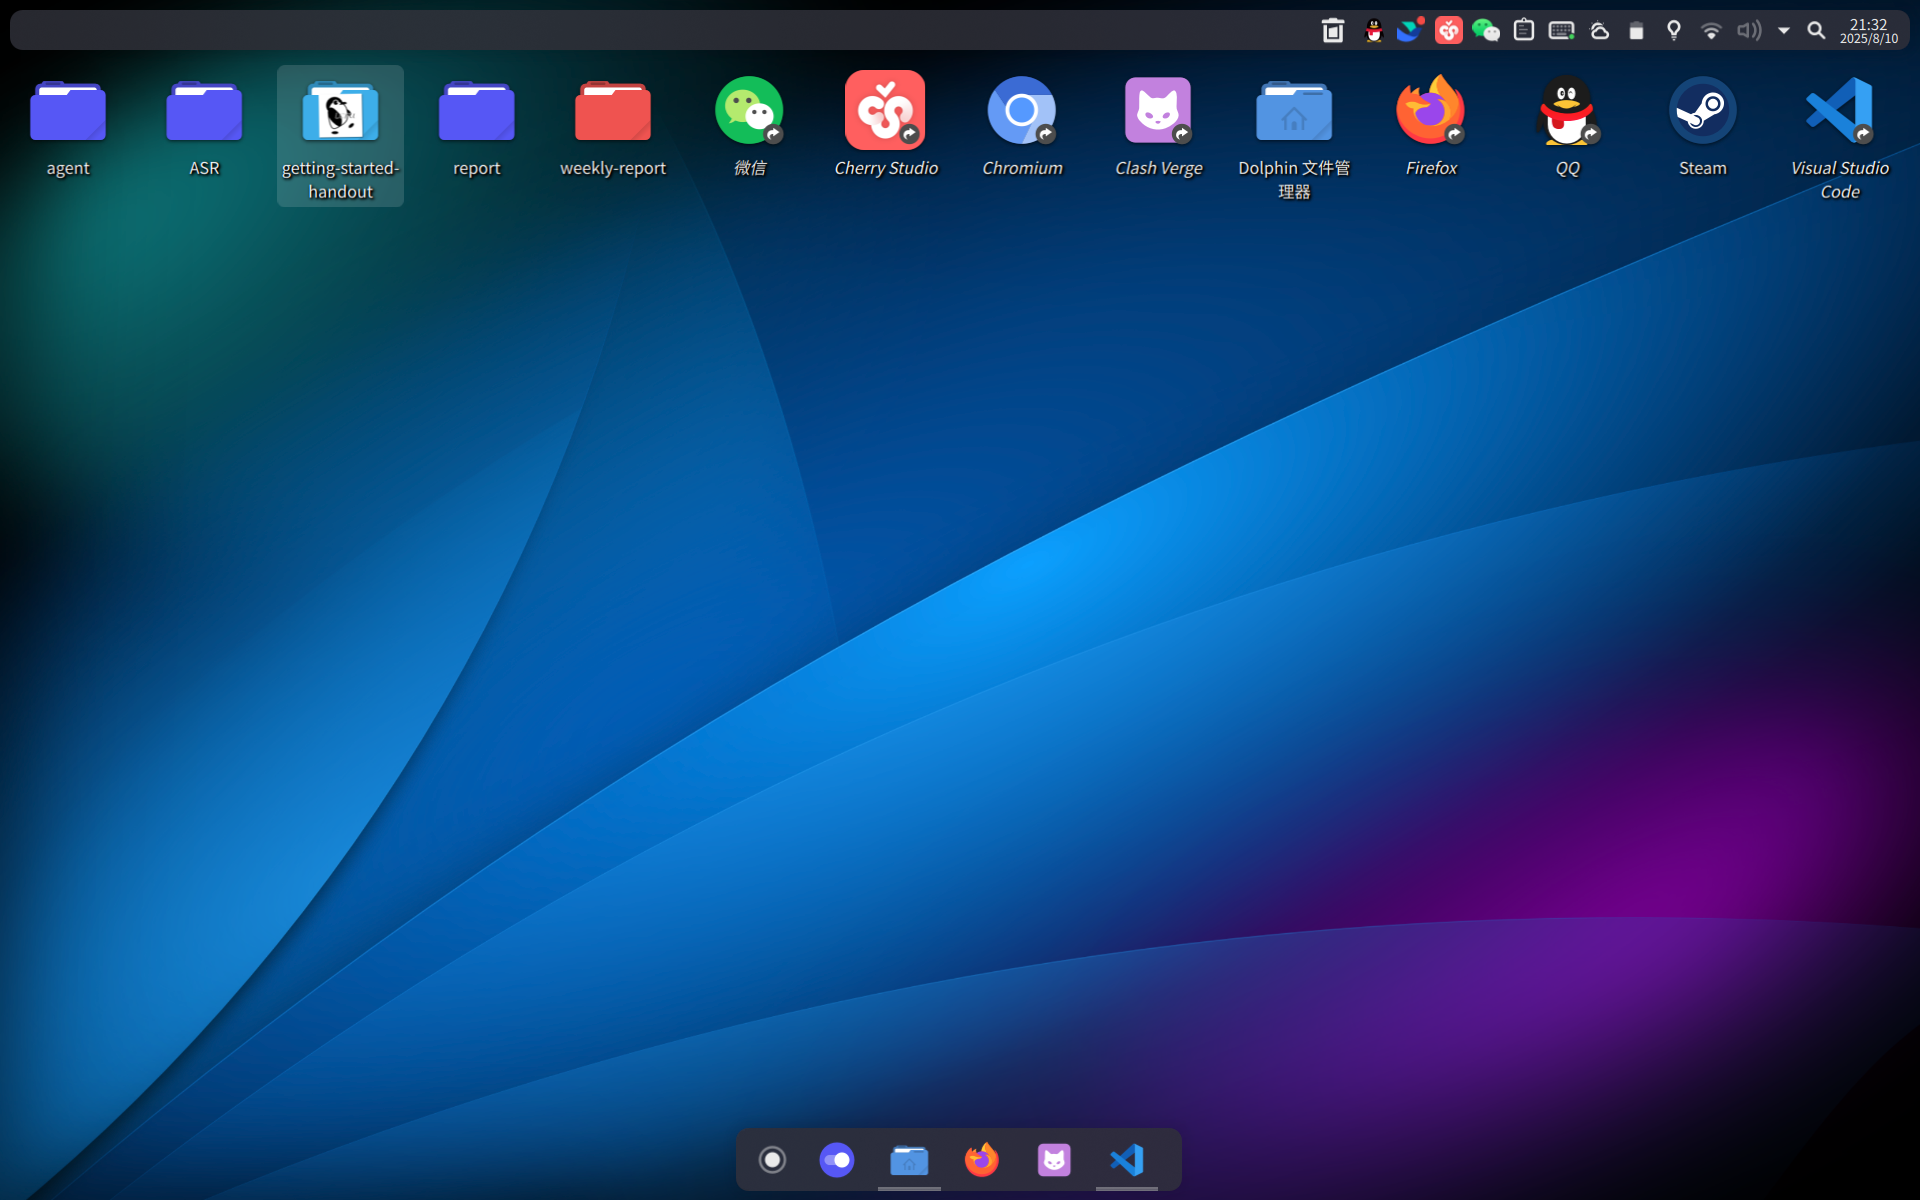
\includegraphics[width=0.8\textwidth]{100/fake-mac.png}
  \caption{一台假装自己是macOS的Arch Linux机器}
\end{figure}

\subsubsection{驱动程序}

驱动程序是操作系统和硬件之间的桥梁,它负责将操作系统的指令转换为硬件可以理解的语言。驱动程序通常由硬件制造商提供,并且在操作系统安装时自动安装。驱动程序的作用是使操作系统能够正确地识别和使用硬件设备。

驱动程序通常是特定于硬件的,因此不同的硬件设备需要不同的驱动程序。操作系统通常会自动检测硬件设备并安装相应的驱动程序,但是有时候需要手动安装驱动程序。我们可以到软件官网上下载最新的驱动程序,或者使用操作系统自带的驱动程序更新工具来更新驱动程序。不推荐使用“驱动精灵”等第三方驱动程序更新工具,因为它们可能会安装不必要的驱动程序,甚至可能会导致系统不稳定。

\subsubsection{应用软件}

应用软件指的是我们具体用于实现某一功能的工具。这类软件有很多,我们常用的通讯软件QQ、微信等,浏览网页的Chrome、Edge等,都是应用软件。

\section{计算机间的通讯}

计算机的通讯是指计算机之间或者计算机与其他设备之间进行信息交换的过程。目前计算机间的通讯主要是靠网络来实现的。网络是由许多计算机和其他设备通过通信协议连接在一起的系统,两大要素是\textbf{网络协议}(数据要依赖统一的协议传输)和\textbf{网络设备}(用于连接的设备)。

\subsection{网络基本名词及其解释}

不论是修电脑,还是平常使用计算机联网工作,我们总会在一些场合听到一些网络名词,这些网络名词不乏有被误解的。下面我们将对一些常见的网络名词进行解释。

\subsubsection{带宽、传输速率、延迟和丢包率}

这四个名词用来衡量网络的性能,是日常生活中最常见的几个名词。

首先,我们应当知道,文件这些东西都是“数据”,有一定的大小。现代计算机使用二进制来表示数据,规定一个二进制位为1比特(bit),8个二进制位为1字节(Byte)。在计算机上为了方便读取,之后的数据大小单位以$2^10=1024$为倍数递增,即1KiB=1024B,1MiB=1024KiB,1GiB=1024MiB,1TiB=1024GiB。\footnote{Windows系统中的KB指的实际上是KiB,这个是Windows本身的问题!而Linux和macOS则会正常显示KiB等。}另外一套单位系统以1000为倍数递增,也就是1KB=1000B,1MB=1000KB,1GB=1000MB,1TB=1000GB。这种标定方式通常由硬件厂商使用,因为便于硬件的生产,我们在日常生活中看到的硬盘、U盘等存储设备的容量使用的就是这种方式。因此购买的硬盘,计算机认为的容量会比标定容量小一些——这是正常现象,没有人偷你的空间。在TB之上还有更大的PB、EB等单位,但我们日常生活中用不到。

\begin{caution}
  有些无良卖家会使用这种单位:32Gb U盘,然后买到手发现只有4GB。这是因为该厂商使用了Gb(Gbit)而不是GB(GByte)来混淆视听,也就是32Gb=4GB,他甚至还没说谎,买家也只能打落牙齿往肚子里吞了。因此,购买存储设备时请务必注意单位究竟是什么。
\end{caution}

\textbf{带宽}指的是网络的理论最大传输能力,通常以比特每秒(bps)或字节每秒(B/s)来衡量。带宽越大,网络的传输能力就越强。例如,一个带宽为100Mbps的网络理论上可以每秒传输100兆比特的数据。我们家里通网的时候说的“千兆宽带”指的就是该网络的贷款是1000Mbps=1Gbps,或125MB/s。

而传输速率、延迟、丢包率则用于衡量网络的实际表现。\textbf{传输速率}指的是网络的实际传输速率,单位也是比特每秒(bps)或字节每秒(B/s),往往显著低于带宽。例如,一个带宽为100Mbps的网络可能实际传输速率只有50Mbps或更低。\textbf{延迟}指的是数据从发送方到接收方所需的时间,通常以毫秒(ms)为单位来衡量。延迟越低,网络的响应速度就越快。例如,一个延迟为50ms的网络意味着数据从发送方到接收方需要50毫秒的时间。\textbf{丢包率}指的是在数据传输过程中丢失的数据包的比例,通常以百分比(\%)来衡量。丢包率越低,网络的可靠性就越高。例如,一个丢包率为1\%的网络意味着在每100个数据包中有1个数据包会丢失。延迟、丢包率、传输速率等指标往往会受到网络拥塞、信号干扰、硬件性能等因素的影响。

\begin{example}
  有一辆满载硬盘的卡车从北京开到上海,估计其平均传输速率、延迟和丢包率,并和现在家用网络进行对比。
\end{example}

\begin{answer}
  先估算带宽。国内高速允许最大总重量为49吨(半挂或板车),一辆半挂车空车质量在16吨以上,这里为了方便按19吨计算,因此装载了30吨的硬盘。一块企业级数据盘容量按30TB($3\times 10^{13}$ B)计算,自重约700克;算上保护盒等,按1kg计算,因此一辆卡车装了$3\times 10^4$块硬盘,总容量为$9\times 10^{17}$ B,或者0.9EB。

  卡车在高速公路上最大时速在100到90千米每小时不等。按90千米每小时计算,北京到上海约1200千米,则行驶时间大概13.3小时,即$4.8\times 10^4$秒,因此传输速率用总数据量除以时间,得到约$1.9\times 10^{13}$B/s,即19TB/s,约合\textbf{152Tbps}。该数字非常惊人,是目前家用网络的近两万倍。

  下面估计延迟。和常规网络按数据包发送的方式不同,卡车运输是整体运输,或者说卡车本身就是一个大“数据包”,因此延迟等于运输时间,也就是从北京到上海的时间,约13.3小时,即\textbf{$4.8\times 10^4$秒}。

  下面估计丢包率。只要这个车没出事故、没被劫持、没整个掉沟里,那么就可以用公路运输HDD货物损失率0.02\%到0.05\%来充当丢包率。另外,如果出事故,则丢包率为100\%,而按照中国相关统计数据,公路运输百万公里事故数约为1起,因此完全可以忽略不计。综上,\textbf{丢包率约为0.05\%}。

  相对的,现在家用网络的传输速率大概在100MB/s到1GB/s之间,延迟大概在10ms到100ms之间,丢包率大概在0.1\%到1\%之间。可以看到,卡车运输的传输速率远远高于家用网络、丢包率显著低于家用网络,能和最优质的光纤媲美,但是延迟则高得离谱,完全无法进行实时操作。另外,卡车运输还受天气、交通等因素影响,稳定性无法和网络传输相提并论。
\end{answer}

在以往的计算机教材中总是出现一句话:“永远不要小看一辆满载磁带的卡车,其带宽远远超过了家庭网络。”看起来现在也差不多,只不过是把磁带换成了硬盘罢了;实际上,即使是2025年,把1EB数据从北京运到上海这个任务,最经济、最快速的方案依然是物流,其速度甚至能把5GB/s的高端光纤专线按在地上摩擦,成本更是低得多;只要不是那么要求时效性,物流依然是传输超大量数据的首选方案。

上述例子也提示我们怎么选择数据传输方式:GB级别的数据,可以使用任意网络途径传输;TB级别的数据,考虑使用专业的数据传输服务;PB级别的数据,考虑走光纤专线;EB级别的数据,则应考虑物流途径。要是数据量更大,那比起你把数据运过去,不如让对面把计算任务运过来。当然,上述数据是对于企业级别的网络而言的,个人用户的网络情况往往更极端,TB级别数据就可以考虑走快递等物流途径了;例如想把某些大文件从大连运送到沈阳,走网络可能需要几天时间才能传输完,而自行开车一天就能送到。

\subsubsection{IP地址和端口号}
IP地址是计算机在网络中的唯一标识符,类似于“门牌号”。目前有两种通行的IP地址:IPv4和IPv6。IPv4地址是一个32位的二进制数,通常用点分十进制数表示(例如192.168.1.1)。IPv6地址是一个128位的二进制数,通常用冒分十六进制数表示。IPv6地址的引入是为了应对IPv4地址耗尽的问题。

端口号是计算机在网络中用于区分不同应用程序的标识符,类似于“房间号”。端口号是一个16位的整数,范围从0到65535。常见的端口号有80(HTTP)、443(HTTPS)、22(SSH)等。我们假设要指向某一个计算机上的某一个应用程序,那么我们需要指定该计算机的IP地址和端口号。IP地址和端口号一起构成了一个完整的网络地址,通常表示为“IP地址:端口号”(例如0.0.0.0:8000)。

\subsubsection{域名}
域名是计算机在网络中的人类可读的标识符,类似于“网站名称”。域名由多个部分组成,通常用点分隔(例如www.pku.edu.cn)。域名系统(DNS)将域名转换为IP地址,以便计算机可以通过IP地址进行通信。

\subsubsection{子网掩码、网关}

子网掩码是一个32位的二进制数,用于划分IP地址的网络部分和主机部分。它通常用点分十进制数表示,它与IP地址进行按位与运算后,可以得到网络地址。子网掩码的作用是将一个大的网络划分为多个小的子网,以提高网络的效率和安全性。

网关是计算机在网络中的出口,用于连接不同的网络。网关通常是一个路由器或者交换机等设备。

\subsubsection{内网和外网}

我们在日常生活中,常常会听到“内网”和“外网”这两个词。内网是指一个局域网内部的网络,通常用于家庭、学校或者公司等小范围的网络。内网中的计算机可以通过路由器或者交换机等设备连接到外网。外网是指互联网上的网络,通常用于连接不同的局域网和广域网。

内网和外网的IP地址往往是不同的。内网IP地址通常是私有的IP地址,仅在内网中有效(例如每一个地级市都可能有一个“二中”,但是在不同的市称呼“二中”指的不是同一个学校);而外网IP地址全球唯一,互联网可以访问(例如“东港二中”)。例如大名鼎鼎的\texttt{8.8.8.8}是Google的公共DNS服务器的IP地址,它是一个外网IP地址。如果在内网中访问该地址,则可能访问到的不是Google的DNS服务器,而是内网中的某个设备。

\subsubsection{MAC地址}

MAC地址是计算机网络接口的唯一标识符,类似于“身份证号码”。它是一个48位的二进制数,通常用冒分十六进制数表示(例如00:1A:2B:3C:4D:5E)。MAC地址用于在局域网中唯一标识一个设备。每个网络接口卡(NIC)都有一个唯一的MAC地址。MAC地址通常由设备制造商分配,并且在设备的硬件中存储。

\subsubsection{网络协议}

网络协议是计算机之间进行通信的规则和约定。它定义了计算机如何发送和接收数据,以及如何处理错误和异常等情况。常见的网络协议有TCP/IP、HTTP、FTP等。不同的网络协议适用于不同的应用场景,例如TCP/IP协议适用于可靠的数据传输,而HTTP/HTTPS协议适用于Web应用程序的通信、UDP适用于精度要求不太高的实时通信等。

\subsubsection{网络设备}

网络设备是用于连接计算机和其他设备的硬件设备。常见的网络设备有路由器、交换机、集线器等。\textbf{路由器}用于连接不同的网络,并且可以根据网络协议进行数据转发;\textbf{交换机}用于在同一局域网内连接多个设备,并且可以根据MAC地址进行数据转发;\textbf{集线器}用于将多个设备连接到同一个网络,但不具备智能转发功能。

\textbf{光网络单元}(光猫,ONU)是用于将数字信号转换为光信号的设备,通常用于连接到光纤。光猫可以将计算机发送的数据转换为模拟信号,并且将接收到的模拟信号转换为数字信号。家用的光纤宽带通常是通过光猫连接到互联网的。

目前家用的路由器往往集成了光猫和交换机的部分功能,因此我们往往不需要像以前一样购买一大堆设备了。

\subsection{校内网络配置指南}

\subsubsection{计算机如何联网}

数据通过网络的传输需要以“数据包”的形式进行。数据包是网络传输的基本单位,它包含了发送方和接收方的IP地址、端口号、数据等信息。数据包通过网络设备(如路由器、交换机等)进行转发,最终到达接收方。

一台具体的机器,进行联网的步骤如下:
\begin{enumerate}
  \item \textbf{物理连接}:使用有线或者无线的方式,将计算机连接到网络设备(如路由器、交换机等)。
  \item \textbf{IP地址分配}:计算机通过DHCP协议自动获取IP地址、子网掩码、网关和DNS等信息。
  \item \textbf{网络协议配置}:计算机根据网络协议栈(如TCP/IP)配置网络协议,确保数据包的正确传输。
  \item \textbf{应用层协议}:计算机通过应用层协议(如HTTP、FTP等)与其他设备进行通信。
  \item \textbf{数据传输}:计算机通过网络设备和协议,将数据包发送到目标设备,并接收返回的数据包。
\end{enumerate}

\subsubsection{有线连接PKU校园网}

我们可以通过有线连接PKU校园网的方式来联网。在宿舍或者有网线接口的地方,我们可以将网线插入计算机的接口,这样就可以直接连接到校园网和互联网。

校园网的网络安全比较一般,建议购买一个路由器,连接到网线接口上,然后通过路由器连接到计算机。这样可以提高网络的安全性和稳定性。

\subsubsection{无线连接PKU校园网}

你可以在支持无线网络的设备WLAN列表中找到以下和北京大学有关的无线网络:
\begin{itemize}
  \item PKU :不安全,不建议使用。
  \item PKU Secure:采用IEEE 802.1x技术,能为用户提供较为安全的加密链路连接,一般情况下建议使用这个网络。
  \item PKU Visitor:访客网络,学生不需要使用这个。
  \item My BJMU:北大医学部的无线网络。
  \item eduroam:全球教育科研网络,该网络可以在全球许多高校使用。
\end{itemize}
具体怎样连接PKU Secure网络,请参考\href{https://its.pku.edu.cn/setting_6.jsp}{PKU Secure连接指南};使用eduroam的同学也可以参考\href{https://its.pku.edu.cn/service_1_eduroam.jsp}{eduroam连接指南}。

\subsubsection{校外连接北大内网}

为方便北京大学校园网用户在校外(家中、出差或国外)访问校园网资源,计算中心提供了VPN服务,可安全地接入校园网,如同在校内一样方便地访问学校全部的内网资源与服务(如校内门户、电子期刊数据资源等)。

具体怎样操作是一件比较复杂的事情,建议参考\href{https://its.pku.edu.cn/service_1_vpn.jsp}{北京大学VPN}的指南进行操作。

\subsubsection{北大网盘}

北大网盘是北京大学为师生提供的云存储服务,用户可以通过北大网盘存储、共享和管理文件。北大网盘提供了大容量的存储空间,并支持多种文件格式的上传和下载。

具体的使用可以参照\href{https://its.pku.edu.cn/service_1_webdisk.jsp}{北大网盘指南}进行操作。

\subsubsection{PKU腾讯会议教育版}

为了解决腾讯会议教育版资源紧张、预约繁琐的问题,计算中心上线了“腾讯会议预约申请”系统。

具体使用可以参照\href{https://its.pku.edu.cn/service_1_webex.jsp}{腾讯会议教育版指南}进行操作。

\begin{warning}
  腾讯会议教育版只用于学习和工作用途,临时、小规模或其他用途的会议请使用个人账号。
\end{warning}

\subsubsection{北大邮箱及其在第三方客户端的配置(以OutLook为例)}

北京大学为每一个新生都提供了一个北大邮箱。新生的邮箱服务一般由网易提供,地址是\texttt{<学号>@stu.pku.edu.cn}。学校的部分重要通知会发送到该邮箱上,请同学们注意查收。

方便起见,我们往往习惯于将邮箱配置到第三方客户端(如Outlook、Thunderbird等)上,以便于管理和使用。我将以Outlook为例,介绍如何配置北大邮箱。

首先,打开Outlook,点击“文件”菜单,然后选择“添加账户”。在弹出的窗口中,选择“手动进行配置”。下文使用IMAP-SMTP协议进行配置。

\begin{table}[ht]
  \centering
  \begin{tabular}{c|c|c}
    \hline
    & \texttt{pku.edu.cn} & \texttt{stu.pku.edu.cn} \\
    \hline
    IMAP服务器 & \texttt{imap.pku.edu.cn} & \texttt{imaphz.qiye.163.com} \\
    IMAP端口 & 993 & 993 \\
    \hline
    SMTP服务器 & \texttt{smtp.pku.edu.cn} & \texttt{smtphz.qiye.163.com} \\
    SMTP端口 & 465 & 994 \\
    \hline
  \end{tabular}
\end{table}

在进行正确的配置之后,Outlook会自动连接到北大邮箱服务器,此时会提示你输入用户名和密码。用户名一般是你的邮箱地址,密码则是来自特定客户端的授权码。对pku.edu.cn用户而言,授权码需在北大邮箱中获取,详见\href{https://its.pku.edu.cn/announce/tz20250702100126.jsp}{通知原文};对stu.pku.edu.cn用户而言,密码应在网易邮箱客户端中获取(登录网易邮箱网页客户端后,\texttt{设置>客户端设置>客户端授权密码})。输入正确的用户名和密码后,Outlook会自动连接到北大邮箱服务器,并开始同步邮件。

\section{网安相关知识} % Section Over

\subsection{网络的风险}

虽然互联网的出现给我们带来了便利,但也带来了很多风险。部分人心术不正,使用互联网进行诈骗、盗窃、敲诈勒索等违法犯罪活动;而他们使用的主要手段是不定向的网络攻击,例如钓鱼、木马和病毒等。

钓鱼指的是使用伪造的网页、邮件等方式,诱骗用户输入个人信息,例如用户名、密码、银行卡号等。其目的通常是获取用户的私人信息,以方便对其进行后续的诈骗、勒索等活动。

木马这个词来源于神话中的“特洛伊木马”,原指在一只巨大的木马中藏匿士兵,诱骗敌人打开城门进而发动攻击。现在的木马指一种恶意软件,它伪装成合法的软件或者捆绑在合法软件中,诱骗用户安装。一旦安装,木马就可以在用户不知情的情况下,窃取用户的个人信息、打开端口等。例如,一种最古老且经典的木马是FTP木马,它会在用户的计算机上打开一个FTP端口,允许攻击者远程访问用户的计算机。

蠕虫指的是一种自我复制的恶意软件,它可以在计算机之间传播。蠕虫通常利用计算机系统的漏洞进行传播,一旦感染了一个计算机,就会自动复制自己并传播到其他计算机。蠕虫通常会消耗计算机的资源,导致计算机变得缓慢或者崩溃。一个很经典的蠕虫是“小邮差”,它通过发送带毒邮件进行传播,会占满计算机的网络带宽;一旦感染了计算机,就会自动发送带毒邮件给其他计算机。

病毒指的是一种恶意软件,它可以在计算机之间传播。病毒通常依附在合法的软件中进行传播。病毒通常会破坏计算机的文件、数据等,导致计算机无法正常工作。一个很经典的病毒是“CIH”,它会在每年的4月26日感染计算机,并破坏计算机上的所有文件。它与蠕虫的区别是,病毒不能自己传播,只能依附于其他软件传播;而蠕虫可以自我复制。

被上述恶意软件感染后,计算机会变得不稳定、产生额外的资源开销,甚至导致计算机崩溃、数据破坏,造成经济或其他损失。君子爱财取之有道,我们应该遵纪守法,不要为了炫耀技术或者获取经济利益而制作这些恶意软件。

\subsection{从根源断绝问题}

为了防止计算机受到感染和破坏,最简单的方式是从根源上解决问题。我们在日常使用网络的时候,应该遵循以下原则:

\textbf{不浏览不安全网页}:在浏览网页的时候,若不能确定安全性,则尽量避免浏览不明链接、下载不明文件;如果确实需要下载软件,应该到官方网站上下载。

\textbf{识别伪造网站}:当一个网站需要你输入个人信息时,应该仔细检查该网站的安全性;钓鱼网站通常会伪装成合法网站,例如使用HTTPS协议、与合法网站相似的域名等。我们可以通过查看浏览器地址栏中的锁图标、检查网站的证书、观察域名是否正确等方式来判断网站的安全性。北京大学计算中心每年都会主动制作钓鱼网站,测试本校教职工和学生抗钓鱼的能力。虽然被计算中心骗了是一件不太光彩的事情,也总比被其他人骗了好,至少不会损失钱财。

\textbf{保持系统和软件的更新}:系统和软件的更新有一大部分是安全更新。定期更新软件可以阻止恶意软件利用漏洞进行攻击。

\textbf{保持杀毒软件的自动检测功能开启}:这类检测功能可以帮助我们初步检测计算机上的恶意软件。虽然有时候存在令人诟病的误报,但是它们仍然是我们保护计算机的一道重要防线。

\textbf{使用密钥代替密码}:密钥是一种更安全的身份验证方式,它可以防止密码被窃取。除了常用的公钥-私钥对,密钥还可以是USB设备、手机等。使用密钥可以防止密码被窃取和破解。目前一些技术网站已经支持使用密钥登录,例如GitHub、Google等。而我们在登录远程服务器的时候,也建议使用密钥而非密码登录。

\textbf{使用强密码并定期更换}:如果不得不使用密码登录,建议使用复杂的密码,并定期更换密码。复杂的密码应该包含字母、数字和特殊字符,并且长度至少为8位。我们也可以使用密码管理器(例如BitWarden)来生成和管理复杂的密码。

\textbf{定期备份数据}:定期备份数据可以防止数据丢失和损坏。数据备份有一个321原则:3份数据,2种介质,1个异地备份。也就是说,我们应该至少有3份数据备份,其中2份存储在不同的介质上(例如移动硬盘和云存储),1份存储在异地(例如云存储)。这样,即使我们的数据损坏了,也可以迅速恢复来减少损失。

\textbf{善用沙箱}:沙箱是一种虚拟化技术,可以将应用程序隔离在一个独立的环境中运行。这样可以一定程度上防止恶意软件对计算机造成损害。我们可以使用虚拟机、Docker等工具来创建沙箱环境,对于不能确定安全性的程序可以在此类环境中运行。

\subsection{亡羊补牢,为时未晚}

如果发现自己被钓鱼,应该紧急冻结相关账户并迅速更改密码,防止进一步的经济损失。在接下来的一个月到数个月中务必慎之又慎,你的信息可能已经被泄露,招致电信诈骗的概率显著增高。

如果发现自己的计算机感染了木马、病毒、蠕虫等,此事比被钓鱼更加严重。你应该依次执行以下内容:

\begin{itemize}
  \item \textbf{立即结束进程}:如果你能定位具体是哪一个软件正在搞破坏,可以使用任务管理器结束该进程。不过大多数情况下我们无法确定具体是哪一个进程出问题,此时忽略这一步即可。
  \item \textbf{立即断网}:这是一种负责任的行为,可以防止病毒进一步扩散。仅在软件层面上切断网络并不足够,如果你的计算机使用有线网络应该拔掉网线,以防止恶意进程重新连接网络。
  \item \textbf{立即查杀}:你可以运行杀毒软件的查杀功能,如是旧种类的病毒,杀毒软件应对起来不会太难。
  \item \textbf{立即上报}:如果杀毒软件查杀失败,应该立即上报相关部门。这可能意味着新型病毒的出现,上报有关部门有利于他们做出迅速反应,可以减少损失。
  \item \textbf{立即重装系统}:彻底重新格式化硬盘并重装系统可以彻底地清除残留的病毒文件。这是没有办法的办法,但却是最有效的。
\end{itemize}

\section{初步使用计算机}

你已经死了,这里是地狱!

因为你生前总是对着一堆没品笑话哈哈大笑,所以我们决定对你实施最严厉的酷刑:

——观看什么都不会的大学生操作电脑!

他在使用 Excel,但是他不会用任何一个快捷键!哦天哪他的 Ctrl 键甚至是全新的……他连自动填充和方向键都不用!从 1 到 100 都是手打的!

他输入中文的时候只用两根食指!每输入完一个词,他都用鼠标去点候选词!他一分钟打 20 个字!

他想要居中标题,在标题前面打了一连串的空格!

他直接在百度上搜 “爱奇艺下载” ,他点进了华军软件园!他点了那个最大的 “高速下载”!他直接运行了 p2p 下载器!他没有取消任何一个勾选的捆绑程序,直接点了下一步!他的桌面上多了 4 个,不,5 个,不,6 个图标!

他的表格做好了!他直接保存到 wps 云端了!他不知道如何把这份表格发给他的导师!他点了分享按钮,给导师发了一个金山文档链接!这份表格在云端查看的时候彻底乱码了!

他正在下载破解版游戏,他得到了一个压缩包!噢他没有解压缩,直接在压缩软件里点开了 \texttt{game.exe}!游戏报错了!

他终于正确地安装了一个游戏!他把 \texttt{game.exe} 直接剪切到了桌面!点开之后又报错了!

他希望把室友电脑里的游戏拷贝到自己电脑里!他把桌面上的快捷方式直接拖到了自己的 U 盘里!插回自己电脑运行的时候又报错了!

他打开文件的方式是鼠标左键疯狂连点!他至少点了 10 次!天哪现在桌面上的弹窗都堆不下了!

他把 “\texttt{Doc1.docx}” 直接重命名成了 “实验报告”!他连后缀名都删干净了!现在他再也找不到打开这份文档的方法了!

他在微信上收到了一个文件,他需要把这个文件用邮箱发出去。噢他完全不知道该怎么操作!他在收件人这一栏输入了上司的手机号!他完全不知道如何添加附件!他也完全不知道微信文件保存到哪里了!他对着微信消息按右键复制,然后把文件名粘贴到了正文栏!

他需要下载一个视频!他在视频网页点击了 “下载”,浏览器开始下载腾讯视频客户端了!他开始安装了!他在客户端里下载了一个 .qlv 格式的文件!他直接把这个文件发给别人了!

感受痛苦吧!你甚至没法教会他们!

觉得眼熟?实际上,上述操作在大学生中并不少见。为了避免你也落入这种境地,下面我们介绍一些基本的计算机使用知识。

关于MS Office等办公软件的使用,建议同学们自行学习相关的教程,笔者个人特别建议使用LaTeX来代替Word和PowerPoint,而Excel则使用Python脚本或更专业的统计软件来代替。

\subsection{文件、目录及其管理}

文件和目录是计算机中最重要的概念之一,它们用于存储和组织计算机中的数据。

\subsubsection{理解文件和目录}

如果把硬盘看作一个图书馆,那么文件就可以看作是图书馆中的一本书。目录则可以理解为图书馆的房间、书架等,以及图书馆本身,用于组织和分类图书馆中的书籍。假如我想找到一本书,首先要知道它在哪个图书馆,其次是在哪个房间、哪个书架的哪个位置。这样就能够使用统一的方式来找到一本特定的书。

在Windows系统中,每一个硬盘\footnote{实际上往往是硬盘分区。在旧的计算机中,也往往叫做驱动器或卷。初学者暂时不必纠结这些概念,只需要知道有这个东西就好了。}都是一个“根”目录,相当于图书馆本身。每一个根目录都有一个盘符,例如C盘、D盘等。每一个根目录下可以有多个子目录,这些目录往往表现为文件夹的形式;每一个子目录下又可以有多个子目录,最终形成树状结构。每一个目录下可以有多个文件(相当于图书馆中的书籍)。对于一个特定的文件,从根目录到所在地的路径是唯一的,例如\texttt{C:\textbackslash Users\textbackslash username\textbackslash Documents\textbackslash file.txt}。这个完整写出来的路径叫做\textbf{绝对路径},它唯一地标识了一个文件的位置。

有时候,我们在图书馆找书的时候,知道同类的书籍往往放在一起。例如我们已经知道了这个书架上有某书第一卷,我们也知道同一个书架上还有第二卷,这时候就不需要再从图书馆的根目录开始找了,而是可以直接从这个书架上找。这时候我们可以说,第二卷的路径\textbf{相对于第一卷的路径}在同一个目录下。这个相对于某个目录的路径叫做\textbf{相对路径},它并不是唯一的,因为它依赖于当前所在的目录。举个例子,假如某文件\texttt{file1}在某目录下,同目录下还有一个\texttt{file2},那么\texttt{file2}相对于\texttt{file1}的路径就是\texttt{file2}。如果该目录下还有一个子目录\texttt{dir},该子目录下有一个\texttt{file3},那么\texttt{file3}相对于\texttt{file1}的路径就是\texttt{dir\textbackslash file3}。

有些时候,相对路径可能会跨目录,这时候就需要向上一级等操作。这时候,就可以使用“\texttt{..}”来表示上一级目录,使用“\texttt{.}”来表示当前目录。例如,假如某文件\texttt{file1}在某目录下,该目录的上一级目录下有一个\texttt{file2},那么\texttt{file2}相对于\texttt{file1}的路径就是\texttt{..\textbackslash file2}。同样,如果该目录的上级目录下还有一个子目录\texttt{dir},该子目录下有一个\texttt{file3},那么\texttt{file3}相对于\texttt{file1}的路径就是\texttt{..\textbackslash dir\textbackslash file3}。

\subsubsection{文件的扩展名}

扩展名是文件名中最后一个点后面的部分,例如\texttt{file.txt}的扩展名是\texttt{txt}。扩展名可以帮助操作系统识别文件的类型,并选择合适的程序来打开它。在Windows上,文件的扩展名往往是必须的,否则操作系统不能识别文件的类型。

在Windows系统中,文件的扩展名通常是隐藏的。如果你想查看文件的扩展名,可以在文件资源管理器中点击“查看”菜单,然后选择“文件扩展名”选项。这样就可以看到所有文件的扩展名了。为了方便维护目录等,笔者建议同学们选择显示扩展名。

\begin{table}[ht]
  \centering
  \begin{tabular}{c|l}
    \toprule
    常见文件类型 & 常见扩展名 \\
    \midrule
    文本文件 & .txt, .md, .log \\
    文档文件 & .doc(x), .xls(x), .ppt(x), .pdf \\
    图片文件 & .jpg, .jpeg, .png, .gif, .bmp, .svg \\
    音频文件 & .mp3, .wav, .flac, .aac \\
    视频文件 & .mp4, .avi, .mkv, .mov \\
    压缩文件 & .zip, .rar, .7z, .tar, .gz \\
    可执行文件 & .exe, .bat, .sh \\
    代码文件 & .c, .cpp, .py, .java, .js, .html, .css \\
    \bottomrule
  \end{tabular}
  \caption{常见文件类型及其扩展名}
  \label{tab:file-extensions}
\end{table}

一般情况下,虽然文件的类型差不多,但是其扩展名不同也往往代表着其数据的存储是按照不同的方式进行的。例如,\texttt{bmp}文件是“位图”,存储的是每一个像素的颜色信息;而\texttt{jpg}文件则是经过压缩的,存储的是图像的整体信息。对于同一张图片,\texttt{bmp}文件往往会比\texttt{jpg}文件大得多。如果我们试图将一个\texttt{bmp}文件改名为\texttt{jpg},那么这个文件的扩展名变了,但是\textbf{其内部数据并没有变},因此这个文件仍然是一个\texttt{bmp}文件,只不过扩展名变了而已。此时,如果我们使用图片查看器打开这个文件,图片查看器会根据扩展名来判断文件类型,认为它是一个\texttt{jpg}文件,但是实际上它是一个\texttt{bmp}文件,因此图片查看器可能无法正确地打开它。因此,技术人说的“一类文件”往往不是按文件的性质分类的,而是按文件的扩展名(数据的存储方式)分类的。

有时候,我们可能会需要更改文件的类型。从上面的例子可以看出,直接更改扩展名并不能改变文件的类型,因此我们需要使用专门的软件或者网站来帮助我们转换文件的类型。例如,我们想要将一个\texttt{bmp}文件转换为\texttt{jpg}文件,我们需要使用图片编辑软件(如Photoshop、GIMP等)或者在线转换工具来进行转换。转换后,文件的扩展名和内部数据都会发生变化,变成一个真正的\texttt{jpg}文件。

\subsubsection{文件的打开方式}

对于任何文件,我们往往需要读取其中的数据,这个文件才有意义;至于这个数据是怎么展示的则另当别论。因此,我们需要一些软件来帮助我们打开文件。

在Windows系统中,文件往往有一个默认的打开方式,这个打开方式由文件的扩展名决定。例如,\texttt{.txt}文件默认使用记事本打开,\texttt{.jpg}文件默认使用照片查看器打开。有些时候安装了一些软件后,文件的默认打开方式可能会被更改。例如,安装了某个图片编辑软件后,\texttt{.jpg}文件的默认打开方式可能会被更改为该软件。

在一些情况下,我们可能会需要临时或永久更改某一类文件或者某一个文件的打开方式。我们可以右键点击文件,然后选择“打开方式”选项,选择一个合适的软件来打开该文件,也可以选择“选择其他应用”之后寻找指定的软件。如果我们想要永久更改某一类文件的默认打开方式,只需要在“选择其他应用”菜单勾选“始终使用此应用打开\texttt{.扩展名}文件”选项即可。

值得注意的是,软件本身并不需要扩展名才能打开文件。软件打开文件时总是按照自己的方式来处理数据,因此很多时候即使扩展名是错误的或者没有扩展名,如果指定了正确的软件,软件仍然可以正确地打开文件。

\subsubsection{文件的链接}

有时候,我们可能会需要在不同的目录中使用同一个文件或目录,这时候就可以使用文件的链接。文件的链接类似于图书馆中的索引卡片,它指向某个文件的位置,而不是文件本身。

在Windows中,文件的链接叫做快捷方式。我们可以右键点击文件,然后选择“创建快捷方式”选项,Windows会在当前目录下创建一个指向该文件的快捷方式。我们也可以将快捷方式移动到其他目录中使用。需要注意的是,快捷方式本身并不包含文件的数据,因此如果原文件被删除或者移动,快捷方式往往无法正常工作。另一方面,即使我们对快捷方式进行任意的删除或移动,原文件仍然完好无损。

上述建立链接的方式叫做软链接(符号链接)。与之相对的是硬链接,硬链接是指多个文件名指向同一个文件的数据。硬链接的创建和管理比较复杂,一般不建议初学者使用。

\subsubsection{文件的压缩与解压}

有时候文件占据了过大的空间,或者因为文件数量太多而不便于传输和管理,这时候我们可以使用文件压缩工具来将文件进行压缩。文件压缩工具可以将多个文件或者目录打包成一个文件,并且可以对文件进行压缩,以减少文件的大小。常见的文件压缩格式有\texttt{.zip}、\texttt{.rar}、\texttt{.7z}等。

笔者个人推荐使用\texttt{7z}压缩软件来压缩和解压文件。它是一个经典的开源软件,支持多种压缩格式,并且具有较高的压缩率。一般情况下,在我们安装了\texttt{7z}软件之后,右键点击文件或者目录,就可以看到“添加到压缩文件”选项,点击该选项即可将文件或者目录进行压缩。对于压缩文件,我们也可以右键点击,然后选择“解压到当前目录”选项,或者选择“解压到\texttt{文件名}\textbackslash”选项,将文件解压到指定的目录中。

不同的压缩参数会产生不同的效果。把固实数据大小开大则会提高压缩率\footnote{压缩率是指压缩后的文件大小与原文件大小的比值,压缩率越高,说明压缩效果越好。},但会牺牲压缩和解压的速度;勾选了分卷,则会将压缩文件分割成多个小文件,便于诸如\texttt{FAT32}等不支持大文件的文件系统存储;使用内存和CPU则显著影响了压缩的速度;不同的压缩算法则会影响压缩率和速度的平衡。一般情况下,默认参数已经足够好用了,软件本身也提供了多种预设参数供我们选择。

至于压缩成的文件格式,笔者比较推荐使用\texttt{zip}格式,其兼容性最好;如果对压缩率有较高要求,可以使用\texttt{7z}格式。不建议使用\texttt{rar}格式,因为它是一个专有格式,虽然压缩率不错,但是不够开放。

\begin{caution}
  有些软件的可执行文件和附带文件是通过压缩包分发的;有些文件也是通过压缩包传输的。在这种情况下,我们一定要先解压文件,再使用文件,而不是在压缩包中直接使用文件,这样可能会导致文件无法正常工作。
\end{caution}

\subsubsection{Windows的文件系统结构}

Windows使用的是NTFS文件系统,基于驱动器(Drive),每个驱动器都有一个盘符(例如C:、D:等)。每个驱动器既可以是一个物理存储设备,也可以是一个存储设备的某一分区(主分区或者逻辑分区)。Windows的文件系统结构是树形结构,每个驱动器下都有一个根目录(例如C:\textbackslash),根目录下可以有多个子目录和文件。

在Windows下,路径使用反斜杠(\textbackslash)作为分隔符。例如\texttt{D:\textbackslash dir\textbackslash file.txt}。尽管如此,Windows也支持使用正斜杠(/)作为分隔符,两者也可以混合使用。不过我们建议在Windows下使用反斜杠(\textbackslash)作为分隔符,以保持一致性。

Windows中有如下一些常用的文件夹:
\begin{itemize}
  \item \texttt{C:\textbackslash Windows}:Windows操作系统的核心文件夹,包含系统文件和驱动程序。
  \item \texttt{C:\textbackslash Program Files}:安装的应用程序的默认文件夹,通常包含64位应用程序。
  \item \texttt{C:\textbackslash Program Files (x86)}:安装的32位应用程序的默认文件夹。
  \item \texttt{C:\textbackslash Users}:用户文件夹,包含每个用户的个人文件和设置。
  \item \texttt{C:\textbackslash Downloads}:下载文件夹,默认存储从互联网下载的文件。
\end{itemize}

\subsubsection{高效的文件管理}

从一大堆文件中快速找到我们想要的文件是一个非常重要的技能。

一个常用的手段是使用搜索功能。Windows文件资源管理器提供了搜索功能,可以帮助我们找到文件。我们可以在文件资源管理器的右上角输入关键词,文件资源管理器会自动搜索当前目录及其子目录中的文件,并显示匹配的结果。然而,文件管理器的搜索面对大量文件时效率很低。这时候,我们可以使用一些第三方的搜索工具,例如Everything、Listary等。这些工具可以快速索引计算机中的文件,并提供快速的搜索功能。它们通常比文件资源管理器的搜索功能更快、更强大。

另一个常用的手段是养成良好的存储习惯,将相关的文件放在一起,使用有意义的文件名和标签、分类等工具。Windows没有内置的标签功能,但我们可以使用一些第三方的标签工具,例如TagSpaces、FileMeta等。对于大量的文件,我们可以使用自动化脚本来帮助我们管理文件,例如使用Python脚本来批量重命名文件、移动文件等。

\subsection{怎样安装软件}

我们下载软件的主要渠道有两种:通过官方渠道下载、通过包管理器(Winget,Homebrew,apt等)下载。这两种渠道一般认为是最安全且问题最少的。官方渠道包括软件的官方网站、操作系统提供的应用商店(Microsoft Store、App Store)等;包管理器是用于管理软件包的工具。它可以自动下载、安装、升级和卸载软件包,并且可以解决软件包之间的依赖关系。

在Linux和macOS中,包管理器是非常常用的工具。它可以帮助用户快速安装和管理软件包,避免手动下载和安装软件包的麻烦。比如我希望在Arch Linux下安装GCC,只需要执行以下命令即可:

\begin{lstlisting}[language=bash]
    sudo pacman -S gcc
\end{lstlisting}

在Windows中,包管理器的使用不普遍。虽然有一个官方的包管理器winget,但是支持的软件包较少,且无法自动管理依赖(但也基本够用);还有一些例如Chocolatey、Scoop等第三方包管理器。除此以外,使用MSYS2、Cygwin等类UNIX环境也可以从某种程度上当成包管理器使用。例如后文讲的安装GCC的过程,我们就是使用MSYS2来安装的,比下载预编译版本简单许多。

我们并不推荐在非官方渠道下载软件,这些非官方渠道往往以某某软件站、某某下载站、某某应用商店(Microsoft Store这类系统自带的除外)等形式出现。通过上述方式下载的软件可能导致使用盗版、附带流氓插件甚至木马、病毒等问题,或者遇到一些其他各种问题。

如果不使用包管理器安装软件,则从官方渠道等下载的软件往往是一个压缩包或者一个可执行文件(安装包)。对于压缩包,我们只需要解压到某个目录即可使用;对于安装包,我们需要运行安装包,然后按照提示进行安装即可。为了防止过量占用C盘空间,我们建议将软件安装到非系统盘(C盘)中,例如D盘、E盘等;有些软件在安装时可能会允许你将该软件加入到系统的PATH环境变量中,我非常建议大家这么做。

\subsection{怎样卸载软件}

我们不推荐反复装卸软件,因为这可能会导致系统不稳定或者软件残留。但是有些时候,我们认为某个软件长期内不会再需要了,且磁盘空间告急,这时我们应该考虑将其卸载。

计算机小白最喜欢做的一件事是把桌面上的快捷方式移动到回收站,这是非常错误的做法。快捷方式只是指向软件的一个链接,删除快捷方式并不会卸载软件本身。对计算机半懂不懂的人喜欢找到软件的安装目录,直接删除软件的文件夹,这也是错误的做法。因为对于许多软件而言,这样做会导致软件的注册表项和其他配置文件残留在系统中,可能会导致系统不稳定或者软件无法正常工作。

正确的做法有两种:要么使用计算机自带的“程序与功能”界面删除软件,要么使用软件自带的卸载程序(通常命名为uninstall.exe或者类似名称)。某些软件可能会在安装时提供一个卸载程序,我们可以在开始菜单或者软件的安装目录中找到它。使用这些方法可以确保软件被完全卸载,留下的残留文件也较少。如要彻底删除残留文件,可以使用一些专业的卸载工具,例如Geek等。

\subsection{北京大学正版软件}

为了保护知识产权、方便学生节约资金,北京大学购买了一系列常用软件的正版授权,方便师生使用。我们可以登录\href{https://software.pku.edu.cn/}{北京大学正版软件网站},使用自己的北大账号和密码登录,下载和安装这些软件。

\subsection{软件版权和开源协议}

虽然计算机是一个非常强大的工具,但是它也可能被滥用,造成严重的后果。因此,我们需要遵守计算机伦理、法律和合规要求,以确保我们使用计算机的行为是合法和道德的。有时候我们认为稀松平常的事情,也有可能被警告。比如说用爬虫爬取IEEE论文,可能就会被IEEE警告;或者在GitHub上上传了一些别人写的GPL代码,也有可能被GitHub报DMCA警告。因此我写了本节,以提醒同学们规避风险。

软件可以认为是“数字作品”,因此也受版权法的保护。一般软件有商业软件和开源软件两种。商业软件通常是收费的,用户需要购买许可证才能使用;而开源软件则是免费的,用户可以自由地使用、修改和分发。

商业软件一般遵循专有许可证,例如微软的Windows、Office等。这些软件的源代码是保密的,用户只能使用软件的二进制文件,也不能随意修改和分发软件。这类许可证一般被叫做Copyright。对于此类软件的盗版,即使是个人使用也面临侵权风险;如果是把它用于商业则风险更大,可能面临严厉的惩罚。

而与Copy'right'相对应的也有Copy'left',即开源许可证。开源许可证允许用户自由地使用、修改和分发软件,但是需要遵守一些规定。常见的开源许可证有GPL、MIT、Apache等。这些许可证一般要求用户在分发软件时附带原始许可证,并且在修改软件时注明修改内容。

以 GPL(GNU General Public License)为例,它是最具代表性的 Copyleft 许可证之一。GPL 的核心思想是:任何人都可以自由地使用、修改和再发布软件,但如果将修改后的版本公开发布(例如发布到网上或提供给他人使用),那么整个衍生作品也必须以 GPL 许可证发布。这意味着,基于 GPL 代码开发的软件也必须开源,从而确保“自由”能够延续下去。这种“传染性”特征使得 GPL 在开源社区中备受推崇,但也引发了一些商业公司的顾虑。

除了GPL以外,还有以下这些常见的开源许可证:
\begin{itemize}
  \item MIT:MIT许可证是一种非常宽松的开源许可证,允许用户几乎无限制地使用、修改和分发软件。唯一的要求是必须在软件中包含原始许可证和版权声明。MIT许可证非常适合那些希望最大限度地推广其软件的开发者。
  \item Apache:Apache许可证也是一种宽松的开源许可证,允许用户自由地使用、修改和分发软件。与MIT许可证类似,Apache许可证要求用户在分发软件时附带原始许可证和版权声明。此外,Apache许可证还包含了一些专利授权条款,允许用户在某些情况下使用专利技术。
  \item BSD:BSD许可证是一种宽松的开源许可证,允许用户自由地使用、修改和分发软件。与MIT许可证类似,BSD许可证要求用户在分发软件时附带原始许可证和版权声明。BSD许可证有多个版本,最常见的是3-Clause BSD和2-Clause BSD。
  \item MPL:MPL(Mozilla Public License)是一种中等宽松的开源许可证,允许用户自由地使用、修改和分发软件。与GPL不同,MPL允许用户将修改后的代码与闭源代码混合使用,但要求对修改过的文件进行开源。MPL适合那些希望在保护部分代码的同时,仍然参与开源社区的开发者。
\end{itemize}

值得一提的是,开源并不等于“没有限制”。虽然用户可以自由使用、修改和分发软件,但必须遵守相应的开源许可证条款。违反这些条款,比如未按要求附带许可证、未注明修改内容,或者将 GPL 代码用于闭源商业软件,都可能构成侵权行为,甚至引发法律诉讼。


\subsection{实用软件推荐}

在学习和工作中,我们常常需要一些实用的软件来提高效率。以下是笔者个人推荐的一些实用软件,以供同学们参考。这些软件中有些是免费的,有些是收费的,具体使用时请注意软件的授权和使用条款。同时,为了防止功能冗余,我们非常建议每类软件只安装\textbf{一个}(尤其是播放器和杀毒软件!)。

\begin{itemize}
  \item 下载器类
    \begin{itemize}
      \item Internet Download Manager(IDM):一个极为强大的收费下载软件,可以显著加速下载速度,并支持断点续传等功能。遗憾的是,它不支持磁力链接和BT下载。
      \item Free Download Manager(FDM),一个免费的下载软件,界面友好且现代,且支持磁力链接和 BT 下载。
      \item 比特彗星(BitComet):一个免费且经典的BT下载软件,支持磁力链接和BT下载。
      \item qBittorrent:免费且开源的 BT 下载软件。
    \end{itemize}
  \item 浏览器类
    \begin{itemize}
      \item Google Chrome:一个免费的浏览器,基于Chromium内核。
      \item Mozilla Firefox:一个免费的浏览器,基于Gecko内核。
      \item 油猴:一个浏览器扩展,可以让用户自定义网页的样式和功能。它可以通过安装脚本来实现各种功能,例如广告拦截、界面美化等。油猴支持多种浏览器,包括Chrome、Firefox等。这里推荐一个链接:\href{https://github.com/zhuozhiyongde/PKU-Art}{PKU-Art},它可以给你一个风格现代、足够好看的教学网。
    \end{itemize}
  \item 压缩与解压缩类
    \begin{itemize}
      \item 7-Zip:一个免费且强大的开源老牌压缩软件,支持多种压缩格式,包括7z、zip、rar等。它的压缩率高(7z格式压缩号称全球第一压缩率),速度快,功能强大。
      \item NanaZip:在 7-Zip 基础上提供更现代化的界面(Windows 11 风格),并增加对 ZStd、LZ4 等压缩算法的编解码支持。此外,它使用 MSIX 打包,因此可上架 Microsoft Store,且可以在 Windows 11 的默认右键菜单中直接使用,而无需打开扩展右键菜单。
    \end{itemize}
  \item 播放器类
    \begin{itemize}
      \item VLC Media Player:一个免费的开源播放器,支持众多音频和视频格式。
      \item MPV:免费且开源的播放器,支持格式众多。可以使用命令行、脚本或着色器来精细地控制播放器行为,但上手难度较高。
      \item PotPlayer:另一个免费的播放器。
    \end{itemize}
  \item 杀毒软件类(Mac和Linux因为其高安全性,通常不需要安装杀毒软件)
    \begin{itemize}
      \item Windows Defender:Windows系统自带的杀毒软件,功能强大,查杀率接近100\%,已经和老牌专业杀软(卡巴斯基、BitDefender等)不相上下,能够有效地保护常规情况下计算机免受病毒和恶意软件的侵害。但是误报率较高,可能会误报一些正常的软件为病毒。
      \item 火绒:一个免费的国产杀毒软件,误报率很低,界面友好,适合普通用户使用。然而,火绒的杀毒能力要低一些。
    \end{itemize}
  \item 其他
    \begin{itemize}
      \item Everything:一个免费的文件搜索工具,能够快速地搜索计算机上的文件。它的搜索速度极快,支持多种搜索方式,包括模糊搜索、正则表达式搜索等。
      \item Wallpaper Engine:一个收费的动态壁纸软件,能够让你的桌面变得更加美观。它支持多种动态壁纸,包括视频壁纸、动画壁纸等。
      \item Rufus:一个免费的U盘制作工具,能够将ISO镜像文件写入U盘,制作成可启动的U盘。它支持多种操作系统的ISO镜像,包括Windows、Linux等。
      \item Ventoy:一个开源的u盘启动工具,能够使多个ISO镜像共存于U盘,而不必格式化U盘,选择从其中的一个镜像启动。它能使多个镜像文件和U盘其他文件共存,是装机盘和资料盘合一的好工具。
      \item UltraISO:一个收费的光盘镜像制作工具,能够创建、编辑和转换光盘镜像文件。它支持多种光盘格式,包括ISO、BIN、CUE等。
      \item VMware/VirtualBox:两个免费的虚拟机软件,能够在计算机上创建虚拟机,运行其他操作系统,可以用于测试软件、学习操作系统等。
      \item Cherry Studio:一个LLM管理器,能够帮助你使用各种LLM来简单地创建Agent,来辅助你的开发和生活。
    \end{itemize}
\end{itemize}

\begin{tip}
对于macOS用户而言,卸载软件不需要上文叙述那么麻烦,只需要将应用程序拖到废纸篓中即可。或者也可以模仿Linux常见的卸载方式,使用包管理器(如Homebrew)来卸载软件。
\end{tip}

\subsection{字符和编码}\label{sec:locale}

我们知道,现在的计算机是使用二进制来存储数据的。但是,对于人类使用的语言而言,即使是相对简单的英语,也有52个大小写字母、10个数字、各种标点符号和特殊符号等,远远超过了二进制的0和1两种状态;而计算机却能够正确地显示并处理这些字符。这究竟是怎么做到的呢?

一个非常容易想到的办法就是,给每一个字符分配唯一的一个编号,然后再使用二进制来表示该编号。通过建立字符和编号之间的唯一映射关系,我们就可以使用二进制来表示字符了。如果把许多个字符和编号之间的映射关系放在一起,就叫做\textbf{字符集};至于如何建立字符和编号之间的映射关系,就叫做\textbf{编码方案}。

然而,一开始,不同厂家、不同地区等生产的计算机系统使用不同的编码方案,导致同一个编码在不同的系统上表现为不同的字符,对数据交换造成了严重的障碍。我们童年时候玩的新新魔塔就是一个非常典型的例子,其标题在中国的计算机上显示为“穝穝臸娥”,其中角色“暗黑大法师”被显示为“穞堵臸猭畍”,现在这个甚至成为了一个梗。

为了解决这个问题,也容易想到两种手段:要么利用一些方法来区分不同的编码方案,并在使用时指定编码方案;要么制定一个统一的编码方案,所有的计算机系统都使用这个编码方案。然而,前者的问题非常明显:如果这么做,那么所有的计算机都要存储所有的编码方案,这非常浪费空间;而且,如果用户不知道文件使用了哪种编码方案,那么就无法正确地显示文件内容。那么制定一个统一的编码方案反而成了一个不错的选择。这或许也是新时代的“书同文”吧。

最早的统一编码方案是美国人制定的ASCII编码。该编码使用7位二进制来表示128个字符,包含了英文字母、数字、标点符号和一些控制字符。例如,字母A的ASCII编码是65,字母a的ASCII编码是97,数字0的ASCII编码是48。可是世界上并非只有英语一种语言。为了兼容法语、德语等有变音符号的语言,后来又出现了ISO-8859(以Latin-1为代表)、扩展ASCII编码等,这些编码支持更多字符。

然而,当我们把目光投向亚洲时,我们发现了新的困难:以汉语为代表的亚洲语言有着数万个甚至数十万个字符,显然超过了上述编码的范围。为了促进国际交流,世界人民最终制定了一个统一的字符集:Unicode,或“统一码”。Unicode使用16位二进制来表示65536个字符,包含了世界上所有主要语言的字符以及一些符号和表情符号,同时该编码方案也完全兼容ASCII编码和扩展ASCII编码,例如0的Unicode编码仍然是48。后来也出现了扩展Unicode编码等,可以表示更多的字符。Unicode编码的出现极大地促进了国际交流和信息共享。为了和不同的计算机相适应,Unicode编码也有多种不同的表示方式,例如UTF-8、UTF-16、UTF-32等。其中,UTF-8是最常用的表示方式,它使用1到4个字节来表示一个字符,比较节省空间。Linux和mac OS系统默认使用UTF-8编码。

如果利用错误的编码方案来读取文件,就会出现乱码的问题。以下是常见的一些乱码及其原因,我们在看到这类乱码时,可以根据其原因来判断文件使用了哪种编码方案,从而选择正确的编码方案来读取文件。

\begin{note}
  列表中“烫烫烫”等行和“锟斤拷”一同在网络上十分流行,但是和锟斤拷等不同。烫烫烫等和编码本身无关。
  
  \texttt{0xCC}等内容实际上是MSVC编译器在分配内存空间时填充的内容,\texttt{0xCC}是未分配且未赋初值的内存空间,而\texttt{0xCD}是已动态分配但未赋初值的内存空间,\texttt{0xDD}是已动态分配且已释放但未清理的内存空间。如果试图访问这些内存区域并以字符串形式打到终端上,就会出现烫烫烫等内容。

  举个有趣的例子:
  \begin{itemize}
    \item 小明煮了20个饺子。当他试图吃到第21个时,喊出“烫烫烫”。
    \item 小明说“我要煮20个饺子”但是还没煮。当他试图吃饺子的时候,喊出“屯屯屯”。
    \item 小明煮了20个饺子,吃光了并洗了碗。当他试图吃洗完的碗里的饺子时,喊出“葺葺葺”。
  \end{itemize}
\end{note}

\begin{table}[ht]
  \centering
  \caption{常见乱码以及其可能的原因}
  \begin{tabular}{c|c}
    \toprule
    乱码 & 原因 \\
    \midrule
    锟斤拷 & GBK读UTF-8 \\
    大量非法字符和西欧字符 & UTF-8读GBK \\
    仅大量西欧字符,原文变长 & Latin1读UTF-8或GBK \\
    出现大量长得像yp的东西 & UTF-8读UTF-16 \\
    大量不认识的汉字 & GBK读Big-5 \\
    \midrule
    烫烫烫 & UTF-8的\texttt{0xCC}\\
    屯屯屯 & UTF-8的\texttt{0xCD}\\
    葺葺葺 & UTF-8的\texttt{0xDD}\\
    \bottomrule
  \end{tabular}
\end{table}

由于一些历史遗留问题,在Windows系统中,如果使用中文系统,则其编码方案通常是GBK(国标扩)。然而,该编码方案并不兼容Unicode编码,因此在处理Unicode编码的文件时,可能会出现乱码的问题。为了解决这个问题,Windows系统后来也提供了Unicode编码的支持,虽然系统本身依然使用GBK编码,但是在一些应用程序中会默认使用Unicode编码,例如记事本、Word等,且这些应用程序往往会自动识别文件的编码方案并进行转换。然而,对于一些从Linux等系统中移植来的软件往往是使用Unicode而非GB2312编码的,在Windows系统中运行这些软件时,可能会出现乱码的问题,因此,我们如希望使用一些移植软件,应当避免使用中文,或者在Windows系统中使用UTF-8编码。

在Windows 10以及以后的系统中,我们可以通过\texttt{设置>时间和语言>语言>管理语言设置>更改系统区域设置},来将系统的默认编码方案更改为UTF-8编码,从而避免乱码的问题。此类编码应在系统新安装时就启用,以保证不会出现乱码问题。

\subsection{计算机的日常维护}

计算机的维护是一个非常重要的环节。我们需要定期对计算机进行清理和维护,以保证计算机的正常运行。

\subsubsection{保持更新系统的习惯}

计算机在运行过程中,操作系统和软件会不断地更新,以修复漏洞、提高性能和增加新功能。我们应该定期检查系统和软件的更新,并及时按需要安装它们。

对于一些重要的更新(例如安全更新等),我们应该立即安装,这是因为此类更新通常是为了修复一些新近发现的漏洞和问题,如果不及时安装,可能会导致计算机被攻击或者出现其他问题。而对于一些不重要的更新(例如功能更新等),我们可以根据自己的需要选择安装。

\begin{caution}
  虽然我们提倡保持更新,但是在生产类环境中,贸然更新可能会导致系统不稳定或软件不兼容。因此,在生产环境中,我们应该在更新之前进行充分的测试,确保更新不会影响系统的正常运行,或者使用虚拟机等隔离环境运行生产用代码。
\end{caution}

\subsubsection{定期备份数据}

定期备份数据是保护计算机数据安全的重要措施。我们可以使用外部硬盘、云存储等方式备份数据,以防止信息泄露或者重要文件丢失。数据备份的频率可以根据数据的重要性和变化频率来决定。

数据备份有一个重要的原则:\textbf{3-2-1备份法则}。即:至少保留三份数据备份,存储在两个不同的介质上,其中一份存储在异地。例如,我们可以在本地硬盘上存储一份数据备份,在外部硬盘上存储一份数据备份,并将另一份数据备份存储在云端。这样,即使其中一份甚至两份损坏或者丢失,我们也可以通过其他方式恢复数据。

\subsubsection{定期清理系统}

定期清理系统可以提高计算机的性能和安全性。我们可以使用一些系统清理工具,删除不必要的文件、缓存和临时文件等,以释放磁盘空间和提高系统性能。我们推荐使用系统自带的清理工具,例如Windows的磁盘清理工具、macOS的存储管理工具等。如果较为富裕,也可以使用一些知名的清理软件,例如CCleaner等(免费版已经足够好用了)。出于众所周知的原因,我们不推荐使用360等软件。

除此之外,休眠文件、系统还原点等也会占用大量磁盘空间。我们可以根据自己的需要,选择是否保留这些文件。

\begin{caution}
  清理系统和减肥差不多,同样需要\textbf{缓慢、谨慎、循序渐进}地进行,不要一口气删除大量内容,如果必要还应预先备份或者创建系统还原点等。
\end{caution}

\subsubsection{碎片整理}

在计算机使用过程中,如果使用机械硬盘,文件的删除和修改会导致磁盘上的数据变得零散,从而影响计算机的性能。我们可以使用碎片整理工具,定期对磁盘进行碎片整理(即重排文件使其连续),以部分提高磁盘的读写速度。

直接使用Windows自带的碎片整理工具即可。对于固态硬盘,碎片整理并不会提高性能,反而会缩短使用寿命,因此不建议对SSD进行碎片整理。

\subsection{善用快捷键}

使用快捷键可以减少鼠标操作的频率。以下是来自Windows的常用快捷键:

\begin{table}[ht]
  \centering
  \caption{Windows常用快捷键}
  \label{tab:windows-shortcuts}
  \begin{tabular}[t]{c|c}
    \hline
    \textbf{快捷键} & \textbf{功能} \\
    \hline
    \texttt{Ctrl+C} & 复制 \\
    \texttt{Ctrl+V} & 粘贴 \\
    \texttt{Ctrl+Z} & 撤销 \\
    \texttt{Ctrl+Y} & 重做 \\
    \texttt{Ctrl+A} & 全选 \\
    \texttt{Ctrl+Alt+Del} & 打开任务管理器 \\
    \texttt{Ctrl+S} & 保存当前文档或文件 \\
    \texttt{Ctrl+P} & 打印当前文档或文件 \\
    \texttt{Ctrl+F} & 查找文本或内容 \\
    \hline
  \end{tabular}
  \qquad
  \begin{tabular}[t]{c|c}
    \hline
    \textbf{快捷键} & \textbf{功能} \\
    \hline
    \texttt{Alt+F4} & 关闭当前窗口 \\
    \texttt{Alt+Tab} & 迅速切换窗口 \\
    \texttt{Win+R} & 打开运行窗口 \\
    \texttt{Win+E} & 打开文件资源管理器 \\
    \texttt{Win+D} & 显示桌面 \\
    \texttt{Win+L} & 锁定计算机 \\
    \texttt{PrtScn} & 截图(全屏) \\
    \texttt{Alt+PrtScn} & 截图(当前窗口) \\
    \texttt{Win+Shift+S} & 截图(自定义区域) \\
    \hline
  \end{tabular}
\end{table}

除了上述快捷键以外,在其他的软件中也有着自己特定的快捷键。例如在浏览器中,\texttt{Ctrl+T}可以打开一个新的标签页,\texttt{Ctrl+W}可以关闭当前标签页,Ctrl+Shift+T可以重新打开上一个关闭的标签页等。这些快捷键可以帮助我们更高效地使用计算机。

\subsection{使用终端}\label{sec:terminal}

终端是计算机与操作系统之间的一个交互界面。它允许用户通过命令行输入指令,与操作系统进行交互。

虽然终端是一个非常古老的工具,但是使用它依然可以提高工作效率,尤其是在处理大量文件或者进行复杂操作时。它还可以用于远程连接到其他计算机,进行远程管理和维护等操作。

一般情况下,一条命令满足以下结构:
\begin{lstlisting}[language=bash]
    <命令> [<选项>] [<参数>]
\end{lstlisting}

其中,命令是要执行的操作,选项是对命令的补充说明(例如 -h 往往表示帮助信息),参数是命令的输入(例如文件名)。选项和参数往往都是可选的。

对于Linux和macOS,常见的shell有以下几种:

\begin{table}[ht]
  \centering
  \begin{tabular}{c|ccc}
    \toprule
    & \textbf{bash} & \textbf{zsh} & \textbf{fish} \\
    \midrule
    定位 & 通用,默认 & 高度定制 & 易用、美观、现代化 \\
    兼容性 & POSIX标准兼容 & 大多数兼容bash & 不兼容bash,自成一套 \\
    上手难度 & 中等 & 中等偏高 & 非常简单 \\
    自动补全 & 仅有基础功能 & 需配合插件 & 开箱即用 \\
    语法高亮 & 没有 & 有插件 & 默认有 \\
    可定制性 & 较低 & 非常高 & 较高 \\
    脚本通用性 & 几乎全通用 & 高 & 低 \\
    资源占用 & 非常低 & 取决于插件 & 较低 \\
    \bottomrule
  \end{tabular}
  \caption{常见的Linux/macOS Shell对比}
\end{table}
我们推荐使用zsh或者fish。关于zsh怎么安装插件的问题,可以参考网上的各种教程,例如Oh My Zsh等。

对于Windows,默认的终端是CMD,其风格太老了,基本与现代开发脱节,不建议使用。我们建议使用Windows PowerShell。PowerShell的命令统一采用的是动词-名词的格式,和Linux Shell的简单缩写形式有很大的不同。这是因为PowerShell的设计理念是模仿C\#的“对象”,而不是Linux Shell的文本流。不过也正因此,PowerShell本身就是一门完备的语言,功能非常强大,在处理复杂的任务上更为简单。

除了这些以外,如果不希望使用Windows的原生终端,也可以使用诸如Cygwin、MSYS2等类UNIX环境,来获得类似Linux的终端体验。有些教程会让你使用git bash,这东西是一个精简版MSYS2,主要用于Git操作,功能非常有限,不建议长期使用。

下表\ref{tab:terminal-commands}是一些常见的命令。

\begin{table}[ht]
  \centering
  \begin{tabular}{c|cc}
    \hline
    \textbf{操作} & \textbf{\*sh类系统} & \textbf{Pwsh} \\
    \hline
    创建文件 & touch & New-Item \\
    列出文件 & ls & Get-ChildItem \\
    复制文件 & cp & Copy-Item \\
    移动文件 & mv & Move-Item \\
    删除文件 & rm & Remove-Item \\
    创建目录 & mkdir & New-Item -Type Directory \\
    删除目录 & rmdir & Remove-Item -Recurse \\
    查看帮助 & man & Get-Help \\
    \hline
  \end{tabular}
  \caption{Bash和PowerShell的常用命令对比}
  \label{tab:terminal-commands}
\end{table}

当然,上述命令在Windows上并不常用。我在这里提到终端的目的主要是为了让同学们了解终端的存在,并且知道它的基本用法。对于日常使用,图形界面已经足够好用了;然而,如果想从事开发,终端反而会变得不可或缺,尤其是在使用诸如Git、Docker等工具时。

\subsection{初级自动化:计划任务}

有些任务是重复性的,例如每天定时备份数据、每周定时清理系统等。对于这些任务,我们可以使用计划任务来自动化它们。Windows提供了计划任务功能,可以帮助我们定时执行某些任务。

我们可以通过以下步骤创建一个计划任务:
\begin{enumerate}
  \item 打开“任务计划程序”:可以通过开始菜单搜索“任务计划程序”来打开。
  \item 创建基本任务:在任务计划程序中,点击“创建基本任务”选项,输入任务的名称和描述。
  \item 设置触发器:选择任务的触发条件,例如每天、每周等。
  \item 设置操作:选择要执行的操作,例如启动程序、发送电子邮件等。
  \item 设置参数:输入要执行的程序的路径和参数。
  \item 完成任务创建:点击“完成”按钮,任务就创建好了。
\end{enumerate}

\subsection{正确且高效地获取网站资源}

在学习和工作中,我们常常需要从网站上获取一些资源,例如图片、视频、文档等。然而,在部分网站上,想直接下载这些资源并不容易。我们可以使用一些工具和方法来帮助我们获取这些资源。

\subsubsection{网站抓取}

一个最常规的方法是使用网站抓取工具,例如HTTrack、wget等。这些工具可以帮助我们下载整个网站或者部分网站的内容,并且可以设置一些选项,例如下载深度、文件类型等。wget是非常老牌的网站抓取工具,我将在这里介绍它的基本用法。

wget的基本语法如下:
\begin{lstlisting}[language=bash]
    wget [选项] [URL]
\end{lstlisting}
URL是要下载的资源的地址,选项是对下载过程的补充说明。实际上这个选项才是重头戏。以下是一些常用的选项:
\begin{itemize}
  \item \texttt{-r}:递归下载,即下载整个网站或者部分网站的内容。
  \item \texttt{-l <深度>}:设置下载的深度,例如\texttt{-l 2}表示下载两层目录。
  \item \texttt{-A <文件类型>}:设置要下载的文件类型,例如\texttt{-A jpg,png}表示只下载jpg和png格式的文件。
  \item \texttt{-P <目录>}:设置下载的目录,例如\texttt{-P /home/user/downloads}表示将下载的文件保存到指定目录。
  \item \texttt{-c}:断点续传,即如果下载过程中断,可以从中断的地方继续下载。
  \item \texttt{-e robots=off}:忽略网站的robots.txt文件,强制下载所有内容。该选项可能会违反网站的使用条款,请谨慎使用。
  \item \texttt{-q}:安静模式,不显示下载过程中的信息。
  \item \texttt{-O <文件名>}:将下载的内容保存为指定的文件名。
\end{itemize}
wget适用于抓取网站的静态资源,例如图片、文档等。然而,现在很多网站都是动态的,例如Bilibili的播放页面的工作原理是:首先加载一个HTML页面,然后通过JavaScript代码从服务器获取视频的真实地址,在这个过程中还需要进行鉴权等操作。对于这种网站,wget这种静态抓取工具就不能使用了。对此,应使用更激进的手段,如爬虫等。也可以使用专门的下载工具(例如youtube-dl、yt-dlp、IDM的浏览器插件),这些工具可以帮助我们获取动态网站的资源。

\subsubsection{浏览器开发者模式}

现代浏览器都提供了开发者模式,可以帮助我们查看网站的源代码、网络请求等信息。我们可以通过按下\texttt{F12}键或者右键点击页面选择“检查”来打开开发者模式。在开发者模式中,我们可以查看网站的HTML代码、CSS样式、JavaScript代码等内容,还可以查看网络请求,找到资源的真实地址。另外,还可以输入一些JavaScript代码来帮助我们调试。这个功能难度比较大,建议有兴趣的同学自行学习。

\begin{thinking}
\begin{enumerate}
  \item 为什么差分机、电子管、晶体管、IC、SoC每一次换代都能带来计算机性能的显著提升和能耗十倍级下降?未来的计算机硬件会朝着什么方向发展?现在量子计算机已经有了雏形,未来会不会继续遵守这条能源曲线?
  \item 因为内存速度跟不上CPU的速度,所以出现了缓存(Cache)这种东西。如果直接把计算单元做进DRAM中会怎么样?为什么现在的计算机没有广泛使用这种设计?
  \item SSD、HDD、光盘都是常见的存储介质。上述硬件分别使用什么原理来存储数据?为什么它们的读写速度差别如此之大?使用不同介质存储冷数据和热数据,威胁存储稳定性的主要因素有哪些?
  \item Unicode统一了码表。众所周知,汉语、日语、韩语均使用或部分使用汉字(谚文),且其字形略有区别。Unicode是如何处理相同汉字的不同字形的?这对OCR、版权取证、司法勘验等领域有何影响?如果你是设计者,你会如何解决这些问题?
  \item GPL协议有传染性。但是在法律实践中,分离性边界的划分并不相同。例如,中国2021柚子案和德国2021Nextcloud案的结论恰恰相反,技术专家在该方面出具了什么意见?你能否试着总结出可量化的“传染概率”?
\end{enumerate}
\end{thinking}
\chapter{搜索和信息获取} % Chapter Over

在大学,上课和课本固然是一种重要的信息获取方式。但是课程和课本本身由于是静态的,往往无法及时更新最新的信息;然而对计算机科学等发展迅速、信息爆炸、对技术要求较高的科目,仅凭借课本等静态资源显然是远远不够的。因此,我们需要借助其他的方式来获取信息。

\section{搜索}

\subsection{搜索引擎的选择}

国内最常见的搜索引擎是百度。但是当我们在百度搜索相关内容时,第一页往往会被大量的广告占据。这显然并不是我们想要的结果。其他的国内搜索引擎都或多或少有相关的问题,因此并不好用。

由于现在大多数新购整机都预装了Windows正版系统,因此基本上都自带一个内置浏览器 Microsoft Edge。Edge 的默认搜索引擎是必应(Bing),在搜索的时候我们可以在页面顶端发现“国内版”和“国际版”的选项,前者会优先搜索国内网站,而后者则会显示全球的搜索结果。我们看到,在使用国内版搜索时,仍然会出现少量的广告和不相关的内容,但是相对百度而言,必应的搜索结果要好得多。在使用国际版搜索的时候,必应的搜索结果会更好。

因此,不使用特殊方式上网的情况下,如果我们要搜索的信息\textbf{非中文社区独有},我们更推荐使用必应的国际版搜索引擎。在该课程中不将涉及任何特殊上网方式的教学。

\begin{note}
  细心的同学可能会发现,我们从国内网络访问Bing,无论是国内版还是国际版,网址都是cn.bing.com。而真正的Bing的网址是www.bing.com。有条件能够访问这一网址的同学可以使用这个Bing。
\end{note}

\subsection{搜索技巧}

有时候我们搜索的时候无法搜索到想要的信息。这时候我们需要使用一些技巧。

\textbf{关键词搜索}是最常见的搜索技巧之一。我们使用完整句子进行搜索的时候,搜索引擎会利用语言模型将其拆分成多个关键词进行搜索,而语言模型总会导致一定的偏差。因此,我们可以一步到位,使用关键词进行搜索。例如,我们如果想要搜索“我怎样改善睡眠质量”,可以把它拆分成“改善睡眠 \ 方法”关键词进行搜索;如果需要进一步约束(例如我希望方法快速起效),可以搜索“改善睡眠 \ 方法 \ 快速”。

\textbf{使用英文}是另一个常见的搜索技巧。中文互联网的一大特点是信息向应用内部收缩,形成无法被搜索引擎检索到的“深网”,导致中文开放互联网的信息量小于英文开放互联网的信息量。使用英文搜索的另一个原因是英语依然是世界上最通用的语言,尤其在技术、科学等领域,大部分的文献、资料、教程、说明等都是用英文写的;相关领域的研究材料往往也先以英文发表。因此我们在搜索的时候,使用英文搜索往往能够得到更好的结果。

即便英文水平一般的同学也不必担心。我们可以使用翻译软件(例如微软翻译、有道翻译等)将中文翻译成英文,然后再进行搜索。

\textbf{使用高级搜索选项}也是一种搜索技巧,最常见的高级搜索选项有:
\begin{itemize}
  \item 使用引号将关键词括起来,这样搜索引擎就会强制将其视为一个整体进行搜索,而不是将其拆分成多个关键词。依然以改善睡眠为例,可以使用“如何改善睡眠质量”进行搜索;另一方面,使用引号还会强制搜索引擎搜索含该关键词本身的内容,而不是其同义词或者近义词,甚至不出现。例如,当我搜索“deepseek \ api”时,会搜索到许多不含api的结果。但是假如我搜索“deepseek \ "api"”,则会强制搜索引擎搜索含有api的结果。
  \item 使用减号将不需要的关键词排除在外。例如,我们想要改善睡眠,但是不想看到关于药物的信息,可以使用“改善睡眠 \ 方法 \ 快速 \ -药物”进行搜索,这样搜索引擎就会把含有药物的信息排除在外。
  \item 使用“site:”限制搜索范围。例如,我们如果想要搜索“如何改善睡眠质量”,但是只想看到来自知乎的信息,可以使用“改善睡眠 \ 方法 \ 快速 \ site:zhihu.com”进行搜索。
  \item 使用“filetype:”限制搜索结果的文件类型。例如,我们如果想要搜索“机器学习”的PDF文档,可以使用“机器学习 \ filetype:pdf”进行搜索。这样的搜索可以方便地寻找文献等。
\end{itemize}

\textbf{判断信息的可靠性}虽然不属于搜索技巧,但也是一个非常重要的技能。我们在搜索到信息的时候,往往需要判断其可靠性。我们可以从以下几个方面来判断信息的可靠性:
\begin{itemize}
  \item 来源:信息的来源是否可靠?是否来自权威机构、专家或者知名网站?
  \item 时间:信息是否及时?是否过时?
  \item 评价:其他人对该信息的评价如何?是否有很多人认可?
  \item 完整性:信息是否完整?是否有遗漏?
  \item 可验证性:信息是否可以被验证?是否有相关的证据?
\end{itemize}

\section{信息平台}

除了使用搜索引擎在信息平台上搜索以外,我们还可以直接在相关的或者其他著名的信息平台上面寻找相关信息。

\subsection{官方文档、Wiki、论坛}

如果我们希望获取某软件等的信息,最好的地方往往是其官方文档;对于类似于Arch Linux这种纯由社区维护的项目,其官方Wiki与论坛也是获取信息的最佳选择之一。官方文档虽然可能存在晦涩、难懂、省略等问题,但是往往依然是最权威、最全面的文档,这将会是你学习一门新技术的最佳选择。

如果你在请求问题的时候,遇到了诸如“RTFM”(Read The F**king Manual)的回应,这说明回答者认为你需要搜索官方文档和使用手册。当然在这种情况下,\textbf{他大概率是对的,你应该去读一读。}同样道理的还有STFW(Search The F**king Web)和RTFSC(Read The F**king Source Code)。而往往通过这种方式搜索信息,你能够学到的内容比直接告诉你答案要多得多。

\subsection{Stack Overflow}

堆栈溢出(Stack Overflow)是一个程序员问答网站,专门用于解决编程和技术问题。它是一个社区驱动的网站,用户可以在上面提问和回答问题。堆栈溢出有一个强大的搜索功能,可以帮助用户快速找到相关的问题和答案。从我的个人使用体验而言,这东西有点像百度贴吧和知乎的结合体,且专业性比两者都要强得多。

\subsection{GitHub}

GitHub是一个代码托管平台,用户可以在上面存储和分享代码。GitHub上有很多开源项目,用户可以在上面找到相关的代码和文档。GitHub还提供了一个强大的搜索功能,可以帮助用户快速找到相关的项目和代码。同时,GitHub也是一个非常重要的开源社区,当你对某个项目有疑问或者发现Bug的时候,你可以对该项目提出Issue,只要项目没“死”,总会有人告诉你答案;当你想要为某一项目做出贡献的时候,你可以Fork该项目,然后提交Pull Request。

\subsection{Wikipedia}

维基百科是一个自由的百科全书,用户可以在上面找到各种各样的信息。维基百科是一个社区驱动的网站,用户可以在上面编辑和修改条目。维基百科的内容是由志愿者编写和维护的,因此它的准确性和可靠性可能较低,不过它仍然是一个非常有用的信息来源。维基百科的搜索功能也很强大,可以帮助用户快速找到相关的条目。

\subsection{其他著名博客和教程}

\textbf{W3Schools}提供了许多关于开发的教程,内容覆盖了HTML、CSS、JavaScript、SQL等多个领域。国内也有类似的网站,例如菜鸟教程、W3School等,只是内容丰富程度上较为逊色。

\textbf{OI Wiki、CTF Wiki、HPC Wiki}是一些关于算法、数据结构、编程竞赛等方面的Wiki,适合对这些领域感兴趣的同学使用。它们的内容覆盖了算法、数据结构、编程竞赛等多个领域。这些Wiki则是由在相关领域耕耘多年的选手前辈们维护的,内容质量较高。

\textbf{CS自学指南}是由信科的一位学长发起、旨在帮助计算机专业的同学自学计算机科学的一个项目。它的内容覆盖了计算机科学的各个领域,包括计算机网络、操作系统、编译原理等。它的内容质量较高,适合对计算机科学感兴趣且希望自学的同学使用。

\subsection{国内优质平台}

我们一般认为国内能够算上优质平台的有:博客园、哔哩哔哩、知乎、简书。这些平台普遍是免费的,你可以找到许多关于技术、编程、科学等方面的文章和视频。它们的内容质量参差不齐,也不乏卖课的(例如我曾经在B站看到过“预测2025年将会淘汰的编程语言:C/C++、Java、C\#、Golang、Python”等视频,当然这显然是胡扯),但是它们仍然是一个非常有用的信息来源。我们在接受信息的时候,仍然需要判断其可靠性。

\begin{note}
  CSDN上虽然也有不少信息,但是该平台质量较低,商业化程度较高。这导致在该平台寻找信息的时候,我们必须在海量的AI水文、抄袭博客、低质付费文字、商业广告等无用信息中找到夹缝中的少数高质量文章,这是一件极为痛苦的事情。虽然在少数情况下我们最终能够找到一些有用的信息,但是\textbf{高质量的平台能节约鉴别信息的精力}。
\end{note}

\section{LLM、VLM和提示词工程}

现在,大语言模型(Large Language Model,LLM)已经广泛地投入了使用,无论是ChatGPT、Claude、Gemini等国外著名LLM,还是国内的DeepSeek、Kimi、通义千问等LLM,都已经投入了广泛应用。LLM使得我们获取信息的方法变得更加简单高效,我们可以把它们当作一个搜索引擎来使用。

部分LLM支持多模态,能够处理文本、图像等多种输入,这些LLM也被称作是VLM。它们在处理图像和文本的时候,能够提供丰富的信息和更好的交互体验,有广泛的应用。

\subsection{选择LLM}

市面上有许多LLM可供选择,不同的LLM在性能和擅长用途上都有所不同。为了帮助我们选择合适的LLM,我们可以参考一些主流的LLM评测榜单。这些榜单通过标准化的测试来评估不同模型的性能,为我们提供了有价值的参考。

以下是一些推荐的适合初学者大致了解情况的LLM评测榜单:

\begin{itemize}
  \item \textbf{综合性能榜单}:\href{https://artificialanalysis.ai/leaderboards/models}{Artificial Analysis LLM Leaderboard} 是一个综合性的LLM性能排行榜。它从多个维度评估模型解决问题的能力,包括数学能力、推理能力、知识水平、代码能力等,适合用于了解一个模型的综合实力。榜单中还包含了各项具体测试的分数和排名,帮助我们更好地比较不同场景下模型的性能。
  \item \textbf{模型幻觉评估}:\href{https://vectara-leaderboard.hf.space/}{HHEM Leaderboard} (Hughes Hallucination Evaluation Model, HHEM) 是一个专门评估LLM“幻觉”程度的榜单。LLM的幻觉指的是模型会生成一些看似合理但实际上是错误的或者无中生有的信息。这个榜单对于那些对信息准确性要求较高的应用场景非常有参考价值。
  \item \textbf{上下文性能评估}:\href{https://contextarena.ai/}{Context Arena} 和 \href{https://fiction.live/stories/Fiction-liveBench-May-22-2025/oQdzQvKHw8JyXbN87}{Fiction.liveBench} 这两个榜单专注于评估模型处理长上下文的能力。如果你的应用需要处理大量的文本,例如长篇文档分析或者需要模型记住很长的对话历史,那么这两个榜单的结果会很有帮助。
\end{itemize}

需要强调的是,我们应该理性看待这些LLM榜单。榜单的排名是基于特定的测试集和评估方法得出的,不一定能完全反映模型在所有场景下的表现。因此,在选择LLM时,除了参考榜单,我们还应该结合自己的具体需求、应用场景和预算来进行综合考量。最好的方法是亲自试用几个排名靠前的模型,感受它们的实际表现。

\subsection{使用LLM的基本原则}

LLM目前依然只是一个按照概率分布生成文本的模型,而不是一个真正“理解”语言的东西;它的输出是基于统计数据和模式,而不是基于对世界的真正理解。而这个概率除了受到语法、语义等语言学因素的影响和模型本身的影响以外,还受到输入的Prompt(提示词)的影响,因此我们可以通过优化Prompt来在不改进模型性能的条件下尽量优化LLM的输出。这个领域被称为“提示词工程”(Prompt Engineering)。

具体来说,我们要遵循以下原则:

\begin{itemize}
  \item 具体性:使用LLM的时候提问应该极为具体,避免使用模糊、省略的语言或者关键字。例如我们如果想要获取改善睡眠质量的信息,应该使用“如何改善睡眠质量”而不是“改善睡眠”等关键字组合。
  \item 明确性:在使用LLM的时候,我们的Prompt应该明确无歧义。这在LLM上面有一个专门的课题叫做WSD(消歧)。例如“Have a friend for dinner”,我们应该明确地解释成“treat your friend to dinner”或者“Eat your friend”,而不是让LLM去猜。与之类似的是我们可以在Prompt中规定其输出格式,例如提供一个示例,这对获得期望的输出非常有效。
  \item 简单化:目前的AI依然缺乏处理复杂问题的能力。当我们提出一个复杂的问题时,LLM往往会混乱,进而得出错误答案。这时,我们可以采用分治思想,把一个大问题分成多个小问题,然后让LLM分别解决这些小问题,然后合并答案。
\end{itemize}

\begin{warning}
  使用LLM非常利于我们学习计算机相关知识。但是,部分同学会将作业和代码一股脑的扔给LLM让其完成,然后自己甚至连理解一遍代码的含义都不去做。这样的行为不仅是对课程不负责任,也是对自己的工程能力不负责任。我们鼓励同学们多使用LLM学习计算机等相关知识,但是对于代码为主(而不是结果为主)的工程和作业,要尽可能地减少让LLM生成大段大段的代码。
\end{warning}

\subsection{LLM的局限性}

LLM虽然强大,但是它仍然有一些局限性,主要集中在\textbf{信息滞后}与\textbf{幻觉}两大方面。

目前,LLM依然使用的是Transformer架构\footnote{一种由 Google 于 2017 年提出的神经网络结构。通俗地说,它像一位“同时浏览整页文字、迅速找出词与词之间关系”的超级阅读者;学术上,它用“多头自注意力机制”并行捕捉文本中任意两个位置之间的依赖,取代了传统的逐字或逐句顺序处理。},这使得它的知识库是静态的。LLM在训练完成之后,其知识库就不会再更新了。这就导致了LLM无法获取最新的信息。虽然有些LLM会定期更新其知识库,但是更新的频率往往较低,且更新的内容也有限。因此,LLM对于截止日期之后的信息往往无法提供准确的答案。而幻觉的来源也很简单:毕竟现在的LLM依然只是在做猜词游戏而已,犯错误非常正常。

所以说,虽然我们将LLM作为一个获取知识的渠道并把它当作一个“超级搜索引擎”来使用,但是我们依然要对其输出内容进行验证,尤其是在其知识库截止日期后的内容:LLM对于一个它不知道的问题往往不会回答“不知道”,而是胡编一个答案出来,这在某些情况下是不可忍受的。

因此,我们在使用LLM的时候,仍然需要保持批判性思维。如果我们希望获取一些旧而笼统的信息,使用LLM能提高我们的搜索效率,并且答案往往是可信的;如果我们希望获取一些新信息或者较为精确的信息,使用LLM是显著不如搜索的。

\subsection{提示词工程简介}

提示词工程指的是优化LLM的输入提示词(Prompt)以获得更好的输出结果的过程。提示词工程的目标是通过调整输入提示词的内容、格式和结构,使得LLM能够更准确地理解用户的意图,从而生成更符合预期的输出。

提示词(Prompt)是指输入给LLM的文本。一般情况下,提示词分为系统级提示词和用户级提示词两种,系统级提示词规定了LLM的行为和输出格式等内容,而用户级提示词则是用户输入的具体问题和请求。一般情况下,系统级提示词我们是不可见也无法修改的,而用户级提示词则是我们可以修改的。因此,下文中提到的提示词,如非特别说明,均指用户级提示词。

\subsubsection{角色-任务-约束-范式}

我们通过明确角色、任务和约束来指导LLM生成更符合预期的输出。比如说:

\begin{lstlisting}
    你是一个科普作家。你要给初中学生科普“熵”是什么。你需要使用通俗易懂的语言,避免使用专业术语,并且要举例说明。请用不超过200字的篇幅来解释。
\end{lstlisting}

以上Prompt仅包含四句话,但是非常有效地指导了LLM的输出。我们可以看到,以上Prompt明确了角色(科普作家)、任务(给初中学生科普“熵”)、约束(通俗易懂、避免专业术语、举例说明、篇幅不超过200字)和范式(使用自然语言)。这种方法可以帮助LLM更好地理解用户的意图,从而生成更符合预期的输出。

我们一般把以上提示词称为“角色-任务-约束-范式”,简称RTCP。在提示词工程上,上述方法满足“少样本提示”和“角色扮演提示”的定义。

\subsubsection{思维链和零样本思维链}

思维链指的是模型将问题分解成多个子问题,并逐步解决每个子问题的过程。思维链可以帮助模型更好地理解问题,并生成更符合预期的输出。举例:

\begin{lstlisting}
    小明有10个苹果,他吃掉了一个苹果,他又吃掉了2个苹果,他现在有几个苹果?
\end{lstlisting}

这样手动加入思维链可以显著增强模型的推理能力。另一种方式是零样本思维链,也就是说:
\begin{lstlisting}
    ...正常的Prompt...

    请逐步推理。
\end{lstlisting}
“请逐步推理”这五个字\footnote{Let's think step by step也是五个词。真是巧合。}可以激活模型的内部推理能力。零样本思维链在2022年被发现,现在已经被广泛应用于提示词工程中。

\subsubsection{自洽采样和反思提示}

有时候,我们可以多次访问LLM。这时候,我们可以使用自洽采样和反思提示的方法,来优化LLM的输出。

自洽采样指的是在同一个问题上反复询问多次,之后对多次回答进行统计分析,取其中相同结果最多的结果(或者结果的均值、中位数等统计量)为最终的结果。这样可以减少模型的随机性和不确定性,提高输出结果的可靠性。这比贪心采样(指取一次输出)效果好许多,有效提高了模型的输出质量。

反思提示指的是对于有上下文的模型,使用模型的输出作为下一次输入的一部分,并让模型反思它的输出是不是有不合理之处(例如“请分析以上证明过程有无循环论证?”)。这样可以在一定程度上规避错误,提高模型的输出质量。

\subsubsection{上下文工程}

上下文工程指的是利用LLM对上下文的处理方式来确定LLM的输出。有时候我们的Prompt非常长,或者包含了大量的信息,这时候LLM可能会忽略掉一些重要的信息,导致输出结果不符合预期。为了避免这种情况,我们可以使用上下文工程来优化Prompt。我们最常见的两个方式是:
\begin{itemize}
  \item 关键信息放开头:LLM在处理信息的时候有着显著的首因效应(或者中间丢失效应)。我们可以尽可能地把关键信息放在提示词的开头,这样可以提高模型对关键信息的关注度和处理能力。
  \item 分块摘要:对于超级长的Prompt,我们可以将其分成多个块,然后对每个块进行摘要。这样可以减少模型对信息的处理负担,提高模型的输出质量。一般以32k Token\footnote{Token是一段文本被切分后的最小处理单元,一般一个单词是一个Token,单个汉字在0.3到0.5Token之间。}为界限进行分块,可以利用模型对每一块进行适当的摘要然后直接将摘要作为输入,或者在每一块的开头添加摘要信息。这样可以提高模型对信息的处理能力和输出质量。
\end{itemize}

\subsection{Cherry Studio}

Cherry Studio是一个LLM管理器,方便我们使用LLM。它提供了一个简单易用的界面,可以让我们轻松地使用LLM进行各种任务。Cherry Studio支持多种LLM,包括ChatGPT、Claude、Gemini等。它还提供了一个强大的提示词编辑器,可以帮助我们优化提示词,提高输出质量。

为了使用Cherry Studio,我们应当持有一个API Key。API Key通常需要在模型厂商处购买或者申请才能获得。在获得API Key之后,我们可以在Cherry Studio的设置界面下,找到Key对应的模型,然后启用模型并输入Key即可。Cherry Studio默认启用硅基流动的模型,但是并不包含Key,因此如果我们不使用硅基流动模型则可以将其关闭。

Cherry Studio界面的左侧是Agent列表,可以使用其提供的Agent\footnote{Agent可以理解为一种有主观能动性、能完成一定任务的智能体。}模板来快速构建自己的Agent并使用。在Cherry Studio中,Agent的System Prompt对用户可见且可以修改,我们可以在这里添加自己的RTCP类提示词(你是一袋猫粮...)。右侧则和网页版的LLM界面极其相似。

另外,也可以在这里做一些高级设置,例如调整温度(Temperature)等参数。温度参数控制了模型输出的随机性,温度越高,输出越随机;温度越低,输出越确定。一般情况下,我们可以将温度设置为0.7,这样可以在保证输出质量的同时,增加一定的多样性。

\section{提问的艺术}

当上述方法全部失败的时候,我们还有最后一个方法:可以抱大佬大腿,或者说向有经验的前辈提问和讨教。

除了抱身边大佬大腿以外,一个最传统的方式是,你可以在上述提到的平台或者其他技术社群上提问相关内容。你可以得到来自不同人的回答,这样你就有概率能够得到更多的帮助。当然,收集到的信息也相对良莠不齐,信息的价值需要自行甄别。同时,你的贴子和问答也会被其他人看到,一定程度上也可造福后人。例如,你可以在Stack Overflow上提出相关技术问题。

另一个方法是在GitHub上发布相关的Issue,这样项目的维护者就会看到你的问题,并提出相关的解答;有时候也有可能是项目本身的问题。这也能够帮助到以后的用户。

\begin{caution}
  Issue并不总是一个问答平台,而是一个问题追踪平台。Issue的主要目的是追踪项目中的Bug和功能请求,而不是用来提问和讨论。因此,在使用GitHub Issue提问之前,我们需要确认项目是否欢迎在Issue区提问。
\end{caution}

部分项目有专门的论坛或渠道反馈交流问题,有的甚至 feature request 也在论坛上,而 issue 是专门用来留作 bug 追踪的。在这些项目的 issue 区提问是不被欢迎的,会被认为在浪费维护者的时间。我们建议在联系维护者之前,确认项目是否欢迎在 issue 区提问,或者自己遇到的问题确实是项目的 bug。有的项目会在 README 或官网里面说明,有的会在提交 issue 的要求选择模板或进入外部链接提交问题。如果不确定是项目本身的问题,也不建议在 open issues 超过一千的项目里面提问,维护者处理这么多 issue 已经够忙的了。

在提问的时候,应该遵照以下的原则:

\begin{itemize}
  \item 礼貌与尊重:没有人有义务解答你的问题,解决问题也许会耗费不少的时间和精力,大多数人解答问题往往只是出于本能的善意。礼貌的表达不仅能促使他人更愿意帮助你,还能建立良好的沟通氛围。当下互联网环境下,其实这一点的重要性远超想象。
  \item 增加有用信息:缺乏相关信息会让帮助你的人有心无力。程序崩溃有许多可能情况,不同的情况往往对应着不同的解决方案。如果能够在问题描述中增添足够的有用信息(例如列出错误代码),就会为解决问题增添巨大的可能性。
  \item 减少无用信息:部分人在提问的时候总会无意识地强调与问题无关的东西。这种内容往往会显著地降低信息密度,招致人的反感与厌恶。一个更常见的例子是在社群中发送大段语音而不是文字。
  \item 明确化你的描述:有时,我们的描述会出现歧义或者不明确的现象,例如“直面天命”这个短语对于没有关注或者没有游玩过《黑神话·悟空》的人而言容易导致迷惑。在这种情况下,使用更为具体的“游玩《黑神话·悟空》”等称谓更加合适。
  \item 列出你失败的尝试:这不仅表现出你为了自己解决自己遇到的问题所付出的努力,也能够显著地减少重复劳动与受到类似STFW等回复。
\end{itemize}

一个较好的提问例子是:

“我的电脑突然蓝屏了,我的蓝屏时候遇到的代码是 XXXXXXXX,是在游玩《黑神话·悟空》的时候突然蓝屏的。我上网搜索了代码相关的错误信息,尝试了网上可能有用的 A 方法和 B 方法,但都没有奏效。能麻烦你帮我看看吗?拜托了,非常感谢!”

除此之外,当你需要展示代码的时候,应当尽可能使用文字而不是附带图片。这在GitHub、知乎等平台上尤其重要,因为其支持Markdown语法,可以让代码容易阅读。对于飞书、钉钉等工作软件,它们也支持代码块,因此要尽可能地使用代码块来展示代码。但是,对于QQ和微信等软件,它们不支持Markdown语法,且在聊天框下直接粘贴代码会导致代码完全无法阅读,此时可以使用截图工具来保证代码的可读性。

\textbf{一定要截图,而不是拍屏!}拍屏往往会因为光线、角度等问题导致无法阅读,这显得极其不专业且令人恼火。在Windows系统中,我们可以使用Win+Shift+S快捷键来截图,或者使用自带的截图工具等;对于macOS系统,我们可以使用Command+Shift+4快捷键来截图。如果你使用QQ或者微信,也可以使用其自带的截图工具来截图。

\begin{thinking}
  \begin{enumerate}
    \item Bing国际版的搜索结果排序也受地域IP、浏览器指纹、MS商业协议等影响。搜索引擎是否应当保持自己的中立性?或者退一步,搜索引擎是否能够保持自己的中立性?如果不能,搜索引擎应当如何向用户披露其偏向性?
    \item \texttt{site:}等高级搜索选项实际上消耗了更多的算力。估计一下,Bing和Google等搜索引擎为这些搜索选项付出了多少额外成本?这些成本应当由谁来承担,怎么承担?用户究竟是在用隐私抵账、用数据训练模型,或者采用什么其他的分配方式?
    \item 中文互联网的一大特点是信息向应用内部收缩形成深网。为什么会出现这种现象?中文深网究竟有多深?哪些数据经过搜索是能搜出来的,哪些是真的爬不出来的?这对中文互联网的影响是好是坏?
    \item LLM的知识库究竟有多静态?它的更新频率大概是多快?如果把最新科研成果的论文喂给不同知识截止日期(下称时间)的LLM并提问相关问题,其幻觉率和时间有没有相关性?如果画出曲线来,这条曲线对科研工作者有什么意义?
    \item 广告非常受人诟病,这也是文章不推荐使用百度的原因之一。然而,广告也是搜索引擎的主要收入来源。没有广告,搜索引擎能否维持运营?使用不同语言进行搜索同一商业关键词时,搜索首页的广告数量和质量有何不同?更进一步,英语互联网是不是确实更“干净”?如果是,谁来给这个“干净”买单?如果不是,又是谁在为非英语用户“买单”?
  \end{enumerate}

\end{thinking}
\chapter{购买计算机}

\begin{flushright}
本章可能含有消费建议。组装机配置基于2024年配置编写,可能已经过时。
\end{flushright}

如你所见,本章将介绍如何购买一台计算机。

与其他章节不同,这一章我想了很久很久才动笔,因为我知道,计算机的购买涉及到很多方面的知识和经验。同时,我也有可能因为个人的偏见和不充分的经验,给出一些不够全面或不够客观的建议,因此引发部分人的反感。所以,我预先在此声明:\textbf{本章内容仅供参考。主观上本章并不含有也不会含有任何商业广告。}

\section{买计算机的一些理论}

一般情况下,我们有两种情况获取一台计算机:要么直接购买整机(笔记本或者整机台式机),要么购买零部件组装一台计算机(往往是台式机)。前者的优点是简单方便,缺点是性价比低;后者的优点是性价比高且高度可定制,缺点是需要一定的组装技术与经验,并对计算机的基本硬件知识有一定的了解。

其实希望购买零配件组装整机的人往往是对计算机性能提出更高要求的人,尤其是在游戏、图形设计、视频编辑等领域。因此,实际上组装机往往确实价格上更贵——但是同配置的组装机,一般还是要比整机便宜的。

\subsection{买机器的原则}

\begin{itemize}
  \item \textbf{买新不买旧}:计算机的更新换代非常快,旧机器的性能往往无法满足新软件的需求,甚至可能无法运行新操作系统。旧机器的硬件也可能存在兼容性问题,导致无法使用最新的软件和驱动程序。一般只考虑近两年上架的产品。
  \item \textbf{确定型号和参数}:在购买之前,我们非常建议先确定好型号和参数,不能使用任何描述性的语言来作为购买依据,例如“Intel 12代高性能处理器”是描述性的,实际上对应的型号可能是 i7-12700H或者N5095,这两个玩意性能差距有七倍。
\end{itemize}

\subsection{笔记本电脑的简单分类}

笔记本电脑可以简单分类为以下几类:

\begin{itemize}
  \item \textbf{轻薄本}:轻薄本是指重量轻、厚度薄的笔记本电脑,通常用于日常办公、学习和娱乐。它们通常配备低功耗处理器,续航时间较长,但性能相对较弱。
  \item \textbf{游戏本}:游戏本通常配备了高性能处理器和独立显卡,能够运行大型游戏和图形密集型应用。它们通常较重,续航时间较短,但性能强大。很多人反映,背着这玩意去教室困难,请谨慎选择。
  \item \textbf{全能本}:全能本是指兼顾轻薄和性能的笔记本电脑,通常配备中高功耗处理器和独立显卡,能够满足日常办公、学习和娱乐的需求,同时也具备一定的游戏性能,属于一种折中方案。
\end{itemize}

由于苹果系列产品的特殊性,这里单独介绍。

MacBook在保持了轻薄的同时,拥有动辄十小时的超长续航和较强的性能。在习惯了 macOS 操作逻辑之后,使用MacBook会获得极流畅舒服的体验,如果你恰好拥有其他苹果设备构成生态,也会使得工作效率大幅提升。作为类UNIX系统,macOS在编程开发时配置环境较为容易。对于音视频编辑的工作,MacBook也有较大优势。

对于学生党来说,苹果最大的缺点其实是贵,同时,游戏体验一般。且少数特定软件在苹果的 macOS 上支持不佳,因此选购MacBook前务必向学长学姐打听好软件支持。就统计来看,各种专业的绝大多数必备软件都是支持的,个别研究方向可能出现此问题。就信科来看,计算机专业常用开发工具几乎都有 macOS支持,电子专业则有部分Windows独占软件,不能运行在MacBook上。这建议提前确认。

推荐选择苹果官网作为MacBook的购买渠道,除了可以自定义配置以外,进行学生认证后可以获得优惠、并有礼品赠送(通常是耳机),价格几乎是全网最低。而且,即使是拆封激活后也可以可以七天无条件免费退货,有购物保障。

选购 MacBook 时主要的定制参数就是内存和硬盘,这里就涉及到苹果最大的问题:内存和硬盘很贵,由于内存和硬盘都无法扩展,建议至少选配 16GB 统一内存和 512GB 固态硬盘。如果提高配置之后预算超过上限,建议选购Windows本。

同时,M1、M2芯片的MacBook Air/Pro均仅支持至多一块外接显示器,只有M1 Pro/Max、M2 Pro/Max才支持多块屏幕,如有相关需求需要在选购时注意。

\subsection{奸商常见套路}

奸商常见套路有以下几种:
\begin{itemize}
  \item 模糊配置:没有写明具体配置,尤其是采用“描述性语言”而不是具体型号,消费者完全无法判断性能与实际价格。最经典套路莫过于“i9\textbf{级}”处理器等,采用这种称谓的基本可以认为是洋垃圾(毕竟如果真是i9这种先进处理器,为什么还要用这个模棱两可的“级”字呢?)。
  \item 偷梁换柱:跟你说是配置A的电脑,实际卖给你的是配置B的电脑,消费者不知不觉就上了套。对此,我们在到货后可以使用一些工具(如AIDA64、CPU-Z等)来检查电脑的具体配置,确保与商家所说的一致。
  \item 突然缺货:等你咨询完准备下单之后,突然跟你说你要的那款没货,然后让你换成所谓同等价位实际却差很远的电脑。对此,我们建议在购买前先确认好库存情况,避免被套路;即使真出现了这种情况,我们不买就是了。
\end{itemize}
对此,我们建议尽可能地去官网或者大平台(京东自营、天猫旗舰店)购买,避免去小商家购买,谨防上当受骗。

\subsection{专业测评}

这里为大家推荐一个较为专业客观的公众号:\textbf{笔吧测评室}。

\section{整机}

\subsection{品牌的选择}

购买整机首先要面对的是品牌。联想、戴尔、惠普、华硕、宏基、苹果、微软 Surface、华为、小米、荣耀、雷蛇、微星、技嘉、神舟、机械革命、机械师、雷神、炫龙、火影、吾空、未来人类……名字多得像超市货架上的零食。

一般有以下两个思路:

\begin{itemize}
  \item \textbf{只看御三/四家}:联想、华硕、惠普。它们的产品线丰富,覆盖了从入门级到高端级的各个价位段,售后服务也相对完善。以上三家市场占有率高,售后网点多,配套驱动更新及时且长期维护,虽然贵一些,但是适合不想折腾的人。苹果近年来逐渐加入了这个行列,只是价格比较高。除此以外,荣耀的电脑品控良好,往往也可以考虑。

  \item \textbf{只看性价比}:神舟、机械革命、火影、吾空、未来人类,同配置常常比御三家便宜一两千,但售后依赖返厂,品控如同抽盲盒。
\end{itemize}

\subsection{渠道:线上和线下}

\subsubsection{线上}

线上购买渠道不少,主要有这四种:京东、天猫、官网、拼多多百亿补贴。从品控方面来看,一般认为京东自营大于天猫旗舰店,约等于官网,大于拼多多百亿补贴。

百亿补贴便宜是真便宜,翻车是真翻车,水深得很。要是贸然入坑,一定要做好功课,到货以后也要录开箱视频+查SN+七天无理由退货。

\subsubsection{线下}

\textbf{如果你确实需要这本手册,那么我非常不建议你去线下任何门店购买任何计算机!}

线下主要有品牌直营店、授权专卖店、电脑城、商超等。一般前两个渠道售后服务较好,但是价格往往比线上购买高一些,好处是能够当场验机并激活常用软件等。

电脑城水最深,包括并不限于转型机、展示机、矿机翻新、贴标内存,防不胜防。新手极不建议去趟浑水(可以去试试手感,但是不要买;熟人带路也不能买,\textbf{坑的就是熟人}!)。

\subsection{验机、保修}

无论线上还是线下,拿到机器后务必“开箱-插电-不联网”三步走:
\begin{itemize}
  \item 开箱:检查外包装是否完好,是否有明显的磕碰、划痕等。
  \item 插电:插上电源,检查电源适配器是否正常工作,电源指示灯是否亮起,电池是否充电。不要先进系统,进BIOS检查硬盘通电次数和电池循环次数,一般小于十次是可以接受的。
  \item 不联网:不要联网,也不要激活系统和软件;先检查屏幕是否有坏点、漏光、色偏等问题。可以使用U盘拷入DisplayX、AIDA64等工具进行检测。有部分品牌在激活Office或联网后就不给无理由退换了,所以尽可能检查清楚。
\end{itemize}

\begin{caution}
  Windows\footnote{主要是Win11。对Win10的支持于2025年10月14日终止。}新机器默认情况下需要注册微软账户,不联网无法完成系统初始化。这时,可以在该初始化界面按下\texttt{Shift+F10}打开命令行,输入\texttt{OOBE\textbackslash BYPASSNRO},然后重启电脑。这样就可以跳过联网注册微软账户的步骤。

  在最新的Windows\footnote{指的是Windows 11 Beta Build 26120.6772 版和 Windows 11 Dev Build 26220.6772 版及其以后的版本。}系统中,已经不支持上述本地账户登录手段了。对此,只能退而求其次,使用WinPE等工具临时验机。
\end{caution}

\begin{tip}
  在创建Windows账户的时候,本地账户和微软远程账户没有什么过大的区别。微软账户会得到一些额外的服务,例如云服务等,但是这也可能面临一些隐私问题;本地账户则完全在本地使用,隐私性更好一些。

  但是有一点是确定的:在创建账户的时候,用户名一定要使用英文和数字,不能使用中文,否则可能会导致某些软件无法正常安装和运行,例如GCC等。
\end{tip}

发现问题尽早退换货,防止不必要的麻烦。

保修政策要看清:
\begin{itemize}
  \item 全国联保 $\neq$ 全球联保。留学生买美版 ThinkPad 回国,坏了要送香港修。
  \item 上门服务 $\neq$ 免费上门服务。戴尔 ProSupport 可以第二天上门,但那是你多花 800 块买的。
  \item 意外险 $\neq$ 全保。液体泼溅、跌落、电涌,有的意外险只赔一次,第二次自费。
\end{itemize}

\section{组装机}

组装机小白有一个误区:先选CPU再选别的。这并不合适。因为 CPU 的选择会影响主板的选择,而主板又会影响内存、显卡等其他部件的选择。因此,建议先确定自己的需求,再根据需求来选择合适的 CPU、主板、内存、显卡等。

正确的顺序是:\textbf{需求优先;先买核心配件(CPU、主板、内存、显卡),再买其他设备}。

需求基本上分为以下四类:办公学习(按5000元预算)、全能甜点(按8000元预算)、游戏发烧(按12000预算)、生产力设备(按20000预算)。预算仅供参考,实际价格会根据当年推荐配置和市场行情有所浮动。低于5000元的配置不建议购买组装机,用这个钱购买整机需求肯定够了。

一般购买配件可以根据下面的简单指南参考进行购买。有时候有特别需求则另当别论,例如需要做数据处理的同学们应该需要巨大的内存等。

然后定机箱体积,这个事实上决定了你机器的占地体积。这需要根据自己的桌子空间来定:全塔、中塔、MATX、ITX。ITX 溢价高,风道难做,慎入。

\subsection{核心配件}

\subsubsection{板U套装}

目前电脑主流 CPU 主要有 Intel 和 AMD两种,当前两者芯片势均力敌,都可以放心选择。Intel名声较大,多年以来在市场占有率上有着巨大的优势;AMD在2017 年提出新架构以后,性能突飞猛进,“AMD性能差” 已成为错误认知。

一种较为省钱的手段是买板U套装,主板和 CPU 的兼容性也有保障。如果不买板U套装,可以买散片CPU,比盒装便宜得多。当然,散片风险也大一些。

在购买主板的时候,需要注意区别以下内容:内存插槽(DDR4、DDR5)、主板尺寸(ATX、MATX、ITX)。如果没有购买板U套装,还需要注意主板的CPU插槽(英特尔、AMD)。此外,还需要注意主板的扩展性,例如是否有足够的PCIe插槽、M.2插槽等。

\subsubsection{显卡}

显卡市场基本上是英伟达、AMD、Intel三足鼎立。英伟达的性能和市场占有率目前来看依然最高,尤其在硬件光追、机器学习等领域,英伟达的显卡几乎是最好的选择。一般预算充足的情况下,选购英伟达的显卡是较为稳妥的选择。AMD性价比高,但是硬件光追和生产力依然不如英伟达。Intel在显卡方面是新兴厂家,剪视频很不错,且自从驱动稳定后主流 1080p/2K 游戏已能胜任,但光追与兼容性仍逊于 N 卡,尝鲜可入,求稳还是选英伟达或者AMD。

显卡有公版和非公版之分。以英伟达为例,所有的英伟达系列显卡的芯片都是由英伟达设计、生产的,但是显卡的非核心部分可以由不同的厂商设计和生产。完全由英伟达制造的显卡被称为公版显卡,而华硕、技嘉、微星等厂商可以从英伟达购买芯片,然后设计自己的外观、散热、供电等,被称为非公版显卡。非公版显卡通常会在特定的方面比公版显卡更优化,但是版本也更多,仅微星一家就有SUPRIM、GAMING TRIO、VENTUS等系列。由于各种原因,我们基本上是很难买到公版显卡,而非公版显卡就成了一个不错的选择。

二手显卡风险巨大,非常不建议去趟浑水。一般认为,30系早期批次基本上默认矿卡,后期改版矿卡风险降低,但是仍需仔细甄别;40系无矿潮需求,矿卡概率低一些,但是也需要做好甄别。(除非你认识买家!)另一方面,淘宝上所谓的“电竞显卡”店往往是丐版贴牌,慎入。

\subsubsection{内存和存储}

内存方面,DDR4和DDR5的主板不兼容,必须注意。

25年一般喜欢DDR5,盯着32GB 6000MHz CL30的套装买就可以了。高端的处理器可以冲6800MHz,但是这同时依赖于主板和调参。

DDR4已经白菜价了,对于老东西而言性价比超级高。

存储方面,SSD的速度和容量是关键。QLC便宜,但是掉速严重。系统盘建议TLC,仓库盘可以选择QLC。机械硬盘除非需要超大容量(4TB以上)或者长期归档,否则不建议买,一定要买的话盯着CMR盘买,一般西数、希捷这两家就行。SMR叠瓦盘别碰。

\subsection{其他配件}

作者在这里踩过坑,总结出来的经验是:一定不能因为是非核心配件就只图便宜。

\subsubsection{电源}

首先务必确定以上你买了些什么。一般的,瓦数至少是核心配件瓦数的1.5倍再加100瓦。出于节能、散热等方面考虑,尽可能购买金标以上的电源,且电源品牌一定要选大厂(海盗船、振华、鑫谷、安钛克、酷冷至尊等)。另外,尽量买全模组电源,方便理线。

\subsubsection{散热}

CPU散热器主要取决于CPU的功耗,一般CPU越高端散热需求就越高。高端的CPU尽可能上水冷散热,中端可以塔式风冷,低端则可以使用盒装自带的散热器。当然如果你是散片CPU则不附带散热器,必须另行购买。\textbf{不能不购买散热器!也不能使用手机散热器替代计算机散热器!}

除了散热器,还有散热介质。散热介质一般涂抹或粘贴在CPU表面,保证CPU和散热器之间良好的热传导。常见的散热介质有硅脂、导热垫片、液态金属三种。高端硅脂大概20块钱一管,非常便宜,对于绝大多数人而言完全足够使用。导热垫片性能稍差,一般用于笔记本电脑。液态金属的导热性能最好,但是风险高、价格昂贵,且需要平放CPU才能使用,因此仅限发烧友使用。

涂抹硅脂非常简单,几乎“随便涂”。常见的涂抹方法有米粒法、十字法、涂满法等。不必追求涂抹的完美均匀,只要估计能够覆盖整个CPU表面就可以了,等到压上散热器的时候硅脂就会被自动挤平。不要用太多硅脂,防止压上散热器的时候溢出并流到主板上,谨防短路。\textbf{只要你把散热器从CPU上拿下来,就必须重新涂抹散热介质!}

\subsubsection{机箱}

这个没什么可说的,一般对于高性能计算机,前进风至少3风扇,后出风至少1风扇,侧面风扇和顶风扇可选。玻璃侧透谨慎购买,尤其是闷罐,可能导致箱内温度极高。兼容性方面,显卡长度、CPU 散热器高度、主板尺寸(ATX/MATX/ITX)、电源长度等都要考虑。

\subsection{显示器}

显示器是一种输入输出设备,按理说应该属于“其他配件”,但是我还是单独把他拿出来讲了。这是因为,显示器\textbf{对使用者而言}完全就是整个计算机中最重要的部分之一,毕竟这玩意能真正直接影响到你的所有使用体验:一个糟糕的显示器完全能够抵消一块4090带来的快乐!

\subsubsection{尺寸与分辨率}

一般来说,显示器的尺寸以对角线长度来表示,单位是英寸。分辨率则是指屏幕上像素点的数量,常见的有 1080p、2K、4K 等。为了定义屏幕的清晰度,我们引入一个概念:PPI(Pixels Per Inch),即每英寸的像素点数。PPI 越高,屏幕越清晰。具体的公式这里不赘述了,我们可以使用这个\href{https://config.net.cn/tools/PixelToPpi.html}{工具}来计算 PPI。

\begin{table}[ht]
  \centering
  \begin{tabular}{l|l|l|l|l}
    \hline
    对角线 & 分辨率 & 近似 PPI & 推荐视距 & 典型用途 \\
    \hline
    24英寸 & 1920$\times$1080 & 92 & 60–70 cm & 办公、网课、MOBA \\
    27英寸 & 2560$\times$1440 & 109 & 65–75 cm & 全能甜点 \\
    27英寸 & 3840$\times$2160 & 163 & 55–65 cm & 代码、设计、4K 影音 \\
    32英寸 & 3840$\times$2160 & 138 & 70–80 cm & 剪辑、影视后期 \\
    34英寸 & 3440$\times$1440 & 110 & 65–75 cm & 带鱼屏游戏、股票 \\
    \hline
  \end{tabular}
\end{table}

经验法则:1080p 别超过 24英寸,否则PPI太低,内容将非常模糊,对眼睛完全就是一种折磨。27英寸屏幕起步 2K;4K 最好 27–32英寸,否则缩放比例尴尬。带鱼屏(21:9)优先 3440$\times$1440,2560$\times$1080 纵向 PPI 太低。

\subsubsection{刷新率}

刷新率指的是显示器每秒钟能够更新的画面数量,单位是赫兹(Hz)。一般的,人类看到的显示屏至少得90Hz以上,看起来才足够舒服。

\begin{itemize}
  \item 60 Hz:办公、影音足够,不过现在已经很低端了。
  \item 75–100 Hz:轻度电竞、日常使用,预算友好,且非常流畅。
  \item 144–165 Hz:FPS 玩家黄金档,显卡吃到 RTX 4060 以上即可跑满。
  \item 240 Hz 及以上:CS2、APEX 职业选手专属,钱包与显卡双重考验。
\end{itemize}

\begin{caution}
  高刷必须搭配 DP1.4 或 HDMI 2.1 线,否则 1080p 240 Hz 只能缩到 144 Hz。
\end{caution}

\subsubsection{面板技术}

面板技术指的是显示器使用什么类型的材料进行显示。主要有以下几种,其中IPS、VA、TN 是液晶面板技术,OLED 是有机发光二极管技术,Mini-LED 是一种新型的背光技术。

\begin{table}[ht]
  \centering
  \begin{tabular}{l|l|l|l}
    \hline
    面板 & 优点 & 缺点 & 适合人群 \\
    \hline
    IPS & 颜色准、可视角度大 & 普遍漏光 & 设计、办公、全能 \\
    Fast IPS & 1 ms GTG、高刷 & 对比度一般 & 电竞、兼顾创作 \\
    VA & 高对比度、色彩艳 & 响应慢、拖影 & 影音、单机 3A \\
    TN & 极快响应、便宜 & 可视角度渣 & 纯 FPS 硬核玩家 \\
    OLED & 无限对比、极快响应 & 烧屏风险、贵 & 影音发烧、HDR 游戏 \\
    Mini-LED & 高亮度、多分区背光 & 光晕、价高 & HDR 剪辑、次旗舰电竞 \\
    \hline
  \end{tabular}
\end{table}

避坑提醒:

“IPS 级别”$\neq$ IPS,可能是廉价 AHVA。

VA 曲面屏 27英寸 以下意义不大,32英寸 以上才显沉浸。

OLED 面板长期显示静态内容易烧屏,建议隐藏任务栏 + 黑色壁纸。新型OLED面板通过像素刷新技术大幅降低了烧屏风险,但仍然需要注意,建议启动系统的屏保功能等。

\subsubsection{色彩与亮度}

色域、色准一般用户基本上不需要考虑。对于板绘画师、视频剪辑师等专业用户来说,色域和色准则是非常重要的,这边更推荐有相关爱好的同学们咨询业内大佬,我就不在这里班门弄斧了。

亮度比较重要,尤其是对画面有追求的用户而言,带HDR的显示器几乎是必备。一般SDR 250 nit 起步,HDR400 认证只是“能亮”;真想 HDR 观影选 HDR600 以上 + 分区背光或 OLED。

\subsubsection{接口与线材}

\begin{itemize}
  \item DP1.4:现代主流接口,支持 2K 165 Hz / 4K 144 Hz 10bit 无压缩。
  \item HDMI 2.1:主机党接 PS5/XSX 4K 120 Hz 必须。
  \item Type-C:65–90 W 反向供电 + DP Alt-mode,笔记本外接一条线搞定。
  \item USB-B 上行口:老式 KVM 或显示器集成 USB Hub 时才会用到。
\end{itemize}

线材别图便宜:

2K 165 Hz 以上务必买 VESA 认证 DP1.4 线(10-20 元杂线会黑屏);HDMI 2.1 认准超高速认证(48 Gbps);Type-C 线看 E-Marker 芯片,标 100 W 却只支持 60 Hz 的比比皆是。

\subsubsection{验屏}

收到屏幕之后,建议对屏幕进行以下检查以规避问题。坏点指的是显示器上无法显示的像素点,漏光指的是屏幕边缘或角落出现的光线泄漏现象。对于需求较高的用户而言,也请验证刷新率和色域。

\begin{itemize}
  \item 坏点:使用纯色图片,红绿蓝白黑共五张,肉眼距离 50 cm 观察。国标允许 3 个以内坏点,超过即退换。
  \item 漏光:全黑图,手机夜景模式拍照,四角漏光若呈“黄雾”可接受,“白雾”则太严重。
  \item 刷新率、色域:\href{https://www.testufo.com/}{UFO Test} 网站跑 144/165/240 Hz,看是否掉帧;DisplayCAL 校色仪验证色域覆盖与 $\Delta E$。
\end{itemize}

\begin{caution}
  长时间盯着UFO Test网站可能导致眩晕,建议晕车的同学谨慎使用。
\end{caution}

至此,显示器选购的坑与雷已悉数奉上。记住一句话:屏幕是你每天盯得最久的部件,预算再紧也别在这上面省过头。

\section{捡垃圾}

我们非常不推荐购买任何二手计算机,因为二手计算机的风险极大。如果确实预算有限,或者仅仅是想要体验组装电脑的乐趣,可以考虑捡垃圾(二手)。捡垃圾有两种方式:一是从身边的朋友那里获取二手设备,二是从网上的二手市场获取。对于这一方面,我建议同学们查看较早一些的教程。

捡垃圾也有一定的底线:
\begin{itemize}
  \item 电源永远不捡垃圾:电源一炸,整个机器全完。
  \item 机械硬盘永远不捡垃圾:SMART重映射扇区大于100可以直接扔了。
  \item 当面交易优先:二手市场水极深,CPU-Z、GPU-Z、HWiNFO、CrystalDiskInfo等工具都要用起来。
\end{itemize}

自此,购买计算机的方法和注意事项已经介绍完毕。当然,在你的大学四年之间,计算机的更新换代会极为迅速;而且真买了一台超高配置的笔记本电脑也很难保证能够使用四年:即使是没有出现故障,笔记本电脑的性能也会因为电池老化、硅脂干涸等问题而逐渐下降;笔记本电脑的维修和养护也是一个很大的难题。台式机可能会好一些,至少能够方便地更换零部件,但是也需要定期清灰、保养等。学校会定期组织计算机维修和养护的活动,同学们可以多多参加。

希望同学们都能够买到一台称心如意的计算机,享受计算机带来的乐趣和便利。

\chapter{正式踏入编程世界}

对于计算机小白而言,编程的世界可能会显得有些陌生和复杂。要想在这个世界中游刃有余,我们需要掌握的两个重要要素是\textbf{工具}和\textbf{环境}。

工具,指的是我们用来编写和运行程序的东西。包括语言、编辑器等。它们帮助我们更高效地达成我们的目标,例如调试程序、管理项目等。

环境,指的是我们编写和运行代码所依赖的操作系统、编程语言版本以及相关的库和框架。一个良好的编程环境可以大大提高我们的工作效率;同时,我们写出的代码,最终是也要运行在某个环境中的。编程语言本身就是为了让我们能够更方便地与计算机进行交流。

\section{编程语言初探}

\subsection{编程语言的发展简史}

编程语言的发展经历了几个重要阶段:

\begin{itemize}
  \item \textbf{机器语言}:最早的编程语言,直接与计算机硬件对应,使用二进制代码。最早的机器语言是通过拔插电缆实现的,是一个体力活,非常不便。后来改为采用打孔纸带的形式,但仍然非常繁琐和不直观。同时,对于不同的硬件架构,机器语言也不兼容,导致了可移植性差的问题。
  \item \textbf{汇编语言}:在机器语言基础上发展而来,引入了助记符,使得编程更加人性化。同时,汇编语言与特定的指令集相关联,这大大增强了其可移植性,但仍然需要对硬件有一定的了解。汇编语言虽然比机器语言更易读,但仍然需要手动管理内存和硬件资源。
  \item \textbf{高级语言}:高级语言的出现使得编程过程更像说话,而不是在机器上进行什么精确控制硬件的操作,显著增强了其可维护性和可读性;同时同一个高级语言在不同的硬件平台上只需要在对应系统上有一个编译器或解释器就可以运行,这也大大增强了其可移植性。高级语言可以分为两类:
    \begin{itemize}
      \item \textbf{编译型语言}:如C系语言,代码在运行前需要经过编译器转换为机器码,这样可以提高运行效率,但编译过程可能较慢。
      \item \textbf{解释型语言}:如Python,代码在运行时由解释器逐行解释执行,虽然运行速度可能较慢,但开发效率更高,调试更方便。
    \end{itemize}
\end{itemize}

现代的编程语言通常结合了编译型和解释型的优点,提供了更高的抽象层次和更丰富的功能库,使得编程变得更加高效和便捷。微软的.NET系就是一个典型的例子,它提供了一个统一的编程环境,支持多种语言,并且可以在不同的平台上运行。

\subsection{编程语言的特点和选择}

不同的编程语言往往有着自己的特点,选择合适的语言取决于项目需求和个人偏好。

一般情况下,涉及到底层硬件操作、性能要求高的项目,通常会选择编译型语言,如C/C++、Rust等。这些语言提供了对内存和硬件的直接控制,能够实现高效的性能优化;而对于快速开发、原型设计等任务,解释型语言如Python或JavaScript则更为合适。

除了这些通用性语言,还有一些语言能够对特定内容进行极好的支持,例如C\#用于游戏开发,LaTeX用于排版,SQL用于数据库查询,MATLAB用于科学计算和数据分析,R用于统计分析等。这些语言通常在特定领域内有着广泛的应用。

不过归根结底,编程语言只是工具。初学者在学习编程的时候,更应该关注的是编程的思想和方法,而不是具体的编程语言。每一门语言都有自己的长处和缺点,在实际使用的时候应该具体情况具体应对。尽管如此,初学者的接触的第一门编程语言也会先入为主地影响其后续的学习和使用习惯,因此更推荐选择C/C++等静态、规范的语言作为入门语言。

\section{编程环境的搭建}

编程环境的搭建是编程的第一步。一个良好的编程环境可以大大提高我们的工作效率。

\begin{note}
  下文经常提到的一个东西“环境变量”是操作系统的重要变量\texttt{PATH}。该变量存储了一系列路径,当用户在命令行中输入一个命令时,操作系统会在这些路径中查找对应的可执行文件。如果找到了,就会运行该文件,否则会提示“命令未找到”之类的错误。因此,在安装编译器、解释器等工具时,通常需要将它们的安装路径添加到\texttt{PATH}变量中,以便在任何位置都能使用这些工具。否则,每次输入命令时都要指定完整路径,极其不便。
\end{note}

\begin{tip}
  \textbf{系统,尤其是Windows系统是一个很玄学的玩意},有时候需要重启计算机(或者终端)才能使环境变量生效,有时候则不需要。
\end{tip}

\subsection{C系编译器及其环境配置}\label{sec:c-install}

对于C语言,有三个最常见的编译器:GCC、Clang和MSVC。它们各有特点,但都能满足大部分初学者的C语言开发的需求。这些编译器通常会与特定的C标准库实现(如GNU的libstdc++、LLVM的libc++或Microsoft的MSVC CRT)配合使用,不同的标准库之间存在细微差异。我们一般建议在Linux上使用GCC,而在Mac上推荐使用Clang。MSVC工具链在Windows上非常流行,但是不跨平台且为闭源软件,有部分程序员可能因此不愿意使用。

对于Windows用户,有两种方式获得这一编译器:如使用MSVC,则直接下载Visual Studio并安装C++开发模块即可,Visual Studio内置了MSVC工具链;如果使用GCC,则需要通过其他渠道。比起手动下载和配置GCC,我更推荐使用MSYS2或者Cygwin来安装GCC。它们提供了一个完整的UNIX环境,免去了在Windows上配置编译器的麻烦。

你需要在\href{https://www.msys2.org/}{MSYS2官网}下载最新的安装包,并按照官网的说明进行安装。安装完成后,你可以通过MSYS2的包管理器pacman来安装GCC。

鉴于国内网络环境,我在这里贴出本人在北大网盘的MSYS2存档\footnote{如失效,务必联系管理员}:\href{https://disk.pku.edu.cn/link/AADF534C03FA714DC982607A17BEF8A178}{msys2-x86},不能访问MSYS2官网或者下载缓慢的可以使用这个下载对应版本的MSYS2。另外,也可以使用其他手段(例如清华源等)来下载MSYS2的安装文件。

你可以在MSYS2终端中运行以下命令来安装GCC和GDB(建议使用UCRT64终端,不建议使用逐渐失去支持的32位以及MINGW64环境,也不建议新手使用CLANG64环境,该环境完全使用Clang代替GCC):

\begin{lstlisting}[language=bash]
pacman -S mingw-w64-ucrt-x86_64-gcc
pacman -S mingw-w64-ucrt-x86_64-gdb
\end{lstlisting}

在MSYS2中安装完成后,用户如果想要在Windows终端中使用GCC,则需要设置环境变量,以便在命令行中直接使用编译器命令。

一般情况下,用户需要将MSYS2的bin目录添加到系统的PATH环境变量中。具体步骤如下:

\begin{itemize}
  \item 找到MSYS2的安装目录,通常是\texttt{C:\textbackslash msys64}。
  \item 将\texttt{C:\textbackslash msys64\textbackslash ucrt64\textbackslash bin}添加到系统的PATH环境变量中。(请按照你的实际安装路径进行调整,下同)
  \item 在PowerShell或者CMD中运行以下命令来验证是否配置成功:\texttt{gcc --version}。如果输出了GCC的版本信息,则说明配置成功。
  \item 需要在Windows的PowerShell或者CMD中运行POSIX风格工具时,也可以将下列路径也添加到用户的PATH环境变量中:\texttt{C:\textbackslash msys64\textbackslash usr\textbackslash bin}。但这样具有环境冲突风险,需要注意保证该变量的查找顺序在比ucrt64的bin目录更靠后,以避免冲突。
\end{itemize}

\begin{caution}
  有的同学可能不是按照上述推荐的方式安装GCC的,而是通过其他方式(例如直接下载预编译版本)安装的GCC。如果是这种情况,务必记住GCC和非ASCII字符是死敌,因此请不要将GCC安装在包含非ASCII字符(如汉字、空格)的路径下!(最大的坑可能是你的用户名中包含非ASCII字符,例如汉字!)
\end{caution}

\begin{caution}
  有些同学的Windows系统可能不是使用UTF-8编码的(例如使用GBK编码),这会导致GCC无法正确处理包含非ASCII字符的文件名,从而引发各种奇怪的问题。因此,建议将系统的区域设置更改为使用UTF-8编码。具体步骤见第一章\ref{sec:locale}节。如不愿修改该设置项,则务必注意不要使用非ASCII文件名!
\end{caution}

\begin{tip}
  Linux用户安装GCC是最简单的。例如在Arch Linux上,只需要运行以下命令:
\begin{lstlisting}[language=bash]
sudo pacman -S gcc gdb
\end{lstlisting}
  即可安装GCC和GDB。其他的发行版则使用对应的包管理器安装即可,例如Debian/Ubuntu使用\texttt{apt},Fedora使用\texttt{dnf}等。

  macOS也是类UNIX系统,因此使用HomeBrew安装GCC也是非常简单的:
\begin{lstlisting}[language=bash]
brew install gcc gdb
\end{lstlisting}
\end{tip}

\subsection{Python、虚拟环境及其配置}\label{sec:virtualenv}

如果仅仅是安装Python,那可比安装C系编译器简单得多了,直接去官网上下载就行了,只要记得安装时勾选“添加到Path”就行了。然而,这样安装会有一个问题:会将Python安装到全局环境中。

Python作为一门流行的编程语言,拥有丰富的第三方库和框架,可以帮助我们快速实现各种功能,并不需要从零开始开发,第三方库的安装和管理是必然是开发中非常重要的一部分。而不同的开发往往需要不同的包,或者同一个包的不同版本。这些包有可能会产生冲突,如果用全局环境则会导致依赖混乱。这时,我们引入了虚拟环境,它是解决包冲突的有效手段。

虚拟环境可以理解为一个单独的沙盒,包含了特定版本的编译器、解释器和所有依赖的包。用户可以在虚拟环境中自由安装和管理包,而不会影响全局的Python环境,更不会影响其他沙盒。一般有以下几种方法创建虚拟环境:
\begin{itemize}
  \item \textbf{venv}:Python内置的虚拟环境模块,适用于大多数场景。
  \item \textbf{virtualenv}:一个第三方库,提供了更多的功能和灵活性。
  \item \textbf{conda}:Anaconda发行版提供的虚拟环境管理工具,非常简洁高效,逐渐成为目前开发的主流选择。
  \item \textbf{docker}:容器化技术,可以将应用及其所有依赖打包在一个容器中,适用于生产环境,但是由于比较复杂、笨重、资源开销大,一般不推荐用于开发环境。
\end{itemize}

对于学生一般使用的是conda,或者其衍生高速版本mamba。我们的讲述也是以conda为主。

conda有两个发行版,一个是Anaconda,另一个是Miniconda。Anaconda包含了大量的预装包,适合初学者和数据科学家使用;而Miniconda则是一个轻量级的发行版,只包含conda和Python,适合需要自定义环境的用户。我们非常建议使用Miniconda,因为它更轻量,安装速度更快,并且可以根据需要安装所需的包。

以上两个发行版在Linux和Windows上都难以利用包管理器进行安装。因此,我们一般都是直接从官网下载对应的安装包进行安装。安装完成后,用户需要设置环境变量,以便在命令行中直接使用conda命令。

接下来,因为一些原因,我们应当重启计算机(或者终端),以确保环境变量生效。

然后,我们需要进行终端初始化,例如在Windows上,我们可以使用以下命令:
\begin{lstlisting}[language=bash]
    conda init powershell
\end{lstlisting}

你应该将上述命令替换为你所使用的终端类型,例如在Linux上可以使用\texttt{bash}或\texttt{zsh}。然后你需要重启终端,以使初始化生效。

我们可以创建一个新的虚拟环境,例如:
\begin{lstlisting}[language=bash]
    conda create -n myenv python=3.10
\end{lstlisting}
这样就可以创建一个名为\texttt{myenv}的虚拟环境,并安装Python 3.10的尽可能新的版本。

下面我们需要激活虚拟环境:
\begin{lstlisting}[language=bash]
    conda activate myenv
\end{lstlisting}
这样就进入了虚拟环境,你可以在终端上看到提示符前面有\texttt{(myenv)},表示当前处于\texttt{myenv}虚拟环境中。如没有,可能是终端配置失败或者其他原因,安装OhMyPosh的部分主题也可能会导致这个问题(最大的可能是你的主题没有Python虚拟环境对应的section)。

现在在Python中我们一般流行使用\texttt{pip}来安装包,它从PyPI安装和管理第三方库。现在不流行直接使用conda管理包了。

我们可以使用以下命令安装一个包,例如安装\texttt{NumPy}库:
\begin{lstlisting}[language=bash]
    pip install numpy
\end{lstlisting}
这将会在当前虚拟环境中安装NumPy库,而不会影响全局的Python环境。

如果你需要安装多个包,可以将它们写在一个文件中,例如\texttt{requirements.txt},然后使用以下命令安装:
\begin{lstlisting}[language=bash]
    pip install -r requirements.txt
\end{lstlisting}
以上命令也常用于项目的依赖管理,可以方便地安装和更新项目所需的所有包;同时也可以通过修改\texttt{requirements.txt}文件来管理项目的依赖版本,适宜分发。

\subsection{rust环境搭建}

由于rust工具链依旧依赖着c的工具链,所以在安装rust的工具链前,你应该先安装c的工具链,如MSVC、GCC、Clang等(在win上你应该安装MSVC环境,详情见\ref{sec:c-install})。

我们将会使用rustup来安装rust工具链。

由于众所周知的原因,在安装前你应该换源,如中科大镜像站。在win上请搜索"环境变量",在"系统环境变量"处点击"新建",将如下环境变量添加至系统环境变量中。

\begin{lstlisting}
  变量名             变量值
  RUSTUP_DIST_SERVER https://mirrors.ustc.edu.cn/rust-static
  RUSTUP_UPDATE_ROOT https://mirrors.ustc.edu.cn/rust-static/rustup
\end{lstlisting}

\href{https://rustup.rs}{rustup下载}后,就可以点击rustup-init.exe安装了。

在linux上换源方式:将以下设置环境变量的命令放在\texttt{\textasciitilde/.zshrc}里(如果你的终端是其他终端,则按实际情况改为\texttt{\textasciitilde/.bashrc}或者其他的什么东西)。

\begin{lstlisting}[language=bash]
  export RUSTUP_DIST_SERVER=https://mirrors.ustc.edu.cn/rust-static
  export RUSTUP_UPDATE_ROOT=https://mirrors.ustc.edu.cn/rust-static/rustup
\end{lstlisting}

然后执行官方脚本来下载rust。

\begin{lstlisting}[language=bash]
  curl --proto '=https' --tlsv1.2 -sSf https://sh.rustup.rs | sh
\end{lstlisting}

\subsection{go环境搭建}

请去\href{https://go.dev/doc/install}{官网下载页面}下载适用于你操作系统的安装包/压缩包。

对于win和mac均是一键安装,对于linux请执行以下命令

\begin{lstlisting}[language=bash]
  sudo rm -rf /usr/local/go && sudo tar -C /usr/local -xzf go1.24.5.linux-amd64.tar.gz
  # 此命令将会删除以前下载的go,并将你下载的压缩包解压并拷贝至/usr/local下(注意将其替换为压缩包的真实路径)
  export PATH=$PATH:/usr/local/go/bin
  # 这行命令建议手动加入~/.zshrc或~/.bashrc,以使环境变量在所有终端生效(说人话:让终端能找到你的go在哪)
  go version
  # 验证go的版本
\end{lstlisting}

\section{选择合适的IDE}

IDE(集成开发环境)或者文本编辑器是编程的核心工具之一,用于编写代码、调试和测试等功能。选择合适的IDE或编辑器可以提高编程效率和代码质量。

聪明的懒人宁可使用一天时间来把环境配好来节省以后的时间用来摸鱼,而不是天天花时间来鼓捣环境。

\subsection{选择编辑器}

最Geek的一批程序员最喜欢使用命令行编辑器,例如VIM、Emacs、NeoVim等。这些编辑器通常具有强大的功能和高度的可定制性,适合喜欢命令行操作和自定义配置的用户。但是这些编辑器的使用难度极高,学习曲线陡峭,对于初学者来说极不友好。技术人中有一个非常著名的笑话:“怎么生成一段随机的字符串?答:只需要让不会用VIM的人试着退出VIM就可以了!”

\begin{tip}
  退出VIM的命令是\texttt{:q},如果你在编辑器中输入了内容并且想要保存,可以使用\texttt{:wq}命令;如果你不想保存,可以使用\texttt{:q!}命令强制退出。纵然如此,我个人还是建议同学们学着使用一下vim这个经典TUI编辑器,这是因为在将来的开发中,我们或多或少都会面对一些情况:不得不从远端登录某机器,且这个机器甚至还不能安装一些诸如nano的更现代的编辑器!
\end{tip}

正课一般推荐以下的几个IDE:C++ IDE是Visual Studio和DevC++,Python IDE是PyCharm。它们各有各的优势,并且有一个最大的共同点:开箱即用,用户并不需要复杂的配置来进行编程。

但是它们的缺点非常明显:Visual Studio(一般简称VS)和PyCharm都非常臃肿,尤其是前者如果安装全家桶需要大量的磁盘空间和内存资源。同时,它们更注重于超大型项目的开发,这一“超大”往往动辄涉及数十万甚至上百万行代码,我们日常学习使用的代码量远远达不到这个级别,只能说是“杀鸡焉用牛刀”。VS的另一个缺点是它实际上专精于Windows平台和微软的.NET生态系统,虽然它也支持C++和Python等语言,但很笨重。至于DevC++,它的功能少得可怜且只支持C/C++。虽然比较适合初学者,但扩展性极差,完全无法满足更复杂的开发需求。

\begin{note}
  Visual Studio 把一个工作目录视为一个“项目”,当用户使用编译功能时会把整个项目编译一遍。而在同一个项目中,不能同时存在多个同名的变量和函数,因此即使我们在VS中新建了不同的C++文件且他们在逻辑上并无任何关联,但是VS依然会把它们视为同一个项目的一部分,从而导致命名冲突的问题。对于初学者来说,这无疑是一个巨大的坑,往往表现为“我这个\texttt{main}函数怎么出现了重定义的错误?”。

  另外,VS出于安全性考量,禁用了C系的一部分函数,例如\texttt{printf}。当我们试图对这些函数进行调用时,VS会报错并提示我们使用更安全的版本,例如\texttt{printf\_s}。这无疑给初学者带来了不必要的困扰。当然这个困扰并非不能解决,只需要在文件开头定义宏\texttt{\#define \_CRT\_SECURE\_NO\_WARNINGS}即可,但这无疑增加了学习的难度。另外,\texttt{printf\_s}等并不是标准函数,这会导致代码的可移植性变差。

  综上所述,我非常建议新手远离VS,即使是简陋的DevC++也比VS强。每一年都会有大量的同学因为使用VS而陷入困境,浪费了大量的时间和精力。
\end{note}

因此,我并不推荐初学阶段就使用这些IDE。从长远来看,使用更加通用的编辑器会更有利于你在编程世界中游刃有余。我们强烈推荐同学们使用Visual Studio Code(VS Code,或者直接说Code)完成大多数的任务。它是一款轻量级的编辑器,具有良好的扩展性和社区支持,可以满足不同用户的需求。VS Code支持多种编程语言,并且有丰富的插件生态系统,可以根据需要安装各种插件来增强功能。它同时也为调试和版本控制功能添加了GUI,非常适合初学者和中小型项目开发者使用。

除此之外,还有一些语言仅在特定的编辑器中有很好的支持,例如C\#之于Visual Studio,SQL之于DBeaver和DataGrip,Java之于Eclipse等。这些语言通常需要特定的IDE来提供更好的支持和功能,此时再去使用VS Code反而可能会有些不便。

\subsection{安装VS Code}

我们应该上官网下载安装包进行安装。我们需要安装的是System Installer版本,而不是User Installer版本。因为User Installer版本会将VS Code安装在用户目录下,而System Installer版本会将VS Code安装在系统目录下,这样可以方便地在所有用户之间共享VS Code,并且能够把它直接放在环境变量中。

在安装之前,我们应当确定自己计算机的CPU架构是x86-64还是arm64。在Windows系统下,我们可以使用\texttt{systeminfo}指令来查看系统信息,或者右键点击“此电脑”选择“属性”来查看系统类型。在官网上下载的Code架构应当和操作系统的架构一致。

安装完成后,我们需要设置环境变量,以便在命令行中直接使用code命令。不过如果你在安装时选择了“Add to PATH”选项,则不需要手动设置环境变量。

\subsection{配置VS Code}

VS Code是一个非常灵活的编辑器,可以通过安装插件来增强其功能。我们可以在不同的工作区(可以简单地理解为工作用文件夹)启用和禁用不同的插件,以实现其高度可定制特性。常用的插件包括:

\begin{itemize}
  \item \textbf{Python}:提供对Python的支持,包括语法高亮、代码补全、调试等功能。
  \item \textbf{C/C++}:提供对C/C++的支持,包括语法高亮、代码补全、调试等功能。
  \item \textbf{GitLens}:增强版的Git支持,可以更好地查看版本历史和代码变更。
  \item \textbf{Chinese (Simplified) Language Pack for Visual Studio Code}:提供中文界面支持。
\end{itemize}

此外,VS Code还支持多种主题和图标包,可以根据个人喜好进行定制。你可以在VS Code的插件市场中搜索并安装这些插件和主题等。

\subsubsection{在VS Code中配置C/C++}\label{sec:configure-cpp}

如果你使用的是GCC编译器,则需要在VS Code中配置GCC,以便能够编译和运行C/C++代码。可以通过以下步骤进行配置:

\begin{enumerate}
  \item 安装C/C++插件:在VS Code的插件市场中搜索并安装C/C++插件。建议直接安装微软提供的全家桶。
  \item 配置tasks.json文件:在VS Code中创建一个C++文件\texttt{*.cpp}或者\texttt{*.cc},然后随便输入一些什么代码,然后编译之。首次编译C++代码时,VS Code会提示你创建一个\texttt{tasks.json}文件。选择“C/C++: g++.exe 生成活动文件”,这将会在项目根目录下创建一个\texttt{.vscode/tasks.json}文件。(如果你创建的是C文件\texttt{*.c},那么你可以选择“C/C++: gcc.exe 生成活动文件”)
  \item 配置launch.json文件:在VS Code中按下\texttt{F5},选择“C++ (GDB/LLDB)”,然后选择“g++.exe build and debug active file”。这将会在项目根目录下创建一个\texttt{launch.json}文件。(如果没有后一步,可以忽略之。)
\end{enumerate}

如果你并不信任自动生成的配置文件或者需要更多的功能(例如开\texttt{-O2}优化),可以手动创建并修改\texttt{tasks.json}和\texttt{launch.json}文件。这两个文件都应该放在项目根目录下的\texttt{.vscode}文件夹中。

以下是一个简单的\texttt{tasks.json}文件示例(其实就是上面自动生成的那个,按照笔者的计算机环境稍微改了改):

\begin{lstlisting}
{
  "version": "2.0.0",
  "tasks": [
    {
      "label": "C/C++: g++.exe 生成活动文件",
      "type": "shell",
      "command": "g++",
      "args": [
        "-g",
        "${file}",
        "-O3",
        "-o",
        "${fileDirname}\\${fileBasenameNoExtension}.exe"
      ],
      "group": {
        "kind": "build",
        "isDefault": true
      },
      "problemMatcher": ["$gcc"],
      "detail": "生成活动文件"
    }
  ]
}
\end{lstlisting}

以下是一个简单的\texttt{launch.json}文件示例:

\begin{lstlisting}
{
  "version": "0.2.0",
  "configurations": [
      {
          "name": "C++ Launch",
          "type": "cppdbg",
          "request": "launch",
          "program": "${fileDirname}\\${fileBasenameNoExtension}.exe",
          "args": [],
          "stopAtEntry": false,
          "cwd": "${workspaceFolder}",
          "environment": [],
          "externalConsole": false,
          "MIMode": "gdb",
          "setupCommands": [
              {
                  "description": "Enable pretty-printing for gdb",
                  "text": "-enable-pretty-printing",
                  "ignoreFailures": true
              }
          ],
          "preLaunchTask": "C/C++: g++.exe 生成活动文件",
          "miDebuggerPath": "C:\\msys64\\ucrt64\\bin\\gdb.exe"
      }
  ]
}
\end{lstlisting}

如不想用JSON文件进行配置,我们还可以使用UI配置相关功能。

在Code中按下\texttt{Ctrl + Shift + P},找到“C/C++: Edit Configurations (UI)”选项。这样就可以通过图形界面来配置C/C++的编译和调试选项。

一般地,我们需要更改以下内容:
\begin{itemize}
  \item 配置名称:默认即可。
  \item 编译器路径:选择你要选用的编译器的路径。该选项一般会自动检测电脑上的编译器。
  \item 编译器参数:留空即可。如需要,可以添加一个\texttt{-O2}或者\texttt{-O3}来开启编译优化,或者添加一个\texttt{-g}来开启调试信息。但是,\texttt{-g}会严重拖慢编译速度,因此建议只在调试时开启。
  \item IntelliSense模式:根据你的系统、编译器、CPU架构选择对应的模式。该选项会为你打开对应的代码补全、语法高亮、错误警示功能。
  \item 包含路径:不用动。
  \item 定义:不用动。
  \item C/C++标准:建议C17和C++17,和PKU线上代码检查的标准一致。其他学校的学生按自己的学校要求来设置,例如14或11。
  \item 高级:一个都不用动。
\end{itemize}

调试配置没有UI配置选项,我们还得老老实实地手动编辑\texttt{launch.json}文件。当然默认调试已经够了,如果你不需要更复杂的调试功能,完全可以不修改。

如果你确实做了这些事情,但是你的VS Code仍然无法编译和调试C/C++代码,那么你可能需要检查以下几点:
\begin{itemize}
  \item 使用\texttt{where g++}命令来确定你的编译器是不是在PATH环境变量中,另外你还需要确定上述识别出的编译器是不是你想用的那个。
  \item 检查你的C++目录和编译器目录是否包含非ASCII字符(如汉字、空格等)。
  \item 检查你是不是错误地使用了\texttt{gcc}来编译C++代码。C++代码需要使用\texttt{g++}来编译,而不是\texttt{gcc}。
  \item 检查你的包含路径是否正确。VS Code会自动检测你的编译器和标准库,但如果你使用了自定义的路径或者安装了多个版本的编译器,可能需要手动配置包含路径。
  \item 检查你改的几个配置文件是不是正确的配置文件。
\end{itemize}
一般情况下,修正的方法很简单:如果是环境变量、路径等问题,重新设置就可以;如果是配置文件问题,杀掉当前所有终端,删除\texttt{.vscode}文件夹,然后重新编译调试就可以了。

另外,如果希望使用Code的插件来帮助你编译并运行C/C++代码,则需要打开一个工作文件夹。否则,插件无法为你提供编译和运行的功能。当然,\lstinline[language=bash]|g++ main.cpp -o main.exe && ./main.exe|也并非不可。

\subsubsection{在VS Code中配置Python}

在VS Code中配置Python非常简单。只需要安装微软提供的三个Python插件,然后在VS Code中打开一个Python文件。

你会在右下角看到一个黄色按钮“选择Python解释器”,点击它可以选择你想要使用的Python解释器。一般情况下,你可以选择“Python 3.x (conda)”或者“Python 3.x (venv)”等选项,这样VS Code就会自动识别你当前的虚拟环境。

当然,我们非常建议同学们趁早熟悉纯命令行运行Python的方式,例如\texttt{python main.py},这样可以更好地理解Python的运行机制,同时也更便于调试(?)。

\subsubsection{在VS Code中配置Rust}

在VS Code中配置Rust比较简单,只需要下载\texttt{rust-analyzer}插件即可。然后用VS Code打开一个空文件夹,打开VS Code的终端(快捷键:\texttt{Ctrl + `}),\texttt{cargo init} 初始化当前的空文件夹。然后在\texttt{src/main.rs}里即可看到\texttt{main}函数的上方有着运行和调试的符号,点击即可运行或调试。

\begin{caution}
  初始化后,文件夹下应有着\texttt{Cargo.toml},否则便无法为其提供运行的功能,因为运行是依赖于\texttt{cargo}的。初学者往往会急于创建\texttt{main.rs}而没有用\texttt{cargo init}或\texttt{cargo new dir}来初始化文件夹,然后就会发现\texttt{rust-analyzer}报错\texttt{Failed to discover workspace. Consider adding the Cargo.toml of the workspace to the linkedProjects setting.}
\end{caution}

为了便于调试,我们下载\texttt{codelldb}插件,之后按F5就可以开始调试了。

\subsubsection{在VS Code中配置Go}

安装\texttt{golang.go}插件。然后在终端执行如下命令。(如果你有着足够“好”的网络,那可以不用设置\texttt{GOPROXY})

\begin{lstlisting}[language=bash]
  go env -w GO111MODULE=on # 启用 Go Modules 功能
  go env -w GOPROXY=https://goproxy.cn,direct # 配置代理
  # go env | grep GOPROXY # linux 确认配置
  # go env |findstr "GOPROXY" # windows 确认配置
\end{lstlisting}

下载\texttt{go tools}:\texttt{Ctrl+Shift+P}打开命令面板输入\texttt{Go: Install/Update Tools},选择所有并确定,这将会下载\texttt{go tools}。

新建文件夹,用\texttt{VS Code}打开此文件夹,新建\texttt{main.go}文件,\texttt{Ctrl + `} 打开终端,输入\texttt{go mod init helloworld},编辑\texttt{main.go}

\begin{lstlisting}[language=go]
package main

import (
  "fmt"
)

func main() {
  name := "Go Developers"
  hello := "hello world"
  fmt.Println("Azure for", name, hello)
  hello_world()
}
\end{lstlisting}

按F5即可调试。

\begin{note}
  现在Go使用\texttt{go module} 管理依赖,也就是\texttt{go.mod}文件。现在推荐这么做,有些项目可能还在用\texttt{Go Path}来管理,同学遇到了此种项目可自行搜集资料。
\end{note}

有同学可能发现了,调试的时候并没有输出可执行文件。输出可执行文件:\texttt{go build -o main.exe main.go}, \texttt{-o}选项可以指定可执行文件的名字。如果是多文件编译呢?假设源代码均位于src目录下,\texttt{go build src/*.go}。同学们也可了解一下如何交叉编译。

\subsubsection{在VS Code中配置Git}

在VS Code中配置Git同样非常简单。只需要安装Git,并确保Git的可执行文件在系统的PATH环境变量中。然后在VS Code中打开一个Git仓库,VS Code会自动识别并启用Git功能。

\section{美化你的终端}

在Windows上,默认的终端是cmd或者PowerShell,它们的界面比较简陋,不能显示很多信息。为了让终端更美观、更实用,我们可以使用一些终端美化工具,这里我推荐使用\textbf{Oh My Posh}。

\subsection{安装Oh My Posh}

\begin{tip}
  在配置Oh My Posh的时候,很多的命令涉及到执行脚本。默认情况下,Windows PowerShell会阻止执行脚本以保护系统安全。因此,你需要先修改执行策略来允许执行脚本。在PowerShell中运行以下命令:
\begin{lstlisting}[language=bash]
  Set-ExecutionPolicy -ExecutionPolicy RemoteSigned -Scope CurrentUser
\end{lstlisting}
  就可以允许当前用户执行远程签名的脚本。
\end{tip}

我们建议使用winget来安装Oh My Posh。你可以在PowerShell中运行以下命令来安装:

\begin{lstlisting}[language=bash]
  winget install JanDeDobbeleer.OhMyPosh
\end{lstlisting}

安装完成后,你需要在PowerShell中运行以下命令来初始化Oh My Posh:
\begin{lstlisting}[language=bash]
  oh-my-posh init pwsh
\end{lstlisting}

如果你使用的是其他终端,例如cmd,你可以在Oh My Posh的\href{https://ohmyposh.dev/docs/installation}{安装文档}中找到相应的安装方法。

\subsection{配置Oh My Posh}

首先,你应该安装OMP推荐使用的字体,例如Nerd Font。这是因为Oh My Posh使用了一些特殊的图标,如果没有合适的字体,可能会导致图标无法正常显示。

你可以在\href{https://www.nerdfonts.com/}{Nerd Fonts官网}下载最新的字体包。安装完成后,你需要在终端中设置字体为Nerd Font,以便能够正确显示Oh My Posh的图标。另一个办法是利用OhMyPosh安装这个字体:
\begin{lstlisting}[language=bash]
  oh-my-posh font install meslo
\end{lstlisting}

安装完成后,你需要在终端中设置字体为Nerd Font。以PowerShell为例,你可以右键点击窗口标题栏,选择“属性”,然后在“字体”选项卡中选择Nerd Font即可。

为了保证Oh My Posh在每次启动PowerShell时都能自动加载,你需要将初始化命令添加到PowerShell的配置文件中。你可以在PowerShell中运行以下命令来打开配置文件:
\begin{lstlisting}[language=bash]
  notepad $PROFILE
\end{lstlisting}

然后在文件的末尾添加以下内容,并重新启动终端:
\begin{lstlisting}[language=bash]
  oh-my-posh init pwsh | Invoke-Expression
\end{lstlisting}

接下来,你可以在PowerShell中运行命令来设置Oh My Posh的主题了。主题及其安装方法可以在Oh My Posh的\href{https://ohmyposh.dev/docs/themes}{主题文档}中找到。

\subsection{在VS Code中配置终端}

VS Code内置了终端功能,可以方便地在编辑器中运行命令。终端默认使用系统的命令行工具,例如在Windows上是cmd,在Linux上是bash。

你可以通过快捷键\texttt{Ctrl + `}(反引号)打开终端,也可以通过菜单\texttt{视图 > 终端}来打开。终端打开后,你可以在其中输入命令,和在普通命令行中一样。

如果你希望在VS Code中使用Oh My Posh,只需要把Code的终端字体设置为Nerd Font即可。你可以在VS Code的设置中搜索\texttt{terminal.integrated.fontFamily},然后将其值设置为你安装的Nerd Font的名称,例如\texttt{MesloLGS Nerd Font}。

\section{编写程序的基本素养}

做了这么多操作,我们终于可以编写第一个能跑的程序了。我们将使用C++和Python两个语言来演示怎么书写第一个程序,同时告诉大家编程新手应有的素养。

\subsection{编写你的第一个程序}

由于众所周知的原因,我们的第一个程序通常是“Hello, World!”程序。它的作用是让我们熟悉编程语言的基本语法和编译运行流程,同时也是一个传统。而第二个程序一般往往是写一个加法,让我们熟悉输入输出的基本操作。

\subsubsection{C++}

对于C++,我们可以使用以下代码来编写第一个程序。你可以在VS Code中创建一个新的C++文件,例如\texttt{hello.cpp}(\textbf{该文件的路径不能包含空格和中文!}),然后输入以下代码:

\begin{lstlisting}[language=C++]
#include <iostream>
int main() {
    std::cout << "Hello, World!" << std::endl;
    return 0;
}
\end{lstlisting}

然后如果配置得当,我们就可以通过按下F5键来编译并运行这个程序了。VS Code会自动调用编译器进行编译,并在终端中显示输出结果。如果一切顺利,你应该会看到“Hello, World!”的输出。

在一些极端情况下(例如无GUI环境),你可能需要手动编译和运行程序。可以使用以下命令来编译和运行程序:

\begin{lstlisting}[language=bash]
g++ -o hello hello.cpp
./hello
\end{lstlisting}

请使用类似的方式\textbf{手敲}、编译、运行以下代码:

\begin{lstlisting}[language=C++]
#include <iostream>
int main() {
    int a, b;
    std::cout << "Enter the first integer: ";
    std::cin >> a;
    std::cout << "Enter the second integer: ";
    std::cin >> b;
    std::cout << "Their sum is: " << a + b << std::endl;
    return 0;
}
\end{lstlisting}

\subsubsection{Python}

对于Python,我们同样可以使用以下代码来编写第一个程序:

\begin{lstlisting}[language=Python]
print("Hello, World!")
\end{lstlisting}

同样,如果配置得当,我们就可以通过按下F5键来运行这个程序了。VS Code会自动调用Python解释器运行,并在终端中显示输出结果。同样的,如果希望使用命令行来运行程序,可以使用以下命令:

\begin{lstlisting}[language=bash]
python hello.py
\end{lstlisting}

请使用类似的方式\textbf{手敲}、编译、运行以下代码:

\begin{lstlisting}[language=Python]
a = int(input("Enter the first integer: "))
b = int(input("Enter the second integer: "))
print("Their sum is:", a + b)
\end{lstlisting}

\subsubsection{这两个语言有什么区别?}

可以看到,使用命令行来执行程序的方式有所不同:C++需要两步,但是Python只需要一步。这是因为C++是编译型语言,需要先将源代码编译成可执行文件,然后再运行;而Python是解释型语言,直接运行源代码即可。前者的好处是,一份需要被反复运行的代码只需要编译一次,之后可以反复高效率运行。而后者的好处是,代码修改后可以立即运行,但是需要反复解释执行,运行速度(相对的)非常缓慢。

另一个区别是,C++中,我们可以看到定义a和b之前需要先声明它们的类型,而Python中则不需要。这说明,C++是强类型语言,变量的类型在编译时就确定了;而Python是动态类型语言,变量的类型在运行时才确定。

而这也导致了一个问题:编译器可以识别全部的语法错误和部分的语义错误,因此一份能够编译通过的C++代码,通常代码本身是正确的,但是算法可能因为极端数据出现错误,例如除零等;而Python则无法检查语法错误和语义错误,解释器只会在按顺序运行代码,直到在出现问题的的地方停止。Python 自身的动态类型系统与缺少编译器带来的静态查错系统,使得实际写出来的 Python 代码中经常包含大量的错误。

\begin{note}
  在Python的较新版本中引入了“类型注释”,例如\texttt{func(para: int) -> int}。VS Code的Pylance插件能够识别类型注释,并在编辑器中提供有限的类型检查。一些新生代程序员在编写程序时,会使用类型注释来帮助自己检查代码的正确性,防止出现错误。在C++的较新版本中,也引入了“类型推断”,我们可以把部分变量声明为\texttt{auto}类型,例如\texttt{for(auto item : items)},其中\texttt{items}是一个列表。编译器能够自动推断变量的类型,从而减少了代码的冗余。由此可见,编程语言的发展是不断演进的,程序员们不断引入新的特性和语法,以提高代码的可读性和可维护性;同时,我们还可以看到,强类型语言和动态类型语言之间的界限正在逐渐模糊。
\end{note}

\subsection{学会阅读错误信息}

从上文中我们知道,代码中出现错误是不可避免的一件事情。有时候,我们会犯较为低级的语法错误,此时编辑器会自动指出问题;有时候,我们在只有在代码跑起来的时候才能发现程序错误、不能执行,此时编译器或解释器会给出错误信息,帮助我们定位问题所在;还有一些时候,程序自己运行时并没有因为致命错误而停止运行,但是输出的结果并不是我们期望的,此时我们只能通过调试来解决问题。

例如,以下是C++初学者常见的错误:

\begin{lstlisting}[language=C++]
  #include<iostream>
  using namespace std;
  int mian()
  {
      cout<<"Hello World!"<<endl;
      return 0;
  }
\end{lstlisting}

而它的错误信息是在编译时报出:

\begin{lstlisting}[language=bash]
> g++ example.cpp -o example.exe

ld.exe: *.a(lib64_libmingw32_a-crtexewin.o): in function `main':
C:/.../crtexewin.c:70: undefined reference to `WinMain'
collect2.exe: error: ld returned 1 exit status
\end{lstlisting}

虽然信息略显抽象,但我们还是可以看到很多有用的信息。 ld 是 C++ 中的链接器,再往上看可以发现对 WinMain 的引用是未定义的。这提示我们去看 main 函数,从而发现这里将\texttt{main}函数写成了\texttt{mian},因此链接器无法找到 main 函数,从而引发错误。

而Python给出的错误信息则更为直观,例如以下代码:

\begin{lstlisting}[language=Python]
def calc(numbers):
  total = sum(numbers)
  count = len(numbers)
  return total / count

numbers = [10, 20, 30, 40, 50]
print("Average:", calc(numbers))

numbers.append("60")
print("Updated Average:", calc(numbers))
\end{lstlisting}

其报错是:
\begin{lstlisting}[language=bash]
Average: 30.0
Traceback (most recent call last):
  File "example.py", line 10, in <module>
    print("Updated Average:", calc(numbers))
  File "example.py", line 2, in calc
    total = sum(numbers)
TypeError: unsupported operand type(s) for +: 'int' and 'str'
\end{lstlisting}

可以看到,解释器对第10行和第2行进行了报错。第10行的报错是因为在调用\texttt{calc}函数时,传入的\texttt{numbers}列表中包含了一个字符串“60”,而\texttt{calc}函数期望的是一个数字列表,因此在计算平均值时出现了类型错误(TypeError)。而第2行的报错则是因为在计算总和时,无法将整数和字符串相加。于是我们发现了问题所在:在第9行,我们向\texttt{numbers}列表中添加了一个字符串“60”,而不是一个数字。我们可以通过将其改为\texttt{numbers.append(60)}来解决这个问题。

顺便一提,这段代码在C++这种强类型语言中是无法通过编译的(\texttt{List<int>}类型不能进行append(string)),但 Python 的解释器还是运行代码直到遇到了具体的问题,在输出信息中可以看到第一个 \texttt{print()} 语句仍然被正常地执行。

\subsection{学会调试}\label{subsec:debugging}

调试(技术人一般直接说debug)是我们发现和修复代码中隐藏起来的错误的最有力工具。调试可以帮助我们理解代码的执行流程,从而\textbf{定位}问题所在。

调试有两种手段:静态调试和动态调试。前者一般是通过静态分析工具(例如反汇编器)来分析代码的结构和逻辑,寻找潜在的问题;后者则是通过运行代码并观察其行为来发现问题。静态调试通常用于编译型语言且难度极高,我们不会涉及;而动态调试则适用于所有语言,接下来的内容我们将主要介绍动态调试。

C系有着自己的调试器:GDB(GNU Debugger),它是一个强大的调试工具,可以在命令行中使用。GDB可以让我们逐行执行代码,查看变量的值,设置断点等。VS Code也集成了GDB,可以通过图形界面进行调试。Python也有类似的调试器:PDB(Python Debugger),它同样可以在命令行中使用,也可以通过VS Code进行调试。

纯命令行调试的方式极为困难(尤其是GDB,需要背诵大量的命令),我们在这里不做介绍。然而,VS Code提供了一个非常友好的调试界面,可以通过图形化的方式进行调试。我们可以在代码中设置断点,逐行执行代码,查看变量的值等。这样可以大大提高调试效率。(当然这需要你安装GDB,安装并配置的过程见\ref{sec:configure-cpp}。)

我们调试主要有以下几个手段:打日志、打断点、写测试代码。

\subsubsection{打日志}

打日志是指在代码中添加打印语句,以便在运行时输出某些特定变量的值,进而确定程序的执行流程。这样可以帮助我们理解代码的执行过程,定位问题所在。

新人常常不喜欢这种手段,因为它需要在代码中添加额外的打印语句,很丑陋、不优雅,且会影响代码的可读性和维护性。但是打日志是一个非常有效的调试手段,尤其是在工程量巨大、无法或者很难打断点的情况下。

例如我在调试某数万行的大型项目时,出现断言错误。于是本人在代码中添加了以下打印语句:

\begin{figure}[ht]
  \centering
  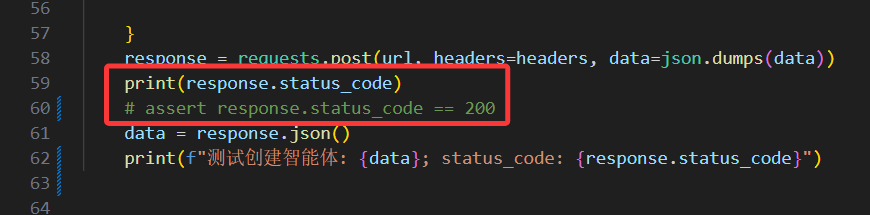
\includegraphics[width=0.8\textwidth]{103/printlog.png}
  \caption{打日志的例子}
\end{figure}

这样我就知道了程序在执行到这里的时候,返回的不是预期的200,而是404。于是这让我顺藤摸瓜,排查可能会导致404的原因,最终发现是因为某个API的返回值发生了变化,导致程序无法正常运行。

这是打日志的一个典型例子。通过在代码中添加打印语句,我们可以快速定位问题所在,并进行修复。

\subsubsection{打断点}

在VS Code中,我们可以通过点击行号左侧的空白区域来设置断点。断点是调试过程中非常重要的工具,它可以让代码执行到特定的某行时暂停,从而查看当前的变量值和程序状态。

我们可以逐行执行代码,查看变量的变化,从而定位问题所在。

\begin{figure}[ht]
  \centering
  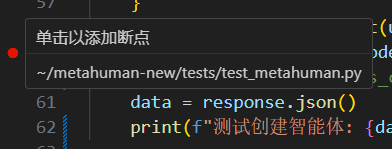
\includegraphics[width=0.8\textwidth]{103/breakpoints.png}
  \caption{打断点的例子}
\end{figure}

这样就可以打出一个断点。在调试过程中,当程序执行到断点所在的行时,程序会暂停,我们可以查看当前的变量值和程序状态。我们可以通过单步执行(Step Over)来逐行执行代码,或者通过单步进入(Step Into)来进入函数内部进行调试。对于小型项目或者单文件项目,打断点是一个非常有效的调试手段。

\subsubsection{写测试代码}

写测试代码是指编写一些专门用于测试的代码,以便在运行时验证程序的正确性。测试代码可以帮助我们发现潜在的问题,并确保程序的功能正常。这也是用于较大型项目的调试手段,但是小型项目也可以使用。我们可以在这些测试代码中模拟各种可能出现的情况(包括常规值、边界值、异常值等),从而验证程序的正确性和健壮性。

\begin{figure}[ht]
  \centering
  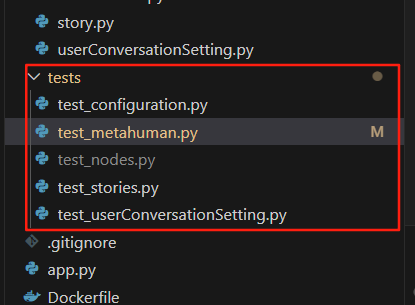
\includegraphics[width=0.8\textwidth]{103/tests.png}
  \caption{我为本人实习的项目编写的集成测试}
\end{figure}

\subsubsection{小结}

debug 最重要的一件事是缩小错误出现的范围,为达成这一目的我们通常会跟踪代码的行为,直到发现代码的行为与预期不符。实际上最棘手的情况是,代码只在特定的数据上出现错误,尤其是当我们无法获取程序执行日志的时候。这种情况尤见于我们在POJ上做题的时候:POJ的测试数据是不可见的,只会告诉你结果是WA、RTE还是TLE、MLE。

这时最应该做的是重新审视自己的预期(以及 OJ 题的题面),寻找是否遗漏了什么约束条件或关键信息。一份貌似运行正常的代码很有可能会在边界条件或复杂数据的情况下出问题,可以尝试手写一些处于边界条件之下的数据,或编写一个数据生成器来生成更复杂的数据。实在手足无措时,休息一下放空大脑也是很好的选择。实在走投无路之时,摇人求助也不是什么大不了的事情。debug 很可能会占用比编写代码更多的时间和精力,保持良好的心态才是 debug 的关键。

\section{Git与版本控制}

试想以下环境:我们正在写一项作业,开发工作已经基本完成,试运行也能够得到90分。此时我们希望进一步精进代码,使得分数达到95分以上;但是经过一通修改以后,发现程序再也运行不起来了。这时候距离ddl只有1小时,我们决定摆烂,提交能够得到90分的代码。然后我们根据记忆改回原来的代码的时候,发现我们再也想不起来旧代码是怎么写的了!这无疑是令人极为懊恼的。

再试想另一个环境:假设我们正在开发一个大型项目,项目中有很多人参与开发。如果使用传统的方式来分发代码,那么每个人都要手动下载代码,修改代码,然后再上传代码。这时候就会出现很多问题,例如代码冲突、版本不一致等。那这就需要专门的一个人或者几个人来管理代码的版本和分发,但是这样就会显著增加工作量和复杂度。

为了避免以上问题,我们引入了版本控制(VCS)系统。一般来说,VCS系统可以分为两类:集中式版本控制系统(CVCS,也叫中心化的)和分布式版本控制系统(DVCS,也叫去中心化的)。集中式版本控制系统的特点是所有的代码都存储在一个中心服务器上,所有的开发者都需要从中心服务器上下载代码,然后再上传代码;而分布式版本控制系统的特点是每个开发者都有一份完整的代码库,所有的操作都是在本地进行的,然后再将修改推送到中心服务器上。这样就可以避免代码冲突、版本不一致等问题。

2002 年以前,Linux 内核开发完全依赖于 Linus 一个人手工检查并合并全世界发来的补丁,这样工作量非常大。于是,Linus 的一个朋友介绍了 BitMover 公司开发的商业 VCS 软件 BitKeeper 免费授权给 Linux 开发团队使用。此举招致了 FSF 的 RMS 等人的批评,认为在自由软件开发中使用非自由软件是“道德上有污点”的行为。但是作为实用主义者的 Linus 并不在意这些事情,BitKeeper 作为去中心化的 VCS,满足了 Linus 的需求。然而好景不长,有 Linux 内核开发者逆向了 BitKeeper 的协议,致使 BitMover 公司在 2005 年决定收回其授权。Git 就是在这种条件下诞生的,据说第一版 Git 是 Linus 利用 1 周休假时间完成的。随着Linux的广泛应用,Git也逐渐成为了最流行的去中心化版本控制系统,也是目前最流行的版本控制系统。

\begin{figure}[ht]
  \centering
  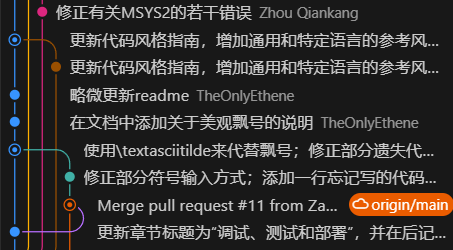
\includegraphics[width=0.8\textwidth]{103/git.png}
  \caption{一个典型的Git工作流程}
  \label{fig:git-workflow}
\end{figure}

\subsection{Git的工作原理}

Git有三个目录共同完成版本控制:工作区、暂存区、版本库。工作区是项目目录,暂存区是一个隐藏的文件夹.git,版本库是一个隐藏的文件夹.git/objects。工作区是我们平时使用的目录,暂存区是Git用来存储修改的地方,版本库是Git用来存储所有版本信息的地方。版本库有一个指针,指向当前版本的某一节点(一般指向最新的节点)。每个节点都有一个唯一的哈希值\footnote{哈希(Hash,也叫散列)指的是固定长度、像指纹一样的唯一小串字符,可用于快速校验、查找或加密等功能。},用来标识该节点。每个节点包含了该版本的所有文件和目录的信息,以及指向上一个版本的指针。Git使用哈希值来标识每个版本,这样可以保证每个版本都是唯一的。

这样讲解很难以理解,我们不妨举例说明:现在,Git中有一个版本为X的节点,包括文件A和文件B两个文件。这些文件存储在版本库中。此时,工作区为空,暂存区为空,指针指向X。我现在希望对它们进行修改,这个修改遵循以下过程:

\begin{enumerate}
  \item 我拿出了这些文件,并且对文件A进行修改。此时,工作区有AB两个文件,但是暂存区依然是空的。我们的任何修改都不会被暂存区记录,Git也不会知道我对这些文件进行了修改。

  \item 我觉得修改差不多了,现在把A放进暂存区。现在Git知道我对A进行了一些修改了。
    \begin{figure}[ht]
      \begin{subfigure}[t]{0.45\linewidth}
        \centering
        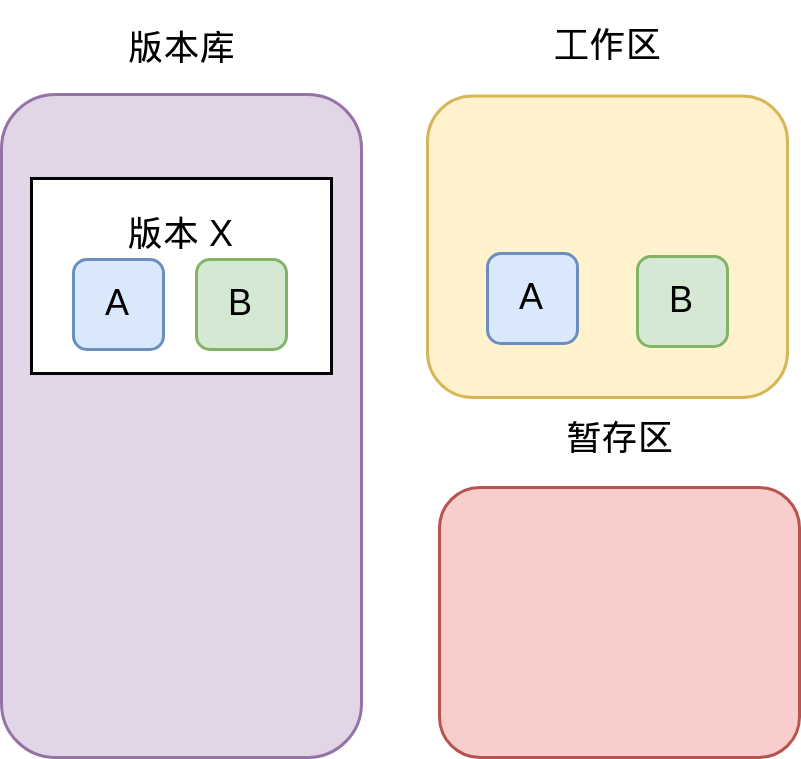
\includegraphics[width=\linewidth]{103/git-graph-no-modified.png}
      \end{subfigure}
      \hfill               % 把左右撑开
      %----- 右图 -----
      \begin{subfigure}[t]{0.45\linewidth}
        \centering
        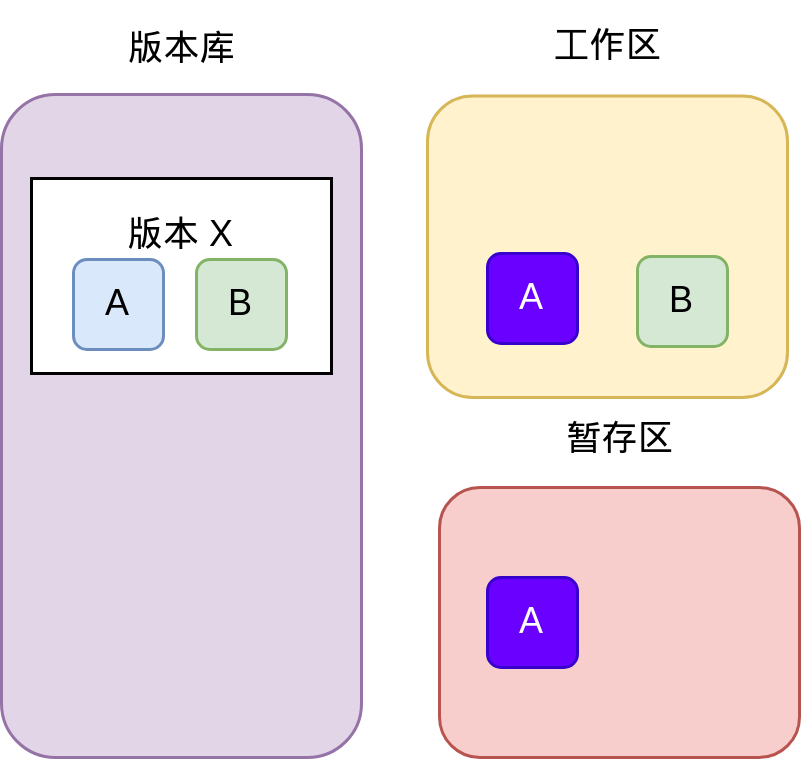
\includegraphics[width=\linewidth]{103/git-a-changed.png}
      \end{subfigure}
    \end{figure}
  \item 我又对B进行了类似的修改,此时B也进暂存区了。
  \item 我觉得修改差不多了。我认为我应该永久保存目前的状态,于是就把暂存区提交到版本库。此时版本库多了一个Y节点,指针也指向Y节点,有修改过的AB两个文件。此时,暂存区又清空了,而工作区和版本库的Y版本一致。
    \begin{figure}[ht]
      \begin{subfigure}[t]{0.45\linewidth}
        \centering
        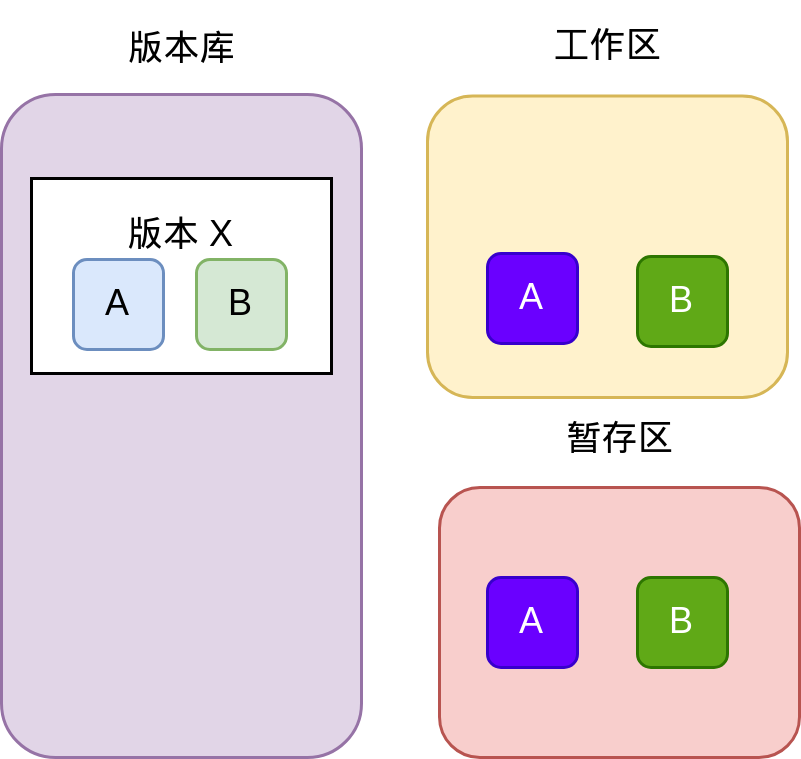
\includegraphics[width=\linewidth]{103/git-b-changed.png}
      \end{subfigure}
      \hfill               % 把左右撑开
      %----- 右图 -----
      \begin{subfigure}[t]{0.45\linewidth}
        \centering
        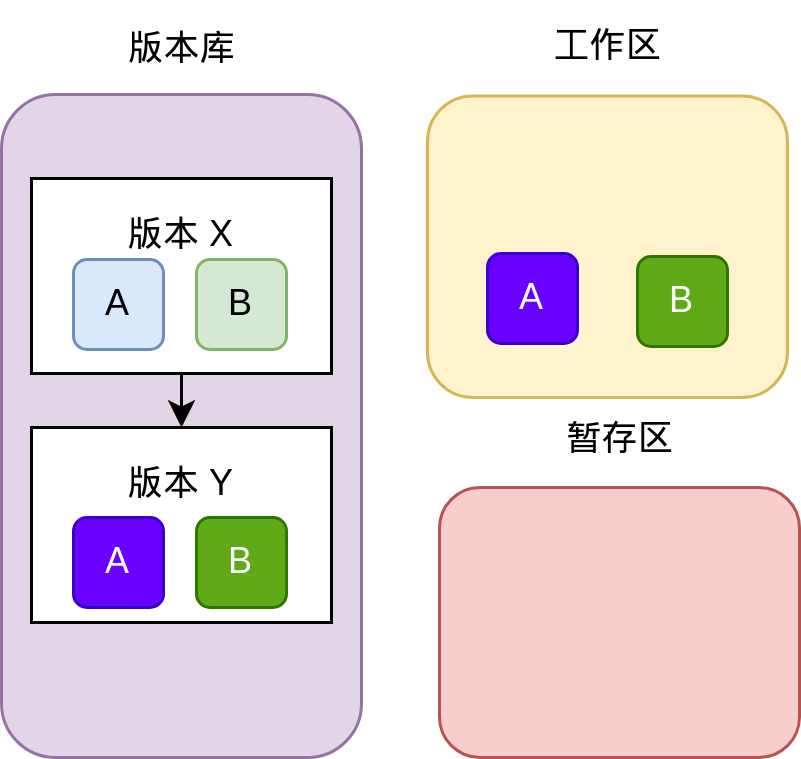
\includegraphics[width=\linewidth]{103/git-commited.png}
      \end{subfigure}
    \end{figure}
\end{enumerate}

\subsection{下载Git}

一个最简单的方式是使用Winget包管理器:

\begin{lstlisting}[language=bash]
    winget install Microsoft.git
\end{lstlisting}

或者你也可以从官方网站上下载并安装之。同样,安装的时候一定要勾选“添加到PATH”这一选项,否则你在命令行中无法使用Git。

\subsection{Git信息设置}

安装并使用Git的第一步是先编辑本地的一些信息。Git的提交需要一个用户名和一个邮箱,来对应每次提交的作者。我们可以使用以下命令来设置这些信息:

\begin{lstlisting}[language=bash]
    git config --global user.name "Your Name"
    git config --global user.email "email@example.com"
\end{lstlisting}

这样即可设置全局用户名和邮箱。如希望给某个特定仓库设置特定的用户名和邮箱,你需要在该仓库下重新执行上述命令,但是不写--global命令。

现代Git一般提倡使用main作为根分支的名称。而Git依然使用旧的master分支作为根分支,你可以使用以下命令修改为main:

\begin{lstlisting}[language=bash]
    git config --global init.defaultBranch main
    # 这条命令会修改全局的默认分支名称
\end{lstlisting}

\subsection{Git的最基本使用}

\subsubsection{提交}

要具体地在某一目录下进行版本控制,我们需要在命令行中进入到我们希望使用Git的目录下。然后我们可以使用以下命令来初始化一个Git仓库:

\begin{lstlisting}[language=bash]
    git init
\end{lstlisting}

如果你在视窗中开启了“显示隐藏文件”这类功能,你就会发现一个隐藏的文件夹.git出现在了你当前的目录下。这个文件夹就是Git用来存储版本信息的地方。

然后你可以使用以下命令来添加文件到Git仓库中(这个命令的实际意义是把文件添加到暂存区);

\begin{lstlisting}[language=bash]
    git add <filename>
\end{lstlisting}

如果我们忘记了当前状态下有哪些文件被修改了,我们可以使用以下命令来查看当前状态:
\begin{lstlisting}[language=bash]
    git status
\end{lstlisting}

如果你觉得修改差不多了,保存文件以后,你可以使用以下命令来提交文件到Git仓库中(这个命令的实际意义是把暂存区的文件提交到版本库中):

\begin{lstlisting}[language=bash]
    git commit -m "commit message"
\end{lstlisting}

上述内容中,-m后面是提交信息。提交信息是对本次提交的简要描述。我们建议每次提交都写上简要的提交信息,这样可以帮助我们更好地理解代码的修改历史。

\subsubsection{回退}

如果出现了先前我们说的不小心写坏了的情况,这时候就可以进行版本回退了。我们可以使用以下命令来查看当前的版本信息:

\begin{lstlisting}[language=bash]
    git log # 例如版本库是a-b-c-d-e-f-g
\end{lstlisting}

找到你希望回退到的版本的哈希值(前几位即可),然后使用以下命令来回退到该版本(这个命令会把指针回退到指定的版本,丢弃之后的所有内容,然后丢弃暂存区和工作区的所有东西):

\begin{lstlisting}[language=bash]
    git reset --hard <commit_hash>
    # 请谨慎使用这一命令!该命令不会保留当前的修改!
\end{lstlisting}

如果你希望回退到某个版本,但是不想丢失当前的修改,你可以使用以下命令来回退到该版本(这个命令会把版本库后面的东西全部丢弃,清空暂存区,但是保留当前工作区):
\begin{lstlisting}[language=bash]
    git reset --mixed <commit_hash>
    # 我们更加推荐这个回退方式,--mixed可以省略,或者用--soft替代。
    # 用--soft替代时,不会清空暂存区。
\end{lstlisting}

使用图解来表示一下:
\begin{figure}[ht]
  \centering
  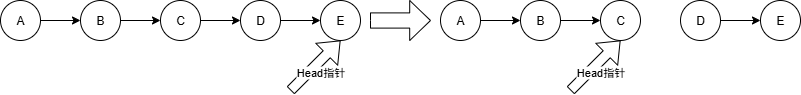
\includegraphics[width=0.8\textwidth]{103/git-reset.png}
  \caption{Git的回退操作}
  \label{fig:git-reset}
\end{figure}
可以看到,回退操作虽然会把指针回退到指定的版本并丢弃之后的版本,但是之后的版本提交依然存在于版本库中,只是被从树上摘下来了。这些提交被称为“孤立提交”。如果希望恢复或者删除这些孤立提交,可以执行以下命令:
\begin{lstlisting}[language=bash]
    git fsck --lost-found # 查看孤立提交、孤立分支等
    git checkout <commit_hash> # 进入分离头模式
    git branch <branch_name> # 创建一个分支来恢复孤立提交

    git gc --prune=now # 清理孤立提交
\end{lstlisting}
即使我们不使用\texttt{git gc}手动清理孤立提交,随着时间的推移(一般是90天提交记录过期),孤立提交也会被Git逐渐自动清理掉。

\subsubsection{排除相关文件}

有时候我们版本跟踪的时候不需要跟踪一些文件,例如具有敏感信息的文件(如密码),或者构建文件等。此时,我们可以创建一个文件 .gitignore 来阻止跟踪。例如,在Linux下,构建文件往往是*.o。那么我们可以在上述文件中加入 *.o ,之后git就会忽略这些文件。

\subsection{分支管理}

有时候我们想同时开发新功能,并且调优以前的代码,这样可能就需要两条线进行开发。这时,分支相关的功能就会很有帮助。Git 的分支功能允许我们在同一个仓库中创建多个独立的开发线,每个分支可以独立地进行提交和修改。

我们可以做如下假设:已经有一个名为main的分支,并已经有了一列提交记录A、B、C。现在,我希望开发一个新的功能,但是不想影响到main分支上的代码。这时,我们可以创建一个新的分支,例如feature,并在该分支上进行开发。

\subsubsection{创建和切换分支}

可以使用以下命令创建一个新的分支并切换到该分支:
\begin{lstlisting}[language=bash]
git checkout -b feature
\end{lstlisting}

以上等价于执行
\begin{lstlisting}[language=bash]
git branch feature <commit-hash of C>
git checkout feature
\end{lstlisting}

如果我现在想要回到main分支,可以使用以下命令:
\begin{lstlisting}[language=bash]
git checkout main
\end{lstlisting}

\subsubsection{分支变基}

如果我们已经在feature分支上进行了多次提交F、G,同时在main分支上也有了新的提交D、E。现在想要将feature这些提交变基到main分支上,可以使用以下命令:
\begin{lstlisting}[language=bash]
  git rebase main
  git checkout main
\end{lstlisting}
这样会把上述feature上的三个提交从C变基到E,变成F'和G'。我们可以用图解来理解这个过程:

\begin{figure}[ht]
  \centering
  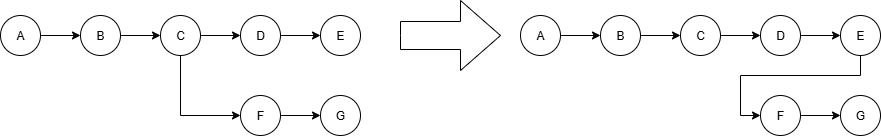
\includegraphics[width=\textwidth]{103/git-rebase.png}
  \caption{分支变基示意图}
  \label{fig:git-rebase}
\end{figure}

变基操作会改变提交的哈希值。

\subsubsection{合并分支和冲突解决}

如果我们想要将feature分支上的代码合并(不是变基)到main分支上,可以使用以下命令:

\begin{lstlisting}[language=bash]
git checkout main
git merge feature
\end{lstlisting}

这时候我们在main分支上,并试图将E和G合并在一起。这时,会自动创建一个特殊的提交Merge,它有两个父提交。之后的提交就会以Merge为父提交,而不是E或G中的任何一个。

\begin{figure}[ht]
  \centering
  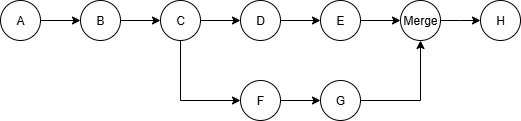
\includegraphics[width=0.75\textwidth]{103/git-merge.png}
  \caption{分支合并示意图}
  \label{fig:git-merge}
\end{figure}

如果这两个提交没有冲突,那么合并会自动完成。但是如果有冲突(例如两个分支涉及到同一行的修改),Git 会提示我们解决冲突。此时,我们不得不手动解决冲突。我们会看到以下内容(或者其英文版本):
\begin{lstlisting}[language=bash]
  自动合并 example1.txt
冲突(内容):合并冲突于 example1.txt
自动合并失败,修正冲突然后提交修正的结果。
\end{lstlisting}
此时,我们需要打开冲突的文件,手动解决冲突。Git 会在冲突的地方插入标记,例如:
\begin{lstlisting}[language=bash]
  <<<<<<< HEAD
  这是 main 分支上的内容。
  =======
  这是 feature 分支上的内容。
  >>>>>>> feature
\end{lstlisting}
我们需要手动编辑这个文件,删除这些标记,并保留我们想要的内容。

如果使用Code等编辑器,通常会有冲突解决的工具,可以帮助我们更方便地解决冲突。

解决完冲突后,我们需要使用以下命令来标记冲突已解决:
\begin{lstlisting}[language=bash]
  git add .
  git merge --continue
\end{lstlisting}

\subsubsection{删除分支}

如果我们已经完成了feature分支上的开发,并且已经将其合并到main分支上,可以使用以下命令删除该分支:
\begin{lstlisting}[language=bash]
git branch -d feature
\end{lstlisting}

一般不建议直接删除分支,而是使用 \texttt{-d} 选项来删除已经合并的分支。如果分支没有被合并,可以使用 \texttt{-D} 选项强制删除。

\subsubsection{压缩提交}

有时候,我们在开发过程中,可能会有很多小的提交,这些提交可能是一些临时的修改或者调试信息。为了保持代码和版本库的整洁,我们可以使用 Git 的压缩提交功能,将多个提交合并为一个提交。这个压缩功能被称作是\textbf{Squash},但是特别注意:没有\texttt{git squash}命令。

我们一般只在分支合并的时候使用压缩提交。可以使用以下命令中的一个来压缩提交:
\begin{lstlisting}[language=bash]
git merge --squash feature
\end{lstlisting}

\subsection{标签管理}
标签(Tag)是 Git 中用于标记特定提交的功能。标签通常用于标记版本发布或重要的里程碑。与分支不同,标签是静态的,不会随着提交而移动。

\subsubsection{创建标签}
可以使用以下命令创建一个标签:
\begin{lstlisting}[language=bash]
git tag v1.0
\end{lstlisting}

这将创建一个名为 v1.0 的标签,指向当前的提交。如果需要为特定的提交创建标签,可以在命令中指定提交的哈希值:
\begin{lstlisting}[language=bash]
git tag v1.0 <commit-hash>
\end{lstlisting}

\subsubsection{查看标签}
可以使用以下命令查看所有标签:
\begin{lstlisting}[language=bash]
git tag
\end{lstlisting}

\subsubsection{删除标签}
如果需要删除一个标签,可以使用以下命令:
\begin{lstlisting}[language=bash]
git tag -d v1.0
\end{lstlisting}

\subsection{“摘樱桃”}

Cherry-Pick(摘樱桃)操作(也叫挑拣)是指从一些提交中选择一些特定的提交(修改),并将这些提交(修改)应用到当前分支上。这适用于当我们只想要一些特定的提交而不是整个分支的所有提交的时候。

一般,CherryPick操作很难使用命令行来操作,其复杂程度过高。我们可以使用VS Code的自带Git视窗或者GitLens等工具来进行这个操作。

使用视窗进行挑拣非常方便,我们只需要在提交列表中选择需要的提交,然后右键点击“Cherry-Pick”(汉化应该是挑拣)即可。这样会将选中的提交应用到当前分支上。

\section{GitHub与多人协作}

\subsection{远程仓库}

很多项目无法只在一台机器上进行开发,往往都需要在远程部署一个仓库(例如GitHub、GitLab等,或者公司自建库),然后将本地的代码推送到远程仓库中。这样,我们就可以在不同的机器上从远程仓库中拉取代码,从而保证代码的一致性。

在本节,我们将使用 GitHub 作为远程仓库的示例,介绍如何将本地仓库与远程仓库进行关联、推送和拉取代码。

\subsubsection{创建仓库}
首先,我们需要在 GitHub 上创建一个新的仓库。创建完成后,GitHub 会提供一个远程仓库的 URL,例如:
\begin{lstlisting}
  https://github.com/YourName/example.git
\end{lstlisting}
我们可以在GitHub上的仓库页面中找到这个 URL,如图所示。

\begin{figure}[ht]
  \centering
  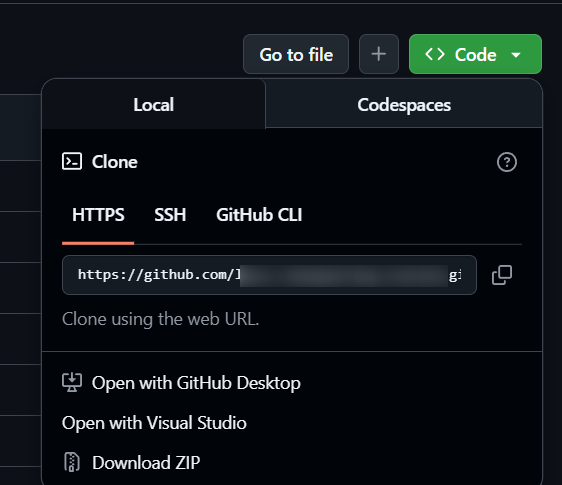
\includegraphics[width=0.5\textwidth]{103/example.png}
  \caption{GitHub 上的仓库页面}
  \label{fig:github-repo}
\end{figure}

接下来,我们需要将本地仓库与远程仓库关联。可以使用以下命令:
\begin{lstlisting}[language=bash]
git remote add origin <your-repo-url>
\end{lstlisting}
这将把远程仓库的 URL 添加为名为 origin 的远程仓库。origin 是习惯上的远程仓库名称。

现在我们要将这个本地仓库的代码推送到远程仓库中。可以使用以下命令:
\begin{lstlisting}[language=bash]
git push -u origin main
\end{lstlisting}
这里的 \texttt{-u} 选项表示将本地的 main 分支与远程的 main 分支关联起来,以后可以直接使用 \texttt{git push} 和 \texttt{git pull} 命令进行推送和拉取。

如果本地分支名称和远程有区别,(例如本地仓库主要分支是master,而远程仓库的主要分支是main),我们可以使用以下命令来推送代码:
\begin{lstlisting}[language=bash]
git push -u origin master:main
\end{lstlisting}
这将把本地的 master 分支推送到远程的 main 分支。

\subsubsection{使用仓库}

如果你是仓库的使用者,想要从远程仓库中拉取代码(但是本地没有这个仓库),可以使用以下命令:

\begin{lstlisting}[language=bash]
git clone <your-repo-url>
\end{lstlisting}

这样会在本地创建一个\textbf{新的}目录,并将远程仓库的代码克隆到该目录中。在克隆代码的时候,Git 会自动创建与远程同名的分支,并把它们与远程的 main 分支关联起来。

如果你已经有了本地仓库,并且想要将远程仓库的代码拉取到本地,经典的操作是以下命令:
\begin{lstlisting}[language=bash]
git pull origin main
\end{lstlisting}
直接使用 \texttt{git pull} 命令也是可以的,因为我们之前已经使用 \texttt{-u} 选项将本地分支与远程分支关联起来了。然而,需要注意的是现代的拉取操作往往不推荐使用 \texttt{git pull} 命令,因为它会自动合并远程分支的代码到本地分支,这可能会导致冲突。更推荐的做法是先使用 \texttt{git fetch} 命令拉取远程仓库的代码,然后再手动合并:
\begin{lstlisting}[language=bash]
git fetch origin
git merge origin/main
\end{lstlisting}
这样可以更好地控制合并过程,避免自动合并带来的问题。

如果你在本地做出了一些修改,想要将这些修改推送到远程仓库,可以使用以下命令:
\begin{lstlisting}[language=bash]
git push origin main
\end{lstlisting}
直接使用 \texttt{git push} 命令也可以。

如果存在某些提交在远程仓库中,而本地仓库没有这些提交,Git 会提示你先拉取远程仓库的代码,然后再推送本地的修改。这是因为 Git 不允许直接推送到远程仓库,除非本地仓库是最新的。如果你确定你不需要远程仓库的提交,可以使用以下命令强制推送本地的修改:
\begin{lstlisting}[language=bash]
git push -f origin main
\end{lstlisting}

\begin{warning}
  强制推送会覆盖远程仓库的代码,可能会导致其他工作丢失,因此请谨慎使用。
\end{warning}

\subsection{GitHub界面指南}

我们打开GitHub的一个仓库的时候,映入眼帘的类似这张图片内容。可以看到,这些图片中有很多不同的概念和功能。我们来逐一介绍一下。

\begin{figure}[ht]
  \centering
  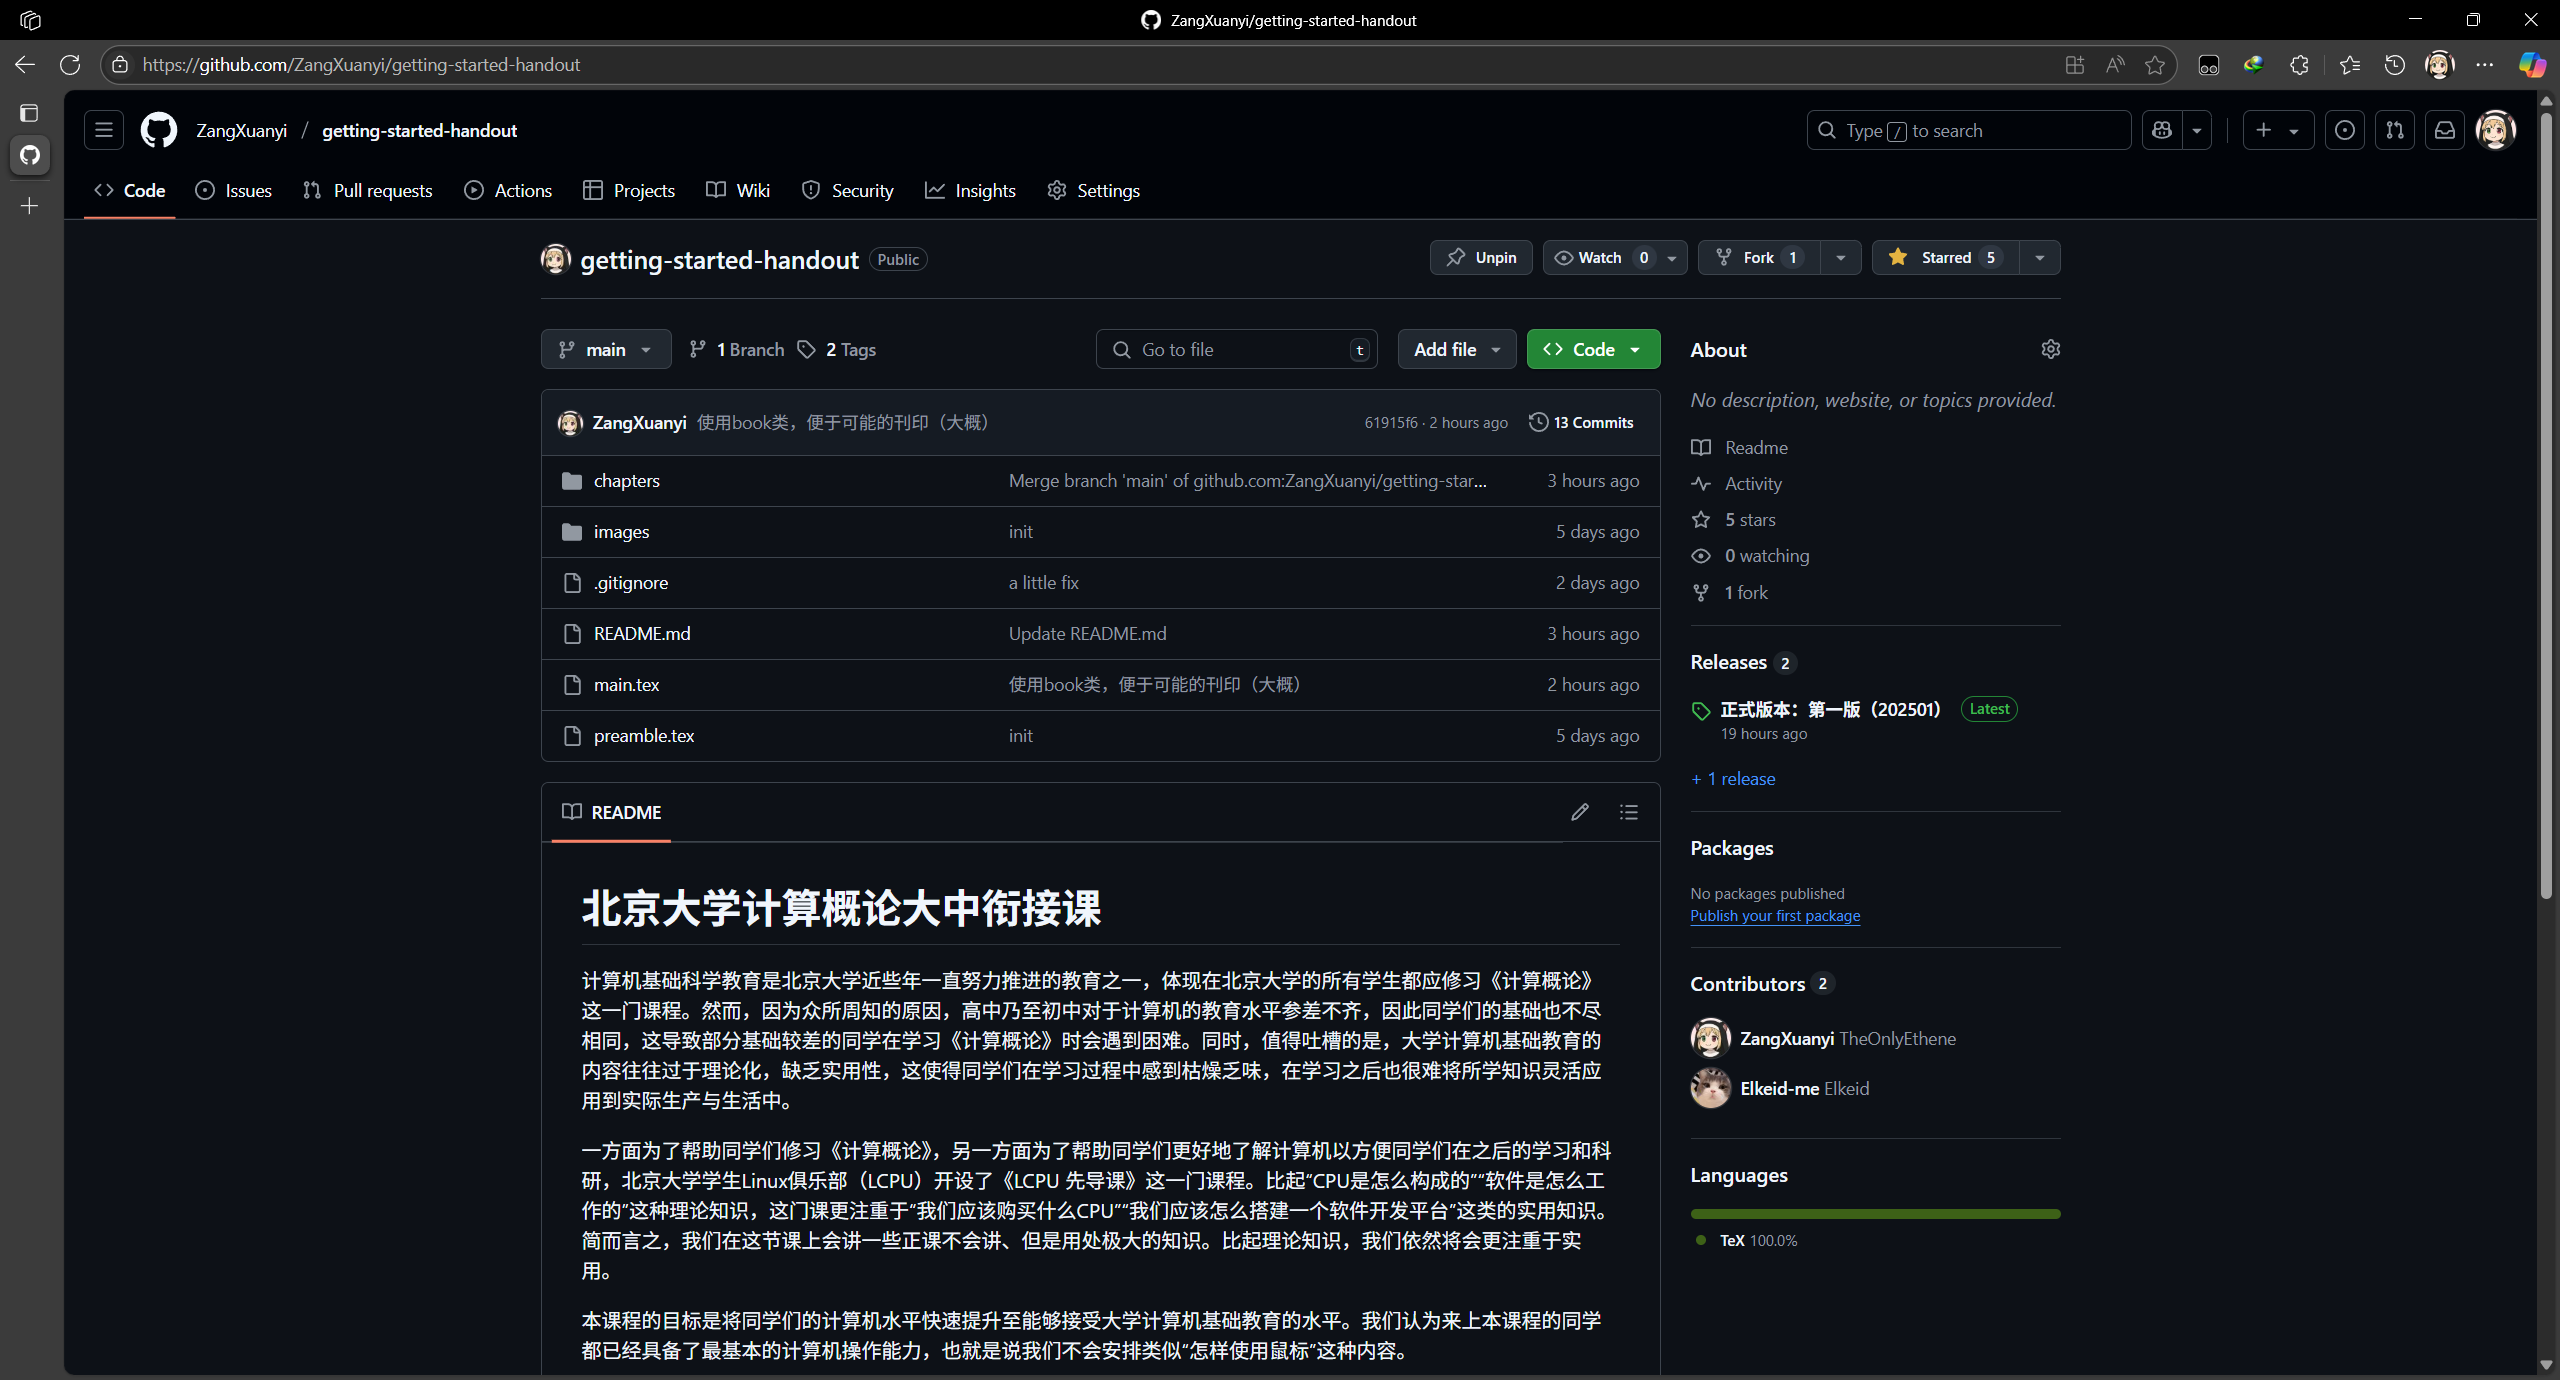
\includegraphics[width=\textwidth]{103/github.png}
  \caption{GitHub 仓库页面}
  \label{fig:github}
\end{figure}

在上面的一栏中,我们可以看到以code、issues、pull requests等为标题的选项卡。每个选项卡对应着一个功能模块。

\begin{itemize}
  \item \textbf{Code}:代码模块,显示仓库中的代码文件和目录结构。我们可以在这里浏览代码、下载代码、查看提交历史等。
  \item \textbf{Issues}:问题模块,用于跟踪和管理项目中的问题和任务。我们可以在这里创建新的问题、查看已有的问题、评论和解决问题等。在Gitea上,问题模块被称为“工单”(Tasks),这与它常用于公司自建库的特点有关。
  \item \textbf{Pull Requests}:合并请求模块,用于管理代码的合并和审查。我们可以在这里创建新的合并请求、查看已有的合并请求、评论和审查代码等。Pull Request(简称 PR)是 GitHub 和 GitLab 等平台提供的一种代码审查和合并的机制,具体内容可以参考\ref{sec:pull-request}节。
  \item \textbf{Actions}:自动化模块,用于管理项目的自动化工作流。我们可以在这里创建新的工作流、查看已有的工作流、运行和调试工作流等。
  \item \textbf{Projects}:项目模块,用于管理项目的进度和任务。我们可以在这里创建新的项目、查看已有的项目、添加任务和卡片等。
  \item \textbf{Wiki}:维基模块,用于管理项目的文档和知识库。我们可以在这里创建新的页面、编辑已有的页面、添加图片和链接等。GitHub Wiki 是 GitHub 提供的一种文档管理工具,可以帮助我们编写和维护项目的说明文档。
  \item \textbf{Security}:安全模块,用于管理项目的安全性和漏洞。我们可以在这里查看项目的安全报告、修复漏洞、配置安全策略等。
  \item \textbf{Insights}:洞察模块,用于分析项目的活动情况,例如提交历史、问题和合并请求的统计信息等。我们可以在这里查看项目的活跃度、贡献者的统计信息、代码的质量和覆盖率等。
  \item \textbf{Settings}:设置模块,用于管理项目的设置和配置。我们可以在这里修改项目的名称、描述、权限等属性。
\end{itemize}

靠下一行就是仓库的名称,右面是仓库的描述和一些操作按钮。Star 用来标记喜欢的仓库,Fork 用来复制仓库到自己的账户下,Watch 用来关注仓库的更新。

再靠下一行,我们可以看到仓库的分支(Branch)和提交(Commit)信息。分支是代码的不同版本,提交是代码的历史记录。我们可以在这里切换分支、查看提交历史、比较不同分支的差异等。同一行的那个绿色的Code按钮是用来下载代码的,可以选择下载为 ZIP 文件或者使用 Git 克隆仓库。我们非常推荐使用 Git 克隆仓库,因为这样可以更方便地管理代码和提交。

页面的左下方部分,在文件目录之下,是仓库的readme文件内容。README 文件是仓库的说明文档,通常包含项目的介绍、安装和使用说明、贡献指南等信息。我们可以在这里查看项目的详细信息。

页面右侧的一列是仓库的统计信息,包括提交历史、分支、标签、贡献者等。我们可以在这里查看项目的活跃度、贡献者的统计信息、代码的质量和覆盖率等。同时,我们也可以在这里找到仓库的发行版等信息。

\subsection{多人协作}

成熟的项目往往是由多人协作完成的,因此需要一些规范来管理代码的提交和合并等。GitHub、GitLab等提供了多种方式来支持多人协作,包括分支管理、代码审查、合并请求等。

\subsubsection{Fork}

Fork 是 GitHub 和 GitLab 等平台提供的一种代码复制和协作的机制。它允许用户将其他人的仓库复制到自己的账户下,从而可以在自己的仓库中进行修改和提交。这样可以使得修改更加方便(主要是防止权限不够),并且可以避免直接修改原仓库的代码。当然,权限足够的情况下,我们往往会直接在原仓库中创建新分支进行修改。

\subsubsection{Pull Request}\label{sec:pull-request}
Pull Request(简称 PR)是 GitHub 和 GitLab 等平台提供的一种代码审查和合并的机制。它允许开发者在完成某个功能或修复某个问题后,将自己的代码提交到主分支(通常是 main 或 master)之前,先进行代码审查和讨论。

PR 的工作流程通常如下:

\begin{enumerate}
  \item 开发者fork(分叉)一个仓库,或者在原仓库中创建一个新的分支。
  \item 开发者在自己的分支上进行开发,完成某个功能或修复某个问题。
  \item 创建一个PR,请求将自己的分支合并到主分支。PR 中可以包含对代码的描述、相关问题的链接等信息。
  \item 其他开发者可以对 PR 进行代码审查,提出修改意见或建议。
  \item 开发者根据审查意见修改代码,并更新 PR。
  \item 当 PR 获得足够的审查和批准后,可以将其合并到主分支。通常会有一个维护者或项目负责人来执行这个操作。
  \item 合并后,PR 会被关闭,相关的分支可以被删除;也可以保留,以便后续的开发和维护。
\end{enumerate}

\subsubsection{Lint}

在多人协作中,代码风格和规范的一致性非常重要。Lint 工具可以帮助我们检查代码中的潜在问题和不符合规范的地方。常见的 Lint 工具有 ESLint(用于 JavaScript)、Pylint(用于 Python)等。

如果我们在仓库中包含了 Lint 工具的配置文件(例如 .eslintrc.json 或 .pylintrc),那么在提交代码时,Git 会自动运行 Lint 工具,对代码进行检查。如果代码不符合规范,Lint 工具会给出相应的错误或警告信息。

Lint 工具通常会在 PR 中自动运行,并将检查结果反馈给开发者。开发者可以根据检查结果修改代码,确保代码符合项目的规范。

\subsubsection{成熟项目的分支管理策略}

在成熟的项目中,一般会采用一些分支管理策略来规范分支的使用和合并等。一般说来,同一个仓库中会有以下几种分支:(以下是Git Flow的工作管理策略)
\begin{itemize}
  \item main/master:主分支,通常是代码的稳定版本。一般禁止直接提交代码,只能通过合并其他分支来进行更改。
  \item develop/dev:开发分支,一般是集成了所有的新功能的基准分支,是开发的主要分支。该分支从main分出,最终也要进入main分支。对于一些较为轻量级的项目,有时候会直接使用feature分支来代替develop分支。
  \item feature/\textit{feature-name}:功能分支,每个新功能或改进都在独立的分支上进行开发。不同的开发者可以在不同的功能分支上工作,完成后再合并到develop分支。在功能完成开发后,通常会删除该分支。
  \item hotfix/\textit{hotfix-name}:热修复分支,一般是绕过开发流程,直接从main分支分出,修复完成后再合并回main分支和develop分支。热修复分支通常用于修复生产环境中的紧急问题,在问题彻底解决之后,该分支往往会被删除。
  \item release/\textit{release-name}:发布分支,一般用于准备发布新版本的代码。该分支从develop分出,经过测试和修复后再合并回main分支和develop分支。发布分支通常用于准备发布新版本的代码。在发布完成后,通常会删除该分支。不过现在往往会直接使用打标签的方式来替代发布分支。
\end{itemize}

开发的一般流程是:在main分支上发布了第一个稳定的版本后,会分出一个dev分支。之后,通常会禁止大多数人对main进行直接提交或者合并,所有新功能都在dev分支上开发,具体的形式是从dev分支上分出多个feature分支来进行多线、多功能的同时开发,且对于大型项目,dev分支往往也只允许合并,禁止小的提交。

有时候合并进dev分支的代码可能存在一些问题,而测试和检查又疏忽,导致合并进main分支之后出现了错误。此时,我们需要直接从main分支分出一个hotfix分支来修复问题,可能会采用一些临时的策略来修复问题。修复完成后,hotfix分支会被合并回main分支。在这之后,main分支会被合并进dev分支以同步代码,然后对hotfix分支上出现的问题加以更稳定的修复。在修复完成后,再将dev分支合并进main分支,此时可以删除hotfix分支。

除了Git Flow,还有其他一些分支管理策略,例如GitHub Flow、GitLab Flow等。GitHub Flow 是 GitHub 提出的分支管理策略,主要用于快速迭代和持续集成,其开发非常轻量级,一般只有 main/master 和 feature 分支。GitLab Flow 则是 GitLab 提出的分支管理策略,多出了产品分支和预发布分支等,分别用于生产环境和预发布环境。

\section{密钥与远程}

在初阶课程中,我们已经知道了密钥是什么东西,并且知道了在大多数的情况下要使用密钥而不是密码来进行身份验证。但是关于“怎么使用和管理”密钥,则没有进行详细介绍。在本节中,我将会详细地介绍密钥的使用和管理。

密钥是一种加密技术,用于保护数据的安全性和完整性。密钥的设计通常基于非常困难的数学问题,例如大数分解、椭圆曲线等。密钥通常分为两种类型:对称密钥和非对称密钥。对称密钥使用相同的密钥进行加密和解密,可以理解为家里的每一个人都使用同一把钥匙来开门,如果钥匙丢了(密钥泄漏)则加密的数据就不再安全。非对称密钥使用一对密钥进行加密和解密,通常称为公钥和私钥,可以理解为旧式邮箱,所有人都可以往信箱里投信(公钥),但是只有邮递员(私钥)可以打开信箱取信。非对称密钥的安全性更高,因为即使公钥泄漏,私钥依然是安全的。

现代加密技术往往使用混合加密方式,即使用非对称密钥来交换对称密钥,然后使用对称密钥来加密数据。这样可以兼顾安全性和效率。

对于个人而言,最常用的加密方式是以SSH为代表的非对称密钥加密方式。SSH(Secure Shell)是一种网络协议,用于在不安全的网络上进行安全的远程登录和其他网络服务。SSH 使用非对称密钥加密技术来保护数据的安全性和完整性。

\subsection{SSH密钥的生成}

在Windows上,我们需要安装系统功能OpenSSH Client来进行密钥的初步使用。在Linux和Mac上,OpenSSH通常是预装的。如果没有安装,请自行查找相关资料进行安装。

在安装完成后,我们可以使用以下命令来生成密钥对:
\begin{lstlisting}[language=bash]
ssh-keygen -t rsa -b 4096 -C "<你的邮箱地址>"
\end{lstlisting}

上述命令会生成一个 RSA 密钥对,密钥长度为 4096 位,并且会在密钥中添加一个注释(通常是你的邮箱地址)。执行该命令后,会提示你输入密钥的保存路径和密码。默认情况下,密钥对会保存在 \texttt{\textasciitilde/.ssh/id\_rsa} 和 \texttt{\textasciitilde/.ssh/id\_rsa.pub} 中。

RSA密钥对是最常用的密钥对之一,不过因为 RSA 密钥对的安全性已经不如以前了,因此现在推荐使用 Ed25519 密钥对。可以使用以下命令生成 Ed25519 密钥对:
\begin{lstlisting}[language=bash]
ssh-keygen -t ed25519 -C "<你的邮箱地址>"
\end{lstlisting}

生成密钥对后,我们需要将公钥(\texttt{id\_rsa.pub} 或 \texttt{id\_ed25519.pub})添加到远程服务器或服务(例如 GitHub、GitLab、CLab 等)的 SSH 密钥列表中。我们可以使用任何喜欢的编辑器打开上述公钥文件,复制其中的内容,并将其粘贴到指定的位置。\textbf{\color{red}同时,私钥(\texttt{id\_rsa} 或 \texttt{id\_ed25519})必须保密,绝对不能泄露给任何人!}

如果我们本地是Linux或者Mac且能够直接访问远程服务器,可以使用以下命令将公钥复制到远程服务器上:
\begin{lstlisting}[language=bash]
ssh-copy-id user@remote-server
\end{lstlisting}

我们也可以手动将公钥复制到远程服务器的 \texttt{\textasciitilde/.ssh/authorized\_keys} 文件中。我们可以使用记事本或者code等编辑器打开公钥文件,复制其中的内容,然后在远程服务器上使用以下命令将其添加到 \texttt{\textasciitilde/.ssh/authorized\_keys} 文件中。以上方法适用于无法使用 ssh-copy-id 命令的情况,例如Windows系统。

为了保护私钥的安全,我们可以为私钥设置一个密码。这样,在使用私钥进行身份验证时,需要输入密码才能解锁私钥。可以在生成密钥对时设置密码,也可以在后续使用 \texttt{ssh-keygen} 命令修改密码。

设置密码的方式非常简单。在生成密钥对时,系统会提示你输入密码。如果你不想设置密码,可以直接按 Enter 键跳过。

如果你已经生成了密钥对,但没有设置密码,可以使用以下命令为私钥设置密码:
\begin{lstlisting}[language=bash]
ssh-keygen -p -f ~/.ssh/id_rsa
\end{lstlisting}

实际上如果保密需求不是非常高的话,我们可以不设置密码。因为使用密钥除了安全性以外,最大的好处是可以免去每次连接远程服务器时输入密码的麻烦。而如果设置了密码,则每次连接远程服务器时都需要输入密码,这样就失去了使用密钥的便利性。

\subsection{密钥的使用}

在生成密钥对并将公钥添加到远程服务器或服务后,我们就可以使用密钥进行身份验证了。使用密钥进行身份验证的方式与使用密码类似,只不过需要指定私钥文件。

\subsubsection{连接到远程服务器}

可以使用以下命令连接到远程服务器:
\begin{lstlisting}[language=bash]
ssh -i ~/.ssh/id_rsa user@remote-server
\end{lstlisting}
如果你使用的是 Ed25519 密钥对,则需要将 \texttt{id\_rsa} 替换为 \texttt{id\_ed25519}。

如果你已经将私钥添加到 SSH Agent(实际上这确实是更一般的情况)中,可以直接使用以下命令连接到远程服务器:
\begin{lstlisting}[language=bash]
ssh user@remote-server
\end{lstlisting}

\subsubsection{Git托管}

GitHub的有两种托管代码的方式:HTTPS 和 SSH。HTTPS 是通过用户名和密码进行身份验证,而 SSH 是通过密钥进行身份验证。我们建议使用 SSH 进行身份验证,因为它更加安全和方便,且无需忍受网络代理的折磨。

我们需要将公钥添加到 GitHub 的 SSH 密钥列表中。可以在 GitHub 的设置页面中找到 SSH 密钥列表,然后点击“添加 SSH 密钥”按钮,将公钥粘贴到文本框中。

如果你使用的是 Windows 系统,可能需要将公钥转换为 OpenSSH 格式。可以使用以下命令将公钥转换为 OpenSSH 格式:
\begin{lstlisting}[language=bash]
ssh-keygen -i -f ~/.ssh/id_rsa.pub
\end{lstlisting}

添加公钥后,我们就可以使用 SSH 进行身份验证了。在某些情况下,我们可能需要手动指定使用的哪一个密钥文件。可以使用以下命令将 SSH 密钥添加到 SSH Agent 中:
\begin{lstlisting}[language=bash]
ssh-add ~/.ssh/id_rsa
\end{lstlisting}

这样可以免去每次连接远程服务器时指定密钥文件的麻烦。

\subsection{使用VS Code建立SSH连接}

除了使用终端建立SSH连接到远程服务器以外,还可以使用一些其他的工具来建立SSH连接。这时候我们还要请出那位大神:VS Code(怎么哪都有你)。

VS Code 提供了一个名为 Remote-SSH 的扩展,可以帮助我们通过 SSH 连接到远程服务器,并在远程服务器上进行开发。这样,可以在SSH连接中使用一个很方便的图形化界面,以进行和Windows相似的便捷操作。

安装 Remote-SSH 扩展后,我们可以在 VS Code 的界面找到远程连接的选项,一般是左下角的蓝色按钮,图标类似这个$\lessgtr$数学符号。点击这个按钮后,会弹出一个菜单,点选“连接到主机”选项,会让你输入\texttt{user\@ host}类似的远程服务器地址。输入完成后,如果是一个新的远程服务器,Code会让你把它加入到已知主机列表中,用户可以视情况添加到系统配置文件或者其他的配置文件中。

然后,Code会弹出一个新的窗口,试图连接到远程服务器,可能会要求你输入远程服务器的密码和系统类型等信息。连接完成后,就可以在远程服务器上进行开发了。此时,Code会在左侧的资源管理器中显示远程服务器的文件系统(当然你需要打开一个文件夹)。

在Code中,如果不是用终端而是用Code的图形界面来打开新的文件夹,那么每一次打开文件夹都会重新进行一次身份验证。如果你使用的是密码,则需要反复输入,非常麻烦。这时我们一定要尽可能地使用密钥进行登录。
\chapter{文字排版}

文本编辑工具是我们表达思想、传递知识的重要手段。无论是在科研、写作还是展示中,排版都是重要且必要的内容;我们需要选择合适的排版工具,以大大提高作品质量。

目前最常用的排版工具或语言有 Microsoft Word、Markdown、LaTeX 和 Typst 等。每种工具都有其特点和适用场景:在日常生活中,Microsoft Word因其简单易用、所见即所得的特点而广受欢迎;Markdown因为其轻量级和易于学习的特点而在技术文档和博客中广泛使用;在科研写作中,又属 LaTeX 最为常用,因为它提供了强大的排版功能,尤其是在处理复杂的数学公式和图表时;而 Typst 则是近年来新兴的排版工具,旨在提供一种更直观、更易于使用的排版方式,正在年轻一代技术人中逐渐流行开来。

\begin{table}[ht]
  \centering
  \begin{tabular}{c|cccc}
    \hline
    \textbf{特性} & \textbf{MS Word} & \textbf{Markdown} & \textbf{LaTeX} & \textbf{Typst} \\
    \hline
    安装 & 简单 & 简单 & 难 & 简单 \\

    语法复杂度 & 非常简单 & 简单 & 高 & 中 \\

    编译速度 & 较快 & 快 & 慢 & 快 \\

    排版能力 & 较强 & 一般 & 极强 & 较强 \\

    模板能力 & 几乎没有 & 中等 & 强 & 强 \\

    编程能力 & 无 & 无 & 强,风格古老 & 强,风格现代 \\

    方言 & 无 & 极多 & 有 & 较少 \\
    \hline
  \end{tabular}
  \caption{不同排版工具的对比}
\end{table}

\section{Markdown}

Markdown 是一种轻量级的标记语言,可用于在纯文本文档中添加格式化元素。和其他排版工具相比,它仅仅使用十几个记号进行排版。这使得它易于学习,使得使用者能够更专注于内容的同时,快速地进行美观大方的排版。

Markdown 无需安装,用户使用任何文本编辑器都可编写 Markdown 文档。一般的,VS Code已经集成了MD的语法高亮和预览功能,用户只需要安装Markdown插件即可。当然,也可以使用一些优秀的Markdown专用编辑器,例如 Typora(付费)、Obsidian(免费) 等,它们提供了更丰富的功能和更好的用户体验。

\subsection{Markdown 的语法}

Markdown 的内容输入和纯文本文件几乎一模一样,接下来我们将逐个介绍 Markdown 排版所用到的控制符号。不过,在此之前,请把你的输入法标点符号切换为半角,谨防输入全角标点符号导致 Markdown 无法正确渲染。

\begin{note}
  Markdown 的语法并不是固定的,不同的 Markdown 渲染器可能会有一些差异,这被称作\textbf{方言性}。我们在这里介绍的是最常见也最通用的 Markdown 语法。同时,你在不同的地方看到的 Markdown 渲染结果可能会不同,这也是正常现象,这是因为不同的 Markdown 渲染器往往有着不同的渲染风格。本人在这里讲述的也是几乎所有渲染器都支持的标记风格。
\end{note}

\subsubsection{分段、换行、分割线}

在 Markdown 中,必须通过空行来进行分段。也就是说,如果你想要对文件进行分段,需要在两段之间加入一个空行。特别注意,Markdown 不接受缩进或者首行缩进,所以不要使用 Tab 键或者空格进行缩进!(否则会编译为代码块)

而如果希望仅仅换行而不分段,则仅仅在行尾加入两个空格,然后另起一行,在新的行中书写; 或者使用 HTML 标记,也就是 \texttt{<br>} 符号,该符号无需另起一行也可以进行换行操作。

对于分割线 (你经常会在知乎看见这种分割线),请在单独一行上使用三个或多个星号 (\texttt{***})、连接号 (\texttt{---}) 或下划线 (\texttt{\_\_\_}) ,并且不能包含其他内容。为了兼容性考虑,请在该分割线前后加上空行。

\subsubsection{标题}

Markdown 使用井号(\#)来表示标题。井号的数量表示标题的层级,例如:

\begin{lstlisting}
# 一级标题
## 二级标题
### 三级标题
\end{lstlisting}

\subsubsection{强调、删除}

在 Markdown 中,可以使用星号 (*) 或下划线 (\_) 来表示强调。单个星号或下划线表示斜体,两个星号或下划线表示粗体。同时,还可以使用波浪号(~)来表示删除线,例如:

\begin{lstlisting}
*斜体文本*
**粗体文本**
***粗斜体文本***
~~删除线文本~~
\end{lstlisting}

\subsubsection{转义}

在 Markdown 中,如果需要输入特殊字符(例如星号、井号等),可以使用反斜杠 (\texttt{\textbackslash}) 来进行转义。例如,\texttt{\textbackslash*} 代表一个星号。

\subsubsection{代码和代码块}

在 Markdown 中,可以使用反引号来表示代码。单个反引号表示行内代码,三个反引号表示代码块。例如:

\begin{lstlisting}
`行内代码`

```
代码块
```
\end{lstlisting}

如果需要在代码块中打出反引号且防止此反引号被编译,只要保证用于包装的反引号数量比防止编译的反引号数量多就可以了。

\subsubsection{引用}

在 Markdown 中,可以使用大于号 (\texttt{>}) 来表示引用。引用块也是可以嵌套的,只需要在每一行的开头添加一个大于号即可。例如:

\begin{lstlisting}
> 这是一段引用文本。
> > 这是一段嵌套的引用文本。
\end{lstlisting}

\subsubsection{列表}

在 Markdown 中,可以使用减号 (-) 来表示无序列表。例如:

\begin{lstlisting}
- 列表项 1
- 列表项 2
- 列表项 3
\end{lstlisting}

有序列表则使用数字加点的方式表示,例如:

\begin{lstlisting}
1. 列表项 1
2. 列表项 2
3. 列表项 3
\end{lstlisting}

\subsubsection{表格}

在 Markdown 中,可以使用竖线 (|) 来表示表格。表格的第一行是表头,第二行是分隔线,后面的行是表格内容。例如:

\begin{lstlisting}
| 列表项 1 | 列表项 2 | 列表项 3 |
| -------- | -------- | -------- |
| 内容 1  | 内容 2  | 内容 3  |
\end{lstlisting}

\subsubsection{外部资源:链接、图片}

在 Markdown 中,可以使用方括号和圆括号来表示链接。例如:

\begin{lstlisting}
[链接文本](https://www.example.com)
\end{lstlisting}

在 Markdown 中,可以使用感叹号、方括号和圆括号来表示图片。例如:

\begin{lstlisting}
![图片描述](https://www.example.com/image.png)
\end{lstlisting}

\subsubsection{数学公式}

在 Markdown 中,可以使用美元符号 (\$) 来表示行内公式。例如:

\begin{lstlisting}
这是一个行内公式 $E=mc^2$ 的示例。
\end{lstlisting}

如果需要输入块级公式,可以使用两个美元符号 (\$\$) 来包裹公式。例如:

\begin{lstlisting}
这是一个块级公式的示例:
$$ E=mc^2 $$
\end{lstlisting}

大多数的 Markdown 编译器都会正确渲染 LaTeX 公式,但是不排除少数编译器不支持渲染 LaTeX。一般而言,不支持渲染的编译器将会原样显示公式内容。开始写作前试试编辑器能否正常渲染公式总是好的选择。

\section{\LaTeX}

\LaTeX 是一种基于 TeX 的排版系统,广泛用于学术论文、书籍和其他需要高质量排版的文档。与 Markdown 相比,\LaTeX 提供了更强大的排版功能,尤其是在处理复杂的数学公式和图表时。

它的源文档与 Markdown 的简洁干净不同,而是充斥着许多反斜杠、大括号和宏。这表明如果直接使用 LaTeX 进行文本编辑的话会令人极度头大乃至效率降低;因此我个人建议同学们在使用上述工具时,最好是心中打好腹稿然后再进行工作。

\subsection{LaTeX 的安装}

虽然 LaTeX 功能强大,但是其安装过程非常缓慢且困难。对于不愿意在自己电脑上本地安装这东西的读者,笔者建议使用一些线上编译器,例如著名的 Overleaf 等。PKU LaTeX 也是一个线上编译器,由 LCPU 开发并维护,欢迎大家使用!

LaTeX的安装冗长且复杂,通常需要安装一个完整的 TeX 发行版,例如 TeX Live。

\subsubsection{Windows机器}

在安装新的 TexLive 之前,笔者建议彻底删除任何旧版的 CTeX 套装,同时检查环境变量中有没有\texttt{C:\textbackslash Windows\textbackslash System32}。如无,请将上述路径添加回环境变量中去。

然后,检查自己的用户名是不是无空格的英文。如果不是,建议修改,这是一个一劳永逸的办法。另一个办法是执行以下命令(注意:PowerShell 用户请自行替换命令为正确的命令):

\begin{lstlisting}[language=bash]
  mkdir C:\temp
  set TEMP=C:\temp
  set TMP=C:\temp
\end{lstlisting}

如无意外,用户可以从最近的 CTAN 源下载 TexLive 的相关镜像(这个镜像大小高达 6GB)。当然,官网下载过程是非常缓慢的,如果实在是无法忍受其速度,可以考虑改用其他镜像站。

由于未知原因,如果计算机上提前安装了jdk、mingw或Cygwin,建议暂时先把以上软件从环境变量中剔除,等整个安装好了以后再加回去。2345 好压可能也会导致类似的错误,本人建议彻底卸载之,并从此以后不要碰相关的东西;笔者推荐使用 7z 这个压缩软件。

将下载下来的虚拟光驱镜像装载到虚拟光驱中,然后执行其中的批处理文件进行安装。安装过程中,建议选择“安装所有包”以防出现各种未知的错误。之后,在弹出的窗口中选择清华源(校外)或者北大源(校内,速度更快)并进行下载安装。安装过程可能需要较长时间,请耐心等待。

如果你不希望安装在默认的 \texttt{C:\textbackslash texlive} 目录下,可以在安装过程中选择自定义安装路径。但是,该目录不应包含任何非 ASCII 字符,或者说不应包含空格或其他非英文特殊字符。安装完成后,建议将 TeX Live 的 bin 目录添加到系统的环境变量中,以便在命令行中直接使用 LaTeX 命令。我们不建议安装TexLive 的 GUI 前端,因为它不易于使用。

\subsubsection{Linux: 以Ubuntu为例}

在安装前,建议将Ubuntu源更改至国内源以提高下载速度。建议直接去找清华源或者北大源提供的现成配置文件。

然后,下载光盘镜像,并进行装载。

\begin{lstlisting}[language=bash]
  sudo apt install fontconfig gedit
  sudo mkdir /mnt/texlive
  sudo mount ./texlive2025.iso /mnt/texlive
  sudo /mnt/texlive/install-tl
\end{lstlisting}

之后,终端会弹出大量内容,我们可以按照提示进行操作。安装完毕后,将安装镜像卸载:

\begin{lstlisting}[language=bash]
  sudo umount /mnt/texlive
  sudo rm -r /mnt/texlive # 删除临时挂载目录
\end{lstlisting}

在安装完毕后,安装程序会提示用户将一些目录添加到环境变量中。用户可以按照提示进行操作。

之后,我们应当配置字体。如果用户改变了安装路径,应将path/改为自己的实际安装路径。

\begin{lstlisting}[language=bash]
  sudo cp path/texmf-var/fonts/conf/texlive-fontconfig.conf \
    /etc/fonts/conf.d/09-texlive.conf
  sudo fc-cache -fsv
\end{lstlisting}

其他的发行版虽然略有不同,但是也大同小异;总体上都可以大致分为从ISO镜像安装文件和配置相关环境(环境变量、字体)这两步。

\subsection{LaTeX 在VS Code的配置}

一般情况下,LaTeX 有两个编译器:pdfLaTeX 和 XeLaTeX。前者是传统的 LaTeX 编译器,适合简单的英文文档;后者则支持 Unicode 字符和 OpenType 字体,适合处理中文文档。我们建议通过手动配置来指定使用 XeLaTeX 编译器。

首先,我们应当下载并安装 VS Code 的 LaTeX Workshop 插件。该插件提供了 LaTeX 的语法高亮、自动补全、编译和预览等功能。之后,打开你的Code的用户设置json文件,并添加以下配置:

\begin{lstlisting}
    "latex-workshop.latex.tools": [
        {
            "name": "xelatex",
            "command": "xelatex",
            "args": [
                "-synctex=1",
                "-interaction=nonstopmode",
                "-file-line-error",
                "%DOC%"
            ]
        }
    ],
    "latex-workshop.latex.recipes": [
        {
            "name": "xelatex",
            "tools": [
                "xelatex"
            ]
        }
    ],
\end{lstlisting}

然后,如果没有什么问题的话,VS Code 就会使用 XeLaTeX 编译器来编译你的 LaTeX 文档了。

我们非常建议关闭LaTeX Workshop的自动清理功能,因为它会在每次编译后删除所有的辅助文件,这会导致目录、参考文献等相关功能难以正常工作——这些工作往往要求连续编译两次,因此辅助文件是很必要的。为了关闭这一功能,我们可以在用户设置json文件中添加以下配置:
\begin{lstlisting}
    "latex-workshop.latex.autoClean.run": "never",
\end{lstlisting}

如果我们不编译很长的文章的话,可以打开自动编译功能,这样每次保存文档时,VS Code 都会自动编译 LaTeX 文档。但是对于超长文档,自动编译会导致每次习惯性按下保存时都要等待许久。我们需要按需开启或关闭自动编译功能。可以在用户设置json文件中添加以下配置:
\begin{lstlisting}
    "latex-workshop.latex.autoBuild.run": "onSave",
\end{lstlisting}
这样每次保存文档时,VS Code 都会自动编译 LaTeX 文档。将 \texttt{"onSave"} 改为 \texttt{"never"} 则可以关闭自动编译功能。

\subsection{LaTeX 文档的基本结构}

一个 LaTeX 文档通常由以下几个部分组成:
\begin{itemize}
  \item 文档类声明:指定文档的类型和格式。
  \item 导言区:加载宏包和设置文档的全局参数。
  \item 正文:实际的内容部分。
\end{itemize}

一个简单的 LaTeX 文档示例如下:
\begin{lstlisting}[language={[LaTeX]TeX}]
\documentclass{article}
\usepackage{amsmath}

\begin{document}
\title{我的第一篇 LaTeX 文档}
\author{张三}
\date{\today}
\maketitle
\section{引言}
这是一篇 LaTeX 文档。我们可以在这里写一些数学公式:
\begin{equation}
E=mc^2
\end{equation}
\section{结论}
LaTeX 是一种强大的排版工具,适用于学术论文和书籍等文档的排版。
\end{document}
\end{lstlisting}

简单地说,一篇tex代码中,大致上是包含了两种内容:一种是以反斜杠为前缀的命令,这些命令通常会影响排版效果;另一种是普通的文本内容,这些内容会直接出现在最终的文档中。例如上文中, \texttt{\textbackslash section\{引言\}} 是一个命令,而“这是一篇 LaTeX 文档。我们可以在这里写一些数学公式:”则是普通的文本内容。本书也是使用LaTeX编写的,因此你可以通过查看本书的源代码来学习更多 LaTeX 的用法。

\subsubsection{文档类声明}
文档类声明是 LaTeX 文档的第一行,指定了文档的类型和格式。常用的文档类包括:
\begin{itemize}
  \item article:文章。最基本的文档类型。用于排版不太长(几页)的文字。
  \item report:报告。用于排版较长(数十页)的文章。支持章节和附录。
  \item book:书籍。用于排版更长(数百页或者更多)的文章或者书籍,支持章节、索引和目录等功能。
  \item letter:信件。通常用于排版纸质的正式信件。
  \item beamer:幻灯片(Beamer是德语)。用于制作幻灯片演示文稿。
  \item moderncv:现代英式简历。
\end{itemize}

要声明一个文档类,只需在文档的第一行使用 \texttt{\textbackslash documentclass} 命令。例如,要声明一个文章类型的文档,可以使用以下命令:
\begin{lstlisting}[language={[LaTeX]TeX}]
  \documentclass{article}
\end{lstlisting}

\subsubsection{导言区}
导言区是 LaTeX 文档的第二部分,用于加载宏包和设置文档的全局参数。宏包是 LaTeX 的扩展功能,可以提供额外的排版功能和样式。
在导言区,可以使用 \texttt{\textbackslash usepackage} 命令来加载宏包。例如,要加载 amsmath 宏包以支持数学公式,可以使用以下命令:
\begin{lstlisting}[language={[LaTeX]TeX}]
  \usepackage{amsmath}
\end{lstlisting}

除此之外,还可以通过其他命令来设置文档的全局参数,例如字体、行距、页边距等。一些常用的全局参数设置命令可以在\ref{sec:latex-packages}中找到。

\subsubsection{正文}
正文是 LaTeX 文档的主要内容部分。在正文中,可以使用各种命令来添加标题、段落、列表、表格、图片等内容。正文部分被包裹在 \texttt{\textbackslash begin\{document\}} 到 \texttt{\textbackslash end\{document\}} 的块中间。

LaTeX其实还有“注释”部分,这些部分仅在tex源码中存在,但是不会出现在最终的pdf文档中。注释部分以百分号(\%)开头,本行后面的内容会被 LaTeX 忽略。例如:

\begin{lstlisting}[language={[LaTeX]TeX}]
  \begin{document}
    ...正文...
    % 这是一个注释
    ...正文...
  \end{document}
\end{lstlisting}

\subsection{LaTeX 的语法}

\subsubsection{标题}

使用 \texttt{\textbackslash section}、\texttt{\textbackslash subsection} 和 \texttt{\textbackslash subsubsection} 命令来添加标题,这三个命令分别可以添加一级标题、二级标题和三级标题,这些标题会自动标号。对于\texttt{report}和\texttt{book}文档类,还可以使用 \texttt{\textbackslash chapter} 命令添加章节标题、\texttt{\textbackslash part} 命令添加部分标题,这些标题也会编号。

我们还可以使用 \texttt{\textbackslash title}、\texttt{\textbackslash author} 和 \texttt{\textbackslash date} 命令来设置文档的标题、作者和日期。然后使用 \texttt{\textbackslash maketitle} 命令来生成标题页。同时,诸如 \texttt{\textbackslash section*}等命令可以生成无编号的标题。

\subsubsection{段落}

在 LaTeX 中,段落是通过空行来分隔的。要开始一个新段落,只需在上一段的末尾添加一个空行即可。

\subsubsection{换行}

如果需要在段落中换行,可以使用 \texttt{\textbackslash newline} 命令,或者在行尾添加两个空格后再换行。也可以使用 \texttt{\textbackslash \textbackslash} 来换行,我们一般使用的是这一种方式。

\subsubsection{强制空格}

对于纯英语的文本,LaTeX 会自动处理空格。但有时在英汉混写或纯汉语的文档中,代码中的空格不会编译,此时我们需要在文本中插入一个强制空格。可以使用 \texttt{\textbackslash } 命令来实现,这个反斜杠前后都应该加上空格。例如:
\begin{lstlisting}[language={[LaTeX]TeX}]
  这是一个强制 \ 空格的例子。
\end{lstlisting}

LaTeX还提供了更宽的空格,例如 \texttt{\textbackslash quad} 和 \texttt{\textbackslash qquad},分别表示一个和两个字符宽度的空格。

\subsubsection{转义字符和反斜杠}

在 LaTeX 中,反斜杠 (\textbackslash) 是一个特殊字符,用于引入命令和转义。例如\texttt{\textbackslash \$}可以强制输出美元符号而不是将其视为数学公式的开始。如果需要在文本中输入反斜杠本身,不可以使用两个反斜杠 (\textbackslash\textbackslash),而是需要使用 \texttt{\textbackslash textbackslash} 命令来实际地打出一个反斜杠。

LaTeX还支持飘号\texttt{\textasciitilde} ,但是默认的飘号极不美观。我们可以使用 \texttt{\textbackslash textasciitilde} 命令来打出一个美观的飘号。其他的一些常见的符合上述条件的符号见下表,在正文中直接打出这些符号本身虽然不会导致编译错误但不美观,建议使用对应的命令来打出这些符号。
\begin{table}[h]
  \centering
  \begin{tabular}{cc}
    \toprule
    符号 & 命令 \\
    \midrule
    \textasciiacute & \texttt{\textbackslash textasciiacute} \\
    \textbackslash & \texttt{\textbackslash textbackslash} \\
    \textbar & \texttt{\textbackslash textbar} \\
    \textbraceleft & \texttt{\textbackslash textbraceleft} \\
    \textbraceright & \texttt{\textbackslash textbraceright} \\
    \textasciibreve & \texttt{\textbackslash textasciibreve} \\
    \textasciicaron & \texttt{\textbackslash textasciicaron} \\
    \textasciicircum & \texttt{\textbackslash textasciicircum} \\
    \textasciidieresis & \texttt{\textbackslash textasciidieresis} \\
    \textasciigrave & \texttt{\textbackslash textasciigrave} \\
    \textasciimacron & \texttt{\textbackslash textasciimacron} \\
    \bottomrule    
  \end{tabular}
\end{table}

\subsubsection{数学公式}

LaTeX 对数学公式的支持非常强大。可以使用美元符号 (\$) 来包裹行内公式,或者使用两个美元符号 (\$\$) 来包裹块级公式。例如:
\begin{lstlisting}[language={[LaTeX]TeX}]
  这是一个行内公式 $E=mc^2$ 的示例。

  这是一个块级公式的示例:
  $$ E=mc^2 $$
\end{lstlisting}

除此之外,也可以使用 \texttt{\textbackslash begin\{equation\}} 和 \texttt{\textbackslash end\{equation\}} 来包裹数学公式,这样可以自动编号公式。例如:
\begin{lstlisting}[language={[LaTeX]TeX}]
  \begin{equation}
  E=mc^2
  \end{equation}
\end{lstlisting}

对于多行公式\footnote{需要宏包\texttt{amsmath}},可以使用 \texttt{\textbackslash begin\{align\}} 和 \texttt{\textbackslash end\{align\}} 来包裹公式,并使用 \texttt{\&} 符号来对齐公式。例如:
\begin{lstlisting}[language={[LaTeX]TeX}]
  \begin{align}
  E &= mc^2 \\
  F &= ma
  \end{align}
\end{lstlisting}

LaTeX 还支持各种数学符号和运算符,例如乘号 (\texttt{\textbackslash times})、除号 (\texttt{\textbackslash div})、积分符号 (\texttt{\textbackslash int}) 等。可以通过查阅 LaTeX 的数学符号手册来了解更多数学符号的用法。

\subsubsection{文本强调}

可以使用 \texttt{\textbackslash emph\{文本\}} 命令来强调文本,通常会将文本设置为斜体,实际情况下可能会根据文档类和宏包的不同而有所变化。除此之外:
\begin{itemize}
  \item \texttt{\textbackslash textbf\{文本\}} :\textbf{粗体,Bold}。
  \item \texttt{\textbackslash textit\{文本\}} :斜体,\textit{Italic}。
  \item \texttt{\textbackslash texttt\{文本\}} :\texttt{等宽字体,Typewriter}。
  \item \texttt{\textbackslash textsf\{文本\}} :\textsf{无衬线字体,Sans-serif}。
  \item \texttt{\textbackslash textsc\{文本\}} :小型大写字母,\textsc{Small caps}。
  \item \texttt{\textbackslash underline\{文本\}} :\underline{下划线,Underline}。
\end{itemize}

\subsubsection{列表}

使用 \texttt{itemize} 环境来创建无序列表,使用 \texttt{enumerate} 环境来创建有序列表。这个列表也是可以嵌套的,例如:
\begin{lstlisting}[language={[LaTeX]TeX}]
  \begin{itemize}
  \item 列表项 1
  \item 列表项 2
  \begin{itemize}
    \item 嵌套列表项 1
    \item 嵌套列表项 2
  \end{itemize}
  \item 列表项 3
  \end{itemize}
\end{lstlisting}

\subsubsection{表格}

使用 \texttt{table} 环境来创建表格。以下是一个示例:

\begin{lstlisting}[language={[LaTeX]TeX}]
  \begin{table}
    \centering
    \begin{tabular}{lr}
    列1 & 列2 \\
    \hline
    内容1 & 内容2 \\
    内容3 & 内容4 \\
    \end{tabular}
    \caption{一个简单的表格}
    \label{tab:simple-table}
  \end{table}
\end{lstlisting}

上述代码创建了一个简单的表格,其中 \texttt{tabular} 环境用于定义表格的列格式,\texttt{l} 表示左对齐,\texttt{r} 表示右对齐;如果需要居中对齐,可以使用 \texttt{c}。上述\texttt{lr}意思是第一列左对齐,第二列右对齐,两列中间没有竖线,表格左右两边也没有竖线。如果需要添加竖线,可以使用 \texttt{|} 符号,例如 \texttt{|l|r|} 表示第一列左对齐,第二列右对齐,并且两列之间有一条竖线,表格的左右两边也有竖线。

表格中的每一行使用 \texttt{\textbackslash\textbackslash} 来分隔,列之间使用 \texttt{\&} 来分隔(实际上是制表符)。
用 \texttt{\textbackslash hline} 命令来添加水平线。如果想要添加粗线,可以使用 \texttt{\textbackslash hline\textbackslash hline}。

caption 命令用于添加表格的标题,label 命令用于给表格添加标签\footnote{需要hyperref宏包},以便在文档中引用。上述代码展示的标签是一个标签的习惯命名方式,不必严格按照这个格式来命名标签。

如果不希望使用table这个“浮动体”环境,可以直接使用tabular环境来创建表格,例如:
\begin{lstlisting}[language={[LaTeX]TeX}]
  \begin{tabular}{|c|c|c|}
    \hline
    列1 & 列2 & 列3 \\
    \hline
    内容1 & 内容2 & 内容3 \\
    内容4 & 内容5 & 内容6 \\
    \hline
  \end{tabular}
\end{lstlisting}
上述代码创建了一个没有标题和标签的简单表格。由于没有使用table环境,因此表格不会作为浮动体出现,而是直接出现在文本中。当然简洁之余也有一些缺点,例如无法添加标题和标签,无法使用浮动体的特性调整表格的位置等。

另外,如果我们需要一个非常长、可能跨页的表格,则普通的\texttt{table}不适用。我们可以使用\texttt{longtable}宏包来实现跨页表格:
\begin{lstlisting}[language={[LaTeX]TeX}]
  \usepackage{longtable} % 引入对应包

  \begin{longtable}{|c|c|c|}
    \caption{示例表格}\label{table:long} \\ % 这一步是可选的,但是只要写了东西就必须跟着换行
    \hline
    列1 & 列2 & 列3 \\
    \hline
    \endfirsthead % 结束首页表头

    \multicolumn{3}{c}{\footnotesize 续表~\ref{tab:long}}\\[.5ex] % 这一步是续表的标题,你可以把它改成你想要的
    \hline
    列1 & 列2 & 列3 \\
    \hline
    \endhead % 结束后续所有页表的表头

    \hline
    \multicolumn{3}{r}{续下页} \\ % 这一步是续下页的提示,你可以把它改成你想要的
    \endfoot % 结束后续所有页表的表尾

    \hline
    \endlastfoot % 结束最后一页表的表尾,我这里留空了,你也可以添加任意内容

    内容1 & 内容2 & 内容3 \\
    内容4 & 内容5 & 内容6 \\
    % 这里是表格内容,可以有任意多行,一般来说会有很多行
  \end{longtable}
\end{lstlisting}
longtable表的用法与普通的table表类似,但是多了几个命令来处理跨页的表头和表尾。

\subsubsection{图片}

使用 \texttt{graphicx} 宏包来插入图片。首先,在导言区加载这个宏包,然后使用 \texttt{figure} 环境来插入图片。例如:
\begin{lstlisting}[language={[LaTeX]TeX}]
  \usepackage{graphicx}

  \begin{figure}
    \centering
    \includegraphics[width=0.5\textwidth]{example-image}
    \caption{一个示例图片}
    \label{fig:example}
  \end{figure}
\end{lstlisting}

上述代码中,\texttt{includegraphics} 命令用于插入图片,\texttt{width} 参数用于设置图片的宽度,可以使用相对宽度(例如 \texttt{0.5\textbackslash textwidth} 表示图片宽度为文本宽度的一半)或者绝对宽度(例如 5cm)。\texttt{caption} 和 \texttt{label} 命令的用法与表格类似。

\subsubsection{超链接与标签引用}

可以使用 \texttt{hyperref} 宏包来创建超链接。首先,在导言区加载这个宏包,然后使用 \texttt{\textbackslash href\{链接地址\}\{链接文本\}} 命令来创建超链接。例如:
\begin{lstlisting}[language={[LaTeX]TeX}]
  这是一个超链接:\href{https://www.example.com}{超链接文本}
\end{lstlisting}

标签引用则与超链接类似,可以使用 \texttt{\textbackslash label\{标签名\}} 命令来创建标签,然后使用 \texttt{\textbackslash ref\{标签名\}} 命令来引用标签。例如:
\begin{lstlisting}[language={[LaTeX]TeX}]
  \section{引言}
  \label{sec:introduction}

  ....(此处略去许多正文内容)....

  在\ref{sec:introduction}节中,我们介绍了 LaTeX 的基本用法。
\end{lstlisting}

\subsubsection{目录}

使用 \texttt{\textbackslash tableofcontents} 命令可以生成文档的目录。LaTeX 会自动根据文档中的标题生成目录,并在需要时自动更新。

目录也属于标签引用的一种,因此在使用目录之前,需要先编译一次文档以生成目录文件。之后再编译一次,目录就会出现在文档中。

\subsubsection{脚注}

可以使用 \texttt{\textbackslash footnote\{脚注内容\}} 命令来添加脚注。

\subsubsection{引用}

可以使用 \texttt{\textbackslash quote\{引用内容\}} 命令来添加引用。LaTeX 还支持使用 \texttt{\textbackslash cite\{文献标签\}} 命令来引用文献,这需要在导言区加载 \texttt{biblatex} 。

\subsubsection{参考文献}

可以使用 BibTeX 或 BibLaTeX 来管理参考文献。可以在导言区加载 \texttt{biblatex} 宏包,并使用 \texttt{\textbackslash addbibresource\{*.bib\}} 命令来添加参考文献文件。

在正文中,可以使用 \texttt{\textbackslash cite\{文献标签\}} 命令来引用文献。文献标签通常是一个唯一的标识符,用于在参考文献列表中查找对应的文献条目。

在文档末尾使用 \texttt{\textbackslash printbibliography} 命令来生成参考文献列表。

bib文件需要遵循一定的格式来编写,我们可以自行查找相关资料。

\subsection{LaTeX 的宏包}\label{sec:latex-packages}

LaTeX 的宏包是扩展 LaTeX 功能的重要工具。通过加载不同的宏包,可以实现各种排版效果和功能。除了我们刚刚提到的 \texttt{amsmath}、\texttt{graphicx}、\texttt{hyperref} 和 \texttt{biblatex} 等常用宏包外,还有许多其他有用的宏包。例如:

\begin{itemize}
  \item \texttt{geometry}:用于设置页面布局和边距。
  \item \texttt{fontspec}:用于设置字体,特别是在 XeLaTeX 中。
  \item \texttt{tikz}:用于绘制图形和图表。
  \item \texttt{pgfplots}:用于绘制函数图像和数据可视化。
  \item \texttt{listings}:用于排版代码。
  \item \texttt{algorithm2e}:用于排版算法。
\end{itemize}

\subsection{LaTeX 的字体设置}

在LaTeX中,可以使用 \texttt{fontspec} 宏包来设置字体。这个宏包允许我们使用系统中安装的任何字体,并且可以设置字体的大小、样式和其他属性。

可以使用 \texttt{\textbackslash setmainfont\{字体名\}} 命令来设置正文的主字体,使用 \texttt{\textbackslash setsansfont\{字体名\}} 命令来设置无衬线字体,使用 \texttt{\textbackslash setmonofont\{字体名\}} 命令来设置等宽字体。例如:
\begin{lstlisting}[language={[LaTeX]TeX}]
  \usepackage{fontspec}
  \setmainfont{Times New Roman}
  \setsansfont{Arial}
  \setmonofont{Courier New}
\end{lstlisting}
当然,为了美观起见,我们往往使用一套字体组合来进行排版,例如思源系列:
\begin{lstlisting}[language={[LaTeX]TeX}]
  \usepackage{fontspec}
  \setmainfont{Source Serif Pro} % 思源宋体
  \setsansfont{Source Sans Pro}  % 思源黑体
  \setmonofont{Source Code Pro}  % 思源等宽
\end{lstlisting}

\subsection{LaTeX 的汉语排版,与字体专题}

非常遗憾的是,LaTeX对于汉语、日语、朝鲜语等非字母语言的支持稍差。因此我们在使用LaTeX排版中文文档的时候,请确保使用 XeLaTeX 编译器,并且在导言区加载 \texttt{ctex} 宏包。这个宏包提供了对中文的支持,包括中文字体、段落格式等,这也是LaTeX主流的中文排版方式,其底层宏包是 \texttt{xeCJK}(C指中,J指日,K指韩)。

LaTeX的字体分三种:常规字体、无衬线字体和等宽字体。常规字体是指普通的衬线字体,通常用于正文;无衬线字体是指没有衬线的字体,通常用于标题或强调;等宽字体是指每个字符宽度相同的字体,通常用于代码或表格。对于Windows下的中文字体,默认情况下 LaTeX 使用的是宋体(SimSun)作为常规字体,微软雅黑(Microsoft YaHei)作为无衬线字体,等宽字体则使用仿宋(FangSong)。

需要指出的是,Windows 系统中,在 LaTeX 中对宋体(SimSun)进行加粗,实际上得到的是黑体;而斜体是楷体(KaiTi)。而在 Linux 中,LaTeX默认使用的宋体(FandolSong-Regular)的粗体是真粗体(FandolSong-Bold)。这和MS Word 中的宋体加粗是不同的:MS Word 中的宋体加粗实际上是“伪粗体”,只是通过加粗字形来实现的。同理,在 Linux中,FandolSong-Regular 的斜体是 FandolKai-Regular,而不是 FandolSong-Italic(因为没有这个字体);但是在MS Word 中,宋体斜体实际上是“伪斜体”,是通过倾斜字形来实现的。因此,同学们在使用 LaTeX 排版中文文档时,请注意这一点。

另一方面,汉语和字母文字相比的一个特性是每个字符天生等宽。因此,大多数汉语字体是\textbf{没有专门的等宽字体}的,这一点与字母文字的字体有着巨大的不同。如果使用默认字体,则其等宽字体用仿宋实现。

我们可以使用 \texttt{ctex} 宏包来使用更“中文排版”的风格设置中文文档的格式和字体。以下是一个简单的示例:

\begin{lstlisting}[language={[LaTeX]TeX}]
  \documentclass{article}
  \usepackage[UTF8, heading=true]{ctex}
  % 这里的heading=true的意思是“采用中式标题”,没有的话会报错

  \title{\zihao{0} 标题} % 这里的意思是用小初号标题

  \ctexset{
      section = {
          format += \zihao{4}\kaishu\raggedright,
          % 这里的+=指的是在原有格式上增加以下内容,
          % \kaishu在XeCJK中指的就是\zhkai.
          name = {第,节},
          number = \arabic{section},
          aftername = \hspace{0.5em},
          beforeskip = 1.5ex plus .2ex minus .2ex,
          afterskip = 1.5ex plus .2ex minus .2ex
      }
  }
  % 这段代码的意思是把section的默认写法从一个数字变成:“第X节”,
  % 并设置前后垂直间距等。
\end{lstlisting}

另外,如果想批量的设置全文的字体,可以使用 \texttt{fontspec} 宏包来设置字体。这个宏包允许我们使用系统中安装的任何字体,并且可以设置字体的大小、样式和其他属性。对于中文字体,则需要搭配 \texttt{xeCJK} 宏包来使用;然而,\texttt{ctex} 宏包已经包含了 \texttt{xeCJK} 宏包,因此我们只需要额外加载 \texttt{fontspec} 宏包即可。

假设使用思源系列字体,我们可以使用以下代码来设置中文字体:
\begin{lstlisting}[language={[LaTeX]TeX}]
  \usepackage{fontspec}
  \usepackage[fontset=none]{ctex}      % 关闭ctex的默认字体设置,防止冲突
  \setCJKmainfont{Source Han Serif CN} % 思源宋体
  \setCJKsansfont{Source Han Sans CN}  % 思源黑体
  \setCJKmonofont{Source Han Sans CN}  % 中文没有等宽字体,常用无衬线代替
\end{lstlisting}

\subsection{LaTeX 与多文件}

对于非常长的代码文件,建议将其拆分成多个文件进行管理。LaTeX 也不例外,虽然tex文件是以文本内容为主的,但是对于动辄几十页上万行的文档,拆分成多个文件也是必要的,LaTeX也支持这种做法。

有三种手段来实现多文件管理。

\subsubsection{input}

使用 \texttt{\textbackslash input\{文件名\}} 命令来插入其他文件的内容。这个命令会将指定文件的内容直接插入到当前位置,等效于将文件内容复制粘贴到当前位置。例如:
\begin{lstlisting}[language={[LaTeX]TeX}]
  \input{chapter1.tex}
\end{lstlisting}
上述代码会将 \texttt{chapter1.tex} 文件的内容插入到当前位置。这是最轻量级的手段,也是最常见的手段,适合编写短文件,例如学术论文分section等。

\subsubsection{include和includeonly}

使用 \texttt{\textbackslash include\{文件名\}} 命令来插入其他文件的内容。这个命令会将指定文件的内容插入到当前位置,并且会在插入内容前后自动添加分页符,格外适合章节的划分。例如:
\begin{lstlisting}[language={[LaTeX]TeX}]
  \include{chapter1}
\end{lstlisting}
上述代码会将 \texttt{chapter1.tex} 文件的内容插入到当前位置,并在插入内容前后添加分页符。

如果只想编译部分文件,可以使用 \texttt{\textbackslash includeonly\{文件名1, 文件名2, ...\}} 命令来指定只编译哪些文件。例如:
\begin{lstlisting}[language={[LaTeX]TeX}]
  \includeonly{chapter1, chapter3}
  ...
  \include{chapter1}
  \include{chapter2}
  \include{chapter3}
\end{lstlisting}
上述代码只会编译 \texttt{chapter1.tex} 和 \texttt{chapter3.tex} 文件的内容,而忽略 \texttt{chapter2.tex} 文件的内容,但是能够正确地处理引用和目录。

这种方法适用于report和book文档类,适合编写长文件,例如书籍分chapter等。

\subsubsection{subfiles}
使用 \texttt{subfiles} 宏包来管理多文件。首先,在主文件中加载 \texttt{subfiles} 宏包,然后使用 \texttt{\textbackslash subfile\{文件名\}} 命令来插入其他文件的内容。例如:
\begin{lstlisting}[language={[LaTeX]TeX}]
  \usepackage{subfiles}
  ...
  \subfile{chapter1.tex}
\end{lstlisting}
上述代码会将 \texttt{chapter1.tex} 文件的内容插入到当前位置。需要注意的是,使用 \texttt{subfiles} 宏包时,每个子文件都需要有自己的导言区和正文部分。子文件的导言区将继承主文件的设置,也可以添加自己的设置。

需要注意的是,采用多文件来管理文档的时候,我们在应对多文件引用时,需要多次编译才能得到正确的引用和目录,一般来说是三次。(而单文件文档只需要两次编译即可。)

\subsection{使用Beamer类制作幻灯片}

LaTeX除了可以用来排版文章、书籍等文档外,还可以制作幻灯片。Beamer就是用于制作幻灯片的一个文档类。以下会简单介绍如何使用Beamer类制作幻灯片。

\subsubsection{Beamer文档的基本结构}

Beamer类文档的基本结构和普通的LaTeX文档类似。然而,在正文部分,其内容并不是简单的段落,而是由多个幻灯片(frame)组成的。每个frame对应PowerPoint中的一页内容。

一个简单的Beamer文档示例如下:
\begin{lstlisting}[language={[LaTeX]TeX}]
  \documentclass{beamer}
  \usepackage{amsmath}
  \title{我的第一篇 Beamer 幻灯片}
  \author{张三}
  \date{\today}
  \begin{document}
  \frame{\titlepage} % 生成标题页
  \begin{frame}
    \frametitle{引言} % 设置帧标题
    这是我的第一篇 Beamer 幻灯片。
    我们可以在这里写一些数学公式:
    \begin{equation}
      E=mc^2
    \end{equation}
  \end{frame}
  \end{document}
\end{lstlisting}

如上述代码所示,创建帧有两种方式:一种是使用 \texttt{\textbackslash frame\{\}} 命令,另一种是使用 \texttt{frame} 环境。前者适合内容较少的帧,后者适合内容较多的帧。在帧中添加标题可以使用 \texttt{\textbackslash frametitle\{标题\}} 命令,如希望添加简单文字、图片、公式等内容,可以直接在帧中编写,方法和普通的 LaTeX 文档几乎完全相同。然而,如果希望添加表格、代码等浮动内容,则需要在该帧加上 \texttt{[fragile]} 选项,也就是:
\begin{lstlisting}[language={[LaTeX]TeX}]
  \begin{frame}[fragile]
\end{lstlisting}

\subsubsection{Beamer的常用强调}

经常做幻灯片的同学们都知道,在幻灯片中希望强调某些内容的时候,最好不要仅使用字体的简单变化,而是结合显隐、颜色等手段来突出重点。对于部分颜色的文字,可以使用 \texttt{\textbackslash textcolor\{颜色名\}\{文本\}} 命令来实现。例如:
\begin{lstlisting}[language={[LaTeX]TeX}]
  \textcolor{red}{这是红色的文本}
  \textcolor{blue}{这是蓝色的文本}
\end{lstlisting}

另外,它也提供了一些“块”命令来强调内容,例如 \texttt{block}、\texttt{alertblock} 和 \texttt{exampleblock} 等环境。例如:
\begin{lstlisting}[language={[LaTeX]TeX}]
  \begin{block}{普通块}
    这是一个普通块。
  \end{block}
  \begin{alertblock}{警告块}
    这是一个警告块。
  \end{alertblock}
  \begin{exampleblock}{示例块}
    这是一个示例块。
  \end{exampleblock}
\end{lstlisting}

最后,Beamer还支持显隐效果,这种显隐效果在列表的逐步显示中非常有用。一个最简单的逐步显示的例子如下:
\begin{lstlisting}[language={[LaTeX]TeX}]
  \begin{itemize}
    \item<1-> 第一项
    \item<2-> 第二项
    \item<3-> 第三项
  \end{itemize}
\end{lstlisting}
上述代码中,\texttt{<1->} 表示从这页的第一帧开始显示这一项,以此类推。如果只想在某一帧显示某一项,可以使用 \texttt{<n>} 的形式,例如 \texttt{<2>} 表示只在第二帧显示这一项。上述代码也可以用在其他环境中,例如段落、公式等。

除了这种简单的显隐效果外,还可以使用 \texttt{\textbackslash pause} 命令来实现逐步显示的效果。例如:
\begin{lstlisting}[language={[LaTeX]TeX}]
  这是第一部分内容。
  \pause
  这是第二部分内容。
\end{lstlisting}

Beamer 还支持更复杂的显隐效果,感兴趣的同学可以查阅 Beamer 的文档。

\subsubsection{Beamer的主题}

结构主题决定了幻灯片的整体风格。Beamer 提供了多种内置主题,用户可以根据需要选择合适的主题。可以使用 \texttt{\textbackslash usetheme\{主题名\}} 命令来设置主题。内置的主题有许多,我们可以通过查阅 Beamer 的文档来了解这些主题的具体名称和效果。我个人比较喜欢使用\texttt{Berlin}主题,该主题简洁大方,适合大多数场合。

配色主题决定了幻灯片的配色方案。可以使用 \texttt{\textbackslash usecolortheme\{配色主题名\}} 命令来设置配色主题。内置的配色主题也有许多,例如 \texttt{dolphin}、\texttt{seahorse}、\texttt{beetle} 等。

字体主题决定了幻灯片中使用的字体样式。可以使用 \texttt{\textbackslash usefonttheme\{字体主题名\}} 命令来设置字体主题。一般情况下,Beamer使用的字体系列和常规文档(serif)不同,我们可以使用\texttt{\textbackslash usefonttheme\{serif\}}来强制使用衬线字体。如果仅希望更改公式部分的字体,可以使用\texttt{\textbackslash usefonttheme[onlymath]\{serif\}}。

另外,Beamer 允许用户创建自己的主题,或者使用第三方提供的主题包。创建自定义主题需要一定的 LaTeX 和 Beamer 知识,建议有一定经验的用户尝试。

\subsection{使用ModernCV类制作简历}

ModernCV 是一个用于制作简历的 LaTeX 文档类。它提供了多种简洁、美观的简历模板,用户可以根据需要选择合适的模板来制作自己的简历。当然,这类简历极为简洁,然而对于技术类岗位也已经绰绰有余;如希望更花哨、更复杂的简历,这个则略显平淡,可以去淘宝花几块钱买个模板(或者转行当UI设计师)。

以下是一个使用 ModernCV 类制作简历的简单示例:
\begin{lstlisting}[language={[LaTeX]TeX}]
\documentclass{moderncv}
\usepackage[UTF8]{ctex}

\moderncvtheme[blue]{casual}        % 主题选casual,颜色选忧郁蓝
\name{王小明}{摸鱼学硕士}             % 名字和头衔分开写,防止过于嚣张
\email{run@fast.com}                % 建议别用“ilovexxx@qq.com”
\social[github]{github.com/xxx}
\social[linkedin]{xxx}              % 假装有国际化人脉
\quote{Stay hungry,stay foolish}   % 乔布斯名言,HR已免疫

\begin{document}
\maketitle  % 生成个人信息区块

\section{教育背景}
\cventry{2021--2025}{专业:理论与实操}{某大学}{寄点3.0/4.0}{}{核心课程:《咖啡因代谢学》《早八生存指南》}

\section{实习经历}
\cventry{2023.06--2023.09}{首席工位守护者}{某厂}{}{}{主要成就:带薪拉屎时长部门TOP1}
\end{document}
\end{lstlisting}

如你所见,ModernCV 的使用非常简单。我们只需在导言区加载 \texttt{moderncv} 宏包,并设置主题和颜色,然后使用 \texttt{\textbackslash name}、\texttt{\textbackslash email} 和 \texttt{\textbackslash social} 等命令来添加个人信息。正文部分则使用 \texttt{\textbackslash section} 和 \texttt{\textbackslash cventry} 等命令来添加简历内容。这样就可以快速地生成一份简洁、美观的简历,免除了使用Word等工具排版的烦恼。

该包的另一个极为良好的特性是可以自动压缩空白区域,可以有效地避免“半页纸尴尬”。但是与其这样,感觉确实不如多整点活填满这页纸(大嘘)。所以欢迎来LCPU玩混项目(不是)。

以上便是LaTeX的基本内容。作为一门宏语言,它也需要大量的实际训练才能熟练掌握,也希望同学们能多多练习,争取早日入门。

\section{Typst}

Typst 是一种新兴的排版语言,由著名的语言神Rust编写,旨在提供一种更直观、更易于使用的排版方式。它的完备性与 LaTeX 类似,但语法更简洁,易于上手,和Markdown类似。Typst 的设计理念是让用户能够专注于内容,而不是被复杂的语法和命令所困扰。

\subsection{Typst 的安装}

官方提供了Typst的WebAPP,我们可以直接使用之,但是其中文字体和版本控制都不优秀。如果希望在本地使用,则可以在VS Code中安装插件 Tinymist Typst。安装完成后,用户可以在 VS Code 中创建 .typ 文件,并使用 Typst 语法进行排版。

\begin{note}
  官方提供了typst的命令行程序,可以使用Rust工具链安装或其他包管理安装。使用\texttt{typst watch main.typ},之后就可以随意编辑main.typ,在能支持动态加载的pdf预览器如SumatraPDF和okular中预览pdf了。这种预览方式相比于tinymist预览内存占用小,平时推荐使用tinymist插件预览,除非长文本内存占用极大。
\end{note}

\subsection{Typst 的语法}

Typst 有两类语言模式:标记模式和脚本模式,而本质上都可以归结为脚本模式。

在默认情况下,Typst 使用标记模式进行排版,使用类似于Markdown的简单语法来编写文档。如果希望进入脚本模式,可以使用井号\texttt{\#} 来切换到脚本模式,例如\texttt{\#heading(strong([加粗]))}是一个合法的语法。大段的脚本代码则可以使用花括号,例如\texttt{\#\{1+1\}}。

在脚本模式中,也可以使用方括号来进入标记模式,这将成为脚本模式的“内容块”或者标记元素。

\subsubsection{标记模式}

对于 Typst,所有的标记其实都是语法糖。这样能像 Markdown 一样做到内容和格式的彻底分离,也方便了我们的控制。在标记模式中,用户可以使用以下语法来进行排版:

\begin{lstlisting}
  = 一级标题
  上述文本等价于
  #heading(level: 1, [一级标题])

  == 二级标题
  上述文本等价于
  #heading(level: 2, [二级标题])

  *加粗* 等价于 #strong[加粗]
  _强调_ 等价于 #emph[强调]
  需要注意,没有标记下划线,需要用#underline[下划线]来进行。
  #strike[删除线],没有标记删除线

  - 无序列表
  + 有序列表
  /术语: 术语列表
  上述文本等价于
  #list.item[无序列表]
  #enum.item[有序列表]
  #terms.item[术语][术语列表]

  $x^2/a^2 + y^2/b^2 = 1$ 公式两边不空空格是行内公式
  $ sum_(k=0)^n k
    &= 1 + ... + n \
    &= (n(n+1)) / 2 $
  $ (x+1)/(x) >= 1 => 1/x >= 0 $
  公式两边空格是行间公式
  你可能注意到了 Typst 公式与 LaTeX 公式有差异。在数学表示上有所形象化,如用>=代替了\ge,>=是gt.equiv的标记。

  ```py
  print("Hello, World!")
  ```
  上述代码块等价于
  #raw(lang: "py", block: true, "print("Hello, World!")")

  还有一种特殊的语法糖:
  #fn(ZZZ)[XXX][YYY] 是 #fn(ZZZ, XXX, YYY) 的语法糖。
\end{lstlisting}

\subsubsection{脚本模式}

在脚本模式中,用户可以使用类似于 Python 的语法来编写代码。主要有三个最重要的脚本:set、show和let。

set可以设置样式,也就是“为参数设置默认值”的能力。例如:
\begin{lstlisting}
  #set heading(numbering: "1.")
\end{lstlisting}
上述代码设置了标题的编号。

show 用于全局替换和样式设计等,例如:
\begin{lstlisting}
  #show "114": "514"
\end{lstlisting}
上述代码可以把整篇文档中的所有“114”在编译出的文档都显示成“514”。
\begin{lstlisting}
  #show heading.where(level: 1): body =>{
    set align(center)
    body
  }
\end{lstlisting}
这里的heading.where()有sqlalchemy库的影子,大家应该可以意会到它是一个选择器,选择标题中等级为 1 的所有元素。body则是检索到的原始内容,这里的箭头则是一个函数,指的是接受箭头前面的内容,然后返回修改后的内容,也就是大括号内部的东西。在大括号内部,我们使用set调整了样式,使其居中。

let 用于定义变量和函数等,很像它在JavaScript中的亲戚。主要有以下几种使用方式:

\begin{lstlisting}
// 存储基本值
#let x = 10
#let name = "Typst"
#let is-active = true
The value of x is #x. // 输出: The value of x is 10

// 存储内容块
#let warning = [**Warning:** This is important!]
#warning // 输出: **Warning:** This is important!

// 定义函数
#let add(a, b) = a + b
#let greet(name) = [Hello, #name!]
#add(5, 3) // 输出: 8
#greet("Alice") // 输出: Hello, Alice!

// 定义样式
#let emph-style = set text(red, weight: "bold")
#emph-style
This is *emphasized* text. // 红色加粗

// 多式综合
#let base-style = set text(font: "Helvetica", size: 12pt)
#let title-style = base-style.with(size: 16pt, weight: "bold")
// 这里的*.with()可以扩展或者覆盖原有的样式

#title-style
= This is a title // 使用 Helvetica, 16pt, 加粗
\end{lstlisting}

默认情况下,该方法定义的变量是有类似 C 系的变量作用域的。let和show结合使用,则可以制作出各种各样的模板。

对于更进一步的使用(例如 Touying 和 Pinit 等著名包的使用),我们不做更多介绍了,感兴趣的同学可以自行查找相关资料进行了解。函数文档可以去查看\href{https://typst.app/docs/}{Typst 官方文档},已经发布的包可以在\href{https://typst.app/universe/}{Typst Universe}上查看,对于中文问题可以查看\href{https://guide.typst.dev/FAQ.html}{Typst中文社区导航},对了还有Typst非官方中文交流群(QQ群号:793548390),欢迎来交流。
\chapter{开玩Linux}\label{chap:play-with-linux}

很多人是因为迫不得已而使用 Linux \faLinux(最常见的是上ICS)。更深入的想一想,还有没有其他使用Linux的原因呢?

对于 Windows 等带图形化界面操作系统,我们所访问的其实是设计者抽象出的交互逻辑。但对于高效的系统,自底向上的彻底理解和掌握是高效使用系统的必备途径。我们得以更深入洞悉文件和文件之间的联系,获得系统更高的主动权。同时,以最小化的人机接口访问能把足够多的资源投入至计算,获得最高的资源利用率。Linux 正是带着这样的思想而诞生的。

因此,学习 Linux,我们需要掌握:

\begin{enumerate}
  \item 对这一套思想有充分理解、能顺利玩一些玩具
  \item 使用现有的工具操作命令行、把他人准备好的软件运行起来
  \item 创造新的工具
\end{enumerate}

让我们开始吧!

\section{获取Linux}

在20世纪80年代,主要的几个计算机系统有UNIX、DOS和Mac OS。当时,UNIX系统昂贵且无法用于个人计算机,DOS太简陋了且闭源,Mac OS则只用于苹果电脑,计算机科学教育严重受限。为了解决这个问题,Andrew S. Tanenbaum教授设计了MINIX系统,并将其用于教学。然而该系统功能有限且不实用。

当时在芬兰赫尔辛基大学读大二的Linus Torvalds在用过MINIX之后,受到了启发。在1991年,他利用UNIX的核心,吸收了MINIX的精华,剔除了不必要的部分,编写了一个新的操作系统内核,并将其命名为Linux 0.01,该内核能够运行在x86架构的个人计算机上。这就是后来各种Linux的雏形。1994年,Linux 1.0版本发布,标志着Linux的正式诞生。

Linux内核采用了GPL协议,这使得任何人都可以自由地使用、修改和分发它。这种开放的理念吸引了大量的开发者和用户,形成了一个庞大的社区。如今,Linux已经与Windows、macOS成三足鼎立之势,成为全球最流行的操作系统之一,更成为了开源技术的象征。

然而,不管怎么讲故事,Linux最终还是一个操作系统,我们还是先要获取一个基于Linux的系统当玩具:不摸一摸,知道用起来舒不舒服,又了解它干啥呢?

\subsection{Linux发行版}

虽然我们经常说“Linux系统”,但是实际上Linux并不是一个操作系统,它仅仅是一个内核(Kernel)。一个完整的操作系统还需要很多其他的组件,例如文件系统、图形界面、应用程序等。为了方便用户使用,很多组织和公司将Linux内核和其他组件打包在一起,形成了一个完整的操作系统,这就是我们常说的Linux发行版(Distribution)。Linux发行版种类繁多,每个发行版都有其独特的特点和适用场景。常见的Linux发行版有:
\begin{small}
  \begin{longtable}[c]{l|lll}
    \caption{常见Linux发行版}\label{tab:linux-distros}\\
    \toprule
    发行版 & 特点 & 更新频率 & 适用情况 \\
    \midrule
    \endfirsthead          % 首页表头

    \multicolumn{4}{c}{\footnotesize 续表~\ref{tab:linux-distros}}\\[.5ex]
    \toprule
    发行版 & 特点 & 更新频率 & 适用情况 \\
    \midrule
    \endhead               % 后续页表头

    \midrule
    \multicolumn{3}{r}{\footnotesize 接下页}
    \endfoot               % 每页底部(除末页)

    \bottomrule
    \endlastfoot

    Ubuntu\faUbuntu & 用户友好,社区活跃 & 两年 & Linux新手,桌面用户 \\
    Debian & 稳定,软件包丰富 & 两年 & 服务器等生产环境 \\
    Fedora\faFedora & 最新技术,社区驱动 & 半年 & 开发者,技术爱好者 \\
    RHEL \faRedhat& 商业支持,稳定 & 三年 & 企业用户,服务器 \\
    CentOS\faCentos & RHEL的免费版本 & 死了 & 企业用户,服务器 \\
    Arch & 滚动更新,极简 & 以天计 & 高级用户,DIY爱好者 \\
    NixOS & 声明式配置,原子升级 & 以天计 & 高级用户,系统管理员 \\
    Rocky & Cent的复活版本 & 三年 & 企业用户,服务器 \\
    Alma & Cent的复活版本 & 三年 & 企业用户,服务器 \\
    Mint & 基于Ubuntu,用户友好 & 两年 & Linux新手,桌面用户 \\
    Manjaro & 基于Arch,用户友好 & 以月计 & Linux新手,桌面用户 \\
    openSUSE & 稳定,企业支持 & 八个月 & 企业用户,服务器 \\
    Gentoo & 源码编译,极致定制 & 以月计 & 高级用户,DIY爱好者 \\
    Kali & 安全测试,渗透测试 & 半年 & 网络安全专业人员 \\
    Alpine & 轻量级,安全 & 以月计 & 容器,嵌入式系统 \\
    统信UOS & 中国本土,兼容Windows & 两年 & 政府,企业用户 \\
  \end{longtable}
\end{small}

上述发行版是相对常见的Linux发行版。其中,最出圈的发行版莫过于Ubuntu了,有不少人甚至直接将Ubuntu和Linux划等号(这实际上是不对的)。Ubuntu拥有着庞大的用户群体和丰富的软件资源,非常适合初学者入门。

对于什么都不会的小白而言,我们推荐使用Ubuntu、Mint、Manjaro等用户友好的发行版;如果你愿意折腾,可以尝试Arch、Gentoo等极简主义的发行版;如果你要玩服务器,可以选择Debian、RHEL、CentOS(或其复活版本Rocky、Alma)等稳定的发行版;如果你对网络安全感兴趣,可以尝试Kali等专用发行版。

\subsection{CLab}

这是最简单的使用Linux的方式,甚至不需要在计算机上安装任何东西。我们只需要去 \href{https://clab.pku.edu.cn/}{CLab} 注册一个账号,根据上面的指南连接到虚拟机。这样,你就可以在不破坏自己的系统的情况下,体验 Linux 的魅力了。当然,这个虚拟机的性能和功能有限,因此一般用户无法在上面运行诸如MineCraft服务端等大型软件。

\subsection{实机安装}

如果我们有一台不怎么重要的机器和一个U盘,可以利用U盘在这台机器上面安装Linux。你可以选择任意的发行版进行安装。

\subsubsection{Ubuntu}

Ubuntu安装过程非常简单,其自动化程度非常高。以下是一个简要步骤:

\begin{enumerate}
  \item 获取Linux发行版的ISO镜像文件。可以从(\href{https://ubuntu.com/download}{Ubuntu官网})下载最新版本的Ubuntu ISO镜像。
  \item 准备一个U盘,至少8GB容量。将这个镜像文件写入U盘。可以使用工具如Ultra ISO、Rufus、Ventoy 或Etcher(跨平台)来完成这个操作。
  \item 将U盘插入目标机器,重启电脑并进入BIOS设置,将U盘设置为首选启动设备。
  \item 保存设置并重启,系统将从U盘启动,进入Ubuntu安装界面,并按照提示进行安装。我们建议选择“安装Ubuntu”选项,并在安装过程中选择“擦除磁盘并安装Ubuntu”选项(注意,这将删除磁盘上的所有数据,请确保备份重要数据)。
  \item 安装完成后,重启电脑,拔出U盘,系统将进入Ubuntu桌面环境。
\end{enumerate}

对于硬盘容量较大且熟悉分区的同学,可以使用磁盘分区工具自己划出一个分区,并将Ubuntu安装在这个分区上。这样可以保留原有的操作系统,并在需要时切换到Ubuntu。在这种情况下我们一般使用grub引导程序来管理多系统启动。

\subsubsection{其他发行版}

如果你对Linux有一定了解,或者想尝试其他发行版,可以选择其他发行版进行安装。对于此类学生,我们非常推荐使用Arch Linux,因为它提供了一个非常灵活和可定制的环境,适合有一定Linux基础的用户。

同时,安装Arch Linux也是一个很好的学习Linux的机会,因为它的安装过程需要用户从头手动配置系统,这样可以更深入地了解Linux的工作原理。

\subsection{使用虚拟机}

使用虚拟机也是一个很好的选择。通过虚拟机,我们可以在现有的操作系统上运行Linux或者其它系统,而不需要重新安装或配置硬件。

一般我们使用的虚拟机软件有VirtualBox、VMware等。不同的虚拟机有着不同的特点和使用方法,但是总体而言在虚拟机中安装一个Linux发行版的步骤与在实机上安装类似(只是不需要设置BIOS和U盘启动等了)。

\subsection{WSL}

WSL是在Windows上使用Linux的最佳方式之一。它允许用户在Windows上运行Linux发行版,并提供了与Linux相似的命令行环境。WSL的安装和配置非常简单,只需要在命令行中运行以下命令即可:
\begin{lstlisting}[language=bash]
    wsl --install
\end{lstlisting}
WSL提供了与Linux相似的命令行环境,并且可以直接访问Windows文件系统。例如:

\begin{lstlisting}[language=bash]
    cd /mnt/c/Users/YourUsername/Documents
\end{lstlisting}
上述命令会在Linux环境中查看Windows的文档目录。这种跨系统的文件访问方式非常方便,可以让用户在Windows和Linux之间无缝切换。这样,我们就可以在Windows上使用Linux的命令行工具和开发环境了。

对WSL这里仅是一个简单的介绍,更多内容请参考微软的\href{https://learn.microsoft.com/en-us/windows/wsl/about}{WSL官方文档}。当然,你也可以直接把本章拉到最后!

\section{Linux的基本操作}

得了,来了啥也别说,先跑个小火车:

\begin{lstlisting}[language=bash]
sudo apt update
sudo apt install -y sl
sl
\end{lstlisting}

执行以上命令,我们就可以看到一个小火车在终端上跑了过去。

\texttt{sl}是一个玩具软件,它的全称是Steam Locomotive,是一个在终端上显示火车动画的程序。这不仅能够展示ASCII艺术的魅力,还能矫正打错的\texttt{ls}命令(列出目录内容)。

\texttt{apt}是Debian及其衍生发行版(如Ubuntu)中用于管理软件包的工具。它可以用来安装、更新和删除软件包。

于是我们就能看到,一个程序就这么跑起来了。

让我们看看上面内容是怎么发生的。我们刚刚输入的命令大概是这样的形式:
\begin{lstlisting}[language=bash]
程序 子命令 [选项] [对象]
\end{lstlisting}

其中,除了子命令,选项和对象都是可选的。我们就用第二个命令来举例说说:apt是程序,install是子命令,-y是选项,sl是对象。

看起来很明确。

那么,我们怎么知道有什么程序,我们又怎么使用它们呢?对于第一个问题,我们可以通过搜索来解决;对于第二个问题,我们可以通过手册来解决。

\begin{itemize}
  \item \texttt{<program> -h}:这是最简单的方式,直接查看程序的帮助信息。通常会列出所有可用的子命令和选项。
  \item \texttt{man <program>}:这是查看程序手册的方式。手册通常会提供更详细的信息,包括子命令的用法、选项的含义等。但是这个手册可能会比较长,需要耐心阅读。
  \item \texttt{tldr <program>}:这个命令会给出一些常用的命令示例和简要说明。当然,\texttt{tldr}需要自己安装,当然,安装方法和\texttt{sl}类似。
\end{itemize}

\section{Linux的文件系统}

好的,我们刚刚已经知道怎么使用Linux了。接下来,我们来看看Linux的文件系统。我们不会涉及到任何复杂的概念,只会介绍一些最基本的内容。

思考以下问题:我们刚刚确实输入了\texttt{sl}命令,但是我们并没有输入\texttt{sl}的路径。那这个\texttt{sl}到底在哪里呢?我们怎么知道它在哪里?(其实我们知不知道真无所谓)终端又怎么知道它在哪里?小火车又是怎么跑起来的?

为了解决这一问题,计算机前辈们发挥了聪明才智:只要把所有的东西都归纳为一个概念,那么不就可以方便的管理了吗?于是,文件系统就诞生了。

UNIX和Linux认为,所有的东西都是\textbf{文件}。文件系统就是用来管理这些文件的。这时候,我们就可以使用同样的方式来对所有的东西进行操作了。但是我们又出现了其他问题:

\begin{enumerate}
  \item 文件怎么组织?
  \item 文件是谁的?怎么反映不同类型的特性?
  \item 文件怎么相互联系?
\end{enumerate}

接下来我们将会逐个回答以上问题。

\subsection{文件的组织}

我们在上一章中提到,Windows系统下,物理先于文件存在,所以有盘符一说。但是Linux不这么认为:Linux认为什么都是文件。于是,Linux的根目录\text{/}就成了所有文件的起点。所有的文件都在这个根目录下。

于是,我们就能够通过目录来解决这一问题。目录是一个特殊的文件,它可以包含其他文件和子目录。我们可以使用\texttt{ls}命令来查看当前目录下的文件和子目录,也可以使用\texttt{cd}命令来切换目录。

Linux的目录结构和Windows极其相似,只是没有盘符,并且使用\texttt{/}作为分隔符,而不是\texttt{\textbackslash}。我们可以使用\texttt{/}来表示根目录,使用\texttt{..}来表示上一级目录,使用\texttt{./}来表示当前目录。需要注意的是,Linux的文件系统是区分大小写的,所以\texttt{/home}和\texttt{/Home}是两个不同的目录。

Linux还有一个重要的目录:用户的家目录,通常位于\texttt{/home/username}。在这个目录下,用户可以存放一些配置文件。我们可以使用\texttt{\textasciitilde}来表示当前用户的家目录。我们不推荐把自己的杂七杂八文件放在根目录或者家目录下,而是放在家目录的子目录下。这样可以更好地组织文件,并且避免与系统文件冲突。

我们在上一章提到,处于安全性考虑,对于可执行文件,如果没有提供路径,系统会在一些特定的目录下查找。因此假如有一个可执行文件\texttt{hello},我们应当使用\texttt{./hello}来运行它,而不是直接使用\texttt{hello}。

如果我们想要在任何地方都能运行这个程序,我们可以把它加入PATH环境变量中去。PATH是一个环境变量,它包含了一些目录的路径,系统会在未提供路径时去这些目录下查找可执行文件。我们可以使用\texttt{echo \$PATH}命令来查看当前的PATH变量。

\subsection{文件是谁的,有什么属性}

作为多机系统,Linux 中文件如果对每个访问者都相同,那就没有安全性可言了。Linux 的做法是,抽象出了“用户”这个实体(其实就是在 \texttt{/etc/passwd} 里面定义的一行 UID 和用户名的对应而已)。为了方便用户的文件共享,同时抽象出了组(Group)的概念,代表一组互相信任的用户。

对文件的基本操作有读、写、执行三种,一般用字母表示为r、w、x。我们使用权限位来表示这三种操作。每个文件都有三个权限位,分别对应所有者、组和其他用户。我们可以使用\texttt{ls -l}命令来查看文件的权限。

举例:一个用户创建了一个文件,这个文件对他的权限是rwx,对同组用户的权限是r-x,对其他用户的权限是r--。那么这个文件的权限就是\texttt{rwxr-xr--}。而这个代表方式还是太笨重了,于是Linux又引入了数字表示法。

数字表示法是一个“独热编码”(One-hot Encoding),也就是rwx被看作三个相互独立的二进制位,对应位上1表示有该权限,0表示没有该权限。然后把这三个位的值拼成一个三位的二进制数,就代表了其最终权限。例如:某用户对文件有读、写权限,没有执行权限,即rw-,对应的二进制数是110,转换成十进制就是6。而二进制中的100是4,010是2,001是1,于是就可以把一个用户对文件的权限表示为一个0到7的数字,例如7=4+2+1表示rwx,5=4+0+1表示r-x,等等。

因此我们的文件权限可以用一个三位八进制来表示,从左到右的每一位分别对应所有者、组和其他用户的权限。例如,权限为\texttt{rwxr-xr--}的文件可以表示为\texttt{754}。另一个常见的权限编码是\texttt{644},你能说明其含义吗?\footnote{其含义是:所有者有着读写权限,组和其他用户只有读权限。}

但有一个用户比较特殊,那就是root用户。root用户是系统管理员,拥有对所有文件的最高权限。无论文件的权限如何设置,root用户都可以对其进行读、写、执行操作;换句话说,root用户对所有文件的权限都是\texttt{rwx}或者7。

我们可以使用\texttt{chmod}命令来修改文件的权限。例如,\texttt{chmod 777 file.txt}将会把指定文件的权限设置为777。

\begin{tip}
  修改文件权限需要有相应的权限,否则会报错。例如你无法给一个对你来说权限是0的文件加上可执行权限。
\end{tip}

\begin{warning}
  不要执行这类抽象的命令:\texttt{chmod 777 /},这会导致系统所有成员全部被视同root用户,进而导致系统无法正常工作。
  
  这样就会导致所有用户都可以写根目录,随便替换\texttt{/bin/sh}、\texttt{/etc/passwd}、\texttt{usr/bin/sudo}等关键文件,乃至随意植入cron、systemd等定时任务,\textbf{等同于整个安全阵地完全失守,自毁长城}。
\end{warning}

所以可执行文件并不是因为这个文件本身有什么特别,而是这个文件被你赋予了可执行的性质。一个简单的文本文件也可以被加上可执行的权限,也可以发挥操作其他文件的作用。

例如,如果你会写 Python 的话,写一个从输入读取 2 个数字,输出他们和的程序,输出结果到控制台。在本地跑起来这个程序之后,把 \texttt{\#!/usr/bin/env python3} 放在脚本的第一行(这个特殊的一行叫 Shebang)。给这个脚本加上可执行的属性,然后直接运行这个文本!

\subsection{文件的联系}

文件间的联系,主要是通过文件系统的链接来实现的。Linux 中有两种链接:硬链接和软链接。硬链接是指在文件系统中,一个文件可以有多个文件名,存在于多个位置,但是文件系统中只有一份文件副本,所有链接均指向这一副本。删除其中一个文件名并不会影响文件内容,只有所有位置下的文件链接均被删除时,此文件副本才会被最终移除。软链接是指一个文件名指向另一个文件名,删除原文件名会影响软链接的有效性。

硬链接和软链接的区别在于,硬链接是文件系统的一个特性,而软链接是文件系统的一个单独的文件。硬链接只能在同一个文件系统下,而软链接可以在不同文件系统下。硬链接不能链接目录,而软链接可以链接目录。

\begin{tip}
  试一试:
  \begin{lstlisting}[language=bash]
    echo "hello" > a # 随便创建一个文件
    ln a b           # 创建硬链接 b 指向 a
    ln -s a c       # 创建软链接 c 指向 a
  \end{lstlisting}
  现在这里有了b和c两个新的文件。试着利用\texttt{ls -l}命令查看它们的属性,看看有什么区别。然后尝试删除a文件,看看b和c会发生什么变化。
\end{tip}

\section{Linux的进一步使用}

\subsection{root权限的配置}

root 用户是超级用户,拥有着 Linux 系统内最高的权限,在终端内使用su命令即可以超级用户开启终端,root 用户的权限最高,而其他账户则可能会有以能以超级用户身份执行命令的授权(可以类比 Windows 中的管理员权限),但即使是拥有授权的账户在终端输入的命令也不会以超级用户身份执行,如果需要以超级用户的身份运行则需要在此命令前加 sudo。

第一种情况,如果你所选择的发行版在安装过程中没有设置 root 密码的环节(如 Ubuntu),则新创建的用户会拥有管理员权限,一般不需要使用 root 账户,直接使用 sudo 命令即可。

第二种情况,如果你所选择的发行版在安装过程中已经设置了 root 密码,但是自己的账户并没有管理员权限(如 Debian),为了用起来方便一般会用 root 账户给自己的账户添加管理员权限,具体操作如下(\$号后的为输入的命令):

\begin{lstlisting}[language=bash]
    yourusername@yourcomputer$ su
    root@yourcomputer$ /usr/sbin/usermod -aG sudo yourusername
\end{lstlisting}

前者表示切换至 root 账户,后者表示为你指定的账户添加管理员权限。有些发行版中 wheel 组表示有 sudo 权限的用户组(例如Arch),也可以用 visudo 编辑 sudo 配置。

\subsection{软件的安装及其源的配置}

如果你的系统在安装的时候已经选择过了国内源则忽略,否则默认源来自于国外。从国外的服务器更新软件包会很慢,可以根据自己系统的版本自行搜索匹配的源并更换。具体参考\href{https://mirrors.pku.edu.cn/Help}{北大开源镜像站的帮助文档}。

以采用 apt 包管理器为例,更新源后需要重新更新软件索引,请执行以下操作:

\begin{lstlisting}[language=bash]
sudo apt-get update
sudo apt-get upgrade # 如果需要升级软件包
\end{lstlisting}

如果你需要安装软件包,可以使用以下命令:
\begin{lstlisting}[language=bash]
sudo apt-get install <package-name>
\end{lstlisting}

如果想要卸载软件包,可以使用以下命令:
\begin{lstlisting}[language=bash]
sudo apt-get remove <package-name>
\end{lstlisting}

有时候,我们不得不使用一些其他安装方式,例如从\texttt{*.deb}包安装。对于这些情况,我们可以使用以下命令:

\begin{lstlisting}[language=bash]
sudo dpkg -i <package-name>.deb # 安装 .deb 包
sudo apt-get install -f # 修复依赖问题
\end{lstlisting}

有时,软件自带安装脚本,我们直接运行这些脚本即可。

特别注意:我们请尽可能地使用包管理器来安装软件,而不是直接下载二进制文件或源码编译安装。包管理器可以自动处理依赖关系,并且可以方便地进行软件的更新和卸载。如果一定要手动安装软件,请确保你了解该软件的安装过程和依赖关系,并尽可能在虚拟环境或容器中进行测试,以避免对系统造成不必要的影响。

\subsection{关于VIM和Nano}

虽然我们有很多文本编辑器可以在图形化的Linux上使用,但是在终端中,这两个编辑器依然是最常用的,而且也是不得不用的(尤其是VIM!)。因此,我将会在这里简要介绍一下这两个编辑器。

\subsubsection{VIM}

VIM是一个强大的文本编辑器,它有着丰富的功能和插件,可以满足各种需求。
VIM有两种状态:命令状态和编辑状态。默认情况下,VIM处于命令状态。在命令状态下,我们可以使用各种命令来操作文件;在编辑状态下,我们可以直接输入文本。在这两种方式之间的切换非常简单,只需要按下\texttt{i}键即可进入编辑状态,按下\texttt{Esc}键即可返回命令状态。

编辑状态下的VIM乏善可陈,完全可以把这玩意当成一个没有鼠标的Windows记事本来使用,这里根本没有什么好说的。我们的重点在于命令状态下的VIM。
在命令状态下,我们可以使用各种命令来操作文件。以下是一些常用的命令:

\begin{multicols}{2}
  \begin{itemize}
    \item \texttt{h}:向左移动光标。
    \item \texttt{j}:向下移动光标。
    \item \texttt{k}:向上移动光标。
    \item \texttt{l}:向右移动光标。
    \item \texttt{w}:移动到下一个单词的开头。
    \item \texttt{b}:移动到上一个单词的开头。
    \item \texttt{0}:移动到行首。
    \item \texttt{\$}:移动到行尾。
    \item \texttt{gg}:移动到文件开头。
    \item \texttt{G}:移动到文件结尾。
    \item \texttt{dd}:删除当前行。
    \item \texttt{yy}:复制当前行。
    \item \texttt{p}:粘贴。
    \item \texttt{u}:撤销。
    \item \texttt{Ctrl+r}:重做。
    \item \texttt{:w}:保存文件。
    \item \texttt{:q}:退出VIM。
    \item \texttt{:wq}:保存并退出VIM。
    \item \texttt{:q!}:强制退出VIM,不保存文件。
  \end{itemize}
\end{multicols}

想给Vim装插件其实也是一种挺折腾的工作。目前最通行的方式是利用插件管理器,比如Vundle、Pathogen、vim-plug等。安装插件管理器后,我们可以通过编辑\texttt{~/.vimrc}文件来添加插件,具体也可以参考各插件管理器的文档。而使用NeoVim等衍生版本则会更方便一些。

\subsubsection{Nano}

Nano是一个简单易用的文本编辑器,它有着直观的界面和快捷键,可以快速上手。其使用也比VIM简单得多,因为它没有两种状态的区别,直接打开文件后就可以编辑文本了,而且所有命令快捷键全都在界面下方列出了,直接照着按就行了!

\begin{multicols}{2}
  \begin{itemize}
    \item \texttt{Ctrl+O}:保存文件。
    \item \texttt{Ctrl+X}:退出Nano。
    \item \texttt{Ctrl+K}:剪切当前行。
    \item \texttt{Ctrl+U}:粘贴。
    \item \texttt{Ctrl+W}:查找文本。
    \item \texttt{Ctrl+\textbackslash}:替换文本。
    \item \texttt{Ctrl+C}:显示光标位置。
    \item \texttt{Ctrl+G}:显示帮助信息。
  \end{itemize}
\end{multicols}

\subsection{再临终端命令行}

在表\ref{tab:terminal-commands}中,我们初步认识了一些常用的命令。接下来我们会对它们进行一定的扩展。

\begin{itemize}
  \item \textbf{系统命令}
    \begin{itemize}
      \item \texttt{sudo}命令用于提权。
      \item \texttt{poweroff}和\texttt{shutdown}两个命令用于关机。
      \item \texttt{reboot}命令用于重启电脑。
      \item \texttt{whoami}命令用于查看自己是哪个用户。
      \item \texttt{which}命令用于查找可执行文件的路径。
      \item \texttt{ps}命令用于显示当前运行的进程。
        \begin{itemize}
          \item \texttt{-e}:显示所有进程。
          \item \texttt{-f}:以全格式显示进程信息,包括父进程ID、用户等。
          \item \texttt{-l}:以长格式显示进程信息。
          \item \texttt{-u}:显示指定用户的进程。
          \item \texttt{-p}:显示指定进程ID的进程。
          \item \texttt{-o}:自定义输出格式。
          \item \texttt{-H}:以树形结构显示进程之间的关系。
          \item \texttt{-j}:以作业控制格式显示进程信息。
          \item \texttt{-x}:显示所有进程,包括没有控制终端的进程。
        \end{itemize}
      \item \texttt{kill}命令用于终止进程。
      \item \texttt{fg}命令可以将后台运行的任务调回前台,这个命令可以恢复被\texttt{Ctrl+Z}挂起的任务。
      \item \texttt{bg}命令可以将任务放到后台运行。
    \end{itemize}
  \item \textbf{列出和查找类}
    \begin{itemize}
      \item \texttt{pwd}命令用于显示当前工作目录的绝对路径。
      \item \texttt{ls}命令用于列出目录中的文件和子目录。
        \begin{itemize}
          \item \texttt{-l}:以长格式列出文件和目录的详细信息。
          \item \texttt{-a}:列出所有文件和目录,包括隐藏文件。
          \item \texttt{-h}:以人类可读的格式显示文件大小。
          \item \texttt{-R}:递归地列出子目录中的文件和目录。
          \item \texttt{-t}:按修改时间排序。
        \end{itemize}
      \item \texttt{tree}命令用于以树形结构显示目录中的文件和子目录。
      \item \texttt{find}命令用于在目录中查找文件和目录。
    \end{itemize}
  \item \textbf{文件系统操作类}
    \begin{itemize}
      \item \texttt{cd}命令用于切换当前工作目录。
      \item \texttt{mkdir}命令用于创建新目录。
        \begin{itemize}
          \item \texttt{-p}:递归地创建多级目录,如果上级目录不存在则一并创建。
          \item \texttt{-v}:显示创建目录的详细信息。
          \item \texttt{-m}:设置新目录的权限。
        \end{itemize}
      \item \texttt{touch}命令用于创建新文件或更新现有文件的修改时间。
        \begin{itemize}
          \item \texttt{-a}:只更新访问时间。
          \item \texttt{-m}:只更新修改时间。
          \item \texttt{-c}:如果文件不存在则不创建。
          \item \texttt{-t}:设置文件的时间戳。
          \item \texttt{-r}:使用指定文件的时间戳。
        \end{itemize}
      \item \texttt{rm}命令用于删除文件或目录。
        \begin{itemize}
          \item \texttt{-r}:递归地删除目录及其内容。
          \item \texttt{-f}:强制删除文件或目录,不提示确认。
          \item \texttt{-i}:在删除前提示确认。
          \item \texttt{-v}:显示删除的详细信息。
        \end{itemize}
      \item \texttt{rmdir}命令用于删除空目录。
      \item \texttt{cp}命令用于复制文件或目录。
        \begin{itemize}
          \item \texttt{-r}:递归地复制目录及其内容。
          \item \texttt{-f}:强制覆盖目标文件。
          \item \texttt{-i}:在覆盖前提示确认。
          \item \texttt{-v}:显示复制的详细信息。
          \item \texttt{-u}:只在源文件比目标文件新时才进行复制。
        \end{itemize}
      \item \texttt{mv}命令用于移动或重命名文件或目录。
        \begin{itemize}
          \item \texttt{-f}:强制覆盖目标文件。
          \item \texttt{-i}:在覆盖前提示确认。
          \item \texttt{-v}:显示移动的详细信息。
          \item \texttt{-u}:只在源文件比目标文件新时才进行移动。
        \end{itemize}
      \item \texttt{ln}命令用于创建链接。
        \begin{itemize}
          \item \texttt{-s}:创建软链接(符号链接)。
          \item \texttt{-f}:强制覆盖目标链接。
          \item \texttt{-i}:在覆盖前提示确认。
          \item \texttt{-v}:显示链接的详细信息。
          \item \texttt{-T}:将目标视为一个普通文件,而不是目录。
        \end{itemize}
      \item \texttt{tar}命令用于打包和解包文件。
        \begin{itemize}
          \item \texttt{-c}:创建一个新的归档文件。
          \item \texttt{-x}:从归档文件中提取文件。
          \item \texttt{-f}:指定归档文件的名称。
          \item \texttt{-v}:显示详细的操作信息。
          \item \texttt{-z}:使用 gzip 压缩或解压缩归档文件。
          \item \texttt{-j}:使用 bzip2 压缩或解压缩归档文件。
          \item \texttt{-J}:使用 xz 压缩或解压缩归档文件。
          \item \texttt{-p}:保留文件的权限和时间戳。
          \item \texttt{-C}:切换到指定目录后再进行打包或解包。
        \end{itemize}
    \end{itemize}
  \item \textbf{文本处理类}
    \begin{itemize}
      \item \texttt{head}命令用于显示文件的前几行。
      \item \texttt{tail}命令用于显示文件的后几行。
      \item \texttt{cat}命令用于连接文件并打印到标准输出。
        \begin{itemize}
          \item \texttt{-n}:为每一行添加行号。
          \item \texttt{-b}:为非空行添加行号。
          \item \texttt{-s}:压缩连续的空行。
          \item \texttt{-E}:在每行末尾显示\texttt{\$}符号。
          \item \texttt{-T}:将制表符显示为\texttt{\^I}。
          \item \texttt{-v}:显示不可见字符。
          \item \texttt{-A}:显示所有不可见字符,包括空格和制表符。
          \item \texttt{-e}:等同于\texttt{-vE},显示不可见字符并在行末添加\texttt{\$}符号。
        \end{itemize}
      \item \texttt{echo}命令用于在终端输出文本。
        \begin{itemize}
          \item \texttt{-n}:不在输出末尾添加换行符。
          \item \texttt{-e}:启用转义字符的解释,例如\texttt{\textbackslash n}表示换行,\texttt{\textbackslash t}表示制表符。
          \item \texttt{-E}:禁用转义字符的解释。
          \item \texttt{-c}:不输出任何内容。
          \item \texttt{-C}:将输出内容转换为大写字母。
          \item \texttt{-l}:将输出内容转换为小写字母。
          \item \texttt{-a}:将输出内容转换为首字母大写字母。
          \item \texttt{-s}:将输出内容转换为首字母小写字母。
          \item \texttt{-p}:将输出内容转换为首字母大写字母,并将其他字母转换为小写字母。
        \end{itemize}
    \end{itemize}
\end{itemize}

\begin{warning}
  导啊,咱们生产环境为啥执行 \texttt{dpkg} 会说 \texttt{command not found} 呀?\\
  我之前干了啥?清了一下工作路径垃圾,好像是 \texttt{sudo rm -rf /}\\
  什么叫相对路径要加个点?\\
  {\color{red}\textbf{警告:除非你知道你在输入什么,否则任何情况下均不要带上\texttt{sudo}执行删除命令!}}
\end{warning}

\subsection{命令联动}

在 Linux 中,重定向、管道、变量和进程替换是四种把“数据”从一条命令挪到另一条命令(或文件)的核心手段。它们常被混用,但机理各不相同。

\subsubsection{重定向}

重定向只认识真正的文件(或文件描述符),有两种:\texttt{>} 把标准输出定向到文件(写);\texttt{<}把文件内容定向到标准输入(读)。
\begin{lstlisting}[language=bash]
echo "Hello, World!" > hello.txt   # 新建或覆盖文件
cat < hello.txt                    # 把文件当输入
\end{lstlisting}

\subsubsection{管道}

管道 \texttt{|} 在内核里创建一条匿名管道,让左边进程的标准输出直接成为右边进程的标准输入,两边同时运行。

\begin{lstlisting}[language=bash]
ls | grep "file"          # 边 ls 边 grep,流式处理
\end{lstlisting}

\subsubsection{\texttt{Here-String}}

\texttt{<<< word}是 Bash 的 here-string 语法,shell 会先把 \texttt{word} 的扩展结果写进一个临时文件(或匿名管道),再把该临时对象作为标准输入递给命令。因此它正好弥补了重定向只能读文件的不足。

\begin{lstlisting}[language=bash]
grep "file" <<< "$(ls)"   # 等价于 ls | grep "file",但没用管道
\end{lstlisting}

\texttt{Here-String}和管道有一定的区别。管道是流式的,边产生边消费;\texttt{Here-String}必须等整个字符串生成完才能开始消费。

\subsubsection{进程替换}

进程替换是一种“把命令输出/输入伪装成文件名”的 Bash 特性。\texttt{<(cmd)} 把命令的标准输出绑定到一个命名管道(或 \texttt{/dev/fd/N}),返回一个可读文件名;\texttt{>(cmd)} 则把命令的标准输入绑定到一个命名管道,返回一个可写文件名。对任何“只能读文件”的工具(`diff`、`cat`、`sort`…)来说,这就像凭空多了两个临时文件。

\begin{lstlisting}[language=bash]
diff <(cmd1) <(cmd2)      # 比较两条命令的输出,而无需临时落盘
sort >(uniq > result.txt) # 把排序结果直接丢给 uniq
\end{lstlisting}

\subsubsection*{变量与命令替换}

\texttt{\$(cmd)} 是“命令替换”,shell 会等待该命令执行结束,把它的全部标准输出当成一段文本收回来,可以赋给变量,也可以直接嵌入命令行。

\begin{lstlisting}[language=bash]
out=$(ls)                 # 把 ls 的输出存进变量
grep "file" <<< "$out"    # 这里用 here-string 消费变量
diff <(echo "$out") <(ls) # 用进程替换再比一次
\end{lstlisting}

\texttt{\$(cmd)} 本身不是管道,也不是重定向。它只是“把命令输出变成字符串”的一种手段。

\begin{table}[ht]\small
  \centering
  \begin{tabular}{llll}
    \toprule
    机制 & 数据形态 & 左侧何时开始 & 右侧何时开始 \\
    \midrule
    \texttt{cmd1 | cmd2} & 管道字节流 & 立即 & 立即 \\
    \texttt{cmd < file} & 已有文件 & 立即 & - \\
    \texttt{cmd <<< "\$str"} & 临时文件 & 字符串生成完后 & 字符串生成完后 \\
    \texttt{cmd <(cmd1)} & 命名管道/FD & 立即 & 立即 \\
    \texttt{str=\$(cmd1); cmd2 <<< "\$str"} & 变量$\rightarrow$临时文件 & cmd1 结束后 & cmd1 结束后 \\
    \bottomrule
  \end{tabular}
\end{table}

掌握这些手法后,你就可以根据各种实际条件,灵活选择最简洁、最高效的写法。

\subsection{更好的终端}

我们先前已经提到了一个著名的终端美化工具:Oh My Posh。而不少人在Linux上,为了兼容性等考虑,用的是Zsh。那么对此,我们应该怎么去美化Zsh终端呢?答案是:Oh My Zsh。

Oh My Zsh 是一个开源的、社区驱动的框架,用于管理 Zsh 配置。它提供了大量的插件和主题,可以帮助用户更好地使用 Zsh,提高工作效率,其官网为\url{ohmyz.sh}。

安装、配置等内容请参考官网。其插件也是非常丰富的,我个人非常喜欢自动补全和语法高亮两个插件。而著名的\texttt{git}和\texttt{z}我个人反而很少用,主要是因为在别处已经彻底习惯用git命令的正常形式了,连图形化界面都几乎不用;而\texttt{z}我个人觉得没有必要,毕竟我用得最多的目录也就那么几个,结合KDE桌面和Dolphin文件管理器完全足够快速访问。

除此以外,starship也是一个非常不错的跨平台终端美化工具,支持Bash、Zsh、Fish等多种shell。其官网为\url{starship.rs}。安装和配置也非常简单,推荐一试。

另外,如果看腻了默认的\texttt{ls},我们还有\texttt{lsd}和\texttt{exa}两个更好看的替代品。它们都支持彩色输出、图标显示等功能,可以让你的目录列表更加美观和易读。与之类似的是用\texttt{bat}替代\texttt{cat},\texttt{htop}替代\texttt{top},它们也都提供了更丰富的功能和更好的用户体验。当然,这些工具都需要单独安装。

\section{安装 Arch Linux}

熟练掌握上述许多操作方式以后,我们可以自己开一个虚拟机或者实体机器等,逐步地安装Arch Linux,进一步练习Linux的使用,并深化理解Linux系统的相关知识。

\subsection{前置操作}

在安装archlinux之前,我们首先要做一些前置的工作。我们需要一个U盘和一个archlinux的iso映像,并使用Rufus等工具将iso映像烧录到U盘中;另一方面,我们在安装整个系统的时候需要保证机器一直联网。

之后,在关机状态下,插上U盘,进入你计算机的BIOS环境,并选择你的启动方式为“从U盘启动”、关闭安全启动、调整启动模式为 UEFI。此三者缺一不可。另外,请确保你的计算机一直有网络连接;如果使用无线网络,务必保证你的无线网络名称和密码均不含特殊字符(如汉字)。

\begin{note}
  有少数奇葩的主板里面,安全启动\footnote{安全启动指的是主板在这种情况下只信任微软签名的bootloader。Arch自带的bootloader没有微软签名,因此会被拒绝执行。}被设置为开启,却不存在关闭它的选项,但系统主板内置有 Windows 系统的公钥证书签名,使其只能加载 Windows,其它系统(包括 archlinux)一律不予加载。用户不能关闭它,还没法换系统,实在让人无语。如果你正好是这样的电脑,不妨在虚拟机里尝试下 archlinux 吧!
\end{note}

\subsection{开始安装}

\subsubsection{进入安装环境}

在跳出的选项框中,选择第一项,进入安装环境。之后,该安装环境就会自动给你加载一些内容。不需要管这些内容具体是什么,一路确认到命令行界面,此时你的用户是\texttt{root\@ archiso},终端是zsh。从这一步开始,到安装完成为止,你的这个U盘就一定要一直插在电脑上。

\subsubsection{禁用reflector服务}

这个服务主要是用于自行更新mirrorlist的。mirrorlist是软件包管理器 pacman 的软件下载渠道;也许它是一个很好的工具,但是在国内的特殊网络环境下,这个东西反而成了累赘,不妨禁用之。因此,这个东西一定要在联网之前搞。

\begin{lstlisting}[language=bash]
  systemctl stop reflector.service # 禁用reflector服务
\end{lstlisting}

\subsubsection{联网}

我们使用\texttt{iwctl}来联网:

\begin{lstlisting}[language=bash]
iwctl # 进入交互式命令行
device list # 列出无线网卡设备名,比如无线网卡看到叫 wlan0
station wlan0 scan # 扫描网络
station wlan0 get-networks # 列出所有 wifi 网络
station wlan0 connect wifi-name # 进行连接,注意这里无法输入中文。回车后输入密码即可
exit # 连接成功后退出
\end{lstlisting}

可以使用\texttt{ping}等工具来检查是否联网了。在Linux下\texttt{ping}必须按下\texttt{Ctrl+C}终止输出。

\subsubsection{同步时间}

我们使用\texttt{timedatectl}来同步系统的时间。这一步是必要的,这是因为 Linux 很多加密校验(HTTPS、GPG)依赖正确时间。如果时间差太多,证书会被判定过期。

\begin{lstlisting}
  timedatectl set-ntp true
\end{lstlisting}

\subsubsection{检查是不是国内源}

\begin{lstlisting}
  vim /etc/pacman.d/mirrorlist
\end{lstlisting}

检查有没有熟悉的pku.edu.cn和隔壁镜像。如果没有,说明你的reflector服务禁用晚了,不过并非不能解决,只需要在开头加上相关镜像就行了。不要在这一步添加社区源(例如archlinuxcn)。

\subsubsection{分区与格式化}

这两个操作对数据很危险!不要把含有重要数据的盘当作目标盘。

\texttt{lsblk}命令可以帮助我们确定我们要把archlinux安装在哪里。一般有两种硬盘编号,要么是走SATA协议的sdx,其中x是字母;要么是走NVME协议的nvmexn1,其中x是数字。我们可以通过观察磁盘的大小、已存在的分区情况等判断。下文统一使用sda作为磁盘编号,请根据你自己的实际情况更改磁盘编号。

\begin{lstlisting}[language=bash]
  cfdisk /dev/sda
\end{lstlisting}

我们要分出三个区:EFI用来启动(如果做双系统时已有一个EFI分区,则无需);Swap用于临时存储(至少给到你物理内存的60\%以上)、不活跃页交换和休眠;文件分区(使用Btrfs文件系统,不需要多个文件分区了)。

先创建Swap分区:选中FreeSpace,再选中操作New,再按回车,这样就能创建一个新的分区了。在按下回车后会提示输入分区大小,我们正常输入就可以了;单位可以自行输入。之后在新创建的分区上选中操作Type并按下回车,选择Linux Swap项目,按下回车以修改分区为swap格式。

再创建一个分区,操作类似之前的,只不过这次需要的分区格式是Linux File System。

最后,应用分区表的修改。选中操作Write,并回车,输入yes,再回车,确认分区操作。

分区完成后,可以再使用\texttt{lsblk}命令复查分区情况。

现在,我们需要格式化各种分区。我们假设EFI分区是sda1,Swap分区是sda2,Btrfs分区是sda3。

\begin{lstlisting}[language=bash]
  mkfs.fat -F32 /dev/sda1
  mkswap /dev/sda2
  mkfs.btrfs -L myArch /dev/sda3 # -L操作是指定盘符用的
  mount -t btrfs -o compress=zstd /dev/sda3 /mnt # 挂载分区
  btrfs subvolume create /mnt/@ # 创建 / 目录子卷
  btrfs subvolume create /mnt/@home # 创建 /home 目录子卷
  umount /mnt # 卸载分区以便于之后的挂载操作
\end{lstlisting}

\subsubsection{挂载分区}

挂载分区有顺序性,需要从根目录开始挂载:

\begin{lstlisting}[language=bash]
mount -t btrfs -o subvol=/@,compress=zstd /dev/sda3 /mnt # 挂载 / 目录
mkdir /mnt/home # 创建 /home 目录
mount -t btrfs -o subvol=/@home,compress=zstd /dev/sda3 /mnt/home # 挂载 /home 目录
mkdir -p /mnt/boot # 创建 /boot 目录
mount /dev/sda1 /mnt/boot # 挂载 /boot 目录
swapon /dev/sda2 # 挂载交换分区
\end{lstlisting}

用\texttt{df -h}命令和\texttt{free -h}来复查挂载情况。

\subsubsection{安装系统}

现在终于到了最重要的一步:安装系统了。我们使用\texttt{pacstrap}来安装最基础的包和功能性软件。

\begin{lstlisting}
  pacstrap /mnt base base-devel linux linux-firmware btrfs-progs
  pacstrap /mnt networkmanager vim sudo zsh zsh-completions # zsh也可以换成bash,但是不建议新手换这个。
\end{lstlisting}

倘若提示GPG证书错误,用以下命令更新一下密钥环:

\begin{lstlisting}
  pacman -S archlinux-keyring
\end{lstlisting}

然后经过一系列安装时信息的刷屏,就安装好了。之后,我们利用\texttt{genfstab}命令来根据当前挂载情况生成并写入fstab文件\footnote{该文件用来定义磁盘分区。它是 Linux 系统中重要的文件之一。}即可。

\begin{lstlisting}
  genfstab
\end{lstlisting}

\subsubsection{换根,以及一些基础设置}

接下来,我们需要从安装介质中切出,进入新系统的目录下。

\begin{lstlisting}
  arch-chroot /mnt
\end{lstlisting}

现在可以发现命令行的提示符颜色和样式发生了改变。我们现在可以设置主机名和时区了:
\begin{lstlisting}
  vim /etc/hostname
\end{lstlisting}
输入你喜欢的主机名称,当然这里也不要包含特殊字符以及空格。

下一步,设置\texttt{/etc/hosts}:
\begin{lstlisting}
  vim /etc/hosts
\end{lstlisting}
保证里面有以下内容:
\begin{lstlisting}
127.0.0.1   localhost
::1         localhost
127.0.1.1   myarch.localdomain myarch
\end{lstlisting}

再下一步,设置时区和硬件时间:
\begin{lstlisting}
  ln -sf /usr/share/zoneinfo/Asia/Shanghai /etc/localtime
  hwclock --systohc
\end{lstlisting}
这里没有北京,只有上海,所以不要傻傻的找北京了!

使用vim或者nano编辑/etc/locale.gen,去掉 en\_US.UTF-8 UTF-8 以及 zh\_CN.UTF-8 UTF-8 行前的注释符号,并保存。之后用\texttt{locale-gen}命令来生成locale\footnote{这个文件决定了软件使用的语言、书写习惯、字符集等}。

\begin{lstlisting}
  locale-gen
\end{lstlisting}

下一步运行以下命令来设置默认locale:
\begin{lstlisting}
  echo 'LANG=en_US.UTF-8'  > /etc/locale.conf
\end{lstlisting}
我们不建议在这一步设置任何中文的locale,会导致tty乱码。

现在为root用户设置密码:
\begin{lstlisting}
  passwd root
\end{lstlisting}
根据提示操作即可。注意输入密码时不会显示,不要以为键盘坏了。

最后,安装CPU微码:
\begin{lstlisting}
pacman -S intel-ucode # Intel
pacman -S amd-ucode # AMD
\end{lstlisting}
CPU微码是厂商发布的CPU补丁,它们在启动早期加载,使用软件来修复硬件缺陷。

\subsubsection{作引导}

引导是让主板和系统内核沟通的桥梁,系统的启动依赖于引导。

第一步,装包:
\begin{lstlisting}
  pacman -S grub efibootmgr os-prober
\end{lstlisting}
os-prober是为了能够引导Windows系列系统而不得不装的一个东西。如果不需要Windows系统,完全可以不安装之。但是,前两个还是要装的。

下一步,把grub安装到EFI分区:
\begin{lstlisting}
  grub-install --target=x86_64-efi --efi-directory=/boot --bootloader-id=ARCH
\end{lstlisting}

然后,对开机指令进行一些微调,以加快速度:
\begin{lstlisting}
  vim /etc/default/grub
\end{lstlisting}
主要是对GRUB\_CMDLINE\_LINUX\_DEFAULT进行修改:去掉最后的 quiet 参数(这样可以在启动的时候就把内核日志打出来,便于排错);把 loglevel 的数值从 3 改成 5,方便排错;加入 nowatchdog 参数,这可以显著提高开关机速度。

如果需要引导Windows系列系统,则不得不添加新的一行:
\begin{lstlisting}
  GRUB_DISABLE_OS_PROBER=false
\end{lstlisting}

最后,生成配置文件:
\begin{lstlisting}
  grub-mkconfig -o /boot/grub/grub.cfg
\end{lstlisting}

\subsubsection{完成基础安装}

输入以下命令以完成安装:
\begin{lstlisting}
exit # 退回安装环境
umount -R /mnt # 卸载新分区
reboot # 重启
\end{lstlisting}
计算机关闭后,立刻拔掉U盘,进入引导界面,然后选择archlinux。

登录系统需要输入用户名和密码。在这时,我们还没有创建任何账户,因此只有一个root。输入用户名root,以及你的密码,即可进入系统。

为了保证这玩意能够自动联网,可以使用
\begin{lstlisting}
systemctl enable --now NetworkManager # 设置开机自启并立即启动 NetworkManager 服务
nmcli dev wifi list # 显示附近的 Wi-Fi 网络
nmcli dev wifi connect "<Your_Wifi>" password "<your_password>" # 连接指定的无线网络
ping 8.8.8.8 # 测试网络连接
\end{lstlisting}

最后,安装并运行fastfetch:
\begin{lstlisting}
  pacman -S fastfetch
  fastfetch
\end{lstlisting}
看着显示出的Arch徽标,我们终于可以长舒一口气:安装Arch Linux的过程终于结束了。当然,这个系统肯定很难日常使用,还需要一些后续配置,例如安装视窗等。之后的各种配置实际上都是在已经有的内容上继续开枝散叶,和现代Windows有显著的不同:现代Windows的视窗实际上已经紧紧地和系统内核绑定在一起了,而Linux的视窗只是个软件罢了!

\subsubsection{创建非根用户}

根用户的权限太高了,甚至高于系统本身。这导致其自由度太高、安全度太低,几乎毫无容错。因此,有必要创建一个非根用户。

先做一点准备工作:使用vim或者nano编辑一下\texttt{~/.bash\_profile}文件:
\begin{lstlisting}
  vim ~/.bash_profile
\end{lstlisting}
向其中加入以下内容:
\begin{lstlisting}
  export EDITOR='vim'
\end{lstlisting}
这样就会显式地制定编辑器为vim,保证部分情况下不会出错。

然后就可以添加用户了:
\begin{lstlisting}
  useradd -m -G wheel -s /bin/bash myusername
\end{lstlisting}
你可以把myusername改为你喜欢的名字,但是同样不能包含空格和特殊字符。这个wheel是一个特殊的用户组,可以使用sudo提权。你可以使用以下命令设置新用户的密码:
\begin{lstlisting}
  passwd myusername
\end{lstlisting}
再下一步,编辑sudoers文件:
\begin{lstlisting}
  EDITOR=vim visudo # 这里需要显式的指定编辑器,因为上面的环境变量还未生效
\end{lstlisting}
找到这一行,把前面的注释符号\#去掉:
\begin{lstlisting}
  #%wheel ALL=(ALL:ALL) ALL
\end{lstlisting}
保存并退出就可以了。现在你就有了一个非根用户。

\subsubsection{开启多个库的支持}

编辑这个文件:
\begin{lstlisting}
  vim /etc/pacman.conf
\end{lstlisting}
然后去掉\texttt{[multilib]}一节中所有内容的注释即可。这样可以开启32位库的支持。

然后在文档结尾处加入下面的文字来添加中国社区源:
\begin{lstlisting}
[archlinuxcn]
Server = https://mirrors.ustc.edu.cn/archlinuxcn/$arch # 中国科学技术大学开源镜像站
Server = https://mirrors.tuna.tsinghua.edu.cn/archlinuxcn/$arch # 清华大学开源软件镜像站
Server = https://mirrors.hit.edu.cn/archlinuxcn/$arch # 哈尔滨工业大学开源镜像站
Server = https://repo.huaweicloud.com/archlinuxcn/$arch # 华为开源镜像站
\end{lstlisting}

保存并退出上述文件,然后使用以下命令刷新数据库并更新系统:
\begin{lstlisting}
  pacman -Syyu
\end{lstlisting}

\subsection{配置视窗,以及后续内容}

通过以下的命令安装视窗相关的软件包:
\begin{lstlisting}
  pacman -S plasma-meta konsole dolphin
\end{lstlisting}
安装完成之后,运行以下命令:
\begin{lstlisting}
  systemctl enable sddm
\end{lstlisting}
之后重启电脑就行。输入你新创建的非根用户的密码,然后回车,就可以登录桌面了。

值得注意的是,这时尚未安装任何显卡驱动。如果你在进入桌面环境时遭遇闪退、花屏等异常情况,建议尝试安装相应的显卡驱动。这里我就不提了,感兴趣的同学可以自行查找相关资料进行了解。

之后,可以做一些很好的操作,例如使用\texttt{Ctrl+Alt+T}打开Konsole(不是Console,这个是一个终端模拟器)。连接一下网络,然后安装一些基础功能包:
\begin{lstlisting}
sudo pacman -S sof-firmware alsa-firmware alsa-ucm-conf # 声音固件
sudo pacman -S ntfs-3g # 使系统可以识别 NTFS 格式的硬盘
sudo pacman -S adobe-source-han-serif-cn-fonts wqy-zenhei # 安装几个开源中文字体。一般装上文泉驿就能解决大多 wine 应用中文方块的问题
sudo pacman -S noto-fonts noto-fonts-cjk noto-fonts-emoji noto-fonts-extra # 安装谷歌开源字体及表情
sudo pacman -S firefox chromium # 安装常用的火狐、chromium 浏览器
sudo pacman -S ark # 压缩软件。在 dolphin 中可用右键解压压缩包
sudo pacman -S packagekit-qt6 packagekit appstream-qt appstream # 确保 Discover(软件中心)可用,需重启
sudo pacman -S gwenview # 图片查看器
sudo pacman -S archlinuxcn-keyring # cn 源中的签名(archlinuxcn-keyring 在 archlinuxcn)
sudo pacman -S yay # yay 命令可以让用户安装 AUR 中的软件(yay 在 archlinuxcn)
\end{lstlisting}

之后,如同root账户一样,配置其默认编辑器即可。

\subsubsection{配置中文环境}

首先应当配置系统为中文。打开\texttt{System Settings > Language and Regional Settings > Language > Add languages},找到并加入简体中文,然后拖拽到最上面一位,保存并退出设置。重启电脑就可以生效了。

现在该配置汉语输入法了:
\begin{lstlisting}
sudo pacman -S fcitx5-im # 输入法基础包组
sudo pacman -S fcitx5-chinese-addons # 官方中文输入引擎
sudo pacman -S fcitx5-anthy # 日文输入引擎
sudo pacman -S fcitx5-pinyin-moegirl # 萌娘百科词库。二刺猿必备(archlinuxcn)
sudo pacman -S fcitx5-material-color # 输入法主题
\end{lstlisting}
下一步,创建以下文件,然后编辑这个文件:
\begin{lstlisting}
  vim ~/.config/environment.d/im.conf
\end{lstlisting}
向文件中加入这些内容并保存退出,以修正输入法的一些错误:
\begin{lstlisting}
# fix fcitx problem
GTK_IM_MODULE=fcitx
QT_IM_MODULE=fcitx
XMODIFIERS=@im=fcitx
SDL_IM_MODULE=fcitx
GLFW_IM_MODULE=ibus
\end{lstlisting}
之后,打开系统设置-区域和语言,找到输入法一项,运行fcitx。之后,点击添加输入法,找到拼音输入(或者你喜欢的输入),将其添加为拼音输入法。

现在重启电脑就可以输入中文了。

\subsection{总结}

上面的过程就是从头安装ArchLinux的全过程了。实际上我们可以看到,上述过程总体上大概可以分为四部分:
\begin{enumerate}
  \item 准备工作:准备好安装介质(这里是U盘)、改BIOS设置、联网等。
  \item U盘根阶段:从U盘启动,进入Linux的安装环境;准备硬盘(分区、格式化、挂载等);安装基础系统。
  \item 机器根阶段:从U盘\texttt{chroot}到新的系统,安装剩余的软件包,配置系统(主机名、时区、locale等);做启动引导。
  \item 后续的各种配置。
\end{enumerate}
实际上几乎所有的系统安装过程都可以大致分为这四个部分。只不过不同的系统在细节上有不同,而且许多系统会把这些步骤都封装好,用户只需要简单地点击几下就可以完成安装。

\section{进一步学习}

一般说来,能独立的安装好Arch Linux并能进行日常维护、找到性能瓶颈(例如谁在偷吃CPU)并解决问题、熟练使用各种命令行工具,就可以算是一个合格的Linux中级用户了。当然,如果你想更进一步,以下这些题目可以作为你的思考和实践方向:
\begin{enumerate}
  \item 一些常用命令背后是什么?查看诸如\texttt{ls}、\texttt{cp}、\texttt{mv}等的源代码,尝试修改它们以添加新功能,或仅让它们的输出更美观。
  \item Linux内核的基本结构和工作原理,例如进程管理、内存管理、文件系统等。
  \item Linux的部署,例如用ansible等工具实现自动化安装和配置,理解声明式系统(如NixOS、Guix等)的原理和优势,并尝试使用它们。
  \item Linux的安全机制,例如SELinux、AppArmor等。
  \item 试着定制你的系统,创作出好玩的工具,并写PKGBUILD文件打包成AUR包,发布到AUR上。
\end{enumerate}

当然,本章最后的开放性思考题也可以作为你进一步的研究内容!

\section{WSL速成指南}

WSL,或Windows Subsystem for Linux,是微软为Windows 10及更高版本用户提供的一个功能,允许用户在Windows上运行Linux环境,而无需使用虚拟机或双系统。其中,WSL1和WSL2又是两个不同的东西,WSL1仅使用了一个兼容层,把Linux的系统调用翻译成Windows的系统调用;而WSL2则使用了一个完整的Linux内核,提供了更好的兼容性和性能,兼容性近乎完美。

现在是2025年,我们现在指的WSL指的几乎都是WSL2。其极度轻量,启动速度几块,占用内存极低,估计和一个浏览器标签页差不多;甚至能和Windows共用显卡、网络、文件系统,复制粘贴甚至都随便互通。虽然说WSL不是一个完整的Linux系统,但对于大多数人而言,WSL确实是最好的Linux使用方式。

\subsection{快速安装}

管理员权限在PowerShell里运行:
\begin{lstlisting}
  wsl --install
\end{lstlisting}
初次运行,微软会自动打开WSL和虚拟机平台功能,并提示重启电脑。重启后,WSL会自动下载并安装Ubuntu发行版(默认最新LTS,也可以手动指定发行版或版本号)。重启后第一次弹出Ubuntu窗口,输入用户名和密码即可。之后就可以愉快地使用Linux了。

怎么验证?只需要输入
\begin{lstlisting}
  wsl -l -v
\end{lstlisting}
看到Version列显示2即可。

关于Win10这种老系统\footnote{在2025年10月14日,Win10正式停止支持。},情况稍有不同,得先干点别的,具体可以参考微软\href{https://learn.microsoft.com/en-us/windows/wsl/install-manual}{官方文档},或者网上的各种教程。

\subsection{换发行版}

如果你不喜欢Ubuntu,可以安装别的发行版。微软商店里有很多发行版可供选择,例如Debian、Kali Linux、openSUSE、Fedora等。只需要打开微软商店,搜索“WSL”,然后选择你喜欢的发行版进行安装即可。或者直接用命令行:
\begin{lstlisting}
  wsl --list --online # 列出可用发行版
  wsl --install -d <name> # 安装指定发行版
  wsl --set-default <name> # 设置默认发行版
\end{lstlisting}
安装完成后,运行
\begin{lstlisting}
  wsl -d <name>
\end{lstlisting}
即可进入该发行版的Linux环境。或者在开始菜单找到该发行版的图标,点击即可启动,多个发行版也并不互相影响。

\subsection{文件互相访问}

WSL和Windows可以互相随意地访问文件系统,这是WSL往往比虚拟机或双系统好用的一个重要原因。

在WSL的Linux环境中,Windows的文件系统挂载在\texttt{/mnt/c}(C盘)、\texttt{/mnt/d}(D盘)等目录下。你可以通过这些目录访问Windows的文件。例如:
\begin{lstlisting}
  cd /mnt/c/Users/YourUsername/Documents
\end{lstlisting}

而从Windows访问WSL的文件系统,则可以通过路径\texttt{\textbackslash \textbackslash wsl\$\textbackslash\$<distro-name>}来访问,上述目录是WSL的根目录,可以直接拖拽文件出入,或用VS Code等编辑器打开。

\subsection{一口气配好开发环境}

下一步就是和Linux一样的开发环境配置:
\begin{lstlisting}
# 换国内源(清华)+ 更新
sudo sed -i 's@http://.*.<-URL->@<-URL->' /etc/apt/sources.list
sudo apt update && sudo apt upgrade -y

# C/C++开发必装三件套
sudo apt install build-essential gdb cmake ninja-build
\end{lstlisting}
关于上述那个\texttt{sed}命令,具体的URL可以参考清华大学开源软件镜像站的\href{https://mirrors.tuna.tsinghua.edu.cn/help/ubuntu/}{帮助页面}。

对于VS Code,怎么让它调用WSL以及里面的工具呢?只需要在Windows端下安装VS Code的WSL扩展,然后\texttt{Ctrl+Shift+P},连接到WSL,下面的内容就和Linux主机或者在docker里开发一模一样。Python、Rust、Golang这堆也同理,包管理器一条就装好,清清爽爽,比先前我们在Windows里折腾环境简单多了!(实际上我们提到过的MSYS2,也是在Windows里模拟Linux环境,但WSL更彻底一些,且更贴近实际Linux使用体验。)

\subsection{图形界面应用}

WSL2的另一个优势是图形界面随便用。这个是基于WSLg的,在Windows的较新版本已经内置。比方说经典Linux记事本\texttt{gedit},直接在WSL里安装并运行:
\begin{lstlisting}
sudo apt install gedit
gedit test.txt
\end{lstlisting}
窗口直接弹出,和Windows应用无异。甚至连剪贴板都能互通,复制粘贴完全没问题。这个背后用的是微软自家的RDP协议,性能和兼容性都不错,而用户实际上几乎无感。JB全家桶、Firefox乃至qemu-kvm都能跑图形界面应用,体验极佳。

\subsection{性能调优、踩坑急救}

一般可能遇到以下问题:
\begin{itemize}
  \item apt龟速:换源,见上文。当然也可能是没有\texttt{sudo apt update}导致的。
  \item 内存\footnote{指的是RAM!}爆炸:WSL默认分配给Linux的内存是无限制的,会根据需要动态增长,但不会自动释放。对此,你需要建立一个文件:\texttt{\~/.wslconfig},内容如下:
\begin{lstlisting}
[wsl2]
memory=4GB # 限制最大内存为4GB,当然一般会更大一些
processors=2 # 限制使用2个CPU核心
swap=2GB # 限制交换分区为2GB
\end{lstlisting}
保存后,\texttt{wsl --shutdown}重启子系统解决问题。
  \item C盘爆红:如果你能确定你的C盘因WSL而爆红,可以执行:
\begin{lstlisting}
  wsl --export <distro-name> distro.tar
  wsl --unregister <distro-name>
  wsl --import <distro-name> <new-location> distro.tar
\end{lstlisting}
  把WSL的虚拟磁盘搬到别的盘去。上述三行命令的意思分别是,导出一个镜像文件、注销当前发行版、从镜像文件导入到新位置。
  \item 网络异常:WSL的网络是虚拟的NAT网络,有时会出问题。这个问题确实相当常见且棘手。如果希望给自己的3000端口暴露给局域网,需要在Windows端运行:
\begin{lstlisting}
  netsh interface portproxy add v4tov4 listenport=3000 listenaddress=0.0.0.0 connectport=3000 connectaddress=<WSL_IP_Address>
\end{lstlisting}
  其中\texttt{<WSL\_IP\_Address>}可以通过\texttt{ip addr}命令查看。倘若网络完全异常,可以尝试重置WSL网络:
\begin{lstlisting}
  netsh winsock reset
  netsh int ip reset all
  ipconfig /release
  ipconfig /renew
  ipconfig /flushdns
\end{lstlisting}
  然后重启电脑。
\end{itemize}

\subsection{进阶玩法}

比方说,可以在Windows命令里面直接调用linux命令:
\begin{lstlisting}
  wsl ls -la /home/user
\end{lstlisting}
或者在Linux里直接调用Windows命令(但是一般人估计不会这么干):
\begin{lstlisting}
  cmd.exe /C dir C:\Users\YourUsername
\end{lstlisting}

WSL还支持systemd服务,2025年微软终于正式支持了这个功能:
\begin{lstlisting}
  sudo apt install systemd-genie
  genie -s # 进入systemd环境
\end{lstlisting}
然后就可以愉快地使用systemd服务了,如docker等。

还可以一键备份和还原WSL发行版:
\begin{lstlisting}
  wsl --shutdown
  wsl --export <distro-name> backup.tar
  # 这里需要重启计算机以确保WSL完全关闭
  wsl --unregister <distro-name>
  wsl --import <distro-name> <new-location> backup.tar
\end{lstlisting}
于是原地复活一个一模一样的WSL发行版。

\subsection{WSL的局限性}

虽然上述功能已经足够强大,但WSL毕竟不是一个完整的Linux系统,仍然存在一些局限性,主要聚焦于\textbf{硬件}。也就是说:
\begin{itemize}
  \item 要真正去跑一个原生的硬件驱动,例如WiFi渗透、显卡直通等,WSL是做不到的,还是得上真机或虚拟机。
  \item 对于内核模块玩得很深的用户,甚至自编驱动的高级用户,WSL也不适合,它仅仅是微软定制的一个内核,签名是被锁死的,无法随意更改内核模块。
\end{itemize}
但除了以上两点,对于绝大多数用户而言,WSL确实是“最好的Linux系统”。

对于WSL的进一步了解,可以参考微软的\href{https://learn.microsoft.com/en-us/windows/wsl/}{官方文档},以及网上的各种教程。

“太长不看”?那记住以下三行:
\begin{lstlisting}
  wsl --install
  wsl
  sudo apt install sl && sl
\end{lstlisting}
小火车跑起来,你就拥有了一台“开机即用”的Linux系统!

\begin{thinking}
  \begin{enumerate}
    \item \texttt{sl}这个玩具软件仅有200行源代码,却能让你在终端里看到一列火车呼啸而过。请你阅读它的源代码,并简要描述它的实现原理;如果希望把该软件改成系统服务,开机就自动跑一列火车,你需要解决哪些问题?试着实践一下。
    \item 对比\texttt{apt}、\texttt{pacman}的实现。为什么后者更容易实现滚动更新和回滚?怎么验证?
    \item \texttt{bin}、\texttt{sbin}、\texttt{usr/bin}这三个东西都是什么?为什么会有这么多类似的目录?它们之间有什么区别?为什么直到2020年仍然有发行版保持着\texttt{/bin}和\texttt{/usr/bin}的分离?能否把它们合并?如果可以,怎么做?
    \item \texttt{chmod 777 /}到底给敌人开了多少额外的后门?试着统计一个正常的系统中所有777文件分别被多少个不同的进程打开过。
    \item 管道和\texttt{Here-String}的内存和延迟有多少?为什么后者会OOM,而管道不会?\texttt{Here-String}的实现原理是什么?如果要改进它,你会怎么做?
    \item 试着在虚拟机里安装Arch Linux和NixOS;然后,试着将Arch的安装步骤翻译成\texttt{configuration.nix},并试着生成ISO。对比两者的异同,然后说明声明式系统在可维护性上的优势。但是为什么即使这样,Arch用户仍然比NixOS用户多?
  \end{enumerate}
\end{thinking}
\chapter{简单理解计算机系统}

\begin{flushright}
本章节蒸馏自CMU与PKU的ICS课程,内容经过了大量的删减和改编,但尽可能地保留了原有的精华。
\end{flushright}

我在写第十章《用GDB调试》的时候,和LCPU的同学们在群聊里面吹了吹水。然后,我发现一个非常严重的问题:大多数人对于汇编、CPU、内存等概念都不甚了解,结果我写出来的一大堆东西全是鸡同鸭讲,堪比天书,这样的东西完全违背了我的本意。因此,我紧急中断了第十章的编写,决定先写一个mini ics,来介绍一下计算机的许多基本原理。

\textbf{我非常建议有时间的同学们阅读CSAPP这本经典教材,而且能读英文原版就读原版。}这是一本非常好的教材,内容非常全面,值得一读。我这一章是蒸馏版,把CSAPP的内容浓缩成了五个问题,并比原版教材更像“讲故事”,适合零基础的同学入门。当然,虽然说半小时就能看完、立刻就能用,但是毕竟是缺少了一大堆细节的。

\section{程序怎么跑起来?}

不知道同学们在写程序的时候,会不会疑惑“为什么我写的代码只是文本文件,但为什么这些特定的文本文件能够变成一个可以执行的程序、而我随便写的文章等却不能”。而另一个可能疑惑的问题是“只认识二进制的计算机,为什么能看懂我写的语言”。这就涉及到程序的编译和链接过程了。

我们知道,计算机的编程语言有很多种,这些高级语言都是方便人类来编写的。因此,就需要一些工具来把这些高级语言翻译成计算机能看懂的机器码(machine code)。对于C系语言写出的程序,一般情况下是由源代码(.c或.cpp文件)编译成目标代码(.o或.obj文件),然后链接成可执行文件(.exe或.out文件)。这个过程通常分为三个步骤:预处理、编译和链接。

\subsection{预处理}
预处理是对源代码进行一些简单的文本替换和宏展开。预处理器会处理一些指令,例如\texttt{\#include}、\texttt{\#define}等。同时,预处理会除去源代码中的所有注释。从某种程度上来说,预处理后的代码和源代码完全等价。

\subsection{编译和汇编}
计算机通过编译器将预处理后的代码转换为汇编码(能读懂一部分),然后再利用汇编器把汇编码转变成机器码(二进制码,人几乎读不懂)。编译器会将源代码转换为目标代码(.o或.obj文件),这个目标代码是特定于处理器架构的。这两步原理和过程相近,因此我们把它们合并在一起,但实际上是两步,这一点需要注意。

编译器会将源代码中的每个函数、变量等转换为机器码指令,并生成符号表(symbol table)来记录这些符号的地址。

编译器还会进行一些优化,例如常量折叠、循环展开等,以提高程序的执行效率。默认情况下,gcc编译器会进行一些基本的优化,但如果需要更高的优化级别,可以使用\texttt{-O2}或\texttt{-O3}选项。\textbf{优化可能暴露代码中的未定义行为},但是不会导致本符合标准的代码出现错误。因此,我们一定要尽可能地编写符合标准的代码。

\subsection{链接}
链接是将多个目标代码文件和库文件合并成一个基于特定操作系统的可执行文件的过程。链接器会将目标代码中的符号解析为实际的地址,并将它们合并成一个完整的可执行文件。链接也是一个比较复杂的过程,在这里我们不深入讨论。

\subsection{常见汇编码}

x86-64架构是Intel的64位架构,在现代计算机非常常见。我们会利用该架构来简单解释汇编码的语法。

在深入介绍汇编码之前,我们要先了解一下CPU的寄存器。寄存器是CPU内部的高速存储器,用于存储临时数据和指令。x86-64架构有16个通用寄存器(RAX、RBX、RCX、RDX、RSI、RDI、RBP、RSP、R8-R15),每个寄存器都是64位的。CPU将指令和数据加载到寄存器中,利用控制单元CU来执行指令,利用算术逻辑单元ALU来进行计算。

x86-64架构的汇编码通常由操作码(opcode)和操作数(operand)组成。操作码是指令的名称,操作数是指令的参数。以下是一些常见的汇编码指令:
\begin{itemize}
  \item \texttt{mov}:将数据从一个寄存器或内存位置移动到另一个寄存器或内存位置。
  \item \texttt{add}:将两个寄存器或内存位置的值相加,并将结果存储在第一个寄存器或内存位置中。
  \item \texttt{sub}:将一个寄存器或内存位置的值减去另一个寄存器或内存位置的值,并将结果存储在第一个寄存器或内存位置中。
  \item \texttt{jmp}:无条件跳转到指定的标签。
  \item \texttt{call}:调用函数,将返回地址压入栈中。
  \item \texttt{ret}:从函数返回,弹出栈顶的返回地址。
  \item \texttt{cmp}:比较两个寄存器或内存位置的值,并设置标志位。
  \item \texttt{je}、\texttt{jne}、\texttt{jg}、\texttt{jl}等:条件跳转指令,根据比较结果跳转到指定的标签。
\end{itemize}

在x86-64架构中,假如我们想要把某个整数从寄存器RAX移动到寄存器RBX,可以使用以下指令:
\begin{lstlisting}
mov rbx, rax
\end{lstlisting}
或者说我们想要call一个函数,假设函数名为\texttt{foo},可以使用以下指令:
\begin{lstlisting}
call foo
\end{lstlisting}
这是最基本的一些汇编码指令。对于其他的机器(例如Arm架构),汇编码的语法和指令可能会有所不同,但基本原理是相似的。编译器会在不同的架构上生成不同的汇编码,来保证程序的正确性和效率。

对于同一个机器,不同程序的同一句汇编码被编译出的机器码是一样的。比如说在x86-64架构上且使用AT\&T语法时,\texttt{mov rbx, rax}这句汇编码被编译成的机器码永远\texttt{48 89 D8},不会改变。

\subsection{其他情况}

对于解释性语言,情况略有不同。

以Python为例,它是一种解释性语言。这种语言并不需要先编译成机器码,而是通过解释器(例如CPython)先把\texttt{*.py}文件编译成\textbf{字节码}(bytecode)(.pyc文件),然后再由虚拟机(VM)来逐条解释执行这些字节码。字节码是一种中间表示形式,介于源代码和机器码之间。Python的字节码是与平台无关的,可以在任何支持Python解释器的系统上运行。而另一些工具(例如PyPy、Jython)会有JIT编译功能,能够把字节码编译成更高效的机器码来执行,而不是逐条解释执行。

而对于以C\#为首的“中间语言”,情况又略有区别。C\#是一种编译型语言,但它并不直接编译成机器码,而是编译成一种中间语言(Intermediate Language,IL),也叫做托管代码(Managed Code)。这种中间语言是一种与平台无关的字节码,可以在任何支持.NET框架的系统上运行。然后,.NET框架会利用即时编译器(JIT compiler)将中间语言编译成特定平台的机器码来执行。因此,C\#的逆向工程非常容易,直接反编译IL就能得到接近源代码的结果。

\subsection{从文件到程序}

刚才,我们知道了程序是怎么从源码转变成可执行文件的。那么,程序是怎么从可执行文件跑起来的呢?

在Linux中,可执行文件叫做ELF(Executable and Linkable Format)文件。ELF文件包含了程序的代码段(text segment)、数据段(data segment)、堆(heap)、栈(stack)等信息。操作系统通过加载器(loader)将ELF文件加载到内存中,并创建一个新的进程来执行该程序。在Windows中,可执行文件叫做PE(Portable Executable)文件,原理类似。

当我们运行一个可执行文件时,操作系统会将文件加载到内存中,并创建一个新的\textbf{进程}来执行该程序。每一个进程中都会有一个或多个\textbf{线程},线程是进程中的一个执行单元。每个线程都有自己的寄存器状态和栈空间,但多个线程可以共享进程的内存空间。
操作系统会为该进程分配内存空间,并将程序的代码和数据加载到内存中。然后,操作系统会将CPU的控制权转移到程序的入口点(通常是\texttt{main}函数),开始执行程序。

程序在执行过程中,CPU会不断地从内存中取指令,并执行这些指令。程序可能会调用其他函数、分配和释放内存、进行输入输出等操作。当程序执行完毕后,操作系统会回收该进程的资源,并将控制权返回给操作系统。一般情况下,程序只能够访问分配给自己的内存空间,不能访问其他进程的内存空间。程序一般无法直接操作外存中的内容,必须通过操作系统提供的系统调用来进行文件读写等操作,显著地降低了恶意程序破坏文件的风险。

当然,也有一些病毒等恶意程序会利用系统漏洞来直接操作其他进程的内存空间,或者直接操作外存中的内容,破坏文件系统的完整性和安全性。

\section{信息怎么被表示?}

我们写的程序中,有各种各样的数据类型,例如整数、浮点数、字符、字符串等。计算机也只认识0和1,那么,这些繁多的数据类型在计算机中是怎么被表示的呢?

在计算机上,信息是以二进制的形式被表示的,也就是0和1。每一个数字都是一个二进制位(bit),8个二进制位组成一个字节(byte)。于是我们就了解了:计算机上的数字只是约定好的0-1串,且要遵从一定的格式;计算机本身并不知道内存中这里存的是什么,这一切实际上都是程序告诉计算机的。于是你就理解了为什么在C系语言中的\texttt{union}可以把同一块内存当成不同类型来读写:内存中的0-1串并没有类型,类型只是程序员的约定。

为了表示方便,计算机上一般利用十六进制的两位来表示一个字节,例如十进制下的11,写成二进制是0b1011,写成十六进制是0xB;其中\texttt{0b}表示后面这个是二进制数\footnote{仅限于GNU语法},\texttt{0x}表示后面这个是16进制。有时候也可以看见这个数在八进制下的表示013,这个开头0就表示后面这个是8进制数。

\subsection{整数}
整数在计算机中通常使用补码的形式来表示。对于一个n位(这个n指的是二进制位)的有符号整数,最高位是符号位,其他n-1位用于表示数值;对于无符号整数,所有n位都用于表示数值。

例如一个四位的有符号整数,实际数值是各位数值相加,最高位表示$-2^3$,剩下的三位表示$2^2 + 2^1 + 2^0$,因此它的数值范围是$-8$(0b1000)到$7$(0b0111)。而一个四位的无符号整数,所有四位都表示数值,因此它的数值范围是$0$到$15$。

32位计算机中,常见的整数类型\texttt{int}指的通常是32位的整数(也就是4个字节)。于是我们就知道了,int类型的最大值是$2^{31}-1$,最小值是$-2^{31}$。而无符号整数类型\texttt{unsigned int}(以下简写为\texttt{uint})的最大值可以表示为$2^{32}-1$,最小值为0。在C/C++中,int的最大值有宏定义\texttt{INT\_MAX},最小值有宏定义\texttt{INT\_MIN},无符号整数的最大值有宏定义\texttt{UINT\_MAX}。

我们知道,十进制中的加法可能会产生进位。二进制加法也不例外,例如$1+1=10$。但是在刚刚的讲解中,我们发现对于\texttt{uint}类的变量,最长只有32位,那么如果两个变量相加,可能会超过32位,比如两个“1后面跟31个0”这样的整数相加,结果是1后面跟32个0,超过了32位,这个时候就会发生溢出(overflow)。我们一般不能依赖于溢出后的结果。

一般情况下,计算机对溢出行为的处理是取最低32位的结果。例如两个\texttt{uint}类型的变量相加,如果结果超过了32位,那么计算机往往会将结果的低32位作为最终结果返回。对于有符号整数(\texttt{int}),溢出结果按模$2^n$回绕;通常情况下也可以理解为将结果的低32位作为最终结果返回。(当然如果一开始就是两个更长的整数相加,例如两个64位的整数相加发生溢出时,就会返回低64位的结果。)

\subsection{浮点数}

浮点数是另一个表示实数的方式。浮点数在计算机中通常使用IEEE 754标准来表示。一个32位的浮点数(单精度)由三部分组成:符号位、指数位和尾数位。浮点数的本质是科学计数法的变种。
\begin{itemize}
  \item 符号位(1位):表示数值的正负。
  \item 指数位(8位):表示数值的指数部分。
  \item 尾数位(23位):表示数值的有效数字部分,存储的是隐含前导1的一个二进制小数,实际值是1.xxx。
\end{itemize}

具体说来,一个32位浮点数的数值可以表示为:
$$(-1)^{\text{符号位}} \times (1 + \text{尾数}) \times 2^{\text{指数} - 127}$$
其中,指数的偏移量是127,这个127的来源是$2^{(8-1)} - 1$。同理,一个64位的浮点数(双精度)由1位符号位、11位指数位和52位尾数位组成,指数的偏移量是1023。满足上述标准的单精度和双精度浮点数一般被称为规格化浮点数。因此,我们可以知道,最大的规格化单精度浮点数大概是$3.4 \times 10^{38}$,最小的规格化单精度浮点数大概是$1.2 \times 10^{-38}$;而最大的规格化双精度浮点数大概是$1.8 \times 10^{308}$,最小的规格化双精度浮点数大概是$2.2 \times 10^{-308}$。更精确的长数值(例如128位浮点数)也有类似的表示方法,这里就不赘述了。

现在的问题就变成,尾数位如果全是0,指数位如果全是0或者全是1,这种情况怎么办?IEEE 754标准对这些特殊情况做了规定:
\begin{itemize}
  \item 如果指数位全是0,尾数位全是0,那么表示的数值是0。
  \item 如果指数位全是0,尾数位不全是0,那么表示的数值是\textbf{非规格化数},用于表示非常接近0的数值。
  \item 如果指数位全是1,尾数位全是0,那么表示的数值是无穷大(Infinity)。
  \item 如果指数位全是1,尾数位不全是0,那么表示的数值是NaN(Not a Number),用于表示未定义或不可表示的数值,例如0除以0。
\end{itemize}
对于32位非规格化浮点数,数值可以表示为:
$$(-1)^{\text{符号位}} \times (0 + \text{尾数}) \times 2^{-126}$$
32位非规格化数的指数部分被固定为-126。同理,64位非规格化浮点数的指数部分被固定为-1022。因此最大的非规格化单精度浮点数大概是$1.7 \times 10^{-38}$,最小的非规格化单精度浮点数大概是$1.4 \times 10^{-45}$;而最大的非规格化双精度浮点数大概是$1.0 \times 10^{-307}$,最小的非规格化双精度浮点数大概是$5.0 \times 10^{-324}$。

然而,有些数值无法精确表示为二进制浮点数,例如十进制下的0.1在二进制下是一个无限循环小数,无法用有限的位数表示。因此,浮点数在计算机中往往只能\textbf{近似}表示某些实数,且在数非常大的时候精度会进一步降低。例如计算机实际上计算$0.1+0.2=0.3000\cdots 004$。另一方面,浮点数\textbf{并不连续},从上述表示方法可以看出浮点数也有间隔。一般的,把1到下一个浮点数之间的间隔叫做\textbf{机器精度},例如单精度浮点数的机器精度大概是$1.2 \times 10^{-7}$,双精度浮点数的机器精度大概是$2.2 \times 10^{-16}$。

另一方面,我们知道浮点数是科学记数法,其精度有限,在进行加法或乘法运算时不可避免地会导致舍入误差,而先丢失的精度可能会影响最终的结果,因此\textbf{浮点数的运算并不满足交换律和结合律}。例如$1.0 + 1.0 \times 10^{-7} - 1.0 \times 10^{-7} \neq 1.0 + (1.0 \times 10^{-7} - 1.0 \times 10^{-7})$。而在连续运算当中,这个舍入误差会累积,导致结果偏差越来越大。我们在实际操作中应当避免这种情况,例如可以将数值从小到大排序后再进行运算,并尽可能地减少数量级相差过大的数值运算,来减少累积误差。

作为Mini ICS,我们只需要知道浮点数有误差就可以了(这是因为十进制小数可能无法精确表示为二进制浮点数)。因此,工程上\textbf{不可以利用浮点数来进行货币运算},除非使用高精度浮点数(例如\texttt{decimal}类)。一般的处理是把货币放大100倍(也就是把元变成分),然后用整数来表示和计算。

有不少算法依赖于浮点数有精度这一客观事实,例如最大流算法中Ford-Fulkerson算法在计算机上的有限终止性证明就利用了这一特性。

\subsection{地址}

在内存中,每一个字节都有一个唯一的地址。地址通常是一个无符号整数,表示该字节在内存中的位置。地址的大小取决于计算机的架构,例如32位计算机的地址是32位的,而64位计算机的地址理论上是64位的(实际上大部分64位计算机只使用了48位或57位地址空间)。因此前者最多能表示4GB的内存,而后者理论上最多能表示16EB的内存。

有了地址,我们就可以对内存进行读写操作,也可以使用一些更高级的数据结构,例如数组、链表、树等。

\section{内存怎么被管理?}

刚刚我们提到,计算机的CPU从内存取指令和数据,执行指令,然后把结果再存回内存。但是现在的问题是:对于一些用户,我们可能会在后台挂着114514个进程,这些进程都需要使用内存。但是这些进程所占用的内存可能远远大于实际物理内存的大小。那么,计算机到底怎么管理内存,使得每个进程都能正常运行?

\subsection{虚拟内存}

计算机使用虚拟地址空间来管理内存。每个进程都有自己的虚拟地址空间,都认为自己是从0号地址开始用内存的。操作系统通过虚拟内存技术,将虚拟地址映射到物理地址。这样,每个进程都可以独立地使用内存,而不需要关心其他进程的内存使用情况。

打个比方:某高度智能运行的图书馆给每一本书贴一个标签,标签上写着书的编号;但是读者不需要管实际上书放在哪里,只需要知道自己的书编号就行了。

\subsection{磁盘交换区}

当物理内存不足时,操作系统会将一些不常用的页面(page)从物理内存(快)中换出到磁盘上的交换区(swap space)(慢)。我们可以理解为,图书馆把常用的书放在书架上,而不常用的书放在仓库里。这样,当需要使用不常用的书时,图书馆可以从仓库中取出书来。

\subsection{页面、页表、缺页异常}

页面是虚拟内存的基本单位,通常是4KB或8KB。操作系统使用页表(page table)来管理虚拟地址和物理地址之间的映射关系。如果我们查到了一个虚拟地址对应的物理地址,但是这个页面不在物理内存中,那么就会发生缺页异常(page fault)。操作系统会捕获这个异常,然后从磁盘上的交换区中加载相应的页面到物理内存中。同样利用图书馆打比方:图书馆有一本书的编号,但是这本书不在书架上,而是在仓库里。图书馆会去仓库里取出这本书,然后放到书架上。

如果最近的书架满了,怎么办呢?一个常见的策略是使用LRU(Least Recently Used)算法,淘汰最近最少使用的页面。也就是图书馆会把最近很久没被借阅的书从书架上拿下来,腾出空间来放新书。

\subsection{内存分配器}

内存分配器(memory allocator)是操作系统或运行时库提供的,用于管理进程的内存分配和释放。常见的内存分配器有\texttt{malloc}、\texttt{free}等函数。内存分配器会维护一张空闲内存块的列表,当进程请求分配内存时,分配器会从空闲列表中找到合适的内存块,并将其分配给进程。

假如我们在C系语言用了malloc函数分配了许多字节的内存,这时候操作系统\textbf{不会}直接分配物理内存,而是分配虚拟内存。操作系统会在页表中记录这个虚拟地址和物理地址的映射关系。而真正给物理页,是“用到才给”,多数情况下,当我们第一次访问这个虚拟地址时,操作系统会触发缺页异常,然后将对应的物理页加载到内存中;少数情况下(例如堆内存),操作系统会预先分配一些物理页而不是延迟到首次访问才分配。

这也可以解释为什么我malloc了10GB内存但是电脑依然流畅运行:还没真正分配呢。

\subsection{一个例子}

假如,我们打开了微信。这时候,操作系统给微信预留了1GB的虚拟地址空间;但是实际上只先分配很少数的物理内存来加载常用数据,剩下的全在磁盘交换区。然后,假设我们又切换到其他应用程序(例如去B站看视频),这时候B站会获得许多新的物理页,而微信的物理页会被换出去一部分。

现在老板给我发消息了,我打开微信,点击几下,这时操作系统触发一个缺页异常,然后微信数据又被拉回内存。如此反复,整个过程只在数十毫秒内完成,使得我们几乎感觉不到延迟。

因此以后谁再拿“某某手机/某某电脑真好,同时开十个APP也不卡”来宣传产品的时候,你可以跟他讲讲虚拟内存!

\section{怎么压榨CPU的性能?}

我们知道,CPU是计算机的核心部件,负责执行指令和处理数据,其做法是从内存中取指令和数据,执行指令,然后把结果再存回内存。但是,现在的计算机内存的速度已经远远跟不上CPU的速度了。我们怎么才能更进一步地压榨CPU的性能呢?

有时候在做超大矩阵乘法的时候,我们发现仅将循环从按列换成按行,或者从按行换成按列,就能将程序的运行速度提升许多。这又是为什么呢?这就涉及到了CPU的缓存机制。

\subsection{缓存的分级}

CPU的缓存(cache),又叫高速缓存,是一种小容量、高速度的存储器,用于存储经常使用的数据和指令。缓存通常分为三级:L1、L2和L3缓存。
\begin{itemize}
  \item L1缓存:位于CPU内部,速度最快(1纳秒级),但容量最小,通常为32KB或64KB。
  \item L2缓存:位于CPU内部或外部,速度较快(3到5纳秒级),容量较大,通常为256KB或512KB。
  \item L3缓存:位于CPU外部\footnote{现代CPU通常集成在内部做多核共享缓存},速度较慢(10纳秒级),但容量最大,通常为2MB或更大。
\end{itemize}
再往后就轮到内存了,内存的速度大约是100纳秒级别。我们可以利用小卖部来理解,L1缓存有点像学校每层楼都有的贩卖机,L2有点像每栋楼都有的小超市,L3有点像学校的大超市,而内存有点像学校外面的供货仓库。

\subsection{缓存行和局部性原理}

缓存是以缓存行为单位进行存储的。缓存行(cache line)是缓存中最小的传输单位,通常为64字节,但CPU依然能够按字节寻址。当CPU访问内存时,如果访问的地址在某个缓存行内,那么这个缓存行就会被加载到缓存中。我们可以这么理解:当我们去贩卖机只会买一瓶饮料,但是贩卖机补货的时候是一补补一箱。只要把经常一起用的数据放在连续的一个缓存行上,就能一口气全带走,非常方便。

缓存的局部性原理是指程序在执行过程中,访问数据的地址往往具有一定的规律性。局部性分为时间局部性和空间局部性。时间局部性指的是最近访问的数据很可能会再次被访问;空间局部性指的是如果访问了某个地址,那么很可能会访问相邻的地址。

因此,我们在编写程序时,应该尽量利用局部性原理,将相关的数据放在一起,减少缓存未命中(cache miss)的情况。

\subsection{组相联和标签}

缓存通常采用组相联(set-associative)方式来存储数据。组相联缓存将缓存分为多个组,每个组包含多个缓存行。当CPU访问某个地址时,首先计算出该地址对应的组,然后在该组内查找是否有对应的缓存行(way)。如果有,就命中(hit),否则就未命中(miss),需要从内存中加载数据。

每一个缓存行都会贴两个标签,一个是tag记录该缓存行对应的内存地址的高位部分,另一个是valid位记录该缓存行是否有效。在CPU要读一个地址的时候,CPU会先计算出该地址对应的组,然后在该组内查找是否有有效的缓存行。如果有,就命中;如果没有,就未命中,需要从内存中加载数据。

\subsection{未命中常见工作流程}

当CPU访问的地址不在缓存中时,就会发生读不命中。这时,CPU需要从内存中加载数据到缓存中。加载数据的过程通常分为以下几个步骤:
\begin{enumerate}
  \item L1缓存没有,去L2缓存查找;L2缓存没有,去L3缓存查找;L3缓存没有,去内存查找。
  \item 如果找到了,就将数据加载到L1缓存中,并更新L1缓存的标签和有效位。
  \item 如果L1缓存满了,就需要选择一个缓存行进行替换。通常使用LRU(Least Recently Used)算法来选择最近最少使用的缓存行进行替换。L2和L3缓存也会进行类似的替换操作。
\end{enumerate}

如果CPU试图往缓存中写入数据,而该缓存行已经被其他数据占用,那么就触发了写不命中。一般有一些策略来处理写不命中,例如写回(write-back)和直写(write-through)。写回策略是将数据先写入缓存,等到当缓存行被标记为“脏”时才写回时再写回内存;直写策略是直接将数据写入内存。写分配和不写分配是指在写不命中时,是否将数据加载到缓存中。写分配会将数据加载到缓存中,而不写分配则不会。

\subsection{大矩阵乘法的工作原理}
于是我们讲完了缓存,现在就可以来解释为什么有时候换个循环顺序就能提速一倍了。

一般情况下,一个二维数组,按行扫的时候,相邻的元素在内存连续,64个字节一口气全都搬进L1,命中率非常高;而按列扫的时候,相邻的元素在内存中并不连续,可能需要多次访问L2和L3缓存,命中率就会降低。

另一种方式就是手动对齐数据,例如利用结构体来对齐数据。这样可以防止诸如double等长数据类型被拆成好几个缓存行,手动对齐可以强制把这样的64位数据按进一个缓存行,速度至少翻倍。

简单地说,只要让常用数据挤在同一箱里,就能让小卖部永远有货。

\subsection{流水线}

上述缓存机制虽然显著提升了CPU的性能,但是CPU依然有一个瓶颈:指令执行的速度远远跟不上CPU的时钟频率\footnote{CPU的时钟频率指的是CPU每秒钟能够执行的时钟周期数,通常以GHz为单位表示。现代CPU的时钟频率通常在2GHz到5GHz之间,也就是每秒钟能够执行20亿到50亿个时钟周期。时钟周期是CPU时间的最小单位}。为了进一步提升CPU的性能,现代CPU采用了流水线(pipeline)技术。

这个流水线和工厂内的流水线非常类似。例如汽车组装工厂,现在并不是一辆车组装完了再组装下一辆车,而是把组装过程分成多个阶段,每个阶段由不同的工人负责。这样,当第一辆车进入第二个阶段时,第一辆车的第一个阶段已经完成,第二辆车可以进入第一个阶段进行组装。这样,工厂就能够同时组装多辆车,大大提高了生产效率。在CPU中,我们也是这样,把一个指令的执行过程分成:
\begin{enumerate}
\item \textbf{取指(IF)}:根据 PC 把指令读进指令寄存器;
\item \textbf{译码(ID)}:解析操作码、读寄存器堆拿到操作数;
\item \textbf{执行(EX)}:在 ALU 或地址生成单元里完成运算;
\item \textbf{访存(MEM)}:若是 load/store,访问数据缓存;
\item \textbf{写回(WB)}:把结果写回寄存器堆并更新标志位。
\end{enumerate}
然后和工厂中流水线一样,每一级都让独立的硬件单元完成。理想情况下,当上一条指令进入EX阶段时,下一条指令就跟着进入IF阶段,于是每个时钟周期都能完成一条指令的执行,大大提高了CPU的性能。

\begin{figure}[htbp]
  \centering
  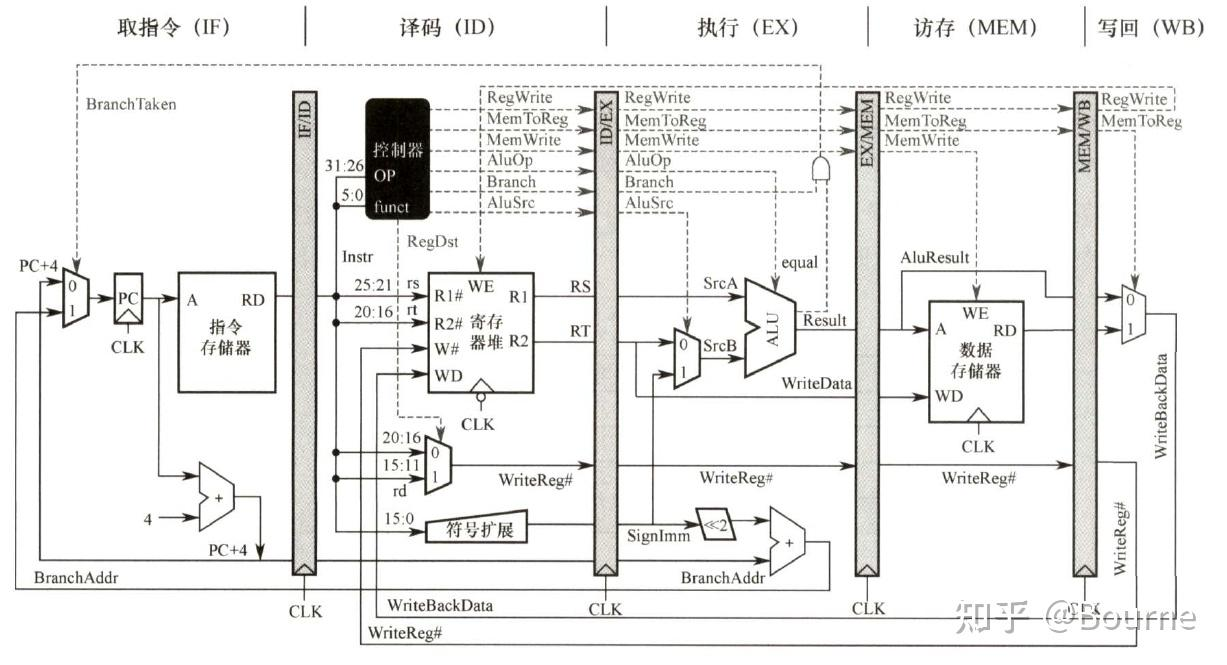
\includegraphics[width=0.8\textwidth]{106/pipeline.jpg}
  \caption{一张“臭名昭著”的流水线示意图}
\end{figure}

在实际情况下可能有三类“气泡”会让流水线停顿:
\begin{itemize}
  \item 数据冒险:当后一条指令恰好用到了前一条指令尚未写回的结果时,就会发生数据冒险,一个容易想到的解决方法是插入\textbf{气泡}(stall),让流水线停顿一段时间,直到前一条指令的结果写回。另外的解决方法是\textbf{数据转发}(或\textbf{数据前递},data forwarding),直接把前一条指令的结果旁路到后一条指令的EX级,避免停顿。
  \item 控制冒险:当遇到分支判断的时候,下一条指令的地址实际上是未知的。这时候也容易想到插入气泡来等待分支结果。为了防止这种情况,现代CPU通常会采用\textbf{分支预测}(branch prediction)技术,猜测下一条指令的地址,并提前加载到流水线中。如果猜测正确,就继续执行;如果猜测错误,就丢弃错误的指令,重新加载正确的指令,这样的代价是大约10到20个时钟周期的猜测惩罚。而怎么猜则是一个技术活,常见的方法有静态预测(例如总是猜测分支不跳转)和动态预测(例如利用历史信息来预测分支行为)。
  \item 结构冒险:当多个指令同时竞争同一个硬件资源时,就会发生结构冒险。例如,如果只有一个乘法器,而两条指令都需要使用乘法器,那么就会发生结构冒险。当然插入气泡也并非不可,而通过多端口寄存器堆、分离的指令和数据缓存等方法也可以缓解结构冒险的问题。
\end{itemize}

要是再往上提升性能,一般有三种手段:超标量(superscalar)、乱序执行(OoO)和超线程(SMT)。超标量指的是每一个周期同时发射多条指令到流水线中执行;乱序执行指的是指令不必严格按照程序顺序执行,而是可以根据数据依赖关系和资源可用性来动态调整执行顺序,只要操作数就绪了这条指令就可以抢跑,最后按指令序号重新提交结果;超线程指的是在流水线里面交替塞两条线程的指令,把闲置端口也利用起来。

以上操作对我们写代码有相当的启示:尽量保持分支可预测(有规律,少跳转),减少数据依赖(多用临时变量,少用全局变量),减少资源竞争(少用全局变量,少用锁),循环体小而整齐(减少指令数,增加指令并行度)。这样就能让流水线吃得饱饱的,性能自然就上去了。例如:
\begin{lstlisting}[language=C]
  int cnt = 0;
  for(int i = 0; i < n; i++)
    if (a[i] > 128)
      ++cnt
\end{lstlisting}
这个实践是不好的,因为数组模式随机,分支不可预测,数据依赖严重。改成下面这样就好多了:
\begin{lstlisting}[language=C]
  int cnt = 0;
  for(int i = 0; i < n; i++) {
    int flag = (a[i] > 128);
    cnt += flag;
  }
\end{lstlisting}
这样就消除了分支,数据依赖也减轻了许多,编译器大概会把上述内容编译成\texttt{setgt}和\texttt{add}指令,流水线就能更好地并行执行。

\begin{tip}
  当然,根据“不优化”原则我们知道,实际操作中未必需要严格这么写,或者说仅在以下情况差异显著:
\begin{itemize}
  \item 数据量巨大,例如n达到百万级别以上;
  \item 数据内容相当随机地分布,例如a[i]的值均匀分布在0到255之间;
  \item 编译器没有做激进优化,例如开的\texttt{-O0}或者\texttt{-O1};
  \item CPU是现代超标量、流水线深度相当大的CPU。
\end{itemize}
反之,当数据量小、大多数数据大于128(分支预测器能学习并预测)、编译器激进优化(“吸氧”甚至“吸臭氧”)、使用SIMD指令等技术时,差异就不明显了。

如希望验证我的上述说法,可以利用\texttt{perf}等工具进行性能分析,重点观察\texttt{branch-misses}、\texttt{instructions}、\texttt{cycles}等指标,\texttt{-O2}和\texttt{-O0}的差异也可以对比一下。
\end{tip}

\subsection{现代CPU的架构}

旧时代的CPU一般走的是单核高频路线,这也是非常容易想到的提升性能的方式:把一个核的频率提升到极限,然后让这个核尽可能地快地执行指令。这样做的好处是简单易行,缺点是功耗和发热量都非常高,且单核性能提升空间相当有限。这个路线撞墙的例子就是Intel的NetBurst架构(奔腾4),频率最高能达到3.8GHz,但是单核性能并没有显著提升,反而因为发热量过大而被迫降频。

于是,现代CPU性能渐渐地走向了多核化、并行化的路,性能不仅靠GHz撑着,并行度和专用加速也成为了重要的指标。当下主流芯片把多种计算单元拼成SoC,一般还有大小核之分(big.LITTLE架构),大核负责高性能计算,小核负责低功耗计算,二者协同工作以提升整体性能和能效比。

\begin{enumerate}
\item 性能核(P-core):乱序、宽发射、高频率,跑串行关键路径;
\item 能效核(E-core):顺序或窄发射,面积小、功耗低,跑后台线程;
\item 矢量/矩阵单元——SSE/AVX/AVX-512、SVE、AMX,一条指令打 512 bit–2048 bit 的 SIMD,做 dense math;
\item 集成 GPU Or NPU:上千线程级的 SIMT,负责图形与 AI 推理;
\item 片上系统:DDR/LPDDR 控制器、PCIe 5.0、CXL、缓存一致性总线(Ring/Mesh),把 CPU、GPU、加速器、内存、外设粘在一起。
\end{enumerate}

而缓存也从上文所述的经典缓存升级为支持网状多切片、非包容/非排他性、智能预取等特性的现代缓存系统,以适应多核、多线程、高并发的计算需求:

\begin{itemize}
\item 每个 P-core 独享 48 KB L1-I + 32 KB L1-D + 1–2 MB L2;
\item 多核通过 Mesh 节点共享 24–96 MB L3,切片数等于核数,降低热点;
\item 目录式(Directory)或总线嗅探(MESIF)协议保证多核一致性,跨核延迟 30–60 ns。
\end{itemize}

而对于我们开头的“超大矩阵乘法”这种还吃内存带宽的计算任务,现代CPU也有不少提升手段:

\begin{itemize}
\item AVX-512 / AMX:单指令可算 $16\times 64$ 矩阵块,理论算力提升4到8倍;
\item 高带宽内存:笔记本 LPDDR5X 已做到 120 GB/s,服务器 HBM3 突破 1 TB/s;
\item 缓存阻塞(cache blocking):把超大矩阵切成 L2 能装下的子块(如 $256 \times 256$),再在内层用 SIMD 展开,就能把 100 ns 的内存访问变成 5 ns 的 L2 命中,轻松获得10倍数级提速。
\end{itemize}

所以说,现代的CPU并不是单核跑分的时代,而是多核、矢量、缓存墙协同作战。写程序的时候,只需要让计算靠近数据、并行匹配硬件宽度,就能真正的把晶体管一滴不剩地榨成有效算力。

\section{系统怎么被调用?}

有时候我们电脑死机了,或者程序崩溃了,终端报错“Segmentation Fault”(段错误)。这时候,操作系统到底做了什么?为什么会发生段错误?我们来分析一下“系统调用”就知道了。

\subsection{为什么要有这个系统调用?}

一般情况下,程序运行时仅会访问分配给自身的内存中的数据和指令。如果程序试图访问未分配的内存区域,或者试图修改只读内存区域,就会发生段错误。这是出于安全性和稳定性的考量:操作系统需要确保每个进程都只能访问自己的内存区域,不能访问其他进程的内存区域。这样可以有效防止恶意程序破坏系统的稳定性和安全性。

但是有些情况下,程序确实需要访问一些特殊的内存区域,例如访问硬件设备、操作系统内核等。为了解决这种问题,操作系统提供了系统调用(system call)来处理内存访问。

简单地说,可以把操作系统看成化学实验室管理员,管理危化品。把危化品直接扔给学生非常危险,学生必须先向管理员填表申请,管理员检查后再给学生。填的这个表就是系统调用。

\subsection{系统调用长什么样?}

以Linux为例,一个系统调用往往包括系统调用号(放在RAX)、参数(放在RDI、RSI、RDX等寄存器,包括要干什么、干多少次、怎么干)、触发指令(\texttt{syscall})和返回值(放在RAX)。当程序需要进行系统调用时,会使用\texttt{syscall}指令来触发系统调用。系统调用的种类很多,例如read、write、open、close等,每个系统调用都有一个唯一的系统调用号。

以实验室为例,上述填表就包括:编号(系统调用号)、申请的危化品(参数)(包括要什么、要多少、放哪)、申请的指令(\texttt{syscall}),以及管理员的批复(返回值)。当学生需要使用危化品时,就会向管理员提交申请,管理员检查后返回批复。

\subsection{系统调用的处理流程}

当程序触发系统调用时,CPU会将当前的执行状态保存到内核栈中,然后切换到内核态(kernel mode)。在内核态下,操作系统会根据系统调用号找到对应的系统调用处理函数,并执行相应的操作。处理完成后,操作系统会将结果返回给用户态(user mode),并恢复之前保存的执行状态。

以\texttt{printf("Hello")}为例,这个东西实际上是做了一次系统调用\texttt{write(1, buf, 5)}。现在glibc把这玩意塞进寄存器触发syscall指令,然后CPU就切换到内核态。

之后,CPU在内核态办事:检查文件描述符1是否可写,发现可以写,就把Hello这5个字节写入到文件描述符1对应的设备(通常是终端)。

写完后,CPU会将结果(成功写入的字节数,在这里是5)放回RAX寄存器,然后切换回用户态。然后代码就会继续执行了。

\subsection{系统调用的代价与实践尝试}

系统调用虽然显著提升了系统的安全性,但是也带来了巨大的性能损失。因为每次系统调用都需要切换到内核态,这个过程需要保存和恢复CPU的状态,涉及到上下文切换(context switch),会消耗大量的时间,比普通函数调用慢不少——这还是现代CPU的优化结果。因此,系统调用的次数越少,程序的性能就越好。

在代码实践中,我们最简单的优化方式就是尽可能减少系统调用的次数,例如使用缓冲IO或批量读写等。

\begin{thinking}
  \begin{enumerate}
    \item 验证:浮点误差能累积到金融级别不可接受。试着使用不同的方法累加(不是乘法)1亿个0.01:\texttt{long double}、\texttt{double}、\texttt{float}、Kahan求和、\texttt{libmpdec}高精度库等,看看结果有什么差异。同时,使用\texttt{perf stat}等工具,看看不同方法的性能差异,量化误差和性能的权衡。最终,试着用文中提到的\texttt{int}方法来实现货币运算,看看结果和性能如何。
    \item 可执行文件究竟长什么样?GCC编译出的\texttt{*.o}和ELF文件究竟有什么差异?试着把这两个文件用十六进制编辑器打开,看看里面都有什么内容;标出ELF文件中的\texttt{e\_entry}、\texttt{program header}、\texttt{section header}等字段,并解释它们的作用。
    \item 优化究竟是怎么暴露未定义行为的?试着故意写一段有整数溢出的看似无害的UB代码,然后使用GCC编译器在不同的优化等级下编译,看看汇编码有什么差异(提示:用\texttt{diff}命令比较)。接着,试着打开UBSan运行程序,看看会发生什么。
    \item 虚拟内存真的是免费午餐吗?试着验证一下,当物理内存不足时,操作系统会将哪些页面换出到磁盘交换区?试着写一个程序,分配大量内存(例如\texttt{malloc 10GB})但不访问,观察VmSize和VmRSS的变化;然后,访问这些内存,观察VmSize和VmRSS的变化、记录SIGBUS或者真实缺页的次数,从而理解什么是overcommit(过度承诺)和OOM Killer,以及“用到才给”的含义。
    \item LRU真的永远是最优的吗?试着写一个程序,访问一个大数组(例如100MB),但是访问顺序是随机的,观察缓存命中率和程序运行时间。然后,试着改变访问顺序,例如按行访问、按列访问、斐波那契访问等,观察缓存命中率和程序运行时间的变化,从而理解局部性原理。另一方面,你能写一个程序,使得FIFO比LRU更优吗?
    \item 一条syscall指令事实上产生了多大的性能开销?试着写一个程序,频繁调用一个简单的系统调用(例如\texttt{getpid()}),然后使用\texttt{bpftrace}或者\texttt{perf}等工具,测量系统调用的延迟和CPU周期数,从而量化系统调用的开销。然后,试着将多个系统调用合并为一个系统调用(例如\texttt{io\_uring}),观察性能的提升,从而理解减少系统调用次数的重要性。
  \end{enumerate}
\end{thinking}


\part{走向开发}
\chapter{C++高速入门}

本章会快速带领大家过一遍C++的基本语法和常用特性,除了用作预习材料以外,还可以在期末考试复习的时候来快速回顾其基本语法与常用的高级特性。

这里直接从C++开始讲起,因为C++是C的超集,C的语法在C++中完全可以使用。

由于C++的语法和特性极多、语法也较为复杂,因此本章节可能会显得有些长、节奏也非常快。

让我们开始吧:

\section{C++的基本语法}

第一次写C++的时候,我们只需要了解一些最基本的语法和特性。记住以下三件事:

\textbf{程序有入口;先存再算;算完告诉外面。}剩下的内容,都跟我们说话一样,只不过是用C++的语法来表达,而且我们说话的句号在C++中是分号。

一个简单的C++程序如下:
\begin{lstlisting}[language=C++]
#include <iostream>

int main() {
    int age = 18;
    std::cout << "I am " << age;
    return 0;
}
\end{lstlisting}
逐行拆解之:
\begin{itemize}
  \item \texttt{\#include <iostream>}:告诉编译器,我要用输入输出工具。
  \item \texttt{int main()}:程序的入口函数,告诉电脑程序从这里开始执行。\texttt{int}表示这个函数返回一个整数值。
  \item \texttt{int age = 18;}:跟电脑说,我要在内存找个地方放个整数,这个地方叫age,放个18进去。
  \item \texttt{std::cout << "I am " << age; }:把东西一股脑全送到屏幕上。
  \item \texttt{return 0;}:返回0,告诉操作系统:一切OK。除非你知道你在做什么,否则这里不要改成其他数字。
\end{itemize}

以上就是骨架。接下来该往骨架里面填肉了。

\subsection{头文件、源文件}

\textbf{头文件}是一些预先写好的代码的集合。通过包含头文件,我们可以使用这些预先写好的代码,而不需要重新编写它们。头文件的扩展名通常是\texttt{.h}或\texttt{.hpp}。引入头文件只需要在文件的开头使用\texttt{\#include}指令即可。

头文件有两种类型:标准库头文件和自定义头文件。标准库头文件是C++标准库提供的头文件,通常使用尖括号括起来,例如\texttt{<iostream>}、\texttt{<vector>}等,这样会先在系统路径中查找,再去当前路径中查找;自定义头文件是用户自己编写的头文件,通常使用双引号括起来,例如\texttt{"myheader.h"},这样会先在当前路径中查找,再去系统路径中查找。

与“头文件”相对应的是\textbf{源文件},它们通常包含程序的主要逻辑和实现代码。源文件的扩展名通常是\texttt{.cpp}、\texttt{.cxx}或\texttt{.cc}。源文件可以包含头文件,并且可以定义函数、类和变量等。

\begin{lstlisting}[language=C++]
// 这是一个源文件
#include <iostream>  // 引入标准库头文件
#include "myheader.h"  // 引入自定义头文件

int main() {
    // 使用头文件中的代码
    return 0;
}
\end{lstlisting}

\begin{warning}
    严格禁止使用所谓的“万能头文件”\texttt{\# include <bits/stdc++.h>},\textbf{尤其是在工程中!}该头文件有三个严重的问题:
    \begin{itemize}
        \item 该头文件不是C++标准的与部分,而是GCC编译器提供的一个非标准头文件。使用该头文件会导致代码在不同编译器下表现不同,严重地影响代码的可移植性。
        \item 该头文件会引入整个标准库,从而显著地降低代码的可维护性,具体表现为:
        \begin{itemize}
            \item 显著地增加编译时间,尤其是在大型项目中。
            \item 引入大量实际上并不需要的库,严重地增加了命名冲突的风险。
            \item 引入大量宏定义,可能会导致意想不到的行为。
        \end{itemize}
    \end{itemize}
    综上所述,严格禁止使用该头文件!多背几个常用的头文件名称并不难,且对代码质量有显著提升。
\end{warning}

\subsection{命名空间}

我们知道,一个软件还是程序,可能由很多人来完成。为了方便,每一个人都有可能定义自己的东西,例如功能(函数)、数据(变量)等。那么,如果两个人给自己不同的东西起了同样的名字怎么办?这时,电脑就无法区分它们了。

一个简单的方法是加强沟通,减少重名的可能性。但是,这样做并不现实。有的项目可能有数百人参与,沟通成本过高;有的项目是给下游使用的,这时又不可能沟通。这个问题非常棘手。

为了解决这个问题,C++引入了\textbf{命名空间}的概念。命名空间可以参照我们说过的虚拟环境概念来理解:每一个人都有自己的一个沙盒,在自己的沙盒里可以随便起名字,互不干扰。这样一来,即使两个人起了同样的名字,也不会冲突,因为它们属于不同的命名空间。
\begin{lstlisting}[language=C++]
    namespace Alice {
        int value = 42; // 数据(变量)
        void show() {   // 功能(方法)
            std::cout << "Alice's value: " << value << std::endl;
        }
    }
    namespace Bob {
        int value = 100; // 数据(变量)
        void show() {    // 功能(方法)
            std::cout << "Bob's value: " << value << std::endl;
        }
    }
\end{lstlisting}
这样,两者并不冲突。

但是新的问题又来了:有时候,别人在他们的命名空间里写了一些东西,而这些东西又是我们想要的。为了方便起见,肯定不能写第二遍。那么,我们该怎么办呢?可以这样写:
\begin{lstlisting}[language=C++]
    Alice::show(); // 调用Alice命名空间中的show函数
    Bob::show();   // 调用Bob命名空间中的show函数   
\end{lstlisting}
于是困扰我们的重名问题就彻底解决了。

为了帮助我们更好的开发,C++提供了一些东西减少我们的重复劳动。这些东西被C++放在了“标准”命名空间中,也就是\texttt{std}。诸如\texttt{cout}、\texttt{cin}、\texttt{endl}等都在这个命名空间中。因此,我们在使用这些东西的时候,必须加上\texttt{std::}前缀,例如\texttt{std::cout}、\texttt{std::cin}、\texttt{std::endl}等。

为了方便起见,可以使用\texttt{using namespace std;}来引入整个\texttt{std}命名空间,这样在这个文件以及其下游文件中,就可以直接使用标准空间中的东西,而不需要加上\texttt{std::}前缀了。但是这样做也是有风险的:这会把整个标准命名空间都引进来,容易导致重名冲突等问题。

\begin{warning}
    严格禁止在工程头文件中使用\texttt{using namespace std;}!这会污染全局的命名空间,从而导致重名冲突等问题。头文件是给别人用的,绝对不应污染别人的命名空间。如果确实想用,我们有以下手段来解决污染命名空间问题:
    
    \begin{enumerate}
        \item 每一次使用标准命名空间中的东西时,都加上\texttt{std::}前缀。
        \begin{lstlisting}
    std::cout << "Hello, World!" << std::endl;
        \end{lstlisting}
        \item 只引入需要的东西,例如:
        \begin{lstlisting}
    using std::cout;
    using std::endl;
        \end{lstlisting}
        这样就只引入了\texttt{cout}和\texttt{endl},而不会污染其他的东西。而一般人也不会去定义诸如\texttt{cout}和\texttt{endl}这样的名字,所以这样基本上可以认为是安全的。
    \end{enumerate}
\end{warning}

\begin{caution}
    在工程上,源文件也不推荐使用\texttt{using namespace std;}。但是这样做是可以容忍的,因为源文件是给自己用的,一般不至于污染命名空间,但是风险也是相当大的。对此,这需要大家自己权衡利弊了。如果项目周期非常短(例如做题),那么这么做没有毛病。但是如果是写工程这种长周期开发,则推荐老老实实用上面提到的两种方法来避免污染命名空间。
\end{caution}

\begin{note}
    为了简便,本书中大部分代码都使用了\texttt{using namespace std;},但是请大家务必牢记上述警告和注意事项。
\end{note}

\subsection{基本变量及其运算}

变量用来存储数据,可以变化;声明格式是\textbf{“先写类型,再写名字”}。

常见的变量类型有:
\begin{itemize}
  \item \texttt{int}:整数类型,通常是64位(二进制位数,在古老的32位机器上表现为32位)。
  \item \texttt{double}:双精度浮点数,通常是64位。
  \item \texttt{char}:字符类型,通常是8位整数,表示一个字符。也可以用于表示整数。
  \item \texttt{bool}:布尔类型,表示真或假。
  \item \texttt{string}:字符串类型,表示一串字符。
\end{itemize}

对于变量的运算就跟数学差不多,比方说
\begin{lstlisting}[language=C++]
    int a = 10;
    int b = 20;
    int c = a + b;
    c = a * 2;
    c += 5;
\end{lstlisting}
\texttt{int c = a + b}的意思是“我要创建一个变量c,把a+b的结果放进去”。可以看到,从这一行以后再提到c,就不需要再写\texttt{int}了,因为电脑已经知道c是个什么东西了。

下一行\texttt{c = a * 2}的意思是“我要把a乘以2的结果放到c里面,c以前不管是什么我都不要了”,而再下一行\texttt{c += 5}的意思是“我要把c加上5”。在上述代码中,我们发现变量c的值会随着每一行代码的执行而变化,例如第三行代码执行后,c的值变成了30;第四行代码执行后,c的值变成了20;第五行代码执行后,c的值变成了25。所以说c是一个变量。

变量的值也可以在声明时不确定(初始化),例如\texttt{int a;}这样也是可以的。如果在声明的时候不初始化局部变量的值,那么这个变量的初始值将会是一个\textbf{未定义行为},这个值取决于内存中该位置之前存储的内容。我们不能依赖于这个,因此最好在声明变量的时候就给它赋初始值,例如\texttt{int a = 0;}。对于全局变量,如果不初始化,编译器会自动将其0初始化。

让我们看看常见的运算符:
\begin{itemize}
  \item 四则运算:\texttt{+}(加)、\texttt{-}(减)、\texttt{*}(乘)、\texttt{/}(除)。注意,除法运算中,如果两个整数相除,结果仍然是整数,余数会被舍弃。
  \item 取模:\texttt{\%},表示取余数。例如\texttt{5 \% 2}的结果是1,因为5除以2的余数是1。
  \item 自增和自减:\texttt{++}(自增)和\texttt{--}(自减)。例如,\texttt{a++}表示将a的值加1,\texttt{b--}表示将b的值减1。
\end{itemize}
不要过分纠结\texttt{i++}和\texttt{++i}的区别,初学者完全可以认为这两个和\texttt{i += 1}没有区别。

\begin{caution}
  尽量单独使用\texttt{++}和\texttt{--},不要把它们和其他运算混在一起使用,更不要在同一个表达式中对同一个变量使用多次\texttt{++}或\texttt{--}。例如,\texttt{a = b++}虽然不推荐但还勉强可以,但是\texttt{a = b++ + b++}和\texttt{i = i++}都是未定义行为。一个饱受诟病的题目“\texttt{i = 3, i++ + i++ = ?}”答:这个题目是错误的,至少是不良定义的。不同的编译器对上述代码的处理方式不同。

  笔者个人从工程的眼光上看来,非常不建议弄出\texttt{a = b++}这类的代码,尽管这类代码在竞赛中会让很多OIer感到Tricky,但是在工程中会让人无比恼火。如果想先用b的值再加1,可以写成\texttt{a = b; b++;};如果想先加1再用b的值,可以写成\texttt{b++; a = b;}。上述写法一般只有非常约定俗成的场合才会使用,例如\texttt{while(T--)}或者\texttt{stk[++top]=x}——不过即使是我,也更习惯于写成\lstinline[language=C++]|for(;T>0;T--)| 和 \lstinline[language=C++]|stack<int> stk; stk.push(x);|。
\end{caution}

是不是非常简单?

\subsection{注释}

注释是代码中的说明文字。它们会被编译器忽略,因此注释完全是给编写者和阅读者看的。

在C++中,注释有两种方法来写:
\begin{itemize}
  \item 单行注释:使用\texttt{//},例如\texttt{// 这是一个单行注释}。注释符号后面的内容会被编译器忽略,直到行尾为止。
  \item 多行注释:使用\texttt{/* ... */},例如\texttt{/* 这是一个多行注释 */}。两个注释符号之间的内容会被编译器忽略,可以跨越多行。
\end{itemize}

在阻止部分代码执行的时候,我们一般不习惯于直接删除这些代码,而是使用注释。这样做的好处是可以留痕,便于以后的恢复(解注释);这就是程序员们常说的“注释掉”代码。在VS Code等编辑器中,常用的一键注释是\texttt{Ctrl + /},它会自动将光标所在的一行或多行代码注释掉。

\subsection{常变量、常量}
常变量(也叫不可变变量、只读变量、运行时常量)、常量(也叫编译期常量)往往笼统地称为常量。它们一旦确定就不会\textbf{在程序运行时}改变,任何试图对它们进行运行时更改的操作都会使得编译不通过。常量的值应当在声明时确定,可以通过赋值或者计算得到。它们的名字通常使用大写字母来表示,以便于和变量区分。

声明常变量的方法和声明变量差不多,但是要在最前面加上\texttt{const}关键字,如:
\begin{lstlisting}[language=C++]
const int MAX_VALUE = 100;
const int P = a + b; // 这里的a和b可以是变量
// P = 10 // 这行代码编译不通过,因此要注释掉
\end{lstlisting}
以上代码的意思是:我要创建一个常量MAX\_VALUE,它的值是100。

如果常变量的值\textbf{必须在编译时}确定,可以使用常量。常量的值在编译的时候值就确定了,不过因此也需要在定义中就写明它的值。常量的声明方法和常变量类似,只是把\texttt{const}换成\texttt{constexpr}。

常量也可以通过计算得到,计算在编译时进行,可以节省程序运行时间,但是要求用于计算的东西也必须是常量、字面值(直接写出来的值)、constexpr函数或者立即函数\footnote{立即函数指的是声明为\texttt{consteval}的函数,在\texttt{C++20}中被引入,这样的函数\textbf{只能在编译时期调用}}。下文是常量的几个例子。

\begin{lstlisting}[language=C++]
constexpr double E = 2.71828;
constexpr double PI = 3.14159;
constexpr double EPI = E * PI;
\end{lstlisting}

在现代\texttt{C++}中,\texttt{const}常变量不依靠运行时初始化来确定其值(例如\lstinline[language=c++]|const int b = 1;|),其表现就和\texttt{constexpr}常量一样了。因此,在大多数时候,我们也可以把\texttt{const}常变量当作\texttt{constexpr}常量来使用。但如希望严谨表达意图,仍建议使用\texttt{constexpr}来声明常量。

\begin{tip}
还是不懂?可以通过以下例子理解一下变量、运行时常量、编译期常量的区别:
\begin{lstlisting}[language=C++]
    int sqr(int x) { return x * x; } // 普通函数
    const int sqr_c(const int x) { return x * x; } // const函数
    constexpr int sqr_ce(const int x) { return x * x; } // constexpr函数
    consteval int sqr_cv(const int x) { return x * x; } // consteval函数
\end{lstlisting}

那么对于以下声明,编译器的表现如下表所示。其中,编译失败的情形用红色标出;用\texttt{const}声明的运行时常量表现为编译期常量的特殊情形则使用蓝色标出。
\begin{small}            % 整体字号
\begin{longtable}[c]{l|ll}
  \caption{变量/常量声明与编译器表现}
  \label{tab:long}\\
  \toprule
  声明 & 编译器表现 & 理由 \\
  \midrule
  \endfirsthead          % 首页表头

  \multicolumn{3}{c}{\footnotesize 续表~\ref{tab:long}}\\[.5ex]
  \toprule
  声明 & 编译器表现 & 理由 \\
  \midrule
  \endhead               % 后续页表头

  \midrule
  \multicolumn{3}{r}{\footnotesize 接下页}
  \endfoot               % 每页底部(除末页)

  \bottomrule
  \endlastfoot           % 末页底部

  \texttt{int a0 = 5;} & 变量 & 显然 \\
  \rowcolor{blue!15}\texttt{const int a1 = 5;} & 编译期常量 & 不依赖运行时初始化 \\
  \texttt{constexpr int a2 = 5;} & 编译期常量 & 字面值 \\
  \texttt{const int a3 = a0;} & 运行时常量 & 依赖运行时值\texttt{a0} \\
  \rowcolor{red!15}\texttt{constexpr int a4 = a0;} & 编译失败 & 严格编译期常量不能用运行时值初始化 \\
  \texttt{int a5 = sqr(1);} & 变量 & 显然 \\
  \texttt{const int a6 = sqr(1);} & 运行时常量 & 依赖运行时函数 \\
  \rowcolor{red!15}\texttt{constexpr int a7 = sqr(1);} & 编译失败 & 严格编译期常量不能用运行时函数初始化 \\
  \texttt{int a8 = sqr\_c(1);} & 变量 & 显然 \\
  \texttt{const int a8 = sqr\_c(1);} & 运行时常量 & 依赖运行时函数 \\
  \rowcolor{red!15}\texttt{constexpr int a9 = sqr\_c(1);} & 编译失败 & 严格编译期常量不能用运行时函数初始化 \\
  \texttt{int a10 = sqr\_ce(1);} & 变量 & 显然 \\
  \rowcolor{blue!15}\texttt{const int a11 = sqr\_ce(1);} & 编译期常量 & \texttt{constexpr}函数接受常量则在编译期初始化 \\
  \texttt{const int a12 = sqr\_ce(a0);} & 运行时常量 & 依赖运行时值\texttt{a0} \\
  \texttt{constexpr int a13 = sqr\_ce(1);} & 编译期常量 & 显然 \\
  \rowcolor{red!15}\texttt{constexpr int a14 = sqr\_ce(a0);} & 编译失败 & 严格编译期常量不能用运行时值初始化 \\
  \rowcolor{red!15}\texttt{int a15 = sqr\_cv(1);} & 编译失败 & 立即函数不可以在运行时调用 \\
  \rowcolor{blue!15}\texttt{const int a16 = sqr\_cv(1);} & 编译时常量 & 显然 \\
  \rowcolor{red!15}\texttt{const int a17 = sqr\_cv(a0);} & 编译失败 & 立即函数不可以在运行时调用 \\
  \texttt{constexpr int a18 = sqr\_cv(1);} & 编译时常量 & 显然 \\
  \rowcolor{red!15}\texttt{constexpr int a19 = sqr\_cv(a0);} & 编译失败 & 立即函数不可以在运行时调用 \\
\end{longtable}
\end{small}
\end{tip}

\subsection{判断和循环}
有时候,代码需要根据不同的条件或不同的输入来执行不同的操作;有时候,一段代码需要执行很多次,但是并不知道具体要执行多少次。C++提供了条件语句和循环语句来实现这些功能。

\subsubsection{条件表达式}
条件表达式是一个布尔表达式,它的值要么是true(真),要么是false(假)。在C++中,条件表达式通常用于控制程序的执行流程。一般情况下,认为false等价于0,true等价于1;而且在需要布尔值的地方,非零值会被视为true,零值会被视为false。

常见的一些条件表达式包括:
\begin{itemize}
  \item \texttt{==}:等于运算符。
  \item \texttt{!=}:不等于运算符。
  \item \texttt{<}:小于运算符。
  \item \texttt{>}:大于运算符。
  \item \texttt{<=}:小于等于运算符。
  \item \texttt{>=}:大于等于运算符。
  \item \texttt{\&\&}:逻辑与运算符。如果前后两个条件都为真,则结果为真;有一个是假的话,结果为假。
  \item \texttt{||}:逻辑或运算符。如果前后两个条件至少有一个为真,则结果为真;如果两个都为假,结果为假。
  \item \texttt{!}:逻辑非运算符。如果后面跟着的条件是真的,那么结果为假;反之为假。
\end{itemize}

\begin{tip}
    在C++中,不能使用类似\texttt{1 <= x <= 2}这样的连续记号来表示区间。正确的写法是\texttt{(1 <= x) \&\& (x <= 2)},即把每个比较都单独写出来,然后用逻辑与运算符连接起来。
\end{tip}

在C++中,与或非运算符是有一定的运算顺序的。一般情况下,逻辑非运算符的优先级最高,其次是逻辑与运算符,最后是逻辑或运算符。不过笔者非常不建议同学们背诵这个顺序;实际在工程上不仅不建议大量嵌套使用这些运算符,而且遇事不决可以加括号——括号可比记运算顺序靠谱得多了!

\subsubsection{条件语句}

最常见的条件语句是\texttt{if}语句。它的基本格式如下:
\begin{lstlisting}[language=C++]
if (条件) {
    // 条件为真时执行的代码
}
else if (另一个条件) {
    // 另一个条件为真时执行的代码
}
else {
    // 以上条件全部为假时执行的代码
}
\end{lstlisting}
以上代码可以有很多个\texttt{else if}分支,也可以没有\texttt{else}分支。意思是:我执行到if这一行的时候,检查后面的条件。如果条件为真,那么执行第一个大括号内的代码,剩下的全都不执行;如果条件为假,那么检查下一个\texttt{else if}的条件,如果为真就执行它的大括号内的代码,剩下的全不执行;如果所有的条件都为假,那么执行\texttt{else}大括号内的代码。

例子:
\begin{lstlisting}[language=C++]
if (age < 18) {
    cout << "未成年";
}
else if (age < 60) {
    cout << "成年人";
}
else {
    cout << "老年人";
}
\end{lstlisting}
一目了然,不言而喻。这个age变量可以是前面提到的许多类型。

\subsubsection{三元表达式}

三元表达式也是一种条件表达式,只不过它可以在一行代码中完成条件判断和结果返回,因此显得更简洁。它通常用于简单的条件判断和赋值操作。它的基本格式如下:
\begin{lstlisting}[language=C++]
条件 ? 真值 : 假值
\end{lstlisting}
以上代码的意思是:如果条件为真,整个表达式的值和真值一样;否则,整个表达式的值和假值一样。它非常适合简单的条件判断和赋值操作,但是我们不建议在复杂的条件判断中使用它或者者嵌套使用它,这样会大大降低代码的可读性。

比方说,我们可以用它来判断一个数是奇数还是偶数:
\begin{lstlisting}[language=C++]
int n = 5;
string result = (n % 2 == 0) ? "偶数" : "奇数";
\end{lstlisting}
以上代码的意思是:如果n是偶数,就把字符串“偶数”赋值给result;否则把字符串“奇数”赋值给result。

如果使用if语句来实现同样的功能,可以写成:
\begin{lstlisting}[language=C++]
int n = 5;
string result;
if (n % 2 == 0) {
    result = "偶数";
} else {
    result = "奇数";
}
\end{lstlisting}

\subsubsection{切换语句}
有时候,我们需要根据一个变量的值来执行不同的操作。C++提供了\texttt{switch}语句来实现这个功能。它的基本格式如下:
\begin{lstlisting}[language=C++]
switch (变量) {
    case 值1:
        // 当变量等于值1时执行的代码
        break;
    case 值2:
        // 当变量等于值2时执行的代码
        break;
    default:
        // 当变量不等于任何case的值时执行的代码
}
\end{lstlisting}
以上代码的意思是:检查变量的值,如果等于值1,就执行第一个大括号内的代码;如果等于值2,就执行第二个大括号内的代码;如果都不等于,就执行\texttt{default}大括号内的代码。可以有任意多个\texttt{case}分支,也可以没有\texttt{default}分支。

注意,\texttt{break}语句用于跳出\texttt{switch},这个是必须的。

例子:
\begin{lstlisting}[language=C++]
switch (day) {
    case 1:
        cout << "星期一";
        break;
    case 2:
        cout << "星期二";
        break;
    case 3:
        cout << "星期三";
        break;
    // ......其他的,基本一个写法
}
\end{lstlisting}
这也一目了然不言而喻了。

\subsubsection{for循环语句}

for循环是灵活度极高的循环语句。它的基本格式如下:
\begin{lstlisting}[language=C++]
for (初始化; 条件; 更新) {
    // 循环体
}
\end{lstlisting}
以上代码的意思是:先执行初始化语句,然后检查条件是否为真。如果为真,就执行循环体内的代码,然后执行更新语句。接着再检查条件,如果为真就继续执行循环体,否则跳出循环。比方说,我们需要打印1到10的数字,可以这样写:
\begin{lstlisting}[language=C++]
for (int i = 1; i <= 10; i++) {
    cout << i << " ";
}
\end{lstlisting}
这段代码的意思是:先初始化一个变量i为1,然后检查i是否小于等于10。如果是,就打印i的值,然后将i加1。接着再检查i是否小于等于10,如果是就继续打印,否则跳出循环。

这个\texttt{int i = 1}可以在其他地方声明过,那么这里就遵从“先声明后使用”的原则,不需要再写int了。

\subsubsection{while和do-while循环语句}
while循环是另一种常见的循环语句。它的基本格式如下:
\begin{lstlisting}[language=C++]
while (条件) {
    // 循环体
}
\end{lstlisting}
以上代码的意思是:先检查条件是否为真。如果为真,就执行循环体内的代码,然后再次检查条件。如果条件仍然为真,就继续执行循环体,否则跳出循环。比方说,我们需要打印1到10的数字,可以这样写:
\begin{lstlisting}[language=C++]
int i = 1;
while (i <= 10) {
    cout << i << " ";
    i++;
}
\end{lstlisting}
以上内容与for循环的例子是等价的。

do-while循环与while循环类似,但它会先执行一次循环体,然后再检查条件。它的基本格式如下:
\begin{lstlisting}[language=C++]
do {
    // 循环体
} while (条件);
\end{lstlisting}
这样可以保证循环体至少执行一次。比方说,我们需要打印1到10的数字,可以这样写:
\begin{lstlisting}[language=C++]
int i = 1;
do {
    cout << i << " ";
    i++;
} while (i <= 10);
\end{lstlisting}

\subsubsection{break和continue语句}

有时候,我们需要在循环中提前跳出循环或者跳过当前的迭代。C++提供了\texttt{break}和\texttt{continue}语句来实现这些功能,它们也叫做循环控制语句。

\texttt{break}语句用于跳出循环,通常用于满足某个条件时立即结束循环。例如:
\begin{lstlisting}[language=C++]
for (int i = 1; i <= 10; i++) {
    if (i == 5) {
        break;  // 当i等于5时跳出循环
    }
    cout << i << " ";
}
\end{lstlisting}
上述代码如果不写break一句,那么会输出1到10;如果写了break一句,那么会输出1到4。

而continue语句只用于跳过当前循环的剩余语句,继续下一次迭代。例如:
\begin{lstlisting}[language=C++]
for (int i = 1; i <= 10; i++) {
    if (i == 5) {
        continue;  // 当i等于5时跳过当前迭代
    }
    cout << i << " ";
}
\end{lstlisting}
上述代码的输出应该是1 2 3 4 6 7 8 9 10。因为当i等于5时,continue语句会跳过当前迭代的输出语句。

\subsection{输入输出}

在C++中,我们建议使用更安全的输入输出流\texttt{cin}和\texttt{cout}来进行输入输出操作。它们分别用于从标准输入(通常是键盘)读取数据和向标准输出(通常是屏幕)打印数据。

\texttt{cin}和\texttt{cout}的基本用法如下:
\begin{lstlisting}[language=C++]
#include <iostream>
using namespace std;
int main() {
    int age;
    cout << "请输入你的年龄:";  // 输出提示信息
    cin >> age;  // 从标准输入读取数据
    cout << "你输入的年龄是:" << age << endl;  // 输出读取到的数据
    return 0;
}
\end{lstlisting}
以上代码的意思是:先输出提示信息“请输入你的年龄:”,然后从标准输入读取一个整数值并存储到变量age中。接着输出“你输入的年龄是:”以及读取到的年龄值。

C风格的输入输出分别是\texttt{printf}和\texttt{scanf},它们的用法如下:
\begin{lstlisting}[language=C++]
#include <cstdio>
// 也可以写成 #include <stdio.h>,但不推荐
using namespace std;
int main() {
    int age;
    printf("请输入你的年龄:");  // 输出提示信息
    scanf("%d", &age);  // 从标准输入读取数据
    printf("你输入的年龄是:%d\n", age);  // 输出读取到的数据
    return 0;
}
\end{lstlisting}
以上代码中,\texttt{\%d}的意思是“这里要输出一个整数”,而\texttt{\&age}的意思是“把age的地址传给scanf”。前者叫做“格式化输出”,后者叫做“地址传递”。这两个函数也是有自己的返回值的:\texttt{printf}返回成功输出的字符数,而\texttt{scanf}返回成功读取的项数。

\texttt{printf}和\texttt{scanf}的速度更快,因为不需要流操作;但是它们存在一些安全隐患,例如格式化字符串攻击和缓冲区溢出等问题。现代C编程中,微软推荐使用\texttt{scanf\_s}和\texttt{printf\_s}来代替\texttt{scanf}和\texttt{printf},它们允许一个额外的参数来指定缓冲区的大小,从而避免缓冲区溢出的问题。但是,gcc和clang均不支持这两个函数。

不过,虽然在做题的时候确实可以使用\texttt{scanf}和\texttt{printf}来压榨时间,但是我们仍然建议在C++工程上使用更安全的\texttt{cin}和\texttt{cout}。

另外,我们在写代码的时候{\color{red}\textbf{一定不要一句C一句C++,或者说不要一句printf一句cout(反过来也不行)}},这样会导致缓冲区冲突,从而引发一些莫名其妙的问题。要么全用C的输入输出,要么全用C++的输入输出。

\begin{note}
  实际上,\texttt{cin}和\texttt{cout}和\texttt{printf}和\texttt{scanf}区别巨大。后者是一个函数,而前者是一个“流对象”(可以理解为一个“东西”而不是一个“手段”)。它们是C++标准库中的流对象,真正负责输入输出的实际上是\texttt{<istream>}头文件中的\texttt{istream::read}和\texttt{<ostream>}头文件中的\texttt{ostream::write}方法,它们被封装进\texttt{>>}和\texttt{<<}这两个运算符(流运算符),和我们的加减乘除等运算符一样。这两个运算符必然是返回流对象的一个引用,因此可以链式调用。特别的,当输入失败的时候,会返回流对象的一个“失败”状态,因此可以通过\texttt{cin.fail()}来判断输入是否成功,也可以通过布尔上下文转换(例如\texttt{while(cin>>n)})来判断输入是否成功。

  流运算符也不是\texttt{>>}和\texttt{<<}的原本样子。它们原本是右移和左移运算符:例如\texttt{a<<b}是对a进行左移操作,将a的二进制表示整体向左边移动b位,右边补0;右移类似(只不过对于有符号整数最高位是0补0,是1补1;无符号整数默认补0)。在\texttt{<iostream>}头文件中,这两个运算符被重载了,使得它们可以用于流对象,进而辅助执行输入输出操作;也正因此,我们需要引用上述头文件才能使用它们。不过值得庆幸的是,我们可能一辈子都不会用到它们的原本样子。

  头文件\texttt{<stdio.h>}是C的头文件,而\texttt{<cstdio>}是这个头文件在C++中的移植版本。两者内容完全一致,只不过\texttt{<cstdio>}使用了C++的命名空间(\texttt{std});但是由于C++是C的超集,因此大多数实现也允许不套命名空间直接用\texttt{printf}等。在现代风格的C++编程中,我们通常使用\texttt{<iostream>}或\texttt{<cstdio>}来进行输入输出操作,而不是使用\texttt{<stdio.h>}。
\end{note}

这些看起来都非常简单。而以上内容就是C++的全部基本语法了:是的,你已经学完了!

\subsection{小练}

\begin{example}
  角谷猜想是一个有趣的数学问题:从任意整数开始,如果他是奇数就乘以3加1,如果是偶数就除以2,如此反复循环,最终一定会得到1。目前还没有人证明这个猜想,但我们可以用C++来验证一些具体值。请编写一个C++程序,输入一个整数n,然后输出这个整数经过角谷猜想的处理后,最终得到1的过程。要求输出每一步的结果。例如,输入n=6时,输出应该是:6, 3, 10, 5, 16, 8, 4, 2, 1。
\end{example}

\begin{answer}
  一句一句地看:任意整数,奇数乘以3加1,偶数除以2。这一段代码写起来很方便。我们知道,整数的奇偶性可以通过取模来判断:如果n\%2==0,那么n是偶数;否则n是奇数。

  因此仅仅这句话,从人的自然语言到代码语言的转换就非常简单了。
\begin{lstlisting}[language=C++]
int n;
if(n % 2 == 0) {
    n /= 2; // 偶数除以2
} else {
    n = n * 3 + 1; // 奇数乘以3加1
}
\end{lstlisting}

  或者使用三元表达式:
\begin{lstlisting}[language=C++]
n = (n % 2 == 0) ? (n / 2) : (n * 3 + 1);
\end{lstlisting}

  然后是下一句话:如此反复循环。这说明我们至少需要写一个循环语句。再看下一句:最终一定会得到1。

  这样我们就明确了:我们需要写一个循环语句,跳出循环的条件是n等于1。于是我们可以写成:
\begin{lstlisting}[language=C++]
while(n != 1){
    // 处理 n 的代码
}
\end{lstlisting}

  再看下一句:输入一个整数n,输出每一步的结果。这说明我们需要一个输入语句和一个输出语句。输入语句可以用\texttt{cin},输出语句可以用\texttt{cout}。

  题目读完了,那么我们就可以把这些代码组合起来了:
\begin{lstlisting}[language=C++]
int n;
cin >> n; // 输入一个整数n
cout << n; // 输出初始值
while(n != 1) {
    if(n % 2 == 0) {
        n /= 2; // 偶数除以2
    } else {
        n = n * 3 + 1; // 奇数乘以3加1
    }
    cout << " " << n; // 输出每一步处理后的结果
}
\end{lstlisting}
  这就是基本的代码框架。下一步,我们结合一开始说的话:程序要有入口,先存再算,算完告诉外面。于是我们可以真正地完成这段代码:
\begin{lstlisting}[language=C++]
#include <iostream>
using namespace std;

int main() {
    int n;
    cin >> n; // 输入一个整数n
    cout << n; // 输出初始值
    while(n != 1) {
        if(n % 2 == 0) {
            n /= 2; // 偶数除以2
        } else {
            n = n * 3 + 1; // 奇数乘以3加1
        }
        cout << " " << n; // 输出每一步处理后的结果
    }
    return 0; // 返回0,表示程序正常结束
}
\end{lstlisting}
  这段代码就是一个完整的C++程序了。同学们可以在自己的电脑上编译运行,看看效果!
\end{answer}

\begin{exercise}
  用三元表达式来改写这个程序。
\end{exercise}

\section{C++的进阶使用}

\subsection{宏和预处理指令}

宏是一种预处理指令,它可以在编译之前对代码进行替换和扩展。宏的基本格式如下:
\begin{lstlisting}[language=C++]
#define 宏名 替换内容
\end{lstlisting}
宏在编译器对代码进行预处理的时候进行纯文本替换。宏名通常使用大写字母来表示,以便于和变量区分。替换内容可以是任意的代码片段,包括变量、表达式、语句等。宏常用于定义常量,但是用宏定义的常量没有类型,而是字面值。

我们可能会看到,诸如\texttt{\#define}、\texttt{\#include}等均以符号\texttt{\#}开头,这些都是预处理指令,有时候也叫做编译指令。预处理指令和常规代码的行为有区别:它们实际上并非代码的一部分,而是在编译器对代码进行预处理的时候进行处理的。预处理指令通常用于定义宏、包含头文件、条件编译等。常用的预处理指令还有\texttt{\#pragma}、\texttt{\#ifdef}等。活用编译指令可以让代码更灵活、更高效。

\begin{tip}
    用宏定义的常量和用\texttt{const}或\texttt{constexpr}定义的常量有一些区别。宏定义的常量没有类型,因此在使用时需要注意类型转换的问题;而\texttt{const}或\texttt{constexpr}定义的常量有类型,可以更好地进行类型检查和转换。此外,宏定义的常量在预处理阶段进行替换,因此可能会导致一些意想不到的问题,例如宏展开时的优先级问题等。而\texttt{const}或\texttt{constexpr}定义的常量在编译阶段进行处理,更加安全可靠。  
\end{tip}

\begin{warning}
    严格禁止使用所谓的“火车头”预处理指令!

    所谓的火车头预处理指令,指的是在代码的开头使用大量的\texttt{\#pragma}来指定编译器的行为。这种做法显著地导致了代码的可移植性和可维护性变差。因为不同的编译器对\texttt{\#pragma}的支持程度不同,甚至同一编译器的不同版本对某些\texttt{\#pragma}的支持也可能不同。而且你辛辛苦苦打一大堆\texttt{\#pragma},实际上优化效果还不如一个简单的\texttt{-O3}。这种完全属于歪门邪道的做法,严重违反了代码简洁和可维护的原则。
\end{warning}

\subsection{更进阶的变量类型}
C++提供了许多更进阶的变量类型和特性,可以帮助我们更好地组织代码和数据。以下是一些常见的进阶变量类型和特性:
\subsubsection{数组(C风格)}

数组是一个可以存储多个同类型数据的变量。它的基本格式如下:
\begin{lstlisting}[language=C++]
类型 数组名[大小];
\end{lstlisting}
以上代码的意思是:声明一个名为数组名的数组,它可以存储大小个同类型的数据。数组的索引从0开始。例如,我们可以声明一个整数数组来存储10个整数:
\begin{lstlisting}[language=C++]
int arr[10];
\end{lstlisting}
以上的数组arr中的元素可以通过索引来访问,例如arr[0]表示第一个元素,arr[1]表示第二个元素,以此类推,一直到arr[9]表示第十个元素。没有arr[10],访问这个会出错。我们不能像Python一样访问arr[-1],因为C++不支持负索引。

在C和C++中,数组的大小应当是一个字面值、常量或常变量,或者说C风格的数组是\textbf{无法动态扩展的}。

\begin{caution}
  变长数组(VLA)是C99标准引入的特性,允许数组的大小在运行时确定,但它在C11中被变为可选特性。C++不支持任何VLA特性。容易引起误会的是,GCC 和 Clang++ 编译器提供了包含 VLA 的GNU 扩展语法,并且默认引入这些扩展,因此,VLA (例如\texttt{int n; int a[n];})在这些编译器下可行。反之,如果关闭这些扩展(通过添加 \texttt{--pedantic-errors} 选项)或者非 GNU 兼容的编译器(如 MSVC),则 VLA 不可用。在实际操作中,我们不要去写VLA,它们可能会导致代码在不同编译器下的表现不一致。C中,我们需要使用数组但是长度不确定的时候,可以将数组开得大一些,例如题目有1000个元素,那么就开1000个元素或者稍多元素的数组;C++中,我们可以使用向量\texttt{std::vector}来代替数组,该类可以动态扩展。
\end{caution}

\subsubsection{字符串}
C++风格的字符串类型是\texttt{std::string},它可以存储一串字符。字符串的基本格式如下:
\begin{lstlisting}[language=C++]
#include <string>   // 引入字符串库
string str = "Hello, World!";
\end{lstlisting}
引用字符串库是必要的,否则编译器可能会报错;这个库还提供了一些对字符串进行操作的方法,非常方便。

字符串的本质是一个数组,存储了一串字符(C风格的字符串正是char[])。我们可以通过索引来访问字符串中的字符,例如str[0]表示第一个字符,str[1]表示第二个字符,以此类推。

字符串的长度可以通过\texttt{str.length()}方法来获取。除此以外,还有很多字符串操作方法,例如\texttt{str.substr()}(获取子串)、\texttt{str.find()}(查找子串)等。

字符串是一个复杂类,和以上提到的所有数据类型都有区别。具体为什么是“复杂类”,这涉及到C++的面向对象编程(OOP)特性。我们会在后续章节中详细介绍。

\subsubsection{结构体}
结构体是一个可以存储多个不同类型数据的变量。它的基本格式如下:
\begin{lstlisting}[language=C++]
struct 结构体名 {
    类型 成员名1;
    类型 成员名2;
    // ...
};
\end{lstlisting}
以上代码的意思是:声明一个名为结构体名的结构体,它可以存储多个不同类型的数据。结构体的成员可以是任意类型,包括基本类型、数组、字符串等。
例如,我们可以声明一个表示学生的结构体:
\begin{lstlisting}[language=C++]
struct Student {
    string name;  // 学生姓名
    int age;      // 学生年龄
    double gpa;   // 学生绩点
};

Student student1;  // 声明一个学生变量
student1.name = "Alice";  // 设置学生姓名
student1.age = 20;  // 设置学生年龄
student1.gpa = 3.5;  // 设置学生绩点
cout << "Name: " << student1.name << ", Age: "
     << student1.age << ", GPA: " << student1.gpa << endl;
\end{lstlisting}

以上内容很好地展示了怎么定义、声明、使用一个结构体。结构体的成员可以通过点(.)运算符来访问,例如\texttt{student1.name}表示学生1的姓名。

结构体可以帮助我们更好地组织数据,使得代码更易读。

\subsubsection{联合体}

联合体(union)是一个特殊的结构体,它的所有成员共享同一块内存空间。联合体的基本格式如下:
\begin{lstlisting}[language=C++]
union 联合体名 {
    类型 成员名1;
    类型 成员名2;
    // ...
};
\end{lstlisting}
以上代码的意思是:声明一个名为联合体名的联合体,它可以存储多个不同类型的数据,但它们共享同一块内存空间。联合体的成员可以是任意类型,包括基本类型、数组、字符串等。

例如,我们可以声明一个表示数据的联合体:
\begin{lstlisting}[language=C++]
union Data {
    int intValue;       // 整数值
    float floatValue; // 双精度浮点数值
};
Data data;  // 声明一个数据变量
data.intValue = 42;  // 设置整数值
cout << "Int Value: " << data.intValue << endl;
\end{lstlisting}
以上代码的意思是:声明一个名为Data的联合体,它可以存储整数值、双精度浮点数值和字符值。我们可以通过访问联合体的成员来获取数据。

当然,对于上述代码中使得data为int的值为42的情况,data中的其他成员也已经随之确定:也就是把floatValue的二进制表示设定为42的二进制表示。但是,根据Mini ICS的知识我们知道,整数和浮点数的二进制表示是不同的,因此这个浮点数是一个确定的值,但它并不是42。

\subsubsection{枚举}

枚举是一个可以存储一组命名常量的变量。

枚举有两种类型,一种是传统无作用域枚举\texttt{enum},另一种是C++11引入的有作用域枚举\texttt{enum class}(也叫强枚举)。它们的区别在于,传统无作用域枚举的常量可以直接访问,枚举名和枚举值都泄漏到所在的作用域;而有作用域枚举的常量需要通过枚举名来访问。

传统无作用域枚举的基本格式如下:
\begin{lstlisting}[language=C++]
    enum Color { RED, GREEN=5, BLUE };
\end{lstlisting}
一般情况下,枚举的底层类型由编译器自选,只要能够容纳所有的值就行了,一般是\texttt{int}。常量从0开始依次递增,例如上面的RED的值为0。也可以设定枚举的值,上文中我们将GREEN的值设定为5,那么BLUE的值就是6。调用这种枚举非常简单:
\begin{lstlisting}[language=C++]
Color color = RED; // 正统调用,color的值为0
int n = RED; // 不报错,n的值为0
Color c = 7; // 不报错,但是c的值不是RED、GREEN、BLUE中的任何一个,属于有效但未命名的值
\end{lstlisting}
可以看出,这种枚举没有类型安全性,也没有作用域隔离。

有作用域枚举的基本格式如下:
\begin{lstlisting}[language=C++]
    enum class Color : std::uint8_t { RED, GREEN=5, BLUE };
\end{lstlisting}
上述强枚举的枚举名被限定在作用域内,因此只能通过类似\texttt{Color::RED}来访问。强枚举的底层类型可以显式指定,例如上面的\texttt{std::uint8\_t}。如果不指定,默认是\texttt{int}。调用这种枚举智能使用上述的正统调用:
\begin{lstlisting}[language=C++]
Color color = Color::RED; // 正确,color的值为0
int n = Color::RED; // 报错,不能将Color类型赋值给int类型
Color c = 6; // 报错,不能将int类型赋值给Color类型
int n = static_cast<int>(Color::RED); // 正确,n的值为0
\end{lstlisting}
可以看出,这种枚举有类型安全性,也有作用域隔离。

枚举作为一个数据类型很笨,不仅没有任何方法,也不能进行运算,唯一的作用是定义一组常量,便于阅读;在\texttt{switch}语句中的使用较为多见。而剩下的很多方法,都不得不手动定义。

例如下列代码中,我们定义了一个枚举的遍历方法:
\begin{lstlisting}[language=C++]
enum class Color : std::uint8_t {
    FIRST=RED,
    RED=0,
    GREEN=1,
    BLUE=2,
    LAST=BLUE
};

for (Color c = Color::FIRST; c <= Color::LAST; c = static_cast<Color>(static_cast<int>(c) + 1)) {
    // 遍历 Color 枚举的所有值
}
\end{lstlisting}
这段代码中,我们定义了一个Color枚举,并且手动定义了FIRST和LAST两个常量,分别表示枚举的第一个值和最后一个值。

\subsection{指针}

指针可以说是奠定C和C++地位的最重要特性之一,它允许用户像汇编一样直接操作内存地址。

指针实际上也是一个变量,但是它并不是像前文所说的变量“存储数据”,而是“存储地址”。例如,我们\texttt{int a = 10},这个a确实是一片内存空间,但是我们没办法利用a访问这片内存空间的地址。指针可以做到这一点。比如说,\texttt{int* p = \&a},这个p就是一个指针,它存储了变量a的地址(\&a)。我们可以通过\texttt{*p}来访问这个地址上的数据。

如果依然云里雾里,可以试着print一下\texttt{p}和\texttt{*p}的值。我们发现,前者输出的是一串十六进制数,而后者输出的是10。

我们可以利用指针进行一些较为高级的控制。例如控制数组的访问、动态内存分配等。比方说:

\begin{lstlisting}[language=C++]
int arr[5] = {1, 2, 3, 4, 5};  // 声明一个数组
int* p = arr;  // 声明一个指针,指向数组的首元素
for (int i = 0; i < 5; i++) {
    cout << *(p + i) << " ";  // 通过指针访问数组元素
}
\end{lstlisting}

指针是一种非常强大的工具,但也需要小心使用。错误地使用指针可能会导致程序崩溃或内存泄漏,有时候也有可能会导致悬空指针的问题。悬空指针是指指向已经释放的内存空间的指针,这种指针无法访问有效的数据,可能会导致程序崩溃或产生不可预知的后果。除此之外,滥用指针还可能导致指向错误的、未初始化的地址等,这些被称为“野指针”。

\begin{tip}
  悬空指针不是空指针!空指针是指向空地址的指针,是安全的;悬空指针是指向已经释放的内存空间(现在可能已经装进去一些其他数据)的指针,是不安全的。
\end{tip}

在C++中,有一些比较高级的指针特性,例如智能指针(smart pointer)。它可以自动管理内存,避免内存泄漏和野指针等问题。常见的智能指针有\texttt{std::unique\_ptr}、\texttt{std::shared\_ptr}和\texttt{std::weak\_ptr}。这些指针都是C++标准库中的类,提供了一些方法来管理内存和引用计数等:\texttt{std::unique\_ptr}表示独占所有权的指针,不能被复制,只能被移动;\texttt{std::shared\_ptr}表示共享所有权的指针,可以被多个指针共享,使用引用计数来管理内存;\texttt{std::weak\_ptr}表示弱引用的指针,不会影响引用计数,可以用于解决循环引用的问题。

\subsection{引用}

引用是C++中的一个重要特性,它允许我们创建一个变量的别名。引用的基本格式如下:
\begin{lstlisting}[language=C++]
类型& 引用名 = 原变量名;
\end{lstlisting}
以上代码的意思是:声明一个名为引用名的引用,它是原变量名的别名。引用的作用是可以通过别名来访问原变量。例如,我们可以声明一个整数的引用:
\begin{lstlisting}[language=C++]
int a = 10;  // 声明一个整数变量
int& ref = a;  // 声明一个整数的引用
cout << "a: " << a << ", ref: " << ref << endl;
ref = 20;  // 修改引用的值
cout << "a: " << a << ", ref: " << ref << endl;
\end{lstlisting}

以上代码的意思是:声明一个名为ref的引用,它是变量a的别名。我们可以通过ref来访问a。当我们修改ref的值时,实际上也修改了a的值。

引用的本质其实也是一个指针,但是它的语法简洁得多。引用可以用于函数参数传递、返回值等场景,可以避免不必要的内存拷贝,提高程序性能。在C++中,比起指针,我们更推荐使用安全、简洁的引用。

\subsection{函数和变量的作用域}

有时候,我们需要在这个地方使用一些代码,在另外一个地方也使用同样的代码。为了避免重复编写代码,我们可以将这些代码封装成一个函数。函数是一个可以重复调用的代码块,它可以接受参数并返回结果。

函数的基本格式如下:
\begin{lstlisting}[language=C++]
返回类型 函数名(参数列表) {
    // 函数体
    return 返回值;  // 如果返回类型不是void,则需要返回一个值
}
\end{lstlisting}
以上代码的意思是:声明一个名为函数名的函数,它可以接受参数列表中的参数,并返回一个返回类型的值。函数体是函数的具体实现。

例如,我们可以声明一个计算两个整数和的函数:
\begin{lstlisting}[language=C++]
int add(int a, int b) {
    return a + b;  // 返回a和b的和
}
\end{lstlisting}
我们可以在其他函数中调用这个函数:
\begin{lstlisting}[language=C++]
int main() {
    int x = 5;
    int y = 10;
    int sum = add(x, y);  // 调用add函数
    cout << "Sum: " << sum << endl;  // 输出结果
    return 0;
}
\end{lstlisting}

函数可以有任意数量的参数,也可以没有参数。函数的返回类型可以是任意类型,包括基本类型、结构体、数组等。如果函数不需要返回值,可以将返回类型设置为\texttt{void}。

我们发现,在上述方法add中定义的变量a和b只能在函数add内部使用,不能在其他地方使用。这是因为函数的作用域是局部的。这说明,变量具有一定的可访问范围,我们把这个可访问范围叫做“作用域”。一般来说,全局变量在任何位置都可以访问,而局部变量只能在它所在的函数或代码块中访问。

\subsection{函数的递归调用}

函数可以调用自己,这种调用方式叫做递归。递归函数通常用于解决一些具有重复结构的问题,例如计算阶乘、斐波那契数列等。
递归函数的基本格式如下:
\begin{lstlisting}[language=C++]
int foo(){
    if (base_case) {
        return base_value;  // 基础情况,直接返回结果
    } else {
        return foo();  // 递归调用
    }
}
\end{lstlisting}

以上代码:在执行第一个foo的时候,会判断是不是基本情况,如果是则直接结束;如果不是,则会调用foo函数本身。这个过程会一直重复,直到满足基本情况为止。某种程度上,递归也是一种循环的形式。

需要注意的是,递归需要一个基础情况来跳出递归,否则则会产生无限递归错误。例如,我们都知道计算阶乘可以使用$n!=n\times(n-1)!$,但是只有这一个公式是不够的,不停地递归下去没有尽头。这时候,我们需要一个基础情况来结束递归:$0!=1$。因此,我们可以写出递归公式:$factorial(n) = n \times factorial(n-1)$,其中$factorial(0) = 1$。然后,我们就可以用程序语言来描述这个数学语言:
\begin{lstlisting}[language=C++]
int factorial(int n) {
    if (n == 0) {
        return 1;  // 基础情况
    } else {
        return n * factorial(n - 1);  // 递归调用
    }
}
\end{lstlisting}

\subsection{函数的传参}

刚刚说到,函数可以接受一些参数。一般情况下,有三个传参方式:值传递、引用传递和指针传递。
\begin{itemize}
  \item 值传递:函数接收参数的副本,修改参数不会影响原变量。基本类型(如int、double等)默认使用值传递。
  \item 引用传递:函数接收参数的引用,修改参数会影响原变量。可以通过在参数类型前加\texttt{\&}来实现。
  \item 指针传递:函数接收参数的指针,修改参数会影响原变量。可以通过在参数类型前加\texttt{*}来实现。
\end{itemize}
例如,我们可以使用引用传递来交换两个整数的值:
\begin{lstlisting}[language=C++]
void swap(int& a, int& b) {
    int temp = a;  // 使用临时变量交换
    a = b;
    b = temp;
}
\end{lstlisting}
使用传指针其实也可以实现同样的功能。但是,传值不能实现同样的功能:传值的本质是复制参数的值到函数内部,因此在函数内部修改参数不会影响原变量。至于引用和指针,则对应的可以理解为剪切,因此能够直接修改原变量的值。


\subsection{头文件的编写,与多文件编程}

自己写头文件时,通常包括以下内容:
\begin{itemize}
  \item 声明函数、类、变量等的接口。
  \item 使用预处理指令防止重复包含。
\end{itemize}
例如,我们可以编写一个简单的头文件\texttt{myheader.h},包含一个函数的声明和定义:
\begin{lstlisting}[language=C++]
#ifndef MYHEADER_H  // 编译守卫,防止重复包含
#define MYHEADER_H
int add(int, int);  // 函数声明
#endif
\end{lstlisting}
然后在源文件\texttt{myheader.cpp}中实现这个函数:
\begin{lstlisting}[language=C++]
#include "myheader.h"  // 引入头文件
int add(int a, int b) {  // 函数定义
    return a + b;
}
\end{lstlisting}
然后在主程序中使用这个函数:
\begin{lstlisting}[language=C++]
#include <iostream>
#include "myheader.h"  // 引入头文件
using namespace std;
int main() {
    int x = 5;
    int y = 10;
    int sum = add(x, y);  // 调用add函数
    cout << "Sum: " << sum << endl;  // 输出结果
    return 0;
}
\end{lstlisting}
最终对其进行编译:
\begin{lstlisting}[language=bash]
g++ main.cpp myheader.cpp -o myprogram
\end{lstlisting}
这样,我们就完成了一个简单的多文件编程。在上述编译命令中,两个源文件的顺序无关紧要。

\subsection{输入输出的规范化}

在C++中,我们使用\texttt{cin}和\texttt{cout}来进行输入输出操作。

有时候,我们需要对输入输出进行一些格式化操作,例如设置小数点位数、对齐方式等。C++提供了一些操纵符(manipulator)来实现这些功能。
\begin{itemize}
  \item \texttt{std::setw(n)}:设置输出宽度为n个字符。
  \item \texttt{std::setprecision(n)}:设置小数点位数为n位。
  \item \texttt{std::fixed}:固定小数位数输出浮点数。
  \item \texttt{std::scientific}:使用科学计数法输出浮点数。
  \item \texttt{std::left}:左对齐输出。
  \item \texttt{std::right}:右对齐输出。
\end{itemize}

上述不少操纵符需要引用头文件\texttt{<iomanip>}。例如,我们可以使用这些操纵符来格式化输出一个表格:
\begin{lstlisting}[language=C++]
#include <iostream>
#include <iomanip>  // 引入操纵符库
using namespace std;

int main() {
    cout << left << setw(10) << "Name" << setw(5) << "Age" << setw(10) << "GPA" << endl;
    cout << left << setw(10) << "Alice" << setw(5) << 20 << setw(10) << fixed << setprecision(2) << 3.5 << endl;
    cout << left << setw(10) << "Bob" << setw(5) << 22 << setw(10) << fixed << setprecision(2) << 3.8 << endl;
    return 0;
}
\end{lstlisting}

另一方面,我们也可以使用\texttt{<format>}头文件中的许多格式化方法来进行输入输出的格式化操作。这个头文件在C++20中引入,提供了一些类似Python的格式化字符串的方法。例如,我们可以使用\texttt{std::format}函数来格式化输出一个字符串:
\begin{lstlisting}[language=C++]
#include <iostream>
#include <format>  // 引入格式化库
using namespace std;

int main() {
    string name = "Alice";
    int age = 20;
    double gpa = 3.5;
    cout << format("Name: {}, Age: {}, GPA: {:.2f}\n", name, age, gpa);
    return 0;
}
\end{lstlisting}
此类方式的格式化方法非常灵活,支持多种格式化选项,例如对齐方式、填充字符等。这种方法现代化、格式安全,推荐使用。

如果使用{printf}等C风格的输出函数,则需要引用头文件\texttt{<cstdio>}。例如,我们可以使用\texttt{printf}函数来格式化输出一个字符串:
\begin{lstlisting}[language=C++]
#include <cstdio>  // 引入C风格输入输出库
using namespace std;

int main() {
    const char* name = "Alice";
    int age = 20;
    double gpa = 3.5;
    printf("Name: %s, Age: %d, GPA: %.2f\n", name, age, gpa);
    return 0;
}
\end{lstlisting}

对于输入方面,则复杂得多。{\color{red}\textbf{在输入较为复杂的情况下(例如逗号分隔而不是空格分隔的输入等),对于不会\texttt{getline}等现代输入方式和不会用流的同学,我们建议使用C风格的输入输出函数以省事。}}

可以使用循环来处理不确定数量的输入:
\begin{lstlisting}[language=C++]
int n;
while (cin >> n) {
    // 处理输入的n
}
\end{lstlisting}

另外,对于逗号分割(而不是空格分割)的输入,现代C++的方式是使用\texttt{getline}读一行,然后使用字符串流(\texttt{stringstream})来处理字符串。下文演示了这种方式,并将逗号分割的整数字符串转换为整数数组:
\begin{lstlisting}[language=C++]
#include <iostream>
#include <sstream>
#include <string>
#include <vector>
using namespace std;

int main(){
    string line;
    string tmp;
    vector<int> results;

    // 1. 读一整行
    getline(cin, line);

    // 2. 创建字符串流
    stringstream ss(line);

    // 3. 按逗号分割并处理
    while (getline(ss, tmp, ',')) {
        results.push_back(stoi(tmp)); // 转换为整数并存储
    }
    // 如果转换为double,可以使用stod
}
\end{lstlisting}
这种数据在工程上比较常见,因此掌握这种输入方式是非常有必要的。同时,\texttt{getline}和\texttt{stringstream}的配合也能帮助我们轻松地过滤脏数据,例如多余的空格等。

除此之外,使用C风格的输入输出函数(\texttt{scanf})也可以处理逗号分割的输入。
\begin{lstlisting}[language=C++]
#include <cstdio>  // 引入C风格输入输出库
using namespace std;

int main() {
    int n;
    char comma;  // 用于读取逗号
    while (scanf("%d%c", &n, &comma) == 2) {
        // 处理输入的n
        if (comma != ',') {
            break;  // 如果不是逗号,结束循环
        }
    }
    return 0;
    // 当然在输入个数确定的条件下也可以这样写:
    // scanf("%d,%d,%d", &a, &b, &c);
}
\end{lstlisting}

\subsection{小练}

\begin{example}
  素数在数学中是一个非常重要的概念,它指的是只能被1和它本身整除的自然数。素数在密码学、数据加密等领域有着广泛的应用。一般我们可以使用筛法找到素数:在一系列整数中,先找到最小的素数(2),然后将它的倍数都去掉;然后再找到下一个最小的素数(3),再将它的倍数都去掉;如此反复,直到所有的数都被处理完。请编写一个C++程序,输入一些整数n1,n2,...,然后输出这些整数是不是素数。n的数值在0到1000之间。
\end{example}

\begin{answer}
  我们阅读题目:在一系列整数中,这个“一系列”整数提示我们可以使用数组来存储这些整数;先找到最小的素数,然后将它的倍数都去掉;然后再找到下一个最小的素数(3),再将它的倍数都去掉;如此反复,直到所有的数都被处理完,这句话提示我们需要使用循环来处理这些整数。

  数组的索引天然是自然数集合,因此我们可以使用索引表示整数。我们可以声明一个比较大的数组,来存储从1到n的整数。假设n不超过1000,我们可以声明一个大小为1000的数组来存储这些整数,并将它们全部初始化为0(表示未处理)。对于数组中的每一个元素,我们都可以将他的索引作为整数的值,而元素的值为0说明是素数,1说明不是素数。

  然后我们可以使用一个循环来遍历这个数组,找到素数。写成代码就是:
\begin{lstlisting}[language=C++]
bool arr[1000] = {};
// 声明一个数组来存储0和1,并将全部数值初始化为0
arr[0] = 1;  // 0不是素数
arr[1] = 1;  // 1不是素数
for (int i = 2; i < 1000; i++){
    if (arr[i] == 0) {  // 如果这个数是素数
        for (int j = 2; j < 1000; j++) {
            // 将它的倍数都标记为1
            arr[j * i] = 1;
        }
    }
}
\end{lstlisting}

  接下来,我们需要输出素数。我们可以直接查询n1,n2,...是否在数组中对应的索引处的值为0,如果是,则说明这个数是素数。写成代码就是:
\begin{lstlisting}[language=C++]
if (arr[i] == 0) {  // 如果这个数是素数
    cout << i << " 是素数" << endl;
}
else {
    cout << i << " 不是素数" << endl;
}
\end{lstlisting}
  最后,我们需要将这些代码组合起来,形成一个完整的C++程序。我们可以将输入n的部分放在main函数中,然后调用上面的代码来处理素数。写成代码就是:
\begin{lstlisting}[language=C++]
#include <iostream>
using namespace std;

bool arr[1000] = {};
// 声明一个数组来存储0和1,并将全部数值初始化为0

int findPrimes() {
    arr[0] = 1;  // 0不是素数
    arr[1] = 1;  // 1不是素数
    for (int i = 2; i < 1000; i++) {
        if (arr[i] == 0) {  // 如果这个数是素数
            for (int j = 2; j * i < n; j++) {
                // 将它的倍数都标记为1
                arr[j * i] = 1;
            }
        }
    }
    return 0;
}

int main() {
    int n;
    cin >> n;  // 输入一个整数n
    findPrimes(1000);  // 调用函数来筛出素数
    while(cin >> i){
        if (arr[i] == 0) {  // 如果这个数是素数
            cout << i << " 是素数" << endl;
        }
        else {
            cout << i << " 不是素数" << endl;
        }
    }
    return 0;  // 返回0,表示程序正常结束
}
\end{lstlisting}
  上述代码中的\texttt{while(cin >> i)}可以在无法确定输入的数量的情况下,帮我们自动处理输入。
\end{answer}

\begin{exercise}
  不使用筛法的情况下,还有没有其他的算法?
\end{exercise}

\section{C++的高级特性}
C++提供了许多高级特性,可以帮助我们更好地组织代码和数据。

\subsection{面向对象编程}

面向对象编程是C++的最重要特性之一。它允许我们将数据和操作数据的函数封装在一起,形成一个对象。对象是一个包含数据和方法的实体,它可以表示现实世界中的事物。同时,面向对象编程还提供了继承、多态等特性,可以帮助我们更好地组织代码和数据。

\subsubsection{类和属性}

类是面向对象编程的基本操作单位。如果不熟悉类,可以把类当成“超级struct”来理解,这里面除了存储数据(C++叫“属性”)以外,还可以顺便把函数(C++叫“方法”)也打包进去。
\begin{lstlisting}[language=C++]
class Point2D{
public:
    static const int DIMENSION = 2;  // 类的常量属性
    static int count;  // 类的静态属性
    int x, y;
    void move(int dx, int dy) {
        x += dx;
        y += dy;
    }
    Point2D(int x = 0, int y = 0) : x(x), y(y)
    {
        count++;
    }  // 构造函数
    ~Point2D() { count--; }  // 析构函数
}
\end{lstlisting}
于是,这下变量和函数成了一家人:
\begin{lstlisting}[language=C++]
Point2D p(1, 2);  // 创建一个Point2D对象p,x=1, y=2
p.move(5, -3);  // 移动点p,它自己知道怎么动!
cout << Point2D::count << endl;  // 输出类的静态属性
\end{lstlisting}
这就是“把数据和对数据的操作绑在一起”——面向对象的核心思想。

在类中,你可以看到我打了一个\texttt{public},这说明以下属性和方法是公开的,其他所有类或者类外的东西都可以访问它。如果你不打\texttt{public},那么默认是私有的(private),只有这个类内部可以访问;另一种访问权限是\texttt{protected},它允许子类访问,但不允许类外的东西访问。(至于什么是子类,请先收起疑问,往下看就懂了)

部分属性前面,你可以发现打了\texttt{static}符号。这说明这个属性是静态的,属于\texttt{类本身},而不是类的实例(实例指的就是可操作的对象,例如上面的p)。静态属性可以通过类名直接访问,例如\texttt{Point2D::count}。静态属性在所有实例之间共享,因此它们的值是全局的。

\subsubsection{自指}

类可以包含指向自身的指针或引用,这种特性称为自指,用\texttt{this}可以访问当前对象的指针。自指允许我们在类中定义链表、树等数据结构。自指的基本格式如下:
\begin{lstlisting}[language=C++]
class Node {
public:
    int data;  // 节点数据
    Node* next;  // 指向下一个节点的指针
    Node(int value) : data(value), next(nullptr) {}
    Node& GetThis() const {
        return *this;  // 返回当前对象的引用
    }
};
\end{lstlisting}

\subsubsection{构造、析构、拷贝和赋值}

类的构造函数和析构函数是特殊的方法,用于对象的初始化和清理。构造函数在创建对象(也叫实例化)时自动调用,而析构函数在对象销毁时自动调用。构造函数的名称与类名相同,并且既没有返回值也没有返回类型;析构函数的名称是波浪号(\textasciitilde)加上类名,同样既没有返回值也没有返回类型。

构造函数用于初始化对象的属性,析构函数通常用于释放对象占用的资源。\textbf{这是C++的一个重要特性RAII(Resource Acquisition Is Initialization):资源获取在初始化中获取、在析构中释放。}我们在C++中不需要(也尽可能不要)像C一样手动malloc和free内存,而是通过构造函数和析构函数来自动管理资源,代码更简洁也更安全。

一般情况下,类有着默认的构造和析构函数,它们不含有任何参数,且不执行任何操作。默认的构造函数只会将所有属性初始化为默认值(例如整数为0,布尔值为false等),默认析构函数则按成员逆序调用成员的析构函数。满足这种条件的类也叫做\textbf{平凡且标准布局类},在旧的实现中也叫POD类型:这种类型没有自定义构造函数、析构函数和拷贝构造函数,它们的行为类似于C语言中的结构体。相应的,在构造函数、析构函数中执行一些其他操作的类则叫做\textbf{非POD类型},也往往叫做\textbf{复杂类}。一个类可以有多个构造函数(本质上是函数重载),但是只能有一个析构函数。

比如说:
\begin{lstlisting}[language=C++]
class Point2D{
    public:
        int x, y;
        Point2D() {} // 默认构造函数,防止覆盖
        Point2D(int _x, int _y){ // 自己写的构造函数
            x = _x;
            y = _y;
        }
        ~Point2D() {} // 自己写的析构函数
};
\end{lstlisting}

如果我们写了自己的构造和析构函数,那么编译器就不会再隐式地生成任何默认构造函数和析构函数。比方说,上文\texttt{Point2D}类中,我们定义了一个带参数的构造函数和一个析构函数。这样,当我们创建一个\texttt{Point2D}对象时,就会调用这个构造函数来初始化对象的属性(将全局点数量增加1);当对象被销毁时,就会调用析构函数来干点别的(将全局点数量减1),然后清理资源。

在较新版本的C++标准中,构造函数的属性初始化部分可以使用初始化列表来简单地编写。例如:
\begin{lstlisting}[language=C++]
Point2D(int _x, int _y) : x(_x), y(_y) { ... }
\end{lstlisting}

\begin{note}
  需要注意的一点是:在C++中对象的资源管理由构造函数和析构函数自动完成,因此我们不要在构造函数中\texttt{malloc},也不要在析构函数中\texttt{free}或者\texttt{delete this}。当\texttt{malloc/free}未配对时几乎必然导致内存出毛病,而随便\texttt{delete this}导致的双重释放也是非常危险的。如果一定要用构造函数和析构函数管理资源,应使用 RAII 资源句柄(如 \texttt{std::unique\_ptr})而非裸指针。
\end{note}

拷贝构造函数\footnote{没有“拷贝函数”这种东西。}是一个特殊的构造函数,它用来复制对象。一般情况下,C++会自动生成一个拷贝构造函数,它会逐个复制对象的属性。但是,如果类中有指针或动态分配的资源,我们需要自定义拷贝构造函数来正确地复制对象。拷贝构造函数的参数是类本身的常量引用,而对方法本身没有什么要求。

一般拷贝分为浅拷贝和深拷贝。浅拷贝只是复制指针的值,而深拷贝则会复制指针指向的内容。对于包含指针的类,我们通常需要实现深拷贝,以避免多个对象的指针指向同一块内存空间,导致资源管理混乱。默认拷贝操作对数据成员逐个复制;如果成员是指针,则仅复制指针值(即所谓“浅拷贝”)。当类拥有动态资源时,通常需要自定义深拷贝逻辑。

拷贝赋值运算符是一个特殊的运算符,用于将一个对象的值赋给另一个对象。它的基本格式如下,而下面这一段代码也展示了深拷贝操作中常见的“先复制、后交换”写法:
\begin{lstlisting}[language=C++]
class Foo {
    int* data;
public:
    Foo(const Foo& rhs) : data(new int[*rhs.data]) {} // 构造函数,深拷贝
    Foo& operator=(Foo rhs) {      // 按值接收,已拷贝/移动
        swap(*this, rhs);          // 交换资源
        return *this;
    }
    friend void swap(Foo& a, Foo& b) noexcept { std::swap(a.data, b.data); }
    // noexcept表示这个函数不会抛出异常
};
\end{lstlisting}
由此,我们看到了我们对\texttt{=}进行了重载。这实际上是定义了一个赋值函数,因此也被叫做类的赋值。

\subsubsection{封装}

封装是面向对象编程的一个重要特性,它允许我们将数据和方法封装在一起,形成一个对象。封装的目的是隐藏实现细节,只暴露必要的接口给外部使用。这样可以提高代码的可维护性和可重用性。

比方说:
\begin{lstlisting}[language=C++]
class BankAccount {
private:
    int balance;  // 私有属性,外部无法直接访问
public:
    BankAccount(int initialBalance) : balance(initialBalance) {}
    void deposit(int amount) {  // 公共方法,允许外部调用
        if (amount > 0) {
            balance += amount;  // 增加余额
        }
    }
    void withdraw(int amount) {  // 公共方法,允许外部调用
        if (amount > 0 && amount <= balance) {
            balance -= amount;  // 减少余额
        }
    }
    int getBalance() const {  // 公共方法,允许外部查询余额
        return balance;  // 返回余额
    }
};
\end{lstlisting}
这样可以阻止外部直接修改余额,只能通过存款和取款方法来操作余额。问我为什么余额用int而不是double或者float的,建议重读Mini ICS。

\begin{tip}
  在C\#中,封装有一对非常优雅的名词:Getter和Setter。Getter是获取属性值的方法,Setter是设置属性值的方法,同样是上述的代码我们在C\#中可以写成\texttt{public int Balance \{ get; private set; \}},意思是只有类内可以设置这个属性的值,而类内外可以获取这个属性的值。这样就实现了封装,同时又不失优雅。C++中没有这个优雅的语法,因此我们只能像上述代码中手动实现getter。
\end{tip}

\subsubsection{继承}

继承是面向对象编程的一个重要特性,它允许我们创建一个新的类(子类),它继承了另一个类(父类)的属性和方法。子类可以添加自己的属性和方法,也可以重写父类的方法。基类中被重写的方法应被声明为 virtual,也就是\textbf{虚函数}。重写方法时建议加 override 关键字。

继承的基本格式如下:
\begin{lstlisting}[language=C++]
class Shape { public: virtual double area() = 0; };
class Circle : public Shape { ... };
\end{lstlisting}
以上代码的意思是:声明一个名为Shape的类,它有一个纯虚函数area(),表示这个类是一个抽象类。然后声明一个名为Circle的类,它继承了Shape类,并实现了area()方法。

除了重写父类已有的方法,我们也可以在子类中新增一些父类没有的属性和方法。例如:
\begin{lstlisting}[language=C++]
class Circle : public Shape {
private:
    double radius;  // 圆的半径
public:
    Circle(double r) : radius(r) {}  // 构造函数
    double area() override {  // 重写父类的area()方法
        return M_PI * radius * radius;  // 计算圆的面积
    }
    double circumference() {  // 新增方法,计算圆的周长
        return 2 * M_PI * radius;  // 计算圆的周长
    }
};
\end{lstlisting}

现在只剩下“子类的构造函数怎么写”这个问题了。在C++的继承中,子类的构造函数需要调用父类的构造函数来初始化父类的属性。当\textbf{父类有公共的默认构造函数(无参)},且\textbf{子类没有需要手动初始化的属性}时,子类的构造函数可以不写,编译器会自动生成一个公共且无参的默认构造函数,并调用父类的默认构造函数来初始化父类的属性。只要不满足以上情况,就必须要显式的提供子类的至少一个构造函数。
\begin{lstlisting}[language=C++]
class Base {
public:
    Base(int value) {
        cout << "Base constructor with value: " << value << endl;
    }  // 带参数的构造函数
    Base(int v1, int v2) {
        cout << "Base constructor with values: " << v1 << ", " << v2 << endl;
    }  // 另一个带参数的构造函数
    Base() {
        cout << "Base default constructor" << endl;
    }  // 默认构造函数
};
class Derived : public Base {
public:
    Derived(int value) : Base(value) {
        cout << "Derived constructor with data: " << value << endl;
    }  // 子类的构造函数,调用父类的带参数构造函数
    Derived(int v1, int v2) : Base(v1, v2) {
        cout << "Derived constructor with data: " << value << endl;
    }  // 另一个子类的构造函数,调用父类的另一个带参数构造函数
    Derived() : Base() {
        cout << "Derived default constructor" << endl;
    }  // 子类的默认构造函数,调用父类的默认构造函数
};
\end{lstlisting}

C++11以上的标准中,如果子类只是想照抄父类的所有构造函数而不需要写自己的,可以使用\texttt{using}关键字来简化代码:
\begin{lstlisting}[language=C++]
class Derived : public Base {
public:
    using Base::Base;  // 直接继承父类的所有构造函数
};
\end{lstlisting}

需要注意的是,以下两种代码是不过编译的:
\begin{lstlisting}[language=C++]
    class Base;
    class Derived : public Base { ... };  // 错误,Base类未定义
\end{lstlisting}
\begin{lstlisting}[language=C++]
    class Base { ... };
    class Derived : public Base; // 错误,子类的定义必须紧跟类体
\end{lstlisting}
在上述代码中,一开始我们声明出了一个类\texttt{Base},但是并未定义它。这样的类是“不完整的”,C++规定不能继承一个不完整的类。另一方面,即使预先定义了基类,但是在继承的时候没有跟出定义也是不允许的。

在实际操作中,子类一般属于父类的一个特例,或者更简单地说\textbf{子类是父类}。例如,我们要创建一个“大舅”类和一个“二舅”类,一个非常差的设计是让“二舅”继承自“大舅”,因为二舅并不是大舅的一个特例(或者说二舅不是大舅),反过来也一样。一个好的设计是让这两个类都继承自一个“舅舅”类(他大舅他二舅都是他舅),这样就可以避免这种问题。

\subsubsection{多态}

多态指的是同一个方法在不同的对象上有不同的表现。多态是通过继承和虚函数实现的。当我们调用一个虚函数时,实际调用的是子类中重写的方法,而不是父类中的方法。这种特性使得我们可以使用父类指针或引用来调用子类的方法。

以继承中涉及到的Shape和Circle类为例:
\begin{lstlisting}[language=C++]
Shape* shape = new Circle();  // 创建一个Circle对象,并将其赋值给Shape指针
shape->area();  // 调用Circle类的area()方法
\end{lstlisting}
上述代码中会自动调用Circle类的area()方法,而不是Shape类的area()方法。这就是多态的体现:不用去关心具体的对象类型,省去了switch语句的麻烦。

\subsubsection{友元函数}

我们已经知道,对于一个类的属性和方法,有的是私有的、有的是公共的;从类外无法访问类的私有属性和方法。但是友元函数是一个例外,它可以访问类的私有属性和方法。友元函数的声明方式非常简单,只需要在函数前面加上\texttt{friend}关键字即可。友元函数可以是类的成员函数,也可以是全局函数。但是,友元函数的定义必须在类的外部,而非在类的内部。
\begin{lstlisting}[language=C++]
class MyClass {
private:
    int secret;  // 私有属性
public:
    MyClass(int value) : secret(value) {}  // 构造函数
    friend void revealSecret(const MyClass& obj);  // 声明友元函数
};
void revealSecret(const MyClass& obj) {
    cout << "The secret is: " << obj.secret << endl;  // 访问私有属性
}
\end{lstlisting}

一般情况下我们很少用到友元函数,因为它破坏了类的封装性。然而,在某些情况下,友元函数可以提供更高效的访问方式,尤其是在需要频繁访问类的私有属性时。

\subsection{重载}

重载是C++中的一个重要特性,它允许我们定义多个同名的函数或运算符,但它们的参数列表或返回类型不同。写一个例子就好了:

\begin{lstlisting}[language=C++]
class Tensor{
    int x, y;
public:
    Tensor(int x, int y) : x(x), y(y) {}
    Tensor operator+(const Tensor& other) {  // 重载加法运算符
        return Tensor(x + other.x, y + other.y);
    }
}
Tensor t1(1, 2);
Tensor t2(3, 4);
Tensor t3 = t1 + t2;  // 调用重载的加法运算符
cout << t3.x << ", " << t3.y << endl;  // 输出结果
\end{lstlisting}
以上代码就是重载的一个鲜活实例。我们重载了加法运算符,这使得我们能够对Tensor类的对象进行加法运算。合适的重载可以使代码更简洁、更易读。

除了重载运算符,还可以重载流运算符来实现自定义输入输出,重载函数实现对不同参数的处理等。重载的关键是参数列表的不同,返回类型可以相同或不同。

\subsection{模板}

模板也是一个很重要的特性,它允许我们编写通用的代码,可以处理不同类型的数据。模板可以分为函数模板和类模板。

比方说我们想写一个加法:
\begin{lstlisting}[language=C++]
template <typename T>
T add(T a, T b) {
    return a + b;  // 返回a和b的和
}
int main() {
    int x = 5, y = 10;
    cout << add(x, y) << endl;  // 调用add函数,输出15
    double a = 3.14, b = 2.71;
    cout << add(a, b) << endl;  // 调用add函数,输出5.85
    return 0;
}
\end{lstlisting}
这个函数就可以对任何类型的数据进行加法操作,只要这个类型支持加法运算符。对于不支持加法运算符的类型,编译器会报错(但是我们可以为这些类型重载加法运算符)。

类模板的语法类似,只不过是定义一个类而不是一个函数:
\begin{lstlisting}[language=C++]
template <typename T>
class Box {
public:
    T value;  // 存储一个值
    Box(T v) : value(v) {}  // 构造函数
    T getValue() const { return value; }  // 获取值的方法
};
Box<int> intBox(42);  // 创建一个存储整数的Box对象
Box<double> doubleBox(3.14);  // 创建一个存储双精度浮点数的Box对象
\end{lstlisting}
使用模板可以显著降低代码量,提高代码的可重用性。

\subsection{类型推断}

类型推断是C++11引入的一个特性,它允许编译器根据变量的初始值自动推断变量的类型。使用类型推断可以使代码更简洁、更易读。
类型推断的基本语法是使用\texttt{auto}关键字:
\begin{lstlisting}[language=C++]
auto x = 5;  // 编译器推断x的类型为int
auto y = 3.14;  // 编译器推断y的类型为double
auto str = "Hello, World!";  // 编译器推断str的类型为const char*
\end{lstlisting}
以上代码中,编译器会根据初始值自动推断变量的类型。

\begin{caution}
    不要滥用\texttt{auto},因为这会使得代码的可读性降低,尤其是当变量的类型不明显时。我们只推荐在\textbf{变量的类型是确定的}、\textbf{类型的名称非常冗长}、\textbf{你知道这个变量的类型是什么或者大概是什么}的情况下使用类型推断,例如\lstinline[language=C++]|auto it = std::max_element(v.begin(), v.end());|中,\texttt{it}的类型是\texttt{std::vector<int>::iterator}是确定的,这个类型名称很长,你也知道它是个迭代器类型,这时候使用\texttt{auto}是非常合适的。但是如果你真写了\lstinline[language=C++]|auto x = 5;|这种代码,那就属于滥用了,是不提倡的。

    如果变量的类型确实不确定(例如变量类型会随着初始化方式的不同而改变),这时候可以使用模板函数或模板类,而不是使用\texttt{auto}。如果你知道变量的类型是一个确定的类型,但是你不知道具体是什么类型,建议你先搞清楚这个变量的类型再写代码,否则几乎必然会出错。
\end{caution}

\subsection{类型别名}

类型别名是C就有的一个特性,但是C++11对它进行了扩展。类型别名允许我们为现有的类型创建一个新的名称,使得代码更易读。

C++中可以使用\texttt{using}关键字来定义类型别名。
\begin{lstlisting}[language=C++]
using ll = long long;  // 定义一个长整型的别名
using IntVector = std::vector<int>;  // 定义一个整型向量的别名
IntVector v = {1, 2, 3};  // 使用别名创建一个整型向量
\end{lstlisting}

如果使用C风格的语法,则是:
\begin{lstlisting}[language=C++]
typedef long long ll;  // 定义一个长整型的别名
typedef std::vector<int> IntVector;  // 定义一个整型向量的别名
IntVector v = {1, 2, 3};  // 使用别名创建一个整型向量
\end{lstlisting}

using和typedef几乎没有什么区别,只不过using的语法更加符合直觉(用这个作为这个的别名),类似于声明变量;而typedef则更像是定义一个宏(虽然实际上不是),阅读方向是反直觉的。

using的另一个独特之处是可以用于模板类型的别名:
\begin{lstlisting}[language=C++]
template <typename T>
using Matrix = std::vector<std::vector<T>>;  // 定义一个二维向量的别名
Matrix<int> m = {{1, 2}, {3, 4}};  // 使用别名创建一个二维向量
Matrix<double> dm = {{1.1, 2.2}, {3.3, 4.4}};  // 使用别名创建一个二维向量
\end{lstlisting}
typedef就无法应用于模板类型别名。因此,在C++中,我们推荐使用using来定义类型别名。

\subsection{类型强转}

有时候,在编程中我们需要将一个类型转化成另一个类型,以满足特定的需求。类型强转包括两类:隐式转换和显式转换。隐式转换是编译器自动进行的,而显式转换则需要程序员手动指定。

在一般情况下,隐式转换是安全的,不会导致数据丢失或错误。然而,有些情况下隐式转换可能会引发诸如精度等问题。默认能够进行的隐式转换包括以下几步:
\begin{enumerate}
  \item \textbf{标准整形提升}:所有比\texttt{int}小的整型(如\texttt{char}、\texttt{short})会被提升为\texttt{int}或\texttt{unsigned int}。
  \item \textbf{整形等级转换}:提升之后,如果类型仍不匹配,编译器会尝试将较小的整型转换为较大的整型(如\texttt{int}转为\texttt{long})。
  \item \textbf{浮点等级转换}:如果涉及浮点数,编译器会尝试将较小的浮点类型转换为较大的浮点类型(如\texttt{float}转为\texttt{double})。
  \item \textbf{混合类别转换}:如果操作数类型不同,编译器会尝试将整型转换为浮点型,以避免精度丢失。转换后的类型为与浮点数的类型相同的浮点类型。
  \item \textbf{其他转换}:包括数组到指针、函数到指针、空指针常量、枚举到整型\footnote{\texttt{C++11}起的强枚举不能隐式转换}、类类型的转换\footnote{指的是诸如代码: \lstinline[language=c++]|struct A{ A(int);}; void foo(A); foo(42);| 中,\texttt{foo(42)}把整数隐式转换为类}等。
\end{enumerate}

C语言就有类型强转的功能:
\begin{lstlisting}[language=C++]
    float f = 3.14;
    int i = (int)f;  // 将float类型强制转换为int
    // 也可以写成 int i = int(f);

    printf("i: %d\n", i);  // 输出结果,结果是3
\end{lstlisting}
在变量前面加上括号和目标类型,就可以将变量强制转换为目标类型。

在C++中,类型强转被拆成了四个方式(四大金刚):
\begin{itemize}
  \item \texttt{static\_cast}:\textbf{编译期安全的强转},包括数值提升/截断,枚举/整型,子类指针转父类指针、void*转型等。它是最常用的类型转换方式,适用于大多数情况。
  \item \texttt{dynamic\_cast}:\textbf{运行时安全的强转},几乎仅用于父类指针转子类指针。它会在运行时检查类型安全,如果转换不安全,则返回nullptr。它只能用于有虚函数的类。同时,它是唯一一个在运行时检查强转安全性的转换方式。
  \item \texttt{const\_cast}:\textbf{常变转换},其他啥都不干。它是唯一一个能去const的转换方式。
  \item \texttt{reinterpret\_cast}:\textbf{按位重解释},用于int指针互转、void指针互转、无关类指针互转等。它是危险的转换方式,仅在编译期做极弱的检查。它也可以用于转引用,但是如果转不了不会返回空引用\footnote{没有“空引用”这种东西。}而是报错。除非我们知道在干什么,否则不要使用它。
\end{itemize}

举例说明:
\begin{lstlisting}[language=C++]
#include <iostream>
using namespace std;

double d = 3.14;
int a = static_cast<int>(d);  // 使用static_cast进行数值转换
int a = (int)d;  // C风格的强转,也行

const int c = 42;
int* p = const_cast<int*>(&c);  // 使用const_cast去掉const属性
*p = 100;  // 修改p指向的值,即使C是const的也能改

class Base;
class Derived : public Base;
// 注意:以上两行代码仅用于说明继承关系,实际过不了编译
Base* b = new Derived();
Derived* d = dynamic_cast<Derived*>(b);  // 使用dynamic_cast将父类指针转为子类
Derived* d = static_cast<Derived*>(b);  // 使用static_cast转型(不安全,但是能过编译)

uintptr_t ptr = reinterpret_cast<uintptr_t>(b);  // 使用reinterpret_cast将指针转换为整数
\end{lstlisting}

那么有些同学可能会问:为什么C++要提供这么多种类型强转?难道C风格的强转不行吗?没错,两种代码实际上都可以用。不过,C风格的强转像个大锤,一口气把任何东西都能砸成目标东西,但是它可不带管安全性的;而C++强转四大金刚分别是四把精确的手术刀,功能单一、语义明确,编译器会帮助你把关;要是危险或者出错了,编译器给你兜底。这样就可以避免很多潜在的错误。

C语言的强转实际上会先尝试常变转换,再尝试数值转换,要是不行就常变数值一起转,还不行就按位重解释。所以说这玩意实际上是四合一,不过也导致它隐形语义极为复杂、易于出错,出错了也不容易搜索定位。

\begin{lstlisting}[language=C++]
const volatile void* v = ...;
int* bad = (int*)v;  // C风格的强转,实际上一口气把const和volatile都去掉了,顺便做了个按位重解释
\end{lstlisting}

所以说,我们非常建议优先使用C++四大强转做显式强转。我们非常不建议在C++中使用旧式风格的强转,除非要做向下兼容等不这么做不行的事情。

\begin{note}
  \texttt{volatile}是C/C++中的一个关键字,表示变量可能会被外部因素改变,因此编译器不会对它进行优化。它通常用于多线程编程或硬件寄存器的访问等。这个东西和移位运算符一样,绝大多数人一辈子都不会用到。
\end{note}

\subsection{Lambda表达式}

Lambda表达式是C++11引入的一个特性,它允许我们在代码中定义匿名函数。Lambda表达式可以捕获外部变量,并且可以作为参数传递给其他函数。它的基本语法如下:
\begin{lstlisting}[language=C++]
[捕获列表](参数列表) -> 返回类型 {
    // 函数体
}
\end{lstlisting}
捕获列表用于指定哪些外部变量可以在Lambda表达式中使用,参数列表和返回类型与普通函数类似。Lambda表达式可以直接在代码中定义,不需要单独声明。

例如:
\begin{lstlisting}[language=C++]
#include <iostream>
#include <vector>
using namespace std;

int main() {
    vector<int> nums = {1, 2, 3, 4, 5};
    int sum = 0;
    for_each(nums.begin(), nums.end(), [&sum](int n) { sum += n; });  // 使用Lambda表达式计算总和
    cout << "Sum: " << sum << endl;  // 输出结果
    return 0;
}
\end{lstlisting}
以上代码中,我们定义了一个Lambda表达式,该表达式能够捕获外部变量\texttt{sum},并对\texttt{nums}向量中的每个元素进行求和操作。Lambda表达式可以使代码更简洁。

Lambda表达式的类型是特殊的。它是一个\textbf{独一无二}的、\textbf{不可命名}的、\textbf{由编译器生成}的\textbf{闭包类型}。该类是匿名的,每一个Lambda表达式都会生成一个独一无二的类。这个类会重载\texttt{operator()},使得Lambda表达式可以像函数一样被调用。其类型是一个确定的类型,但是该类型既不能命名也不能写出。Lambda表达式也不是一个函数指针,但是可以隐式转换为函数指针(前提是没有捕获任何外部变量)。

例如下列代码:
\begin{lstlisting}[language=C++]
auto lambda = [](int x) { return x * x; };  
\end{lstlisting}
其类型实际上类似于:
\begin{lstlisting}[language=C++]
class __lambda_unique_name {
public:
    int operator()(int x) const { return x * x; }
};
\end{lstlisting}
但是你永远不能直接写出这个类名,它是不可以访问的。

有些时候,我们需要对其进行存储或传递,此时需要声明其类型。此时,\texttt{auto}是好的实践之一。但是如果要传递给函数怎么办呢?为了这个目的,C++11引入了\texttt{std::function}模板类,它可以存储任何可调用对象,包括Lambda表达式、函数指针、函数对象等。使用\texttt{std::function}可以方便地传递和存储Lambda表达式。
\begin{lstlisting}[language=C++]
#include <iostream>
#include <functional>  // 包含std::function的头文件
using namespace std;

void applyFunction(const function<int(int)>& func, int value) {
    cout << "Result: " << func(value) << endl;  // 调用传入的函数并输出结果
}

int main() {
    auto lambda = [](int x) { return x * x; };  // 定义一个Lambda表达式
    applyFunction(lambda, 5);  // 将Lambda表达式传递给函数
    return 0;
}
\end{lstlisting}
然而值得注意的是,即使是用\texttt{std::function},它也仅仅是一个传递Lambda表达式的手段,而不是Lambda表达式本身的类型。且该类的性能开销比较大,有类型擦除的开销,可能会通过内联或堆分配来优化,因此在性能敏感的场景下应谨慎使用该类。实际上如果Lambda表达式不捕获任何外部变量,我们完全可以直接转成函数指针传递。
\begin{lstlisting}[language=C++]
    using FuncPtr = int(*)(int);  // 定义一个函数指针类型
    FuncPtr func = [](int x) { return x * x; };  // 将Lambda表达式转换为函数指针
    cout << "Result: " << func(5) << endl;  // 调用函数指针并输出结果
\end{lstlisting}

\section{STL和其他标准库}

STL(Standard Template Library)是C++的最重要特性,它提供了一组通用的模板类和函数,可以帮助我们更高效地处理数据结构和算法。STL包含了许多常用的数据结构和算法,例如向量(vector)、链表(list)、集合(set)、映射(map)等。

简单地说,STL可以看作是:容器+迭代器+算法。容器把数据结构当变量类型用,迭代器把指针当普通函数用,算法把现成高复杂的轮子当函数用,这玩意能让你用三行代码完成 C 里三十行甚至三百行的工作,还自带内存管理和类型安全。

于是,C++开发就变成了:打开编辑器,敲下头文件,剩下的一律交给STL。

\begin{warning}
    严格禁止自己对STL进行重新实现!STL的实现经过了大量的优化和测试,自己重新实现容易出错且效率低下、维护困难,也不安全。STL确实存在时间复杂度常数项大的问题,但是这永远不应该成为你重新实现的理由,你自己实现的东西几乎必然会比STL更慢、更不安全、更难用;就算是比STL快,也基本上会被\texttt{-O2}抹平一切差距(工程上哪有不开优化的)。除非你的实现确实全方位吊打STL,但是那样的话你也不需要STL了,你可以直接去为ISO C++标准委员会做贡献了!
\end{warning}

\subsection{容器}

举个最常见的例子:
\begin{lstlisting}[language=C++]
std::vector<int> v = {3,1,4};   // 自动扩容的数组
std::set<int> s = {3,1,4};      // 自动排序的红黑树
std::unordered_map<std::string,int> m;  // 哈希表
\end{lstlisting}
以上代码中,我们使用了STL提供的向量(vector)、集合(set)和映射(unordered\_map)容器。它们都是模板类,可以存储任意类型的数据。使用它们非常容易:头文件即声明、自动管理内存、接口几乎全STL统一。

常见的容器有以下几种:(如果我没记错的话,C++正课会要求全部掌握这些容器,我只能说:祝你好运!)
\begin{itemize}
  \item \texttt{vector}:动态数组(向量),可以自动扩容,支持随机访问。实际上是单一内存连续块。
  \item \texttt{list}:双向链表,支持高效的插入和删除操作,但不支持随机访问。
  \item \texttt{deque}:双端队列,支持在两端高效地插入和删除操作。实际上是分段连续的内存块。
  \item \texttt{set}:集合,存储唯一元素,并自动排序。
  \item \texttt{map}:映射,存储键值对,并根据键自动排序。
  \item \texttt{unordered\_set}:无序集合,存储唯一元素,不自动排序,查询效率高。
  \item \texttt{unordered\_map}:无序映射,存储键值对,不自动排序,查询效率高。
  \item \texttt{stack}:栈,后进先出(LIFO)。
  \item \texttt{queue}:队列,先进先出(FIFO)。
  \item \texttt{priority\_queue}:优先队列,支持按优先级访问元素。
  \item \texttt{array}:固定大小的数组,类似于C风格的数组,但提供了更多的功能。
  \item \texttt{bitset}:位集合,支持高效的位操作。
  \item \texttt{tuple}:元组,可以存储不同类型的多个值。
  \item \texttt{forward\_list}:单向链表,类似于list,但只支持单向遍历。
  \item \texttt{unordered\_multiset}:无序多重集合,存储可以重复的元素,不自动排序。
  \item \texttt{unordered\_multimap}:无序多重映射,存储可以重复的键值对,不自动排序。
\end{itemize}
其实遇事不决的情况下,我们可以按照需求选择容器:
\begin{itemize}
  \item 速查:如果需要快速查找元素(建哈希表),使用\texttt{unordered\_set}或\texttt{unordered\_map}。
  \item 排序:如果需要自动排序,\texttt{set}和\texttt{map}是最好的选择。
  \item 只要最大最小:如果只关心最大值或最小值,使用\texttt{priority\_queue}。
  \item 频繁在中间插入删除:如果需要频繁插入和删除元素,使用\texttt{list}。
  \item 频繁需要两头插入删除:如果只关心两端(尤其是头部)的插入和删除,使用\texttt{deque}。如果能确定用的是栈或队列,使用\texttt{stack}或\texttt{queue}。
  \item 遇事不决:如果不确定用什么容器,使用\texttt{vector}。如果只关心尾部的频繁增删,也可以不用\texttt{deque},直接用\texttt{vector}。
\end{itemize}

\begin{note}
  虽然我把stack和queue也当成容器、实际上在工程上也不怎么区分这东西,但是这里我有必要提及:这两个玩意实际上是容器适配器(container adapter),它们是基于其他容器实现的,提供了栈和队列的接口。一般情况下,默认参数是vector或者deque(因此不必指明),但是你也可以指定其他容器作为底层容器。
\end{note}

\begin{note}
  \texttt{std::vector<bool>}和\texttt{std::vector<T>}实现有区别。前者是一个极为特殊的实现,使用位压缩来存储布尔值,因此它不是一个真正的向量,而是一个位集合(bitset)。这使得\texttt{std::vector<bool>}在某些情况下效率更高,但也导致了一些不兼容的问题。例如,\texttt{v[i]}返回的是一个代理对象而不是一个引用;\texttt{auto x = v[i]}返回的是值拷贝而不是常规的数据类型。

  我们使用者不关心\texttt{std::vector<bool>}的实现细节,只需要记住以下五件事就行了:
  \begin{enumerate}
    \item 不能使用\texttt{auto\& x = v[i]}来获取元素的引用,因为代理对象不能绑定到非常引用;
    \item 不能使用\texttt{\&v[i]},因为单个位没有地址;
    \item \texttt{std::vector<bool>}的迭代器不是常规迭代器的实现,不是指针;
    \item \texttt{std::vector<bool>}线程不安全;
    \item 排序、查找等算法能用但是缓慢。
  \end{enumerate}
\end{note}

\subsection{迭代器}

迭代器可以认为是指针的语法糖。一个示例:
\begin{lstlisting}[language=C++]
for(auto it=v.begin(); it!=v.end(); ++it) cout<<*it<<' ';
// 或者直接:
for(auto x : v) cout<<x<<' '; // auto最应该这么用!
\end{lstlisting}

所有容器风格完全一致,完全不必关心装的是什么玩意。一些常见的迭代器和方法:
\begin{itemize}
  \item \texttt{begin()}:返回容器的起始迭代器。
  \item \texttt{end()}:返回容器的结束迭代器。
  \item \texttt{rbegin()}:返回容器的反向起始迭代器。
  \item \texttt{rend()}:返回容器的反向结束迭代器。
  \item \texttt{cbegin()}:返回容器的常量起始迭代器。
  \item \texttt{cend()}:返回容器的常量结束迭代器。
  \item \texttt{next(it)}:返回迭代器it的下一个位置。
  \item \texttt{prev(it)}:返回迭代器it的上一个位置。
  \item \texttt{distance(it1, it2)}:返回迭代器it1和it2之间的距离。
\end{itemize}

迭代器也可以加减,例如\texttt{it+1}表示下一个元素,\texttt{it-1}表示上一个元素。

\subsection{算法}
STL提供了许多常用的算法,可以帮助我们更高效地处理数据,直接拿出来用就行:
\begin{lstlisting}
std::sort(v.begin(), v.end()); // 混合高速排序,结合快排、堆排等算法
std::binary_search(v.begin(), v.end(), 4);  // 二分
std::reverse(v.begin(), v.end());        // 原地翻转
\end{lstlisting}

以上代码中,我们使用了STL提供的排序(sort)、二分查找(binary\_search)和翻转(reverse)算法。STL的算法通常是模板函数,可以处理任意类型的数据。

除此之外,还有一些常用的算法:
\begin{itemize}
  \item \texttt{std::find}:查找元素。
  \item \texttt{std::count}:统计元素出现的次数。
  \item \texttt{std::accumulate}:计算元素的累加和。
  \item \texttt{std::max\_element}:找到最大元素。
  \item \texttt{std::min\_element}:找到最小元素。
  \item \texttt{std::shuffle}:随机打乱元素顺序。
  \item \texttt{std::unique}:去除重复元素。
  \item \texttt{std::merge}:合并两个已排序的范围。
  \item \texttt{std::partition}:对元素进行分区。
  \item \texttt{std::transform}:对元素进行转换。
  \item \texttt{std::for\_each}:对每个元素执行操作。
  \item \texttt{std::set\_union}:计算两个集合的并集。
  \item \texttt{std::set\_intersection}:计算两个集合的交集。
  \item \texttt{std::set\_difference}:计算两个集合的差集。
  \item \texttt{std::set\_symmetric\_difference}:计算两个集合的对称差集。
  \item \texttt{std::nth\_element}:找到第n小的元素。
  \item \texttt{std::lower\_bound}:找到第一个不小于给定值的元素。
  \item \texttt{std::upper\_bound}:找到第一个大于给定值的元素。
\end{itemize}

利用头文件\texttt{<algorithm>}可以使用这些算法。STL的算法通常是模板函数,可以处理任意类型的数据;配合迭代器,算法和容器原地解耦。

\subsection{字符串、流和字符串流}

字符串和字符串流是C++中处理文本数据的重要工具。C++提供了两种主要的字符串类型:C风格字符串(以\texttt{char}数组表示)和C++字符串(使用\texttt{std::string}类)。C++字符串更安全、更易用,推荐优先使用。

C风格字符串(\texttt{char*})在C++中有头文件库\texttt{<cstring>},提供了一些常用的字符串操作函数,例如:
\begin{itemize}
  \item \texttt{strlen}:计算字符串长度。
  \item \texttt{strcpy}:复制字符串。
  \item \texttt{strcat}:连接字符串。
  \item \texttt{strcmp}:比较字符串。
  \item \texttt{strchr}:查找字符在字符串中的位置。
  \item \texttt{strstr}:查找子字符串在字符串中的位置。
\end{itemize}

而C++字符串(\texttt{std::string})在头文件库\texttt{<string>}中定义,每一个字符串是一个\textbf{对象},而不是数组。该类提供了许多方便的方法来操作字符串,例如:
\begin{itemize}
  \item \texttt{size()}或\texttt{length()}:获取字符串长度。
  \item \texttt{substr(pos, len)}:获取子字符串。
  \item \texttt{find(str)}:查找子字符串的位置。
  \item \texttt{replace(pos, len, str)}:替换子字符串。
  \item \texttt{append(str)}:追加字符串。
  \item \texttt{insert(pos, str)}:插入字符串。
  \item \texttt{erase(pos, len)}:删除子字符串。
  \item \texttt{c\_str()}:获取C风格字符串。
\end{itemize}

流是C++中处理输入输出的重要工具。C++提供了两种主要的流类型:输入流(\texttt{istream})和输出流(\texttt{ostream})。输入流用于从标准输入或文件中读取数据,输出流用于向标准输出或文件中写入数据。我们不关心流是怎么实现的,但是应当理解其工作原理:

流有一个内部维护的缓冲区,输入流维护一个读指针(读取位置),输出流维护一个写指针(写入位置)。当我们从输入流中读取数据时,流会从缓冲区中读取数据,读取部分从读指针开始并向后移动,直到读完或者读取被换行符、空格等掐断,此时缓冲区内被读取的这一部分会被输入流吃掉,读指针会移动到读取位置的下一个位置(\textbf{然后缓冲区内就没有被读进去的这部分内容了});当我们向输出流中写入数据时,流会将数据写入缓冲区,写入部分从写指针开始并向后移动,直到写完或者缓冲区满,然后把写指针移动到写入位置的下一个位置;至于什么时候把缓冲区内的数据真正写入输出设备(例如屏幕、文件等),这取决于缓冲区什么时候刷新,包括缓冲区满、手动刷新、\texttt{endl}、程序结束、关联流(通常是\texttt{cin})请求刷新五种情况。

做题的时候,部分居心叵测(无端)的出题人会在输入输出上做文章。这时,只需要记得在做题的时候少用\texttt{endl},多用\texttt{\textbackslash n}就能解决大多数问题了。在极为特殊的情况下,我们可以直接切断\texttt{cin}和\texttt{cout}的关联,来提升输入输出效率(仅限于极少量的竞赛场景)。切断关联的方法是:
\begin{lstlisting}[language=C++]
std::ios::sync_with_stdio(false); // 关闭C和C++的同步
std::cin.tie(nullptr); // 取消cin和cout的绑定
\end{lstlisting}
当然,使用C风格的输入输出(\texttt{scanf}和\texttt{printf})通常会更快一些。

字符串流(\texttt{std::stringstream})在头文件库\texttt{<sstream>}中定义,它允许我们将字符串作为输入输出流进行处理。字符串流提供了类似于标准输入输出流的接口,可以方便地进行格式化输入输出操作。例如:
\begin{lstlisting}[language=C++]
#include <iostream>
#include <sstream>
using namespace std;

int main() {
    string str = "123 456 789";
    stringstream ss(str);  // 创建字符串流对象
    int a, b, c;
    ss >> a >> b >> c;  // 从字符串流中读取整数
    cout << "a: " << a << ", b: " << b << ", c: " << c << endl;  // 输出结果
    return 0;
}
\end{lstlisting}
以上代码中,我们使用字符串流将字符串中的整数提取出来,并输出结果。字符串流还提供了其他常用的方法,例如:
\begin{itemize}
  \item \texttt{str()}:获取字符串流中的字符串。
  \item \texttt{clear()}:清空字符串流的状态。
  \item \texttt{seekg(pos)}:设置读取位置。
  \item \texttt{seekp(pos)}:设置写入位置。
  \item \texttt{tellg()}:获取当前读取位置。
  \item \texttt{tellp()}:获取当前写入位置。
\end{itemize}
当然,我们很少对流进行直接操作,更多的还是用它配合\texttt{std::getline}等函数来处理输入输出。\texttt{getline}函数能够接受三个参数:输入流、输出字符串、分隔符(默认为换行符)。它会从输入流中读取一行数据,直到遇到分隔符为止,并将读取的数据存储到输出字符串中,以便于我们进行后续处理。
\begin{lstlisting}
#include <iostream>
#include <sstream>
#include <string>
using namespace std;

int main() {
    string line; // 一堆逗号分隔的单词
    while (getline(cin, line)) {  // 从标准输入中读取一行数据
        stringstream ss(line);  // 创建字符串流对象
        string word;
        while (getline(ss, word, ',')) {  // 从字符串流中读取单词
            cout << word << endl;  // 输出单词
        }
    }
    return 0;
}
\end{lstlisting}

\subsection{定长整数}

在C++中,有时候我们需要精确地控制整数和浮点数的长度,以满足各种各样奇奇怪怪的要求(例如缓存优化、文件格式、网络协议等)。C++11引入了头文件\texttt{<cstdint>},提供了一组定长整数类型,例如:
\begin{itemize}
  \item \texttt{int8\_t}:8位有符号整数。
  \item \texttt{uint8\_t}:8位无符号整数。
  \item \texttt{int16\_t}:16位有符号整数。
  \item \texttt{uint16\_t}:16位无符号整数。
  \item \texttt{int32\_t}:32位有符号整数。
  \item \texttt{uint32\_t}:32位无符号整数。
  \item \texttt{int64\_t}:64位有符号整数。
  \item \texttt{uint64\_t}:64位无符号整数。
\end{itemize}
该头文件还提供了一系列宏,分别用于定义定长整数的最大值和最小值,例如:
\begin{itemize}
  \item \texttt{INT8\_MIN}:8位有符号整数的最小值。
  \item \texttt{INT8\_MAX}:8位有符号整数的最大值。
\end{itemize}

至于定长的浮点数,C++标准库并没有直接提供这样的类型。

\subsection{位运算}

位运算是对整数的二进制位进行操作的运算。常见的位运算符有以下几种:
\begin{itemize}
    \item 按位与(AND):\texttt{\&},对两个整数的每一位进行与运算,只有两个位都为1时结果才为1,否则为0。
    \item 按位或(OR):\texttt{|},对两个整数的每一位进行或运算,只要有一个位为1时结果就为1,否则为0。
    \item 按位异或(XOR):\texttt{\^},对两个整数的每一位进行异或运算,当两个位不同时结果为1,否则为0。
    \item 按位取反(NOT):\texttt{\~},对一个整数的每一位进行取反运算,0变为1,1变为0。
    \item 左移(Left Shift):\texttt{<<},将一个整数的二进制表示整体向左移动指定的位数,右边补0。
    \item 右移(Right Shift):\texttt{>>},将一个整数的二进制表示整体向右移动指定的位数,左边补0(对于无符号整数)或补符号位(对于有符号整数)。
\end{itemize}
位运算通常用于相当底层的编程,例如操作硬件寄存器、加密算法、图像处理、乘除法加速等,其效率非常高。有时候,在不太底层的地方,位运算往往也有奇效。
\begin{example}
    有一串整数,其中只有一个数出现了奇数次,其他数都出现了偶数次。请编写一个C++程序,找出这个出现奇数次的数。要求时间复杂度为O(n),空间复杂度为O(1)。

    \textbf{输入}:一串整数,整数之间用空格隔开,输入以-1结束。保证\texttt{int}能够存储所有整数。
    \textbf{输出}:出现奇数次的整数。
\end{example}

\begin{answer}
    这道题可以使用按位异或运算来解决。我们知道,按位异或运算有以下性质:
    \begin{itemize}
        \item $a \oplus a = 0$,即一个数和自己异或结果为0。
        \item $a \oplus 0 = a$,即一个数和0异或结果为自己。
        \item 异或运算满足交换律和结合律。
    \end{itemize}
    因此,如果我们将所有整数进行异或运算,那么出现偶数次的数会被抵消掉,最终只剩下出现奇数次的数。

    我们可以用一个变量\texttt{result}来存储异或的结果,初始值为0。然后,我们不断读取输入的整数,并将其与\texttt{result}进行异或运算,直到遇到-1为止。最后,\texttt{result}中存储的就是出现奇数次的数。

    下面是关键处的代码实现:
\begin{lstlisting}[language=C++]
while (cin >> num && num != -1)
    result ^= num;  // 使用按位异或运算
\end{lstlisting}
    结合输入输出,我们可以写出完整的程序。该程序留作练习。
\end{answer}

\begin{exercise}
    \begin{enumerate}
        \item 请完成上述程序。
        \item 与、或、非有没有类似的性质?请写下来。
    \end{enumerate}
\end{exercise}

在STL中,有一个专门处理位集合的容器:\texttt{std::bitset}。它可以看作是一个定长的位数组,支持高效的位操作。我们可以使用它来存储和操作大量的布尔值,例如:
\begin{lstlisting}[language=C++]
#include <iostream>
#include <bitset> // 包含bitset的头文件
using namespace std;
int main() {
    bitset<8> b;  // 创建一个8位的位集合,初始值为00000000
    b.set(3);    // 将第3位(从0开始计数)设置为1,变为00001000
    b.flip(1);   // 将第1位取反,变为00001010
    b.reset(3);  // 将第3位重置为0,变为00000010
    cout << b << endl;  // 输出位集合的值
    cout << "Number of set bits: " << b.count() << endl;  // 计算并输出1的个数
    return 0;
}
\end{lstlisting}
以上代码中,我们创建了一个8位的位集合,并对其进行了设置、取反和重置操作。最后,我们输出了位集合的值和其中1的个数。位集合还提供了其他常用的方法,例如:
\begin{itemize}
  \item \texttt{all()}:检查所有位是否都为1。
  \item \texttt{any()}:检查是否有任意一位为1。
  \item \texttt{none()}:检查是否所有位都为0。
  \item \texttt{size()}:获取位集合的大小。
  \item \texttt{to\_string()}:将位集合转换为字符串。
\end{itemize}

\subsection{小练}

\begin{example}
  假设现在有许多武士要角斗。每个武士都有一个名字和一个体力值,当两个武士相互角斗的时候,体力值较高的武士将会获胜,而体力值较低的武士会耗尽体力,并被淘汰。然而,角斗会消耗武士的体力值,因此每一次角斗后,胜者的体力值会减少等同于败者当前体力值的数值。如果有两个武士体力相等,则他们都会耗尽体力被淘汰。为了保证公平,武士们决定按照体力值从高到低的顺序进行角斗;如果有多个体力值最高的武士,那么他们会在这些武士中选择姓名字典序最靠前的两个武士进行角斗(例如有abc三个武士,则a的姓名字典序最靠前,b次之,c最靠后)。每次角斗后,胜者会继续参与角斗,直到只剩下一个武士或者没有武士剩下为止。

  请编写一个程序,模拟武士们的角斗过程,并输出角斗的结果。

  输入格式:共n+1行。你会接收到一个数字n,表示武士的数量。接下来n行,每行包含一个武士的名字和体力值(用空格分隔)。保证n不大于一百万,且保证没有两个武士的名字相同。

  输出格式:输出最后剩下的武士的名字和体力值。如果没有武士剩下,则输出“None Left”。
\end{example}

\begin{answer}
  上述题目看起来难度颇高。这也会是在类似于OJ上出现的常见题目类型之一:不会像前两个题目一样,给你明显的提示和思路(例如“使用筛法”),而是需要你自己思考解决问题的思路。对于这种题目,我们除了需要会语言以外,还要有一定的算法知识。好在这个题目比较简单,算法很直接,重点是怎么实现。

  \subsubsection{思路}
  我们看到,\texttt{武士们按照体力值从高到低的顺序角斗},这说明我们非常需要一个数据结构来存储武士们的信息,并且能够不停地获取体力最高的武士(对于体力值次高的武士,我们取两次就行),这让我们想到STL的一个重要成员:优先队列。另一方面,我们发现n的数量级在一百万,这对算法的时间要求较高,而优先队列能够很好地满足这个要求。

  那么我们定义一下武士这个数据类型和优先队列:
\begin{lstlisting}[language=C++]
class Warrior {
public:
    string name;  // 武士的名字
    int health;  // 武士的体力值
    Warrior(string n, int h) : name(n), health(h) {}  // 构造函数
    bool operator<(const Warrior& other) const {    // 按照体力值从高到低排序
        if (health != other.health) {
            return health < other.health;  // 体力值较低的武士排在后面
        }
        else {
            return name > other.name;  // 体力值相同的武士按照名字字典序排序
        }
    }
};

priority_queue<Warrior> warriors;  // 定义一个优先队列,存储武士
\end{lstlisting}

  接下来,处理读取逻辑:
\begin{lstlisting}[language=C++]
int n;
cin >> n;  // 读取武士数量
for (int i = 0; i < n; ++i) {
    string name;
    int health;
    cin >> name >> health;  // 读取武士的名字和体力值
    warriors.push(Warrior(name, health));  // 将武士加入优先队列
}
\end{lstlisting}

  再下一步就是处理角斗的逻辑了。由于优先队列会自动处理上述武士的排序问题,我们只需要不断地从优先队列中取出两个武士进行角斗即可:
\begin{lstlisting}[language=C++]
while(warriors.size() > 1) {  // 当优先队列中还有多个武士时
    Warrior w1 = warriors.top();  // 取出体力值最高的武士
    warriors.pop();  // 弹出这个武士
    Warrior w2 = warriors.top();  // 取出体力值第二高的武士
    warriors.pop();  // 弹出这个武士

    if (w1.health == w2.head) {
        continue;  // 体力相等时,同归于尽,不用放回去了
    } else {
        w1.health -= w2.health;  // 体力不等时胜者体力值减少
        warriors.push(w1);  // 将胜者重新加入优先队列
    }
}
\end{lstlisting}

  最后,处理输出:
\begin{lstlisting}[language=C++]
if (warriors.empty()) {
    cout << "None Left" << endl;  // 如果没有武士剩下,输出“None Left”
} else {
    Warrior last = warriors.top();  // 取出最后剩下的武士
    cout << last.name << " " << last.health << endl;  // 输出武士的名字和体力值
}
return 0;
\end{lstlisting}

  当然,我们肯定不能把这些代码直接交上去,我们需要把它们拼接在一起,成为一个可以执行的程序。
\end{answer}

\begin{exercise}
  \begin{enumerate}
    \item 请将上述代码拼接在一起,完成一个完整的C++程序,并在本地编译运行。
    \item 试着使用set、map、vector等其他容器来重新实现上述题目,比较数据量较大时的性能差异。
  \end{enumerate}
\end{exercise}

\begin{note}
  部分同学可能会想:为什么我要用优先队列,而不是用set、map、vector等其他容器?这个问题问得很好。

  我们先来解释“优先队列为什么行”的问题。优先队列是一个特殊的容器,它使用二叉堆实现,速度很快,且我们仅考虑“每次只关心全局最大值”的问题。在上述题目中,我们实际上只将两件事反复循环:把人放进去,把最该打架的两个人拿出来,这两件事恰好符合优先队列的特性。优先队列插入弹出的时间复杂度是$O(\log n)$\footnote{对于不熟悉算法分析的同学们,以上表示可以通俗地理解为:问题规模是n与问题规模是1的时候相比,执行时间最坏情况下大概变为大O里面的函数倍。},且获取最大值的时间复杂度是$O(1)$,因此上述问题使用优先队列的时间复杂度是$O(n \log n)$,空间复杂度是$O(n)$,非常高效。

  而对于set、map等容器,它们是用红黑树实现的,天然有序:简单地说,无论如何它们都会把所有元素排好(而优先队列并不会把所有元素排好,它只会把最大值放在最前面!)。上述问题中,每一次打架都会改变武士的体力值,这就意味着每次打架后都需要重新排序;为了保持有序,必须先删除、再插入,这个操作本身是两个$O(\log n)$的操作。而在更极端的情况下,加入胜者的体力值极低,它可能从队列首一直沉到队列尾,而set们仍然保留这个没什么竞争力的数据——这意味着后面每一次取“当前最大值”时,都会把这条记录再比较一遍,白白浪费$n log n $的时间!上述问题中,我们知道n是百万级别的,这种反复比较的额外开销总归是需要让复杂度爆炸的,或者说$O(n^2 \log n)$的复杂度,慢了一百万倍。

  而对于vector而言,每次重新排序则更加直观:一次排序就得$O(n \log n)$,而每次打架后都需要重新排序,这就意味着每次打架后都需要$O(n \log n)$的时间复杂度。这样一来,整个问题的时间复杂度就变成了$O(n^2 \log n)$,显然超时。综上所述,只有保留全局极值但是不必保留元素具体顺序的数据结构才能较好地完成了这个问题,而优先队列正是这样一个数据结构\footnote{这个题其实有更快的手段,例如胜者树、败者树等,它们本质上是二叉堆的工业级优化,时间复杂度都是$O(n \log n)$,但是常数应该会更小。但是它们写起来非常困难,要考虑各种诸如淘汰等的边界情况,且需要相当的算法基础。胜者树/败者树在竞赛或工程里通常服务于多路归并这类需要“反复取最小/最大并立刻替换”的场景;而本题只需要“全局最大”,STL 的堆已经够用而且很简洁,杀鸡焉用牛刀。我们这里就不讲了。}。
\end{note}

以上,就是C++的全部内容了(也不是全部内容,毕竟C++20、C++23等版本有越来越多的新特性,但是能掌握C++17的全部特性就已经不得了了)。C++的语法和特性非常丰富,学习曲线较陡,但一旦掌握,就可以编写高效、可维护的代码。

\section{附录:OpenJudge判题结果含义速查}

\begin{table}[ht]\small
  \centering
  \begin{tabular}{cccc}
    \toprule
    判题结果 & 常见缩写 & 含义 & 常见原因 \\
    \midrule
    Accepted & AC & 程序正确,符合题目要求 & - \\
    Presentation Error & PE & 程序正确,输出不符合要求 & 多余空格、换行等 \\
    \midrule
    Wrong Answer & WA & 程序输出错误 & 算法错误或边界情况未处理 \\
    Time Limit Exceeded & TLE & 程序运行时间超出限制 & 算法复杂度过高 \\
    Memory Limit Exceeded & MLE & 程序使用的内存超出限制 & 数据结构过大、内存泄漏 \\
    Runtime Error & RE & 程序运行时发生错误 & 除零错误、数组越界 \\
    Compilation Error & CE & 程序编译失败 & 语法错误、缺少头文件 \\
    Segmentation Fault & - & 程序访问了非法内存 & 野指针、数组越界 \\
    Output Limit Exceeded & OLE & 程序输出内容过多 & 算法出错 \\
    \midrule
    System Error & SE & 判题系统发生错误 & 系统故障 \\
    \bottomrule
  \end{tabular}
  \caption{OpenJudge判题结果含义速查表}
  \label{tab:oj_results}
\end{table}

当然,有些时候,我们在本地能够通过编译,但是提交到OJ上却CE。此时,需要检查是不是在本地使用了非标准的扩展功能,或者使用了OJ不支持的头文件等。

\chapter{C系工程概述}

C和C++虽然古老且写起来不太舒服,但是在今天依然是非常重要的编程语言。C和C++的性能极高,能够直接操作内存,并且有着丰富的库和工具支持,因此在系统编程、嵌入式开发、游戏开发等领域仍然有着广泛的应用;时至今日,C++和C在编程语言使用的广泛程度上依然仅次于Python,分列第二和第三位。因此,学习其开发相关知识依然是非常有必要的。

而工程上,最重要的问题是:如何管理依赖、如何构建项目。C和C++的包管理和构建系统一直是一个痛点,本文将介绍一些常用的包管理器和构建系统,帮助大家更好地进行C和C++的开发。

\section{C系包管理}

2024学年初期,我被我某节课的助教邀请,帮助他的恋人配置C++开发环境与调包。当时我调了一晚上也没调好,彻底意识到为C++调包是极为痛苦的体验:C++包管理做得很烂,和Python的包管理难度相比,简直是一个天上一个地下。

最近,这个问题再度被同学们提出。我认为,在很多课程上使用C++编写项目的时候,也逃不开使用包(但是很多课程并不提及怎么装包);为了防止同学们在使用C++包时遇到不必要的麻烦,我决定写一章来介绍C++的包管理。

当然,每一个包都有着自己推荐的安装方式。如果官方文档等有自己推荐的安装方式,建议同学们优先使用官方推荐的方式安装包。另一方面,C++的上限极高,但是下限也极低,很多包的文档质量极差,甚至没有文档;因此,本文也会介绍一些通用的安装方式。(当然这种文档很差的包,往往质量也堪忧!)

实际上C++包管理的最好方式是:USE RUST INSTEAD!(大嘘)

\subsection{C++包管理的困境和现状}

虽然我们C++有一定的标准协会(ISO C++),但是C++没有官方的运行时(Runtime)。这导致C++的ABI随着编译器、版本、编译选项而随地大小变,导致二进制包必须严丝合缝。

简单说来,C++装库主要任务有三项:找到头文件、找到库文件、让构建系统知道它们在哪。头文件指的是C++的头文件(.h、.hpp等),库文件指的是编译好的二进制文件(.so、.dll、.a等)。由于二十多年来没有一个官方组织来统一C++的包管理、大家习惯自己编译,因此逐渐形成了两种互相不重叠的技术路线:
\begin{itemize}
  \item 手动装
  \item 使用包管理器
\end{itemize}

\subsection{手动装}

手动装是最原始的方式,要么从源代码编译,要么从二进制包安装。手动装的好处是可以完全控制安装的版本和配置,坏处是需要手动处理依赖关系和路径问题,并且容易出错。不过,其他的方式最终还是依赖于手动装的过程,只不过脏活累活有自动化工具帮你做了;另一方面,手动装包也是最通用的方式,在包管理器上没有找到包时,手动装包几乎是唯一的选择。

\subsubsection{手动编译}

手动编译的过程通常是:先从官网下载源代码,然后编译:
\begin{lstlisting}
git clone https://github.com/fmtlib/fmt.git
cmaks -S fmt -B build -DCMAKE_BUILD_TYPE=Release -DCMAKE_POSITION_INDEPENDENT_CODE=ON
cmake --build build
sudo cmake --install build --prefix /opt/fmt
\end{lstlisting}

然后使用CMake配置编译器的搜索路径:
\begin{lstlisting}
    find_package(fmt REQUIRED)
    target_link_libraries(my_program PRIVATE fmt::fmt)
\end{lstlisting}

完毕。以上方式是一种最通用的手动安装方式之一,也很容易适用于其他包。需要注意的是,CMake的find\_package命令会在系统的标准路径下查找包,因此如果你将包安装在非标准路径下,需要手动指定搜索路径等。

\subsubsection{头文件库}

这种安装方式适宜用于一些小型的库。只需要将头文件放在项目目录(\texttt{third\_party/})下,然后在CMake中添加头文件搜索路径即可:
\begin{lstlisting}
    add_subdirectory(third_party/nlohmann_json)
    target_include_directories(my_program PRIVATE third_party/nlohmann_json)
\end{lstlisting}

完毕。以上方式是“把依赖当源码”的极限版本,没有ABI问题,但是需要手动处理依赖关系和版本问题等。

\subsection{使用包管理器}

包管理器实际上是一种自动化的手动装方式。它们通常会提供一个统一的命令行工具,来管理包的安装、卸载、更新等操作。许多包都可以使用这种方式安装,且包管理器通常会处理依赖关系和路径问题。

\subsubsection{系统级包管理器}

对于特定的操作系统或开发环境,使用其自带的包管理器是安装C++库最直接的方式。无论是Linux(如APT、DNF、Pacman)、macOS(如Homebrew),还是 Windows上的MSYS2环境都提供了强大的包管理工具。当你的开发环境和目标部署环境一致时,系统级包管理器通常是最佳选择。

以安装\texttt{fmt}库为例,不同平台上的命令如下:

\begin{itemize}
  \item \textbf{Debian/Ubuntu (APT)}:
    \begin{lstlisting}[language=bash]
sudo apt install libfmt-dev
    \end{lstlisting}
  \item \textbf{Fedora (DNF/YUM)}:
    \begin{lstlisting}[language=bash]
sudo dnf install fmt-devel
    \end{lstlisting}
  \item \textbf{Arch Linux (Pacman)}:
    \begin{lstlisting}[language=bash]
sudo pacman -S fmt
    \end{lstlisting}
  \item \textbf{macOS (Homebrew)}:
    \begin{lstlisting}[language=bash]
brew install fmt
    \end{lstlisting}
  \item \textbf{Windows (MSYS2/MinGW)}: 在 MSYS2 环境下,同样可以使用 \texttt{pacman}。
    \begin{lstlisting}[language=bash]
pacman -S mingw-w64-ucrt-x86_64-fmt
    \end{lstlisting}
\end{itemize}

安装后,这些库通常会被放置在系统的标准路径下(如\texttt{/usr/include}和\texttt{/usr/lib})。构建系统(如CMake等)通过\texttt{find\_package}命令可以轻松地找到它们,无需额外配置:
\begin{lstlisting}
find_package(fmt REQUIRED)
target_link_libraries(my_program PRIVATE fmt::fmt)
\end{lstlisting}

这样装的优势有以下几点:
\begin{itemize}
  \item 一条命令即可完成安装,自动处理复杂的依赖关系。
  \item 库文件和头文件被安装到标准位置,构建系统可以自动发现,无需手动配置路径。
  \item 可以与其他系统软件一同通过包管理器进行更新和维护。
  \item 发行版仓库中的库经过测试,通常与系统中的其他组件(如编译器)兼容性良好。
\end{itemize}

这样装的缺点也很明显:
\begin{itemize}
  \item 仓库中的库版本未必能满足所有需求。如果你的项目需要某个库的最新特性,或者依赖于一个非常特定的旧版本,某些包管理器可能无法满足需求。
  \item 不同平台、不同发行版的包管理器命令和包名各不相同,往往需要手动核验与对应。
  \item 不是所有的 C++ 库都被收录到了官方仓库中,尤其是那些比较小众或新兴的库。
\end{itemize}

\subsubsection{vcpkg}

vcpkg是微软开发的C++包管理器。我们建议在Windows使用这个包管理器,因为它可以很好地与Visual Studio集成。vcpkg的使用方式非常简单,首先应当安装vcpkg(过程略)。

然后在项目中添加vcpkg的CMake配置:(你应当把示例路径替换为你自己安装vcpkg的实际路径)
\begin{lstlisting}
    cmake -S . -B build -DCMAKE_TOOLCHAIN_FILE=/path/to/vcpkg/scripts/buildsystems/vcpkg.cmake
\end{lstlisting}
下一步声明依赖\texttt{vcpkg.json}文件:
\begin{lstlisting}
    {
        "name": "demo",
        "version": "0.1.0",
        "dependencies": [
            "fmt",
            "nlohmann-json"
        ]
    }
\end{lstlisting}
这样,在CMake构建文件的时候就会自动下载源码并编译出*.a或者*.so等文件,并且将它们放在build的相关目录下。

vcpkg的好处是源码优先(可以切换triplet)、不和系统冲突;坏处是仅能支持CMake项目。

\subsubsection{Conan}

Conan是一个跨平台的C++包管理器,支持多种构建系统,包括CMake、Makefile等。Conan的使用方式也很简单:
\begin{lstlisting}
    pip install conan # 安装Conan
    conan profile detect --force # 检测当前系统配置并生成配置文件
\end{lstlisting}
然后在项目中添加Conan的配置文件(conanfile.txt):
\begin{lstlisting}
    [requires]
    fmt/9.0.0
    nlohmann_json/3.11.2

    [generators]
    CMakeDeps
    CMakeToolchain
\end{lstlisting}
然后构建:
\begin{lstlisting}
    conan install . --build=missing -s build_type=Release
    cmake -S . -B build -DCMAKE_TOOLCHAIN_FILE=build/conan_toolchain.cmake
\end{lstlisting}

Conan的好处是支持多种构建系统和平台,包括makefile、meson、bazel等;二进制包仓库丰富;支持版本锁定等。但是缺点是conanfile和CMakeLists.txt文件需要手动维护和同步买比较麻烦。

\subsubsection{conda-forge}

conda-forge也能管理C++包:
\begin{lstlisting}
    conda install -c conda-forge fmt nlohmann_json
\end{lstlisting}
当然conda做这个还是有些大材小用了。

讲完了开发的各个方面,现在该讲讲怎么把你的代码构建成可执行的文件(或包),以便于之后的发布和使用。

一个比较古老的构建方法是使用\texttt{makefile}构建,这是非常经典的构建方式,几乎所有的编程语言都可以使用。但是因为风格过老,现在已经不大流行。目前较为常见的构建方式是\texttt{CMake}和\texttt{XMake},它们风格现代,功能强大。

\section{CMake}

C系语言功能非常强大是公认的不争事实。但是它的构建一直是一个巨大的痛点:使用include来链接库是非常麻烦的事情,文件一多,gcc直接变成一种折磨(\texttt{gcc a.c b.c ... -o project},还得管依赖关系,还得管编译顺序),困难得让人完全不想用。

在2000年左右,CMake作为一个跨平台的构建工具被提出。它的主要目标是提供一个简单的方式来管理大型项目的构建过程。在当时,autotools难写,Makefile难以跨平台,而CMake“描述意图”代替“描述过程”,使得构建过程变得更简单。

好风凭借力。随着CMake渐渐进入人们的视野,KDE、LLVM、OpenCV、Qt6、ROS2等项目全都开始使用CMake作为构建工具,社区生态空前繁荣,直接将CMake推上了构建工具的顶峰。直到现在,CMake依然是面向生产环境的“事实标准”,VS、CLion、QtCreator、VS Code全部将CMake作为一级公民,GH Actions、Docker、Conan、vcpkg无需装包,默认识别CMake项目。

因此,不学会CMake,你在今日的开发世界中寸步难行:除非你愿意用Makefile这种玩意为每个IDE和平台写一大堆构建脚本!

\subsection{最小运行实例}

CMake的文件名称默认是\texttt{CMakeLists.txt}。除非特殊情况,以后不再提及文件名称。

\subsubsection{单一文件}

假设现在存在一个\texttt{main.cpp}文件(不管内容是什么了)。在同一目录下新建一个CMake文件,内容如下:

\begin{lstlisting}
cmake_minimum_required(VERSION 3.10) # 声明最低CMake版本
project(hello LANGUAGES CXX) # 声明项目名称和使用的语言
add_executable(hello main.cpp) # 声明可执行文件hello,源文件为main.cpp
\end{lstlisting}

然后构建:
\begin{lstlisting}[language=bash]
    cmake -B build # 生成构建系统
    cmake --build build # 构建
    ./build/hello # 运行可执行文件(Linux和mac)
    ./build/Debug/hello.exe # 运行可执行文件(Windows)
\end{lstlisting}

爽。

\subsubsection{多个目录}

假设现在有一个目录结构:
\begin{lstlisting}
src/
- main.cpp
- math/
    - add.cpp
    - add.hpp
- io/
    - print.cpp
    - print.hpp
\end{lstlisting}

根目录CMake文件如下:
\begin{lstlisting}
cmake_minimum_required(VERSION 3.10)
project(multidir)

add_subdirectory(src) # 告诉CMake:src里面还有东西
\end{lstlisting}

src/CMake文件如下:
\begin{lstlisting}
    add_library(math STATIC math/add.cpp) # 声明静态库math,源文件为add.cpp
    add_library(io STATIC io/print.cpp) # 声明静态库io,源文件为print.cpp
    add_executable(app main.cpp) # 声明可执行文件app,源文件为main.cpp
    target_link_libraries(app PRIVATE math io) # 将math和io库链接到app
\end{lstlisting}

构建同单文件一样,不打第二遍。

我们看到一个问题:CMake需要每个目录一个,职责清晰;同时,库和可执行文件都是“目标”。目标这个词在CMake中非常重要,几乎所有的操作都是针对目标进行的,后文会反复出现。

\subsection{语法}

\subsubsection{目标和作用域}

现代的CMake的语法基于目标,把属性贴在目标上,谁链接谁可见。比如说:
\begin{lstlisting}
add_library(foo STATIC foo.cpp) # 告诉CMake,这有个库foo,是静态的
target_include_directories(foo PUBLIC include) # foo库的头文件在include目录下
target_compile_features(foo PUBLIC cxx_std_20) # foo库需要C++20特性
target_link_libraries(foo PUBLIC bar) # foo库需要链接bar库
\end{lstlisting}

这里的\texttt{PUBLIC}是一个作用域,表示这个属性对链接到foo的目标可见。作用域有三个:
\begin{itemize}
  \item \texttt{PRIVATE}:给自己用
  \item \texttt{INTERFACE}:给下游用,自己不用
  \item \texttt{PUBLIC}:自己和下游都用
\end{itemize}

一般情况下,除非显式传递,否则子目录自动继承父目录作用域;而对于一个特定的目标,属性自动跟随,跨目录也能传递。类似\texttt{link\_directories}这样的命令是全局的命令,在现代CMake中非常不推荐使用。

\subsubsection{变量、缓存、生成器}

对于CMake而言,我们可以声明一些变量,使得CMake源码更简洁。例如:
\begin{lstlisting}
    set(SOURCE_FILES main.cpp math/add.cpp io/print.cpp) # 声明变量SOURCE_FILES
    add_executable(app ${SOURCE_FILES}) # 使用变量
\end{lstlisting}
这样可以省去很多重复的代码。

CMake的变量分为两种:缓存变量和普通变量。普通变量用户是修改不了的,而缓存变量可以通过命令行或CMake GUI修改。缓存变量通常用于配置选项,比如:
\begin{lstlisting}
option(BUILD_TESTS "Build tests" ON) # 声明一个缓存变量BUILD_TESTS,默认值为ON
set(CMAKE_BUILD_TYPE "Release" CACHE STRING "Build type") # 声明一个缓存变量CMAKE_BUILD_TYPE,默认值为Release
\end{lstlisting}

用户可以修改这些缓存变量的值,以定制构建过程。
\begin{lstlisting}[language=bash]
cmake -B build -DBUILD_TESTS=OFF -DCMAKE_BUILD_TYPE=Debug # 修改缓存变量,将BUILD_TESTS设置为OFF,将CMAKE_BUILD_TYPE设置为Debug
\end{lstlisting}

生成器决定了CMake生成的构建系统类型。CMake支持多种生成器,比如Makefile、Ninja、Visual Studio等。可以通过\texttt{-G}选项指定生成器。目前较为常见的生成器有:

\begin{itemize}
  \item \texttt{Ninja}:一个快速的构建系统,CMake默认生成的构建系统。跨平台最快。
  \item \texttt{UNIX Makefiles}:传统的Makefile生成器,Linux服务器默认。
  \item \texttt{Visual Studio}:Windows下的Visual Studio生成器。
  \item \texttt{Xcode}:macOS下的Xcode生成器。
\end{itemize}
使用这些生成器非常简单:
\begin{lstlisting}[language=bash]
cmake -B build -G Ninja # 使用Ninja生成器
\end{lstlisting}

\subsubsection{条件判断、执行命令、输出信息}

在CMake中,我们可以使用条件判断来控制构建过程。这在使用了缓存变量的时候非常有用:
\begin{lstlisting}
if(BUILD_TESTS) # 如果BUILD_TESTS为真
    enable_testing() # 启用测试
    add_subdirectory(tests) # 添加tests目录
endif() # 结束条件判断
\end{lstlisting}

这个if的条件写法和C++的if类似,也可以写\texttt{elseif()}(没有空格)和\texttt{else()},含义也相同;但是不支持运算符。所有的运算符都应该用字符串表示:
\begin{itemize}
  \item AND、OR、NOT:御三家,不用解释都知道这是什么
  \item EQUAL、LESS、GREATER:比较运算符,分别表示等于、小于、大于
  \item EXIST:后面的东西(绝对路径)若存在,则为真;否则为假
  \item DEFINED:后面的变量若已定义,则为真;否则为假
  \item COMMAND:后面的命令(宏、函数)若存在并能执行,则为真;否则为假
  \item STREQUAL、STRLESS、STRGREATER:字符串比较运算符,分别表示等于、小于、大于。使用前提是字符串必须是有效的数字。
\end{itemize}

我们可以使用\texttt{execute\_process}命令来执行外部命令:
\begin{lstlisting}
execute_process(COMMAND echo "Hello, World!" OUTPUT_VARIABLE output RESULT_VARIABLE result) # 执行命令,输出到output变量,结果状态码到result变量
\end{lstlisting}
一次可以同时执行许多命令,这些命令是并行的;每一个子进程的标准输出都会映射到下一个进程的标准输入;所有的子进程公用一个标准错误输出管道。除了COMMAND外,其余关键字均可以省略。

有时候,我们需要输出一些信息到控制台上(例如错误信息等)。CMake提供了\texttt{message}命令来输出信息:
\begin{lstlisting}
message(STATUS "This is a status message") # 输出状态信息
message(WARNING "This is a warning message") # 输出警告信息
message(ERROR "This is an error message") # 输出错误信息
message(FATAL_ERROR "This is a fatal error message") # 输出致命错误信息并终止构建
\end{lstlisting}

\subsubsection{列表}

CMake支持列表(list)。列表一般需要使用set来定义。以下是一些常用的列表操作命令:
\begin{lstlisting}
set(SOURCES main.cpp math/add.cpp io/print.cpp) # 定义一个列表SOURCES
list(APPEND SOURCES io/scan.cpp) # 向列表SOURCES添加一个元素
list(REMOVE_ITEM SOURCES io/scan.cpp) # 从列表SOURCES中移除一个元素
list(LENGTH SOURCES length) # 获取列表SOURCES的长度,存储到length
list(GET SOURCES 0 first) # 获取列表SOURCES的第一个元素,存储到first
list(SORT SOURCES) # 对列表SOURCES进行排序
list(FIND SOURCES main.cpp index) # 查找列表SOURCES中元素main.cpp的位置,存储到index
list(INSERT SOURCES 0 "io/scan.cpp") # 在列表SOURCES的开头插入元素io/scan.cpp
list(JOIN SOURCES ", " joined) # 将列表SOURCES用逗号和空格连接成一个字符串,存储到joined
\end{lstlisting}

基本上是所见即所得。可以看到,列表操作和C++ STL的vector类似。

\subsubsection{调库}

有时候我们需要调外部库,例如OpenCV等。我们把调库分为两种:系统库和第三方库。

如果系统已经安装,使用\texttt{find\_package}命令即可:
\begin{lstlisting}
find_package(fmt REQUIRED) # 查找fmt库,REQUIRED表示必须找到
target_link_libraries(app PRIVATE fmt::fmt) # 将fmt库链接到app
\end{lstlisting}
上述提到的\texttt{fmt}库是一个常用的C++格式化库,Linux发行版可以通过包管理器安装(例如Ubuntu的\texttt{apt install libfmt-dev})。

如果系统没安装,则需要使用FetchContent来当场下载。FetchContent是CMake 3.11引入的模块。示例代码如下:
\begin{lstlisting}
include(FetchContent) # 引入FetchContent模块
FetchContent_Declare(
    googletest
    GIT_REPOSITORY https://github.com/google/googletest.git
    GIT_TAG ? # 指定版本,这里没有指定,实际应当指定一个
)
FetchContent_MakeAvailable(googletest) # 下载并编译googletest库
\end{lstlisting}
FetchContent会自动下载并编译googletest库,并将其链接到当前项目。这样构建的好处是不需要预装库,直接构建时下载并编译,适合CI/CD等场景。缺点:首次编译时间长。

除此之外,CMake还支持使用Conan、vcpkg等包管理器来管理第三方库。Conan和vcpkg都是非常流行的C++包管理器,可以自动处理依赖关系和版本问题。
\begin{lstlisting}
    vcpkg install fmt # 使用vcpkg安装fmt库
    cmake -B build -DCMAKE_TOOLCHAIN_FILE=$VCPKG_ROOT/scripts/buildsystems/vcpkg.cmake # 使用vcpkg的CMake工具链文件
\end{lstlisting}
vcpkg会将库链接到当前项目,例如上文会将fmt::fmt暴露给\texttt{find\_package}。

\subsection{工具链}

工具链文件(ToolChain文件)是一段纯粹的CMake脚本,在project命令之前被CMake加载,用于通知当前线索的重要信息:目标平台是什么?使用什么交叉编译器?头文件什么的在哪?默认编译、链接flags是什么?

闲的没事的人可以使用cmake -D一个个传。这么做最大的问题是:太多了,先不说传错、传漏的可能性,光说脚本的可读性就够我们喝一壶了。

假设我们现在希望在Linux机器上编译一个Win32程序,那么工具链文件可以是这样的:
\begin{lstlisting}
# 文件名:cross-mingw.cmake
# 1. 目标系统
set(CMAKE_SYSTEM_NAME Windows)        # 告诉 CMake “我要生成 Windows PE”
set(CMAKE_SYSTEM_PROCESSOR i686)      # 目标 CPU

# 2. 交叉编译器
set(CMAKE_C_COMPILER   i686-w64-mingw32-gcc)
set(CMAKE_CXX_COMPILER i686-w64-mingw32-g++)

# 3. sysroot / 搜索根目录
set(CMAKE_FIND_ROOT_PATH /usr/i686-w64-mingw32)

# 4. 查找策略:头文件/库只在目标环境里找,可执行程序在宿主环境里找
set(CMAKE_FIND_ROOT_PATH_MODE_PROGRAM NEVER)
set(CMAKE_FIND_ROOT_PATH_MODE_LIBRARY ONLY)
set(CMAKE_FIND_ROOT_PATH_MODE_INCLUDE ONLY)
\end{lstlisting}
之后编译:
\begin{lstlisting}[language=bash]
cmake -B build-win -DCMAKE_TOOLCHAIN_FILE=cross-mingw.cmake
cmake --build build-win
./build-win/hello.exe # 运行可执行文件
\end{lstlisting}
上述代码会在Linux上编译一个Win32程序,但是可以直接拷贝到Windows上运行。

当然,这只是一个最基本的示例,实际上工具链的使用相当复杂,甚至超过了CMake本身的复杂度。但是,交叉编译的脏活累活全是它做的,正是工具链的使得我们无需使用一大堆\texttt{-D}参数来传递信息。因此将来如果有的同学有志于从事嵌入式开发等工作,建议还是去官方网站上学习一下工具链的使用。

\subsection{安装、导出、打包}

CMake支持安装、导出和打包功能。安装功能可以将构建好的目标安装到指定目录,导出功能可以将目标导出为一个CMake包,打包功能可以将目标打包为一个可分发的文件。

安装功能使用\texttt{install}命令:
\begin{lstlisting}
install(TARGETS foo EXPORT fooTargets # 安装foo目标,并导出为fooTargets
    RUNTIME DESTINATION bin # 可执行文件安装到bin目录
    LIBRARY DESTINATION lib # 动态库安装到lib目录
    ARCHIVE DESTINATION lib # 静态库安装到lib目录
)
install(DIRECTORY include/ DESTINATION include) # 头文件安装到include目录
\end{lstlisting}

导出功能使用\texttt{export}命令:
\begin{lstlisting}
install(EXPORT fooTargets
    FILE foo-config.cmake
    NAMESPACE foo::
    DESTINATION lib/cmake/foo) # 导出fooTargets为foo-config.cmake文件,命名空间为foo::
\end{lstlisting}
导出后下游项目可以直接\texttt{find\_package(foo REQUIRED)}来使用foo库。

打包功能使用\texttt{cpack}命令:
\begin{lstlisting}
set(CPACK_GENERATOR "DEB")
set(CPACK_PACKAGE_NAME "mylib")
include(CPack)
\end{lstlisting}
上述代码会生成一个DEB包,包名为mylib。构建的时候,使用以下命令可以得到打包文件:
\begin{lstlisting}[language=bash]
cmake --build build --target package # 构建并打包
\end{lstlisting}

\subsection{常见坑}
CMake虽然强大,但也有一些常见的坑需要注意:
\begin{itemize}
  \item 缓存残留:目录改了名,CMake仍然记得旧值,这时候把整个build目录全删了就可以了。
  \item 找不到头文件:看看target\_include\_directories是否正确设置了作用域,八成是错写成了\texttt{PRIVATE}。
  \item 找不到dll(Windows特供):把bin目录加入PATH,或者运行以下命令后运行\texttt{install/ bin}下的可执行文件:
\begin{lstlisting}
    cmake --install build --prefix install
\end{lstlisting}
  \item 生成器表达式看不懂:在在 CMakeLists 里 \texttt{message(STATUS "\$<TARGET\_FILE:foo>")} 打印调试。
\end{itemize}

以上内容仅仅是给CMake的一个概览。虽然可以让同学们理解CMake的基本用法,但要深入使用CMake,还是需要阅读官方文档和相关教程。毕竟CMake的命令非常多(就一个\texttt{execute\_process}就有一大堆选项,合起来能占满半个屏幕),而且每个命令的用法也非常灵活。

这里帮各位把\href{https://cmake.org/cmake/help/latest/guide/tutorial/}{CMake官方说明文档}贴出来了,感兴趣的同学可以去看看;也可以看看这本电子书:Professional CMake: A Practical Guide(作者:Craig Scott),这本书是CMake的权威指南,内容非常全面,适合深入学习CMake。

\section{XMake}

不少同学可能会疑惑:怎么又来一个XMake?

这是因为,CMake虽然已经很好了,但是语法还是有些复杂,有点像“外星语”。而XMake比CMake现代的多,语法也更简单,使用lua脚本而不是CMake特有的脚本,更容易上手。同时,XMake把CMake的configure、generate、build等步骤压成一步,且自带包管理,非常舒适。当然,也因为它太新了,所以大多数情况下使用CMake已经可以满足需求了;不过在这里我还是简单讲一下吧,毕竟PKU的部分课程提供的引擎需要我们手写XMake脚本。

安装非常简单,包管理器直接解决,不管用的winget还是apt,都可以直接安装XMake:
\begin{lstlisting}[language=bash]
winget install xmake # Windows
apt install xmake # Ubuntu
brew install xmake # macOS
\end{lstlisting}

\subsection{最小运行实例}

XMake的构建文件名称默认是\texttt{xmake.lua},本章不再赘述。

运行以下命令看看模板:
\begin{lstlisting}
xmake create -l c++ hello # 创建一个C++项目hello
xmake create -l c++ -t static hello_lib # 创建一个C++静态库项目hello_lib
\end{lstlisting}

我们发现当前目录多了个hello文件夹,结构是这样的:
\begin{lstlisting}
hello/
- xmake.lua # 构建文件
- src/
    - main.cpp # 源文件
\end{lstlisting}

如果希望构建并运行这玩意,直接运行以下命令:
\begin{lstlisting}[language=bash]
    cd hello # 进入hello目录
    xmake # 构建
    xmake run # 运行
    xmake run -d # 调试运行
\end{lstlisting}

\subsection{语法速通}
\subsubsection{最小示例}
\begin{lstlisting}
-- xmake.lua
set_project("hello")
set_version("1.0.0")
add_rules("mode.debug", "mode.release")   -- 自动生成 debug/release 配置

target("app")                             -- 一个目标
    set_kind("binary")                    -- 可执行文件
    add_files("src/*.cpp")                -- 通配符
    set_languages("c++20")                -- 标准
    add_packages("fmt")                   -- 依赖 fmt 头文件+库
\end{lstlisting}
我们发现,对比CMake,XMake的语法更加简洁,没有复杂的概念;无需手写类似于\texttt{if (WIN32)}这样的系统条件判断,XMake会自动根据宿主处理;虽然也有目标的概念(\texttt{target}块),但是这一个块就相当于CMake的\texttt{add\_executable}(或者\texttt{add\_library})和\texttt{target\_*}的组合。

在XMake中,目标也有作用域的概念。例如\texttt{add\_includedirs("include", {public = true})}表示这个头文件目录是公共的,链接到这个目标的其他目标也可以使用这个头文件目录。

\subsubsection{语法速查(和CMake对比)}

\begin{table}[ht]\small
  \centering
  \begin{tabular}{l|l|l}
    \hline
    CMake & XMake & 说明 \\
    \hline
    \texttt{add\_executable} & \texttt{target("app")}, \texttt{set\_kind("binary")} & 声明一个可执行文件或库 \\
    \texttt{add\_library} & \texttt{target("lib")}, \texttt{set\_kind("static")} & 声明一个静态库或动态库 \\
    \texttt{target\_sources} & \texttt{add\_files("src/\*.cpp")} & 添加源文件 \\
    \texttt{target\_include\_directories} & \texttt{add\_includedirs("include")} & 添加头文件目录 \\
    \texttt{target\_compile\_definitions} & \texttt{add\_defines("FOO")} & 添加编译选项 \\
    \texttt{target\_compile\_options} & \texttt{set\_cxflags("-Wall")} & 添加编译选项 \\
    \texttt{target\_link\_libraries} & \texttt{add\_links("bar")} & 添加链接库 \\
    \texttt{find\_package} & \texttt{add\_packages("fmt")} & 查找并添加包 \\
    \texttt{option()} & \texttt{option("BUILD\_TESTS", true)} & 设置配置选项 \\
    \texttt{install()} & \texttt{add\_installfiles("bin")} & 安装目标 \\
    \hline
  \end{tabular}
  \caption{CMake和XMake的常用命令对比}
\end{table}

\subsubsection{目标、规则}

在XMake中,目标可以是以下种类当中的任意一种,我们可以使用\texttt{set\_kind()}来设置目标类型。关于目标和作用域的讨论,XMake和CMake如出一辙。
\begin{itemize}
  \item \texttt{binary}:可执行文件
  \item \texttt{static}:静态库
  \item \texttt{shared}:动态库
  \item \texttt{phony}:伪目标(不生成文件,只执行命令)
  \item \texttt{headeronly}:头文件库(只包含头文件,没有源文件)
\end{itemize}

XMake的规则(rules)是预定义的构建规则,可以通过\texttt{add\_rules()}来添加。我们可以理解为“编译的流水线”,例如:
\begin{lstlisting}
rule("embed")
    set_extensions(".txt")
    on_build_file(function(target, sourcefile)
        -- 把文本编译成 .o 里的字符数组
    end)
\end{lstlisting}
上述代码定义了一个名为\texttt{embed}的规则,作用是将文本文件编译成目标文件中的字符数组。XMake提供了许多内置规则,例如\texttt{mode.debug}、\texttt{mode.release}等,可以直接使用。一般情况下,多个target可以共用一个规则。

\subsubsection{调包}

XMake的包管理比CMake还要容易。我们可以非常简单地使用\texttt{add\_requires()}来添加依赖包,非常方便。

XMake的官方仓库有着九百多个常用的库。第一次编译的时候,XMake会先查本地缓存有没有需要的包;如果没有,就自动下载预编译文件或者源码。然后,XMake会自动设置include路径等必要的内容。

\begin{lstlisting}
add_requires("fmt") -- 添加 fmt 依赖
target("app")
    set_kind("binary")
    add_files("src/*.cpp")
    add_packages("fmt") -- 链接 fmt 包
\end{lstlisting}

\subsubsection{跨平台、交叉编译、远程编译}

XMake的跨平台做得很好,不需要手写toolchain文件等,只需要在命令行中指定平台和架构即可。例如:
\begin{lstlisting}[language=bash]
$ xmake f -p windows -a x64 -m release   # Windows 64-bit Release
$ xmake f -p linux -a arm64 --sdk=/opt/rpi
$ xmake
\end{lstlisting}
上述代码会在Windows上编译一个64位的Release版本,在Linux上编译一个ARM64的版本,并指定了Raspberry Pi的SDK路径。Raspberry Pi是一个流行的单板计算机(“树莓派”,常用于前端开发和嵌入式开发等轻量级场景)。

另一方面,使用XMake运行远程编译功能也很容易:
\begin{lstlisting}[language=bash]
$ xmake service --start                  # 本机当编译服务器
$ xmake f --remote_build=y
$ xmake                                  # 自动分发
\end{lstlisting}
上述代码会启动一个编译服务器,然后在本地编译时自动分发到服务器上进行编译。XMake会自动处理远程编译的细节,用户只需要关注代码和配置即可。

\subsection{打包发布}
XMake的打包发布也和CMake大同小异:
\begin{lstlisting}
xmake package -f deb        # 生成 .deb
xmake package -f nsis       # Windows 安装向导
xmake package -f zip        # 绿色压缩包
\end{lstlisting}

\subsection{常见坑}
XMake的常见坑和CMake类似:
\begin{itemize}
  \item 缓存出错:\texttt{xmake f -c}清理配置,比删build快。
  \item 多个版本包冲突:使用\texttt{xmake require --info <package>}查看已经缓存的包版本,使用\texttt{xmake require --extra="\{debug=true\}" <package>}强制重装。
  \item 调试脚本:使用\texttt{xmake -vD}输出详细日志。VS Code安装xmake插件也能打断点。
  \item 懒惰(不想学lua):绝大多数场景只使用6个API:target、set\_kind、add\_files、add\_includedirs、add\_links、add\_packages。其他的现查都来得及。
\end{itemize}

\subsection{从CMake迁移到XMake}
如果你已经有了一个CMake项目,想要迁移到XMake。CMake项目的结构:
\begin{lstlisting}
project/
- CMakeLists.txt
- src/
- tests/
- thirdparty/fmt/
\end{lstlisting}

首先使用cmake2xmake工具粗略转换为XMake项目:
\begin{lstlisting}[language=bash]
    xmake create -P . -t cmake2xmake
\end{lstlisting}
然后手动调整生成的xmake.lua文件,主要是:
\begin{itemize}
  \item 把add\_subdirectory拆成多个target;
  \item 把FetchContent转换为add\_requires;
  \item 把CMAKE\_BUILD\_TYPE转换为set\_config("debug")或set\_config("release");
  \item 把gtest\_discover\_tests转换为add\_rules("test")等。
\end{itemize}
最后,保留旧的构建目录,并行验证新旧构建结果是否一致。

如果使用了CI等工具,需要将CI脚本中的相关命令从CMake转换为XMake。

\section{Meson}

Meson是一个开源的构建系统,主要目标是尽可能地提高开发者的生产力。它力求快速、易用,并提供最现代化的软件构建工具。Meson的设计哲学是“不挡路”(Don't get in your way),致力于让构建过程尽可能简单、快速和可靠。

与使用自定义脚本语言的CMake或使用Lua的XMake不同,Meson使用一种专门设计的、非图灵完备的领域特定语言(DSL)。这种设计的目的是为了确保构建定义的简洁性、可读性和可预测性,避免在构建脚本中出现过于复杂的逻辑。Meson的构建定义文件通常命名为\texttt{meson.build}。

Meson本身并不直接编译代码,而是作为一个元构建系统生成另一套构建系统(Ninja或Visual Studio等)的项目文件,它的默认后端是Ninja。得益于其出色的设计和性能,Meson在开源社区获得了广泛的认可,许多大型项目,如GNOME(包括较底层的GLib、GTK以及各应用程序)、GStreamer、Systemd、Mesa等,都已采用Meson作为其官方构建系统。

安装Meson非常简单,大多数系统的包管理器都提供了Meson:
\begin{lstlisting}[language=bash]
sudo apt install meson # Debian/Ubuntu
sudo pacman -S meson   # Arch Linux
pacman -S mingw-w64-ucrt-x86_64-meson # MSYS2 on Windows
brew install meson     # macOS
\end{lstlisting}

Android的Termux等少数环境没有提供Meson,由于Meson是Python包,因此也可以方便地通过pip安装:
\begin{lstlisting}[language=bash]
pip install meson
\end{lstlisting}

\subsection{最小运行实例}
Meson强制要求“外源构建”(out-of-source builds),即构建生成的文件必须位于一个与源码目录分开的独立目录中,保持源码树的整洁。

假设我们有一个简单的\texttt{main.c}文件。在同级目录下,我们创建一个\texttt{meson.build}文件:
\begin{lstlisting}
# meson.build
project('hello_meson', ['c'],
  version : '0.1',
  default_options : ['c_std=c11'])

executable('hello', 'main.c')
\end{lstlisting}

然后,我们按以下步骤进行构建:
\begin{lstlisting}[language=bash]
# 配置项目,创建构建目录 builddir
# 可以通过`--buildtype` 来设置构建类型
meson setup builddir --buildtype=debugoptimized

# 编译
# -C 指定构建目录
meson compile -C builddir

# 运行
./builddir/hello
\end{lstlisting}

整个过程清晰明了。\texttt{meson setup} 步骤只会执行一次(除非构建脚本或环境变化),后续的修改只需要运行\texttt{meson compile -C builddir}。其中,\texttt{--buildtype}选项可以指定构建类型,如\texttt{debug}为调试模式,\texttt{release}为发布模式,\texttt{debugoptimized}为调试优化模式,\texttt{plain}为纯粹的编译模式(使用环境变量中的构建参数),\texttt{minsize}为最小化大小优化模式,\texttt{custom}为自定义模式。对于调试模式,Meson会自动设置编译器相关选项,添加调试符号。

\subsection{项目和目标}
每个Meson项目的根目录都必须有一个\texttt{meson.build}文件,并且第一条命令必须是\texttt{project()}。
\begin{lstlisting}
project('my_project', ['c', 'cpp']) # 项目名,使用的语言
\end{lstlisting}

目标(Target)是你想要构建的东西,可以是可执行文件或库等。
\begin{lstlisting}
# 创建一个可执行文件
exe = executable('my_app', 'main.c', 'utils.c')

# 创建一个静态库
lib = static_library('my_lib', 'lib.c', 'helper.c')

# 创建一个共享库
shared_lib = shared_library('my_shared_lib', 'shared.cpp')
\end{lstlisting}

Meson中的变量默认是不可变的,这有助于写出更可预测的构建脚本。上面代码中的\texttt{exe}和\texttt{lib}就是持有目标对象引用的变量。

\subsection{依赖项处理}
Meson的依赖项处理是其一大亮点。它提供了一个统一的\texttt{dependency()}函数来查找外部依赖。
\begin{lstlisting}
# 查找 fmt 库,如果找不到则构建失败
fmt_dep = dependency('fmt', required: true)

executable('app', 'main.cpp',
  dependencies : [fmt_dep]) # 将依赖项传递给目标
\end{lstlisting}

\texttt{dependency()} 函数会按顺序尝试多种方法来寻找依赖,包括(但不限于):
\begin{itemize}
  \item \textbf{pkg-config}:这是在Linux和类UNIX系统上查找库的首选方式。
  \item \textbf{CMake}:Meson可以调用\texttt{find\_package}来查找CMake包。
  \item \textbf{内置查找器}:对于一些常用库(如Zlib、Threads),Meson有自己的查找逻辑。
\end{itemize}

\subsection{子项目与Wrap系统}
Meson拥有一个名为Wrap的内置依赖包管理器,类似于CMake的\texttt{FetchContent}。当系统上没有安装某个依赖时,Meson可以通过Wrap系统从网上下载并构建它。

要使用它,你需要在项目根目录下创建一个\texttt{subprojects}目录,并在其中放置一个\texttt{.wrap}文件。例如\texttt{subprojects/fmt.wrap}:
\begin{lstlisting}
[wrap-file]
directory = fmt-10.2.1
source_url = https://github.com/fmtlib/fmt/releases/download/10.2.1/fmt-10.2.1.zip
source_hash = e3b0c44298fc1c149afbf4c8996fb92427ae41e4649b934ca495991b7852b855
\end{lstlisting}
然后,在\texttt{meson.build}中,你可以像查找系统库一样查找它:
\begin{lstlisting}
# Meson会先尝试系统查找,失败后会自动在subprojects目录中寻找fmt
# fallback的第二个参数是子项目中的依赖变量名
fmt_dep = dependency('fmt', fallback: ['fmt', 'fmt_dep'])
\end{lstlisting}

\subsection{选项和配置}
你可以使用\texttt{option()}函数为你的项目定义可配置的选项。
\begin{lstlisting}
option('use_feature_x', type : 'boolean', value : true, description : 'Enable feature X')
\end{lstlisting}
用户在配置时可以通过\texttt{-D}参数来修改这些选项的值:
\begin{lstlisting}[language=bash]
meson setup builddir -Duse_feature_x=false
\end{lstlisting}
要查看或修改一个已经配置好的构建目录的选项,可以使用\texttt{meson configure}:
\begin{lstlisting}[language=bash]
meson configure builddir                # 查看所有选项
meson configure builddir -Duse_feature_x=true # 修改选项
\end{lstlisting}

\subsection{交叉编译}
交叉编译是Meson的一等公民。所有与交叉编译相关的设置都集中在一个单独的“交叉文件”(\texttt{cross file})中。一个简单的交叉编译文件示例如下:
\begin{lstlisting}
[binaries]
c = 'loongarch64-linux-gnu-gcc'
cpp = 'loongarch64-linux-gnu-g++'
ar = 'loongarch64-linux-gnu-ar'
strip = 'loongarch64-linux-gnu-strip'

[host_machine]
system = 'linux'
cpu_family = 'loongarch64'
cpu = 'loongarch64'
endian = 'little'
\end{lstlisting}

在配置时使用\texttt{--cross-file}参数指定此文件:
\begin{lstlisting}[language=bash]
meson setup build_loongarch64 --cross-file loongarch64-linux-gnu.txt
meson compile -C build_loongarch64
\end{lstlisting}
Meson会处理好所有细节,确保使用正确的编译器和库路径。

\subsection{特点与比较}
\begin{itemize}
  \item \textbf{语法和设计哲学}:Meson的语法是声明式的、非图灵完备的DSL,虽然这造成了一些限制,但这也使得构建脚本非常简洁且易于分析。它强制实施了许多最佳实践(如外源构建)。
  \item \textbf{性能}:Meson的配置阶段通常非常快。由于其默认后端是Ninja,编译速度也极具竞争力。
  \item \textbf{易用性}:对于新项目或初学者来说,Meson和XMake的上手难度通常低于CMake。Meson的错误提示非常友好,文档也极为出色。
\end{itemize}

\subsection{技巧与提示}
\begin{itemize}
  \item \textbf{修改配置}:有时候因为Meson版本升级或者我们自己需要修改配置中的内容,需要重新配置项目构建目录。此时不必手动删除\texttt{builddir}目录来重新配置,使用\texttt{meson setup --reconfigure builddir}。
  \item \textbf{调试}:Meson的输出信息非常清晰。如果遇到问题,仔细阅读它的错误提示与引导通常就能解决问题。
  \item \textbf{官方文档}:Meson的\href{https://mesonbuild.com/}{官方文档}是学习和解决问题的极佳资源,内容详尽且组织良好。
\end{itemize}

Meson提供了一种不同的构建体验。如果你正在开始一个新的开源项目,Meson是一个非常值得考虑的优秀选择。

\chapter{Python高速入门}

本章会快速带领大家过一遍Python的基本语法和常用特性。除了用作预习材料以外,还可以在期末考试复习的时候来快速回顾其基本语法与常用特性。

在PKU,Python主要是文科生学习较多,因此我这一章的节奏会比C++的慢许多,也不会像C++一样涉及那么多的名词(内存空间、指针、引用等)。当然,Python作为目前最流行的脚本语言,对于理科生而言也会是非常有用的,我将会单开一章介绍Python给理科生怎么玩。

\section{Python的基本语法}

我在C++的章节中提过,写代码的本质是和计算机说话。如果说C++更像正式信件,有信头、正文、落款,那么Python更像是口语化的对话。

比方说,我们写一个最基本的程序:

\begin{lstlisting}[language=python]
str = "Hello, world!"
print(str)
\end{lstlisting}

执行以上代码,我们会看到输出:“Hello, world!”。

逐行拆解代码,第一行的意思是,我告诉计算机“我有一个变量叫做str,它的值是Hello, world!”;第二行,则告诉计算机“请把变量str的值打印出来”。

看起来非常简单。

\subsection{Python的变量}

Python的变量非常简单,虽然也需要遵从“先声明再使用”的规则,但是其声明是隐式的,直接给变量赋值就行了。同时,Python的语法也非常宽松,对于变量并不需要指定其类型,一个变量在不同的时间可以是任何类型的值。

\begin{lstlisting}[language=python]
a = 10 # 整数
a = 3.14 # 浮点数
a = 1 + 2j # 复数
a = "Hello, world!" # 字符串
a = [1, 2, 3] # 列表
a = (1, 2, 3) # 元组
a = {1, 2, 3} # 集合
a = {"name": "Alice", "age": 30} # 字典
a = True # 布尔值
a = None # 空值
\end{lstlisting}
这么直接拿出来就可以用。这里面的等号\texttt{=}不是数学上的等号,它的意思是“把右边的值赋给左边的变量”。而且,Python并不需要担心像C++一样的溢出问题,Python会自动处理大数。

一切都比C++简单得多。

\subsection{Python的运算}

有时候,我们需要计算机帮助我们执行一些运算。例如:
\begin{lstlisting}[language=python]
a = 10
b = 3
print(a + b) # 输出13
print(a - b) # 输出7
a += b # 相当于a = a + b
\end{lstlisting}
a+b的意思就是“把a和b相加”,而a+=b的意思是“把b加到a上”。

Python支持许多常见的运算符:
\begin{itemize}
  \item
    四则运算:加\texttt{+}、减\texttt{-}、乘\texttt{*}、除\texttt{/}(浮点除法)和取整除\texttt{//}(整数除法)。
  \item 乘方:使用\texttt{**}表示乘方运算。
  \item 取余数:使用\texttt{\%}表示取余数运算。
\end{itemize}

对于字符串类型的变量,使用加法\texttt{+}可以连接两个字符串,例如:
\begin{lstlisting}[language=python]
str1 = "Hello, "
str2 = "world!"
print(str1 + str2) # 输出"Hello, world!"
\end{lstlisting}

\subsection{输入、输出}
Python的输入输出非常简单。我们可以使用\texttt{print()}函数来输出内容,而使用\texttt{input()}函数来获取用户输入。input函数会暂停程序的执行,等待用户输入内容,并将输入的内容作为字符串返回。

input里面的内容是提示用户输入的文本。

例如:
\begin{lstlisting}[language=python]
name = input("请输入你的名字:")
print("Hello, " + name + "!")
\end{lstlisting}

我们还可以使用一些格式化字符串的方式来输出内容,例如:
\begin{lstlisting}[language=python]
name = "Alice"
age = 30
print(f"Hello, {name}! You are {age} years old.")
\end{lstlisting}
这会输出“Hello, Alice! You are 30 years old.”。这个f+字符串的语法表示这是一个格式化字符串,可以直接在字符串中使用变量。

我们还可以使用一些参数来进一步格式化输出内容,例如:
\begin{lstlisting}[language=python]
print("Hello, World!", end="") # 不换行输出
print("Hello, 1", "Hello, 2", sep=", ") # 使用逗号分隔输出
print("Hello, World!", file=open("output.txt", "w")) # 输出到文件
\end{lstlisting}

上述代码中的第二个print函数使用了\texttt{sep}参数来指定输出内容之间的分隔符,默认是空格。它的输出将会是:“Hello,
1, Hello, 2”。

上述输出到文件的例子会将“Hello,
World!”写入同目录下的output.txt文件中,这个w的意思是“写入模式”,如果文件不存在则会创建,如果存在则会覆盖原有内容。如果改成\texttt{a},则会以追加模式打开文件,即在文件末尾添加内容。

\subsection{注释}

注释是代码中用于解释说明的部分,它会被解释器忽略,不会影响程序的运行。Python中的单行注释使用井号\texttt{\#}开头,这一行后面的内容都是注释;或者使用三引号来框住注释内容,可以创建多行注释。
\begin{lstlisting}[language=python]
# 这是一个注释
print("Hello, world!") # 这也是一个注释

"""
这是一个多行注释
可以包含多行内容
"""
\end{lstlisting}

在阻止部分代码执行的时候,我们一般不习惯于直接删除这些代码,而是使用注释。这样做的好处是可以留痕,便于以后的恢复(解注释);这就是程序员们常说的“注释掉”代码。在VS
Code等编辑器中,常用的一键注释是\texttt{Ctrl + /},它会自动将光标所在的一行或多行代码注释掉。

\subsection{类型强转}

虽然Python是动态类型语言,同一个变量可以在不同的时间点上拥有不同的类型,但是在某一个确定的时刻,一个变量的类型是确定的。例如我们给a赋值\texttt{a
= "12321"},那么这个时候a的类型就是字符串。如果对该变量进行和数的加减操作,代码将会无法执行。

有些时候,我们希望把一些变量的类型转换为其他类型,例如把字符串“12321”转换为整数12321。我们可以使用一些函数来实现类型转换:

\begin{lstlisting}[language=python]
    a = "12321"
    print(a+1)  # 报错,因为a是字符串,1是整数,不能直接相加
    b = int(a)  # 将字符串转换为整数,现在b是整数12321
    print(b+1)  # 能执行,输出12322
\end{lstlisting}

我们可以使用\texttt{int()}函数将字符串转换为整数,使用\texttt{float()}函数将字符串转换为浮点数,使用\texttt{str()}函数将其他类型转换为字符串等。

\section{控制程序的执行流程}

\subsection{条件语句}

有时候,我们需要让计算机根据条件来执行不同的操作。Python提供了\texttt{if}语句来实现这一点。

例如,我们可以根据用户输入的年龄来判断是否成年:
\begin{lstlisting}[language=python]
age = int(input("请输入你的年龄:"))
if age >= 18:
    print("你是成年人。")
else:
    print("你是未成年人。")
\end{lstlisting}
在这个例子中,\texttt{if}语句后面跟着一个条件表达式(\texttt{age >=
18}),如果条件为真,则执行冒号后面的代码块;否则,执行\texttt{else}后面的代码块。

Python使用\textbf{缩进}来表示代码块的层次结构,且对缩进要求极为严格。通常情况下,我们用一个制表符或者四个空格来表示一个缩进层级。要打出制表符,可以按下Tab键。

\subsection{循环语句}

有时候,我们需要让计算机重复执行某些操作。Python提供了\texttt{for}和\texttt{while}两种循环语句。

比方说我们使用for循环来输出1到10的数字:
\begin{lstlisting}[language=python]
for i in range(1, 11):
    print(i)
\end{lstlisting}
在这个例子中,\texttt{range(1,
11)}生成了一个从1到10的整数序列,\texttt{for}循环会依次将每个数字赋值给变量\texttt{i},并执行代码块中的操作。

我们也可以使用\texttt{while}循环来实现类似的功能:
\begin{lstlisting}[language=python]
i = 1
while i <= 10:
    print(i)
    i += 1
\end{lstlisting}
在这个例子中,\texttt{while}循环内的代码块会一直循环执行,直到条件\texttt{i <= 10}不再满足为止。

可以看到,我们在这个循环内部对i进行了增加操作。如果没有这个操作,循环将会无限进行下去,技术上一般叫做“死循环”。表现在程序上,上述程序会不断地输出1,直到你强制终止程序。而一般for循环则不会出现这种情况,因为它会自动处理循环变量和循环条件。

有时候,我们在使用for循环的时候并不关心循环变量的值,只是想要重复执行某些操作。这时,我们可以使用下划线作为循环变量的占位符:
\begin{lstlisting}[language=python]
for _ in range(5):
    print("Hello, World!")
\end{lstlisting}
在这个例子中,循环会执行5次,但我们并不关心循环变量的值,只是简单地输出“Hello, World!”,于是使用下划线将其“丢弃”。

\texttt{break}和\texttt{continue}语句可以用来控制循环的执行流程。使用\texttt{break}可以提前退出循环,而使用\texttt{continue}可以跳过当前迭代,继续下一次循环。
例如:
\begin{lstlisting}[language=python]
for i in range(1, 11):
    if i == 5:
        break  # 当i等于5时,退出循环
    print(i)
for i in range(1, 11):
    if i == 5:
        continue  # 当i等于5时,跳过当前迭代
    print(i)
\end{lstlisting}
上述两个循环中,第一个循环会输出1到4,然后退出循环;第二个循环会输出1到4、6到10,但跳过5。

\section{复合数据类型}

Python提供了多种复合数据类型,用于存储多个值。最常用的有列表(list)、元组(tuple)、集合(set)和字典(dict)。

\subsection{列表(list)}
列表是一个有序的可变集合,可以存储任意类型的元素。我们可以使用方括号\texttt{[]}来创建一个列表,并使用索引来访问元素。索引从0开始,如果我们试图访问一个不存在的索引,会抛出\texttt{IndexError}异常。
例如:
\begin{lstlisting}[language=python]
my_list = [1, 2, 3, "Hello", True]
print(my_list[0])  # 输出1
print(my_list[3])  # 输出"Hello"
print(my_list[-1]) # 输出True(负索引从后往前计数)
print(my_list[5])  # 抛出IndexError异常
\end{lstlisting}

我们可以使用\texttt{append()}方法添加元素,使用\texttt{remove()}方法删除元素,使用\texttt{sort()}方法对列表进行排序等。具体什么是“方法”,详见\ref{sec:functions-and-modules}节。
例如:
\begin{lstlisting}[language=python]
my_list = [1, 2, 3, "Hello"]
my_list.append(4)  # 添加元素4
my_list.remove("Hello")  # 删除元素"Hello"
my_list.sort()  # 对列表进行排序
print(my_list)  # 输出[1, 2, 3, 4]
\end{lstlisting}

可以利用加号\texttt{+}来连接两个列表,使用乘号\texttt{*}来重复列表。例如:
\begin{lstlisting}[language=python]
my_list1 = [1] * 1000 # 创建一个列表,这个列表包含1000个1
my_list2 = [2, 3, 4]
print([1]+my_list2)  # 输出[1, 2, 3, 4]
\end{lstlisting}

\subsection{元组(tuple)}
元组和列表类似,但是它不可以被修改(不可变)。我们可以使用圆括号\texttt{()}来创建一个元组。元组的元素也可以通过索引访问。
例如:
\begin{lstlisting}[language=python]
my_tuple = (1, 2, 3, "Hello", True)
print(my_tuple[0])  # 输出1
print(my_tuple[3])  # 输出"Hello"
print(my_tuple[-1]) # 输出True
print(my_tuple[5])  # 抛出IndexError异常
\end{lstlisting}

元组的元素不能被修改,但我们可以通过重新赋值来创建一个新的元组。
例如:
\begin{lstlisting}[language=python]
my_tuple = (1, 2, 3)
my_tuple_1 = my_tuple + (4,)  # 创建一个新的元组
print(my_tuple_1)  # 输出(1, 2, 3, 4)
\end{lstlisting}

\subsection{集合(set)}
集合是一个无序的可变集合,不能包含重复元素。我们可以使用花括号\texttt{{}}来创建一个集合。集合的元素也可以通过索引访问,但由于集合是无序的,所以集合没有索引这种东西。

集合也有类似于列表的添加和删除元素的方法,例如\texttt{add()}和\texttt{remove()}。但是集合不支持排序:我们无法对一个本来就没有“顺序”这个定义的东西进行排序。

例如:
\begin{lstlisting}[language=python]
my_set = {1, 2, 3, "Hello", True}
print(my_set)  # 输出{1, 2, 3, "Hello", True}
my_set.add(4)  # 添加元素4
my_set.remove("Hello")  # 删除元素"Hello"
print(my_set)  # 输出{1, 2, 3, 4, True}
\end{lstlisting}

\subsection{字典(dict)}
字典是一个无序的可变集合,存储键值对(key-value
pairs)。我们可以使用花括号\texttt{{}}来创建一个字典,并使用键来访问值。字典的键必须是不可变类型(如字符串、整数等),而值可以是任意类型。
例如:
\begin{lstlisting}[language=python]
my_dict = {"name": "Alice", "age": 30, "is_student": False}
print(my_dict["name"])  # 输出"Alice"
print(my_dict["age"])   # 输出30
print(my_dict["is_student"])  # 输出False
my_dict["age"] = 31  # 修改键"age"对应的值
print(my_dict)  # 输出{"name": "Alice", "age": 31, "is_student": False}
\end{lstlisting}

对于字典,我们可以使用\texttt{keys()}方法获取所有的键,使用\texttt{values()}方法获取所有的值,使用\texttt{items()}方法获取所有的键值对。每一个键值对都是一个元组。
例如:

\begin{lstlisting}[language=python]
print(my_dict.keys())  # 输出dict_keys(['name', 'age', 'is_student'])
print(my_dict.values())  # 输出dict_values(['Alice', 31, False])
print(my_dict.items())
# 输出dict_items([('name', 'Alice'), ('age', 31), ('is_student', False)])
\end{lstlisting}

\subsection{高级操作}

我们可以使用for循环来对以上各种复合数据类型进行遍历:
\begin{lstlisting}[language=python]
for item in my_list:
    print(item)  # 遍历列表
for item in my_tuple:
    print(item)  # 遍历元组
for item in my_set:
    print(item)  # 遍历集合
for key, value in my_dict.items():
    print(key, value)  # 遍历字典
for value in my_dict.values():
    print(value)  # 遍历字典的值
\end{lstlisting}

我们还可以使用对这些复合数据类型进行切片。切片的语法是\texttt{start:end:step},其中\texttt{start}是起始索引,\texttt{end}是结束索引(不包含),\texttt{step}是步长(可以省略)。
例如:
\begin{lstlisting}[language=python]
my_list = [1, 2, 3, 4, 5, 6, 7, 8, 9, 10]
print(my_list[2:5])  # 输出[3, 4, 5]
print(my_list[::2])  # 输出[1, 3, 5, 7, 9](步长为2)
print(my_list[::-1])  # 输出[10, 9, 8, 7, 6, 5, 4, 3, 2, 1](反转列表)
\end{lstlisting}

我们还可以使用列表推导式(list comprehension)来创建新的列表。列表推导式是一种简洁的语法,可以在一行代码中创建一个新的列表。
例如:
\begin{lstlisting}[language=python]
squares = [x**2 for x in range(1, 11)]
print(squares)  # 输出[1, 4, 9, 16, 25, 36, 49, 64, 81, 100]
evens = [x for x in range(1, 11) if x % 2 == 0]
print(evens)  # 输出[2, 4, 6, 8, 10]
\end{lstlisting}

以上代码中,通用语法是\texttt{[thing for item in iterable if condition]},其中\texttt{thing}是你要的东西,\texttt{iterable}是可迭代对象(如列表、元组等),\texttt{condition}是可选的条件。

看起来真就像说话一样。

\subsection{字符串}

字符串指的是一串字符的序列。Python中的字符串是不可变的,这意味着一旦创建,就不能修改其内容。

比方说一个字符串:
\begin{lstlisting}[language=python]
my_string = "Hello, world!"
\end{lstlisting}
我们可以使用索引来访问字符串中的字符,索引从0开始。例如:
\begin{lstlisting}[language=python]
print(my_string[0])  # 输出'H'
print(my_string[7])  # 输出'w'
print(my_string[-1]) # 输出'!'
print(my_string[13]) # 抛出IndexError异常
my_string[0] = 'h'  # 抛出TypeError异常,因为字符串是不可变的
\end{lstlisting}

字符串可以看作是一个字符的元组,因此我们可以使用切片来获取字符串的子串:
\begin{lstlisting}[language=python]
print(my_string[0:5])  # 输出'Hello'
print(my_string[7:])    # 输出'world!'
print(my_string[:5])    # 输出'Hello'
print(my_string[::2])   # 输出'Hlo ol!'
print(my_string[::-1])  # 输出'!dlrow ,olleH'(反转字符串)
\end{lstlisting}

我们还可以使用字符串的各种特有方法来操作字符串,例如:
\begin{lstlisting}[language=python]
my_string.lower()  # 'hello, world!'(转换为小写)
my_string.upper()  # 'HELLO, WORLD!'(转换为大写)
my_string.strip()  # 'Hello, world!'(去除首尾空格)
my_string.replace("world", "Python")  # 'Hello, Python!'(替换子串)
my_string.split(", ")  # ['Hello', 'world!'](按逗号分割字符串)
my_string.find("world")  # 7(查找子串的位置)
my_string.startswith("Hello")  # True(检查字符串是否以指定子串开头)
my_string.endswith("!")  # True(检查字符串是否以指定子串结尾)
my_string.count("o")  # 2(统计子串出现的次数)
\end{lstlisting}

除了使用双引号来定义字符串,我们还可以使用单引号来定义字符串。两者完全等价。当然,由双引号框起来的字符串中包含单引号是可行的,反过来也可行,这个可以用来避免转义字符的使用。

\begin{lstlisting}[language=python]
my_string = 'Hello, world!'
print(my_string)  # 输出'Hello, world!'
\end{lstlisting}

我们还可以使用三引号(单引号或双引号)来定义多行字符串,这样就可以在字符串中包含换行符了:
\begin{lstlisting}[language=python]
my_string = """Hello, world!"""
print(my_string)  # 输出'Hello, world!'
my_string = '''Hello,
world!'''
print(my_string)  # 输出'Hello,\nworld!'
\end{lstlisting}

对于字符串,我们可以使用加号\texttt{+}来连接两个字符串,使用乘号\texttt{*}来重复字符串。这个操作和列表是一样的。例如:
\begin{lstlisting}[language=python]
print("Hello, " + "world!")  # 输出'Hello, world!'
print("Hello! " * 3)  # 输出'Hello! Hello! Hello! '
\end{lstlisting}

\texttt{\textbackslash n}指的是换行。

\section{函数和模块}\label{sec:functions-and-modules}

\subsection{函数}

有时候,我们有一个功能需要多次使用,这时我们可以将其封装成一个函数(也叫方法)。Python使用\texttt{def}关键字来定义函数。简单地说,函数可以把套路打包成一句话,就像汉语中的成语。

例如,我们可以定义一个函数来计算两个数的和:
\begin{lstlisting}[language=python]
def add(a, b):
    return a + b
\end{lstlisting}

一个函数应该以def开头,后面跟着函数名和参数列表。函数体使用缩进来表示。一个函数应该包含一个返回值,使用\texttt{return}关键字来返回结果就可以了。

在定义函数之后,我们可以在任意地方调用它,只需要提供函数希望的参数即可。例如:
\begin{lstlisting}[language=python]
result = add(3, 5)
print(result)  # 输出8
\end{lstlisting}

我们也可以在函数中使用默认参数,这样在调用函数时可以省略某些参数:
\begin{lstlisting}[language=python]
def greet(name="World"):
    print(f"Hello, {name}!")

greet()  # 输出"Hello, World!"
greet("Alice")  # 输出"Hello, Alice!"
\end{lstlisting}

函数还可以使用递归来解决问题,即函数在其内部调用自身。例如计算阶乘:
\begin{lstlisting}[language=python]
def factorial(n):
    if n == 0:
        return 1
    else:
        return n * factorial(n - 1)

print(factorial(5))  # 输出120
\end{lstlisting}

递归从某种程度上说也可以认为是循环的一种形式。同样的,递归也要有终止条件,否则会导致无限递归。

有些时候,我们希望函数参数只能存入某种类型的数据,或者使得某些函数返回某类特定的值。这个时候,类型注释就派上了用场。类型注释一般遵循冒号+类型或者箭头+类型的形式,例如:
\begin{lstlisting}[language=python]
def add(a: int, b: int) -> int:
    return a + b
\end{lstlisting}
上述代码的意思是,函数\texttt{add}接受两个整数参数\texttt{a}和\texttt{b},并返回一个整数。类型注释可以帮助我们更好地理解函数的输入输出类型,也可以在IDE中提供更好的代码提示。

但是我们需要注意一个问题:\textbf{类型注释不会强制执行类型检查},换句话说它实际上依然是个注释而已——是给人方便开发用的,不是给电脑看的!

\subsection{模块}
有时候,一些功能大家都在用。这时候,为了防止重复工作,程序员们把这些功能打包成一个模块,供大家使用;而我们使用者只需要使用\texttt{import}关键字来导入模块,就可以使用模块中的许多方便的方法了。安装模块的方法参见正文部分\ref{sec:virtualenv}。

例如,我们可以导入Python的内置模块\texttt{math}来使用数学模块:
\begin{lstlisting}[language=python]
import math
print(math.sqrt(16))  # 输出4.0(计算平方根)
print(math.pi)  # 输出3.141592653589793(圆周率)
print(math.factorial(5))  # 输出120(计算阶乘)
\end{lstlisting}

有时候,我们只需要导入模块中的某个函数或类,可以使用\texttt{from ... import ...}语法:
\begin{lstlisting}[language=python]
from math import sqrt, pi
print(sqrt(16))  # 输出4.0
print(pi)  # 输出3.141592653589793
print(factorial(5))  # 抛出NameError异常,因为factorial没有被导入
\end{lstlisting}

还有一些时候,模块名称太长(例如matplotlib),我们可以使用\texttt{as}关键字来给模块起一个别名:
\begin{lstlisting}[language=python]
import matplotlib.pyplot as plt
plt.plot([1, 2, 3], [4, 5, 6])  # 画一条线
plt.show()  # 显示图形
\end{lstlisting}

一些特定的模块有着约定俗成的简称,例如\texttt{numpy}通常简称为\texttt{np},\texttt{pandas}通常简称为\texttt{pd},\texttt{matplotlib.pyplot}通常简称为\texttt{plt}等。如果我们希望写出大家都能读懂、易于维护的代码,最好遵循这些约定。

\section{文件操作}

有时候,我们需要将数据保存到文件中,或者从文件中读取数据。Python提供了简单的文件操作接口。
例如,我们可以使用\texttt{open()}函数打开一个文件,并使用\texttt{read()}方法读取文件内容:
\begin{lstlisting}[language=python]
with open("example.txt", "r") as file:
    content = file.read()
    print(content)  # 输出文件内容
with open("example.txt", "w") as file:
    file.write("Hello, world!")  # 写入内容到文件
with open("example.txt", "a") as file:
    file.write("\nThis is a new line.")  # 追加内容到文件
\end{lstlisting}

我们可以使用\texttt{with}语句来自动管理文件的打开和关闭,这样可以避免忘记关闭文件导致资源泄漏的问题。

\section{Python的面向对象}

Python虽然是一种脚本语言,更倾向于描述过程,但是它也支持面向对象编程(OOP)。

面向对象编程可以理解为把现实世界中的事物抽象成对象,把有着相似属性和行为的事物归为一类,通过对象来组织代码。每个对象都有自己的属性(数据)和方法(行为),通过对象之间的交互来实现复杂的功能。举个例子,我们可以把“人”抽象成一个类(class),每个人都是这个类的一个实例(instance)。每个人都有自己的属性(如姓名、年龄等)和方法(如说话、走路等);同时,不同的人之间也有自己的特性(如性别、职业等),这些特性可以通过继承、多态等方式来实现。

\subsection{类和对象的基本定义}
一个Python的常见类定义如下:
\begin{lstlisting}[language=python]
class Person:
    def __init__(self, name, age):
        self.name = name  # 属性:姓名
        self.age = age    # 属性:年龄

    def greet(self):
        print(f"Hello, my name is {self.name} and I am {self.age} years old.")
\end{lstlisting}
在这个例子中,我们定义了一个名为\texttt{Person}的类,它有两个属性(\texttt{name}和\texttt{age})和一个方法(\texttt{greet})。\texttt{\_\_init\_\_()}方法是类的构造函数,用于初始化对象的属性。如果在类中希望使用自身的属性,我们需要使用\texttt{self}关键字来引用当前对象。这个\texttt{self}参数是必须的,它指向当前对象的实例。

我们可以使用这个类来创建一个对象,并调用它的方法:
\begin{lstlisting}[language=python]
person = Person("Alice", 30)  # 创建一个Person对象
person.greet()  # 调用greet方法,输出"Hello, my name is Alice and I am 30 years old."
person2 = Person("Bob", 25)  # 创建另一个Person对象
\end{lstlisting}

在现代Python中,以上定义可以变得更简单:
\begin{lstlisting}[language=python]
from dataclasses import dataclass

@dataclass # 使用数据类装饰器
class Person:
    name: str  # 属性:姓名
    age: int   # 属性:年龄
    def greet(self) -> None:
        print(f"Hello, my name is {self.name} and I am {self.age} years old.")
\end{lstlisting}
上述例子又被称为“数据类”(dataclass),在Python
3.7中引入。使用数据类可以更方便地定义类,从而减少重复且意义有限的代码。“装饰器”是Python的一种语法糖,可以在函数或类定义前使用@符号来应用装饰器。数据类装饰器会自动为类生成一些常用方法,如\texttt{\_\_init\_\_()}、\texttt{\_\_repr\_\_()}等。

\subsection{继承和多态}

继承的意思是创建一个类(子类)来继承另一个类(父类)的属性和方法,子类可以扩展或修改父类的功能。举个例子:“动物”可以是一个类,而“猫”和“狗”都可以是“动物”的子类,它们继承了“动物”的属性和方法,但也有自己的特性。

实际代码表现大概是这样的:
\begin{lstlisting}[language=python]
class Animal:
    def __init__(self, name):
        self.name = name

    def eat(self):
        print(f"{self.name} is eating.")

    def speak(self):
        print(f"{self.name} makes a sound.")

class Dog(Animal):
    def speak(self): # 重写父类方法
        print(f"{self.name} barks.")

class Cat(Animal):
    def speak(self): # 重写父类方法
        print(f"{self.name} meows.")

mycat = Cat("Carol") # 创建一个Cat对象
mycat.eat()  # 输出"Carol is eating."
mycat.speak()  # 输出"Carol meows."
mydog = Dog("Dave") # 创建一个Dog对象
mydog.eat()  # 输出"Dave is eating."
mydog.speak()  # 输出"Dave barks."
\end{lstlisting}

在这个例子中,\texttt{Dog}和\texttt{Cat}都是\texttt{Animal}的子类,它们继承了\texttt{Animal}的属性和方法,并重写了\texttt{speak()}方法。这样,我们可以通过多态来调用不同子类的同名方法,而不需要关心具体的实现细节。另一方面,子类也可以执行没有被重写的父类方法,例如上文中的\texttt{eat()}方法。

在有些时候,我们希望一个子类在重写某方法的时候会先将父类的方法执行一遍,然后再执行自己的逻辑。这时,我们可以使用\texttt{super()}函数来调用父类的方法:
\begin{lstlisting}[language=python]
class Dog(Animal):
    def speak(self):
        super().speak()  # 调用父类的speak方法
        print(f"{self.name} barks.")

mydog = Dog("Eve")  # 创建一个Dog对象
mydog.speak()  # 输出"Eve makes a sound."和"Eve barks."两行
\end{lstlisting}

有了OOP,我们就可以更简单地组织代码,便于维护和扩展。

\section{Python与多文件}

在实际开发中,我们通常会将代码分成多个文件,以便于管理和复用。Python提供了模块化的机制,可以让我们轻松地在不同文件之间共享代码。

假设我们有一个文件\texttt{math\_utils.py},里面定义了一些数学相关的函数:
\begin{lstlisting}[language=python]
# math_utils.py,同目录下的文件
def add(a, b):
    return a + b

class MyClass:
    def __init__(self, value):
        self.value = value

    def double(self):
        return self.value * 2

---

# src/foo.py,非同目录下的文件
def foo():
    print("foo")
\end{lstlisting}

然后,我们可以在另一个文件\texttt{main.py}中导入这个模块,并使用其中的函数:
\begin{lstlisting}[language=python]
# main.py
# 如果在同目录下,直接导入即可
from math_utils import add, MyClass
result = add(3, 5)
print(result)  # 输出8
obj = MyClass(10)
print(obj.double())  # 输出20

# 这么导入也行
import math_utils
result = math_utils.add(3, 5)
print(result)  # 输出8

# 如果不在同目录下,需要指定路径。实际上src虽然是一个文件夹,但在这里也被看作一个模块
from src.foo import foo 
foo()  # 输出"foo"
\end{lstlisting}

Python的多文件极为简单,完全不需要像C++那样使用复杂的头文件和链接器。只要确保文件在同一目录下,或者在Python的搜索路径中,就可以把这些次要文件当作模块来导入,操作甚至和导入内置模块一模一样。

\section{Python语法小练}

\begin{example}
  角谷猜想是一个有趣的数学问题:从任意整数开始,如果他是奇数就乘以3加1,如果是偶数就除以2,如此反复循环,最终一定会得到1。目前还没有人证明这个猜想(但是它大概率是正确的),但是我们可以用C++来验证一些具体值。要求输入一个整数,输出这个整数经过角谷猜想的处理后,最终得到1所需的每一步,例如输入6,输出6, 3, 10, 5, 16, 8, 4, 2, 1。
\end{example}

\begin{answer}
  我们读题,把人类语言逐句地改成Python语言。

  \texttt{从任意整数开始,如果他是奇数就乘以3加1,如果是偶数就除以2。}这句话提示我们要做一个条件判断:
\begin{lstlisting}[language=python]
if n % 2 == 0:  # 如果n是偶数
    n = n // 2  # 除以2
else:  # 如果n是奇数
    n = n * 3 + 1  # 乘以3加1
\end{lstlisting}
  \texttt{如此反复循环,最终一定会得到1。}这句话提示我们要使用循环来反复执行这个操作,直到n变成1为止。我们可以使用while循环来实现:
\begin{lstlisting}[language=python]
while n != 1:  # 当n不等于1时
    # 循环体
\end{lstlisting}

  \texttt{要求输入一个整数,输出这个整数经过角谷猜想的处理后,最终得到1所需的每一步。}这句话提示我们输入和输出的处理。

  接下来,我们把这些代码像乐高积木一样组合起来,就可以完成这个练习了:
\begin{lstlisting}[language=python]
n = int(input("请输入一个整数:"))  # 输入一个整数
n = print(n)  # 输出初始值
while n != 1:  # 当n不等于1时
    if n % 2 == 0:  # 如果n是偶数
        n = n // 2  # 除以2
    else:  # 如果n是奇数
        n = n * 3 + 1  # 乘以3加1
    print(n)  # 输出当前的n
\end{lstlisting}
\end{answer}

\begin{example}
  素数在数学中是一个非常重要的概念,它指的是只能被1和它本身整除的自然数。素数在密码学、数据加密等领域有着广泛的应用。一般我们可以使用筛法找到素数:在一系列整数中,先找到最小的素数(2),然后将它的倍数都去掉;然后再找到下一个最小的素数(3),再将它的倍数都去掉;如此反复,直到所有的数都被处理完。现在输出1到1000之间的所有素数\footnote{规定1不是素数,有兴趣的可以阅读这方面材料“为什么1既不是素数也不是合数”。}。
\end{example}

\begin{answer}
  题目说使用筛法找素数。那么,我们可以创建一个列表来存储1到1000之间的所有整数,然后使用一个循环来筛选出素数。如果不是素数,则删除之。那么可以这样:

\begin{lstlisting}[language=python]
# 创建一个列表来存储整数
numbers = list(range(2, 1001))
for i in range(2, 1001):
    if i in numbers:  # 如果i还在列表中
        for j in range(2, 1001 // i):  # 从2倍开始,删除i的所有倍数
            if i * j in numbers:  # 确保i*j还在列表里
                numbers.remove(j * i)  # 删除j * i
print(numbers)  # 输出所有素数
\end{lstlisting}

  以上算法是正确的,但是执行起来比较慢。这是因为对于2到1000之间的所有数,我们都需要确定它究竟是不是在列表之中,总共判断了近1000次。有没有什么更简单的办法呢?

  我们知道,数组的索引天生就是自然数。我们可以创建一个布尔数组来标记每个数是否是素数,初始时假设所有数都是素数。然后,我们从2开始,找到第一个素数,标记它的所有倍数为非素数。对于不是素数的数,我们可以跳过扫描。这样,代码就会快许多了。以下是一个实现:

\begin{lstlisting}[language=python]
numbers = [True] * 1001  # 创建一个布尔数组,初始时假设所有数都是素数
numbers[0] = numbers[1] = False  # 0和1不是素数
for i in range(2, 1001):  # 从2开始,遍历所有数
    if not numbers[i]:  # 如果i不是素数
        continue  # 跳过
    else:
        for j in range(2, 1001 // i):  # 从2开始,标记i的所有倍数为非素数
            numbers[j * i] = False  # 标记为非素数
print([i for i in range(1001) if numbers[i]])  # 输出所有素数
\end{lstlisting}
\end{answer}

当然,Python也是一门语言,所有的语言都需要大量的练习和实践才能掌握;仅仅是看完这一章可能只需要一天,但是真正熟练应用语法可能需要一周的时间,熟练玩转Python可能需要一个学期甚至还要多的时间。不过,不用担心:路在脚下,行则将至,只要你坚持下去,就一定能够掌握Python这个强大的工具。

\section{Jupyter Notebook}

Jupyter Notebook是一种交互式的计算环境,可以让我们在浏览器或其他前端中编写和运行Python代码。Jupyter Notebook的文件扩展名是\texttt{.ipynb},它可以包含代码、文本、数学公式、图像等多种内容,非常适合用于数据分析、机器学习等领域。

要使用Jupyter Notebook,首先需要安装它。可以使用pip命令来安装:
\begin{lstlisting}[language=bash]
pip install notebook
\end{lstlisting}
当然,如果你使用的是Anaconda发行版,那么Jupyter Notebook往往已经预装好了。如果用的是miniconda,则可能需要额外安装类似\texttt{ipykernel}这类包。

安装完成后,可以使用以下命令启动Jupyter Notebook服务器:
\begin{lstlisting}[language=bash]
jupyter notebook
\end{lstlisting}
这会在浏览器中打开Jupyter Notebook的主页,可以在这里创建新的笔记本,或者打开已有的笔记本。当然,我们也可以直接创建一个\texttt{.ipynb}文件,然后用Jupyter Notebook或VS Code打开它。

在该环境中,我们可以创建多个单元格(cell),每个单元格可以包含代码或文本。代码单元格可以直接运行Python代码,并显示输出结果;文本单元格可以使用Markdown语法来编写格式化的文本。所有的cell都可以单独运行,互不影响;不过更常见的是把常规的Python代码拆成许多个cell,然后从上到下依次运行,这样在下边的cell中就可以使用上边cell中定义的变量和函数了。两个代码cell中间也可以插入一个文本cell来解释代码的作用。

在运行cell时,其输出不会显示在终端或者控制台中,而是直接显示在cell的下方;matplotlib等绘图库生成的图像也会直接显示在cell下方而不是弹出一个新窗口,非常方便。另外,Jupyter Notebook还支持魔法命令(magic commands),可以用来执行一些特殊的操作,例如:
\begin{lstlisting}[language=python]
%timeit sum(range(1000))  # 计算代码运行时间
%matplotlib inline  # 在notebook中显示matplotlib图像
\end{lstlisting}

Jupyter Notebook在被关闭后不会清空其中的代码输出和可视化结果等,因此我们可以在下次打开时继续查看之前的结果。不过需要注意的是,Jupyter Notebook的内核(kernel)在关闭后会被重置,所有的变量和函数都会被清空。因此,在重新打开notebook后,如果需要使用之前定义的变量和函数,需要重新运行相应的代码cell。

在实际使用中,Jupyter Notebook可以极大地提高我们的工作效率和代码可读性。它非常适合用于数据分析和机器学习等领域,这些领域代码、论述、结果并重。值得高兴的是,\texttt{ipynb}文件本身就可以作为实验报告或者项目文档的一部分,方便分享和交流。即使不能提交该文件,也可以使用一些工具将其转换为HTML、PDF等格式,方便阅读和打印。它也适用于演示、教学等场景,可以让观众更直观地理解代码的运行过程和结果。然而,如果是代码为主的工作(例如工程),则不应使用它,因为它不适宜多文件协作开发,且版本控制不便。我们应当根据具体的需求选择合适的工具。

\chapter{Python常用包}\label{chap:python-advanced}
\begin{flushright}
这里默认你已经会Python的基本语法了,如果不会,请先阅读《Python高速入门》一节!
\end{flushright}

Python作为时下最流行的高级脚本语言之一,在多个领域有着广泛的应用;不仅是文科学生可以利用它来进行数据分析、自然语言处理等工作,理科生也可以利用它来进行科学计算、机器学习等任务。本章将介绍一些非常常用的包,涵盖了机器学习、数学建模、数值计算、信号处理、算法可视化等大量内容,供大家按需使用。

\section{超级Excel:Pandas}

Pandas是一个强大的数据分析库,可以帮助我们处理表格数据。

Pandas比较喜欢的文件是CSV(逗号分隔的值)文件,我们可以使用\texttt{read\_csv()}函数来读取CSV文件,并将其转换为DataFrame对象。当然,Pandas也支持其他格式的文件,如Excel、JSON等。

\begin{lstlisting}[language=python]
import pandas as pd
df = pd.read_csv("data.csv")  # 读取CSV文件
print(df.head())  # 输出前5行数据
df.to_csv("output.csv", index=False)  # 将DataFrame保存为CSV文件
\end{lstlisting}

然后,对于这个DataFrame对象,我们可以使用各种方法来处理数据,例如筛选、排序、分组等:
\begin{lstlisting}[language=python]
filtered_df = df[df["age"] > 18]  # 筛选年龄大于18的数据
sorted_df = df.sort_values(by="name")  # 按照姓名排序
df[df['朝代'] == '唐']['作者'].value_counts()  # 输出唐代谁被提及最多
pd.merge(df1, df2, on='书名')  # 合并两个表,随意拼接
\end{lstlisting}

\section{自动分词的结巴:jieba}
jieba是一个中文分词库,可以帮助我们对中文文本进行分词处理。它可以将一段连续的中文文本切分成一个个单独的词语。

比方说,我想要把一整段《红楼梦》切成“贾宝玉”“林黛玉”“葬花”等词语,并统计频次:
\begin{lstlisting}[language=python]
import jieba
with open("book.txt", "r", encoding="utf-8") as file:
    text = file.read()
words = jieba.cut("林黛玉葬花")  # 分词,精确模式
jieba.add_word("林黛玉葬花")  # 添加新词,这个词会被识别为一个整体
\end{lstlisting}

当然,三件套最好一起用:Pandas读数据$\rightarrow$jieba分词$ \rightarrow $Pandas统计$
\rightarrow
$Matplotlib可视化。这样可以轻松地完成论文中最让文科生们头痛的“数据分析”部分了!不过以上三件套的使用方法只是冰山一角,文科生们可以通过查阅相关文档和教程来深入学习。

\section{PyTorch:让你的电脑会学习}
\begin{flushright}
建议本节阅读者有一定的线性代数基础。
\end{flushright}

PyTorch是一个开源的机器学习框架,广泛应用于科研领域,和大名鼎鼎的TensorFlow齐名。由于PyTorch更加灵活、动态,因此在学生和科研人员中更受欢迎;而TensorFlow则因为性能更强大而多用于生产环境。当然,我们在这里不讨论后者(因为我也不大会用)。

即使不用它来做机器学习,PyTorch也可以作为一个非常强大的数值计算库来使用,例如从一大堆点中拟合出一条直线等。或者说,NumPy++。

\subsection{安装}

如果希望使用PyTorch,一般建议先有一个Python虚拟环境和一个显卡(最好是英伟达)。如果没有显卡,PyTorch也可以在CPU上运行,但速度会慢很多。

首先在终端中运行这个命令,来判断你的显卡是什么CUDA版本:
\begin{lstlisting}[language=bash]
nvidia-smi
\end{lstlisting}

然后去\href{https://pytorch.org/get-started/locally/}{PyTorch官网},根据你的CUDA版本和系统环境选择合适的安装命令。(无GPU版本则选CPU。)

安装完毕后,使用以下命令来测试PyTorch是否安装成功:
\begin{lstlisting}[language=python]
python -c "import torch, torch.cuda; print(torch.__version__, torch.cuda.is_available())"
\end{lstlisting}
要是输出True,说明你的GPU准备好了。即使是没有GPU的电脑,PyTorch也可以正常运行,只是速度会慢很多。

\subsection{张量、梯度下降和自动求导}

刚刚说到,PyTorch是一个机器学习库,因此我们至少应当了解这些基本概念。

张量(Tensor)是PyTorch的核心数据结构,类似于NumPy中的数组。张量可以是标量(0维)、向量(1维)、矩阵(2维)或更高维度的数组。使用PyTorch的情况下,张量可以在CPU或GPU上运行,显著提高并行速度。

梯度(Gradient)可以通俗理解为“导数”,在机器学习上特指损失函数相对于模型参数的导数,表示损失函数在某一点的变化率。而梯度下降则指,通过计算损失函数相对于模型参数的梯度来更新模型参数,使得损失函数最小化。PyTorch提供了自动求导功能,可以自动计算梯度。自动求导则是指,PyTorch可以自动计算张量的梯度,这样我们就不需要手动计算导数了。

\begin{lstlisting}
import torch

# 像 NumPy 一样造张量
x = torch.arange(12, dtype=torch.float32).reshape(3, 4)
y = torch.randn_like(x)
z = torch.tensor([1., 2., 3.], dtype=torch.float32, requires_grad=True)  # requires_grad=True表示需要计算梯度

# 一句话把张量搬到GPU上
if torch.cuda.is_available(): # 如果确定GPU可用,这个可以不写
    x = x.cuda()
    y = y.cuda()

# 广播、切片、点乘,全部 NumPy 语法
xy = (x @ y.T).relu()          # relu 也能直接点出来

z2 = x.pow(2).sum()  # 求平方和
z2.backward()  # 自动求导,计算 z2 相对于 x 的梯度
print(x.grad)  # 输出 x 的梯度,输出应当是[2., 4., 6.]

\end{lstlisting}

上文中的\texttt{x\@ y.T}的意思是矩阵乘法(点乘),\texttt{y.T}表示\texttt{y}的转置。PyTorch的张量支持广播(Broadcasting)机制,这意味着当两个张量的形状不同时,PyTorch会自动调整它们的形状以进行运算。relu是一个函数,用于将负值变为0,非负值不变。

\subsection{数据集、数据加载器、预处理}

在机器学习中,我们通常需要处理大量的数据。PyTorch提供了数据集(Dataset)和数据加载器(DataLoader)来帮助我们处理数据,而不是使用for循环来缓慢地加载数据。

\begin{lstlisting}
    from torch.utils.data import Dataset, DataLoader
from torchvision import datasets, transforms

transform = transforms.Compose([    # 数据预处理
    transforms.ToTensor(),                    # HWC to CHW, [0,255] → [0,1]
    transforms.Normalize((0.1307,), (0.3081,)) # 数据集统计均值方差
])

train_ds = datasets.MNIST(root='.', train=True,  download=True, transform=transform)
train_dl = DataLoader(train_ds, batch_size=256, shuffle=True, num_workers=4)

for x, y in train_dl:        # x.shape == [256, 1, 28, 28]
    ... # 这里应当存在一些代码用于表示训练逻辑,但是这里懒得写了
\end{lstlisting}

\subsection{\texttt{nn.Module}搭积木式写网络}

PyTorch的\texttt{nn.Module}是一个非常强大的模块化网络构建工具。我们可以通过继承该类来定义自己的网络结构。例如:

\begin{lstlisting}
    import torch.nn as nn

class MLP(nn.Module):
    def __init__(self):
        super().__init__()
        self.net = nn.Sequential(
            nn.Flatten(),
            nn.Linear(28*28, 256),
            nn.ReLU(),
            nn.Linear(256, 10)
        )

    def forward(self, x):
        return self.net(x)

model = MLP().cuda() if torch.cuda.is_available() else MLP()
\end{lstlisting}

上述代码定义了一个叫做MLP的多层感知机(MLP)模型\footnote{MLP是最基础的神经网络结构之一,适用于处理结构化数据,如图像、文本等。}。它包含了一个输入层、一个隐藏层和一个输出层。我们使用\texttt{nn.Flatten}将输入的28x28的图像展平为一维向量,然后通过两个全连接层(\texttt{nn.Linear})进行处理,中间使用ReLU激活函数(\texttt{nn.ReLU})来增加非线性。

在上述实践中,我们使用\texttt{nn.Sequential}来将多个层按顺序组合起来,并使用\texttt{nn.Module}的\texttt{forward}方法定义了前向传播的逻辑。

\subsection{真正训练}

这里的内容实际上应该是科研组干的或者上课讲的。我们在这里举个例子就好了!

\begin{lstlisting}
opt = torch.optim.Adam(model.parameters(), lr=1e-3)
loss_fn = nn.CrossEntropyLoss()

for epoch in range(3):
    for x, y in train_dl:
        x, y = x.cuda(), y.cuda()
        pred = model(x)
        loss = loss_fn(pred, y)

        opt.zero_grad()
        loss.backward()
        opt.step()

    print(f"epoch {epoch}: loss={loss.item():.4f}")
\end{lstlisting}

上述代码展示了一个简单的训练循环。我们使用Adam优化器(\texttt{torch.optim.Adam})来更新模型参数,使用交叉熵损失函数(\texttt{nn.CrossEntropyLoss})来计算损失。每个epoch中,我们遍历数据加载器(\texttt{train\_dl}),获取输入数据和标签,然后进行前向传播、计算损失、反向传播和参数更新。

\subsection{做个实验}

多说无益。我们来做个实验,看看PyTorch能不能学会识别手写数字。

MNIST数据集是一个经典的手写数字识别数据集,包含了60000个训练样本和10000个测试样本。我们可以使用PyTorch来加载这个数据集,并训练一个简单的神经网络来进行手写数字识别。当然,想让啥也不会的同学们写个代码帮助计算机识别0到9的数字还是太难了,我们就写个鉴别0和1的二分类器吧。

\begin{lstlisting}
#!/usr/bin/env python3 # 这是一个shebang行,不写也行
"""
mnist_01_linear.py
用 PyTorch 线性分类器区分 MNIST 的 0 和 1
运行环境: Python最低3.8, PyTorch最低1.13, torchvision
"""

import torch
import torch.nn as nn
from torch.utils.data import DataLoader, Subset
from torchvision import datasets, transforms
from sklearn.metrics import accuracy_score   # 仅用来算准确率,可省

# 1. 超参数,用于提纲挈领地控制训练流程
DEVICE = 'cuda' if torch.cuda.is_available() else 'cpu'
BATCH_SIZE = 256    # 批大小,即每次训练使用多少张图片
EPOCHS = 5          # 训练轮数
LR = 0.1            # 学习率,控制参数更新的步长

# 2. 只保留 0 和 1 的子数据集,别的全都不要
transform = transforms.ToTensor()   # 0-255 -> 0-1, [1,28,28]

def get_binary_mnist(root='.', train=True):
    full = datasets.MNIST(root=root, train=train, download=True, transform=transform)
    idx = (full.targets == 0) | (full.targets == 1)
    return Subset(full, torch.where(idx)[0])

train_ds = get_binary_mnist(train=True)
test_ds  = get_binary_mnist(train=False)

train_dl = DataLoader(train_ds, batch_size=BATCH_SIZE, shuffle=True)
test_dl  = DataLoader(test_ds,  batch_size=BATCH_SIZE)

# 3. 线性二分类器
class LogisticRegression(nn.Module):
    def __init__(self):
        super().__init__()
        self.flatten = nn.Flatten()           # 1*28*28 -> 784
        self.linear  = nn.Linear(28*28, 1)    # 输出 1 个 logit

    def forward(self, x):
        x = self.flatten(x)
        return self.linear(x).squeeze()       # [B,1] -> [B]

model = LogisticRegression().to(DEVICE)

# 4. 损失 & 优化
criterion = nn.BCEWithLogitsLoss()            # 自带 sigmoid
optimizer = torch.optim.SGD(model.parameters(), lr=LR) # 使用最简单的 SGD 优化器

# 5. 训练
for epoch in range(1, EPOCHS+1):
    model.train()
    for x, y in train_dl:
        x, y = x.to(DEVICE), y.float().to(DEVICE)
        optimizer.zero_grad()
        logits = model(x)
        loss = criterion(logits, y)
        loss.backward()
        optimizer.step()
    print(f"Epoch {epoch}: loss={loss.item():.4f}")

# 6. 测试
model.eval()
all_pred, all_true = [], []
with torch.no_grad():
    for x, y in test_dl:
        x = x.to(DEVICE)
        probs = torch.sigmoid(model(x))
        preds = (probs > 0.5).long()
        all_pred.append(preds.cpu())
        all_true.append(y)

# 7. 计算准确率
all_pred = torch.cat(all_pred).numpy()
all_true = torch.cat(all_true).numpy()
print("Test accuracy:", accuracy_score(all_true, all_pred))
\end{lstlisting}

以上代码使用的是784 to 1的线性分类器(Logistic Regression),通过sigmoid函数将输出转换为概率。我们使用二元交叉熵损失函数(\texttt{nn.BCEWithLogitsLoss})来计算损失,并使用随机梯度下降(SGD)优化器来更新模型参数。

同学们很可能看不懂这些代码的细节,顶多能知道每一块代码是做什么的。不过,没关系!只要理解了整体用法,剩下的就是逐步掌握细节;而这则需要同学们在之后的课程和学习中不断探索和实践,不断优化自己的模型、调整模型的参数,从而真正成为机器学习的高手。

\subsection{我看完了,然后呢}

看完本节内容估计只需要五分钟。既然同学们这么快就看完了我写的基础内容,那么接下来就可以去官网自己查自己需要的内容了。PyTorch官方的\href{https://docs.pytorch.org/tutorials/beginner/deep_learning_60min_blitz.html}{60分钟速通PyTorch}课程链接我已经放在这里了,感兴趣的同学们可以自己去看看。

\section{NumPy+SciPy:科学计算的利器}

\begin{flushright}
  {建议本节阅读者有一定的线性代数和高等数学基础。}
\end{flushright}

NumPy和SciPy是Python中用于科学计算的两个重要库。NumPy提供了高效的多维数组对象和各种数学函数,而SciPy则在此基础上提供了更多的科学计算功能,如优化、积分、插值等。掌握了这两个库,Python就具有了MATLAB的核心战斗力,却又保留了Python的灵活性和易用性。

\subsection{NumPy:多维数组和矩阵运算}

NumPy的核心数据类型是ndarray(N维数组),它可以存储多维数据。这玩意可不是低级的“列表+语法糖”,而是一个真正的C风格连续内存块和元数据。它要求我们应当具有\textbf{向量思维}。

对于该数据类型,我们熟悉这两个术语就可以:形状(shape)和步长(stride)。形状表示数组的维度;步长表示每个维度的跨度。
举例:
\begin{lstlisting}
import numpy as np
a = np.arange(12).reshape(3, 4)
a.strides        # 每一行 32 字节,因为 int64=8B * 4 列

# 应当是(32, 8)
\end{lstlisting}

\subsubsection{向量化三件套}

NumPy的向量化三件套是指:广播(Broadcasting)、通用函数(ufuncs)和切片视图(Slicing Views)。这三者结合起来,可以让我们在处理大规模数据时,避免使用for循环,从而提高计算效率。

一个个讲吧:
\begin{itemize}
  \item 广播:从尾部维度开始比较,长度相等或其中一维为 1 即可兼容。
    \begin{lstlisting}
pts = np.random.randn(1000, 3)
t   = np.array([1.0, 2.0, 3.0])
shifted = pts + t       # (1000,3) + (3,),自动广播
    \end{lstlisting}
  \item 通用函数:NumPy提供了许多通用函数(ufuncs),可以对数组进行元素级的操作,如加减乘除、三角函数等。
    \begin{lstlisting}
pts = np.random.randn(1000, 3)
norms = np.linalg.norm(pts, axis=1)  # 计算每个点的范数
\end{lstlisting}
  \item 切片视图:NumPy的切片操作返回的是原数组的视图,而不是复制数据。这意味着对切片的修改会影响原数组。
    \begin{lstlisting}
pts = np.random.randn(1000, 3)
pts[:, 0] = 0.0  # 将所有点的 x 坐标设为 0
print(pts[0])  # 输出第一个点的坐标,x 坐标应为 0.0
    \end{lstlisting}
\end{itemize}

不如做个性能对比实验:给你一千万(1e7)个点,计算它们的欧氏范数。欧式范数的计算方法是:$\sqrt{x^2 + y^2 + z^2}$。vanilla写法自己去写,我这里只给出NumPy的写法:
\begin{lstlisting}
import numpy as np
pts = np.random.randn(int(1e7), 3)  # 生成一千万个三维点
norms = np.sqrt(np.einsum('ij,ij->i', pts, pts))  # 使用爱因斯坦求和约定计算欧氏范数
\end{lstlisting}
运行你的代码和NumPy的代码,比较一下性能。使用爱因斯坦求和约定计算范数应当是最快的算法,预计比基准线快50倍以上。

\subsection{SciPy:科学计算的扩展}

SciPy是站在NumPy上的科学计算库,提供了更多的科学计算功能,如优化、插值、积分、信号处理等。SciPy的模块化设计使得它可以非常方便地进行各种科学计算,可以将高阶算法压成一行随便用,显著加快了运算效率。

\subsubsection{优化}
SciPy提供了许多优化算法,可以用于许多问题,例如梯度下降、牛顿法、共轭梯度等。我们可以使用\texttt{scipy.optimize}模块来进行优化,以下函数是一个最小化函数的例子:
\begin{lstlisting}
from scipy.optimize import minimize

rosenbrock = lambda x: (1-x[0])**2 + 100*(x[1]-x[0]**2)**2
result = minimize(rosenbrock, x0=[2,2], method='BFGS', jac='2-point')
print(result.x, result.nit)   # [1. 1.] 24
\end{lstlisting}
以上代码使用BFGS算法最小化Rosenbrock函数,初始点为(2, 2),最终结果应当接近(1, 1)。不知道Rosenbrock函数是什么的同学可以看\href{https://en.wikipedia.org/wiki/Rosenbrock_function}{维基百科}。

比较常见的minimize优化参数包括jac(梯度计算方式)、tol(容忍度)、options(其他选项)等。SciPy还提供了许多其他的优化函数,如\texttt{scipy.optimize.linprog}用于线性规划,\texttt{scipy.optimize.curve\_fit}用于曲线拟合等。这些函数同学们都可以查阅\href{https://docs.scipy.org/doc/scipy/reference/optimize.html}{SciPy官方文档}。

\subsubsection{稀疏矩阵}

稀疏矩阵在科学计算中非常常见。SciPy提供了\texttt{scipy.sparse}模块来处理稀疏矩阵。

\begin{lstlisting}[language=python]
from scipy.sparse import diags
n = 1000
k = [-1, 0, 1]
data = [np.full(n-1, -1), np.full(n, 2), np.full(n-1, -1)]
L = diags(data, k, shape=(n, n), format='csr')  # 三对角稀疏

from scipy.sparse.linalg import spsolve
x = spsolve(L, np.ones(n))  # 求解 Lx = 1
\end{lstlisting}
以上代码创建了一个三对角稀疏矩阵L,主对角线为2,次对角线为-1。SciPy的稀疏矩阵支持许多操作,如矩阵乘法、求逆等。例如上述元素代码中使用\texttt{spsolve}函数来求解线性方程组$Lx = 1$,其中$1$是一个全1向量。

\subsubsection{数值积分}

有些时候,对于一些积分我们不是很容易求出解析解,这时候就需要数值积分了。SciPy提供了\texttt{scipy.integrate}模块来进行数值积分。
\begin{lstlisting}[language=python]
from scipy.integrate import quad
val, abserr = quad(lambda x: np.exp(-x**2), 0, np.inf)
print(np.sqrt(np.pi)/2 - val)  # 输出误差, ~1e-13
\end{lstlisting}
上述代码使用\texttt{quad}函数计算了从0到无穷大的高斯函数的积分,结果应当接近$\sqrt{\pi}/2$。\texttt{quad}函数返回两个值:积分值和绝对误差。

\subsection{两个一起,双倍开心}

一般情况下,我们需要将NumPy和SciPy协同使用以实现更强大的功能,前者向量化批处理,后者提供算法和工具,十分快乐。以下是一个示例,利用二次Bezier曲线拟合100个带噪声的二维点,并最小化点到曲线距离的平方和:
\begin{lstlisting}[language=python]
import numpy as np
from scipy.optimize import minimize

# 数据
pts = np.c_[np.linspace(0,1,100)**2,
            np.linspace(0,1,100)] + np.random.randn(100,2)*0.02

# Bezier 曲线函数
bezier = lambda t, p0, p1, p2: (1-t)**2*p0 + 2*(1-t)*t*p1 + t**2*p2

def error(params):
    p0, p1, p2 = params.reshape(3,2)
    t = np.linspace(0,1,100)
    curve = bezier(t[:,None], p0, p1, p2)
    return np.sum((curve - pts)**2)

result = minimize(error, x0=np.random.rand(6))
print(result.x.reshape(3,2))
\end{lstlisting}
上述代码首先生成了100个带噪声的二维点,然后定义了一个二次Bezier曲线函数,并使用最小化算法拟合这些点。最终输出的结果是拟合曲线的控制点坐标。

\section{Matplotlib:数据可视化的神器}

在上一章中我们讲过,可以使用Matplotlib来绘制各种统计图表和数据可视化图形。这是Python里面最常用的可视化库之一,也是生态中最早、最稳定、最通用的可视化库。另一方面,它能够和NumPy、Pandas等库无缝集成,提供了强大的绘图功能。

\subsection{基本用法}

Matplotlib的基本用法是通过pyplot模块来实现的。我们可以使用以下代码来绘制一个简单的折线图:
\begin{lstlisting}[language=python]
import matplotlib.pyplot as plt
import numpy as np

x = np.linspace(0, 10, 100)
y = np.sin(x)

plt.plot(x, y, label='sin(x)')  # 绘制曲线
plt.xlabel('x')  # 添加坐标轴标签
plt.ylabel('sin(x)')  # 添加坐标轴标签
plt.title('Simple Plot')  # 添加标题
plt.legend()  # 添加图例
plt.show()  # 显示图形
\end{lstlisting}
上述代码使用\texttt{plt.plot}函数绘制了一个简单的折线图,并添加了坐标轴标签、标题和图例。最后使用\texttt{plt.show()}函数显示图形。

\begin{figure}[ht]
  \centering
  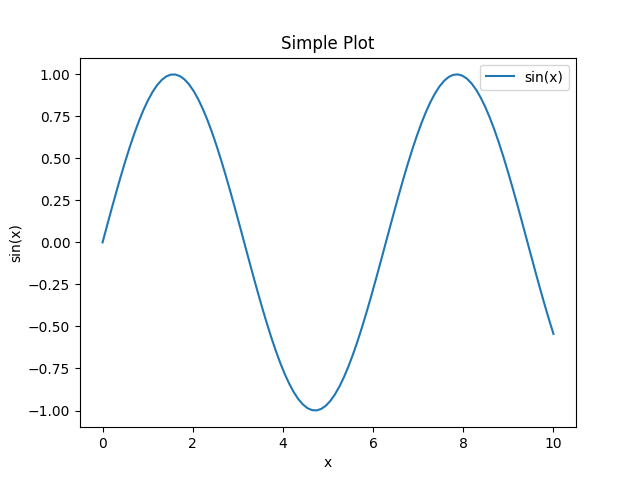
\includegraphics[width=0.8\textwidth]{203/Figure_1.png}
\end{figure}

除了使用简洁的\texttt{pyplot}以外,还可以使用面向对象风格的API来绘图,便于封装和复用:

\begin{lstlisting}
import matplotlib.pyplot as plt
import numpy as np

x = np.linspace(0, 2*np.pi, 100)  # Create x values from 0 to 2pi

fig, ax = plt.subplots(figsize=(8, 6))  # 创建一个图形和坐标轴对象
ax.plot(x, np.sin(x), label=r'$sin(x)$', color='tab:blue', lw=2)  # 绘制曲线
ax.plot(x, np.cos(x), label=r'$cos(x)$', ls='--')  # 绘制曲线
ax.set_xlabel(r'$x$')  # 添加坐标轴标签
ax.set_ylabel(r'$y$')  # 添加坐标轴标签
ax.legend()  # 添加图例
ax.set_title('Matplotlib Example')  # 添加标题
fig.tight_layout()  # 自动调整布局
plt.show()  # 显示图形
\end{lstlisting}
上述代码使用\texttt{plt.subplots}函数创建了一个图形和坐标轴对象,然后使用坐标轴对象的\texttt{plot}方法绘制曲线。这样可以更灵活地控制图形的各个部分。

\begin{figure}[ht]
  \centering
  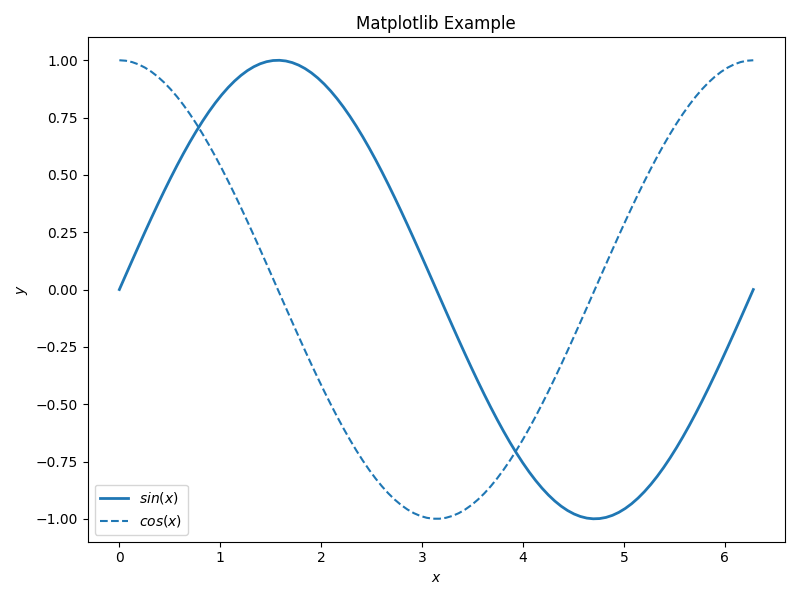
\includegraphics[width=0.8\textwidth]{203/Figure_2.png}
\end{figure}

\subsection{和其他包协同工作}

Matplotlib可以和NumPy、Pandas等库无缝集成,提供了强大的绘图功能。例如,我们可以使用NumPy生成数据,然后使用Matplotlib绘制图形:
\begin{lstlisting}
import matplotlib.pyplot as plt
import numpy as np

X, Y = np.meshgrid(np.linspace(-3, 3, 300),
                   np.linspace(-3, 3, 300))
Z = np.sinc(np.sqrt(X**2 + Y**2))

fig, ax = plt.subplots()
c = ax.contourf(X, Y, Z, levels=50, cmap='viridis')
fig.colorbar(c, ax=ax)

plt.title('Contour Plot of Sinc Function')
plt.xlabel('X-axis')
plt.ylabel('Y-axis')
plt.show()
\end{lstlisting}

\begin{figure}[ht]
  \centering
  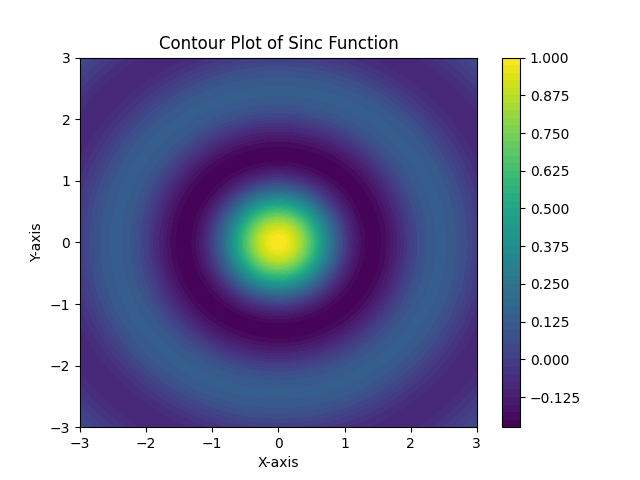
\includegraphics[width=0.8\textwidth]{203/Figure_3.png}
\end{figure}

或者使用Pandas绘制数据框的图形:
\begin{lstlisting}
import pandas as pd

df = pd.read_csv('experiment.csv')
ax = df.plot(x='voltage', y='current', kind='scatter', color='k')
ax.set_xlabel('Voltage (V)')
ax.set_ylabel('Current (mA)')
# 这只是一个示例,没有数据是真不行,后面绘图的逻辑自己写就好了
\end{lstlisting}

\subsection{子图布局}

在实际应用中,我们经常需要将多个图形绘制在同一个窗口中,这就需要用到子图的概念。Matplotlib提供了\texttt{subplot}和\texttt{subplots}函数来创建子图。

\begin{lstlisting}[language=python]
import matplotlib.pyplot as plt
import numpy as np

x = np.linspace(0, 10, 100)
y1 = np.sin(x)
y2 = np.cos(x)

fig, axs = plt.subplots(2, 1, figsize=(8, 6))  # 创建2行1列的子图
axs[0].plot(x, y1, label='sin(x)', color='tab:blue')
axs[0].set_title('Sine Function')
axs[1].plot(x, y2, label='cos(x)', color='tab:orange')
axs[1].set_title('Cosine Function')
plt.tight_layout()
plt.show()
\end{lstlisting}
上述代码创建了一个包含两个子图的图形窗口,分别绘制了正弦函数和余弦函数。\\使用\texttt{plt.tight\_layout()}函数可以自动调整子图之间的间距。

\begin{figure}[ht]
  \centering
  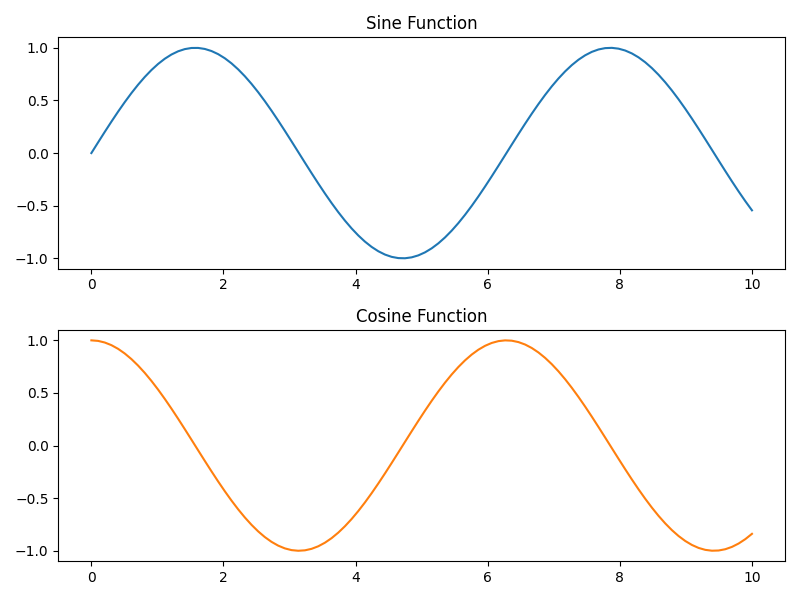
\includegraphics[width=0.8\textwidth]{203/Figure_4.png}
\end{figure}

\subsection{风格和导出}

Matplotlib支持多种风格,可以通过\texttt{plt.style.use}函数来设置风格。例如,我们可以使用\texttt{science}和\texttt{ieee}风格来绘制图形,使得图形符合IEEE论文的格式要求:
\begin{lstlisting}[language=python]
plt.style.use(['science', 'ieee'])  # 需安装 SciencePlots
\end{lstlisting}
当然,如使用该风格,则默认需要LaTeX来渲染文本,而这是非常缓慢的。因此可以在该列表中添加\texttt{no-latex}选项,以禁用LaTeX渲染:
\begin{lstlisting}[language=python]
plt.style.use(['science', 'ieee', 'no-latex'])  # 需安装 SciencePlots
\end{lstlisting}

\begin{figure}[ht]
  \centering
  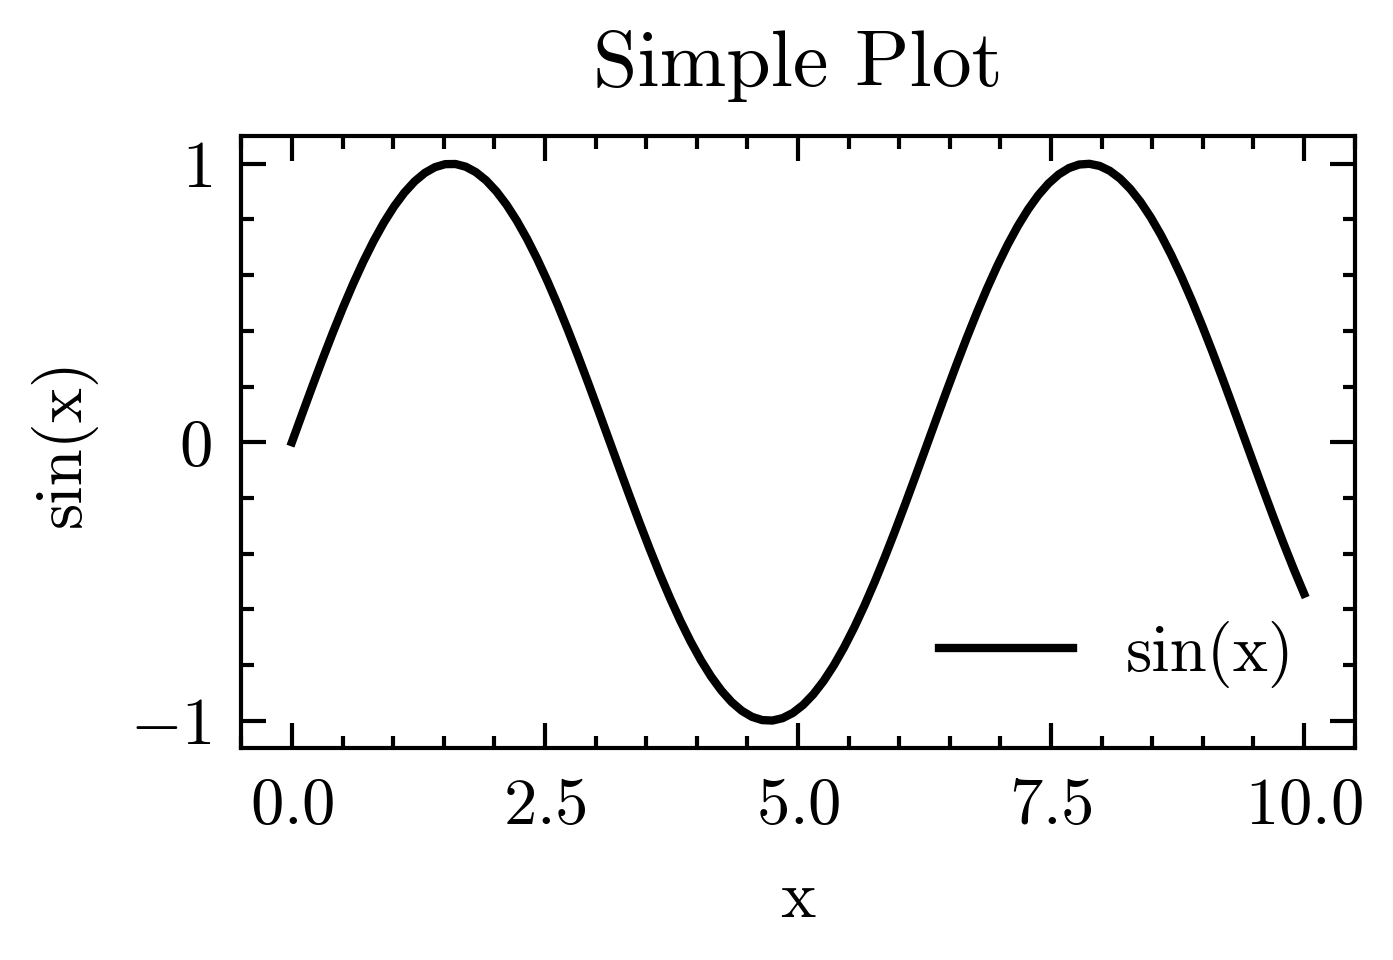
\includegraphics[width=0.8\textwidth]{203/Figure_5.png}
  \caption{使用SciencePlots风格绘制的图形}
\end{figure}

此外,我们还可以将图形导出为各种格式,如PNG等:
\begin{lstlisting}[language=python]
plt.savefig('figure.svg')   # 矢量图
plt.savefig('figure.png', dpi=600, transparent=True) # PNG图
\end{lstlisting}

\subsection{常见坑与提示}

\begin{itemize}
  \item 中文字体乱码:提前设置rcParams,或者使用\texttt{matplotlib.font\_manager}来设置中文字体。
    \begin{lstlisting}[language=python]
import matplotlib.pyplot as plt
plt.rcParams['font.sans-serif'] = ['SimHei']  # 设置中文字体
plt.rcParams['axes.unicode_minus'] = False  # 解决负号显示为方块的问题
    \end{lstlisting}
  \item 在Jupiter中不显示:使用\texttt{\%matplotlib inline}命令来确保图形在Jupyter Notebook中显示。
  \item 颜色过多:使用\texttt{tab:}前缀来使用Matplotlib内置的颜色表,避免颜色过多导致的混乱。
  \item 图例遮挡:使用\texttt{bbox\_to\_anchor}参数来调整图例的位置,或者\texttt{plt.legend(loc='best')}自动解决图例位置问题。
\end{itemize}

除此之外,Matplotlib还有许多其他的功能,如动画、3D绘图等,这些内容同学们可以在\href{https://matplotlib.org/stable/gallery/index.html}{Matplotlib官方示例}中找到。

\section{SymPy:符号计算高级计算器}

\begin{flushright}
建议本节阅读者有一定的高等数学基础。
\end{flushright}

SymPy是一个用于符号计算的Python库。符号计算是指对数学表达式进行符号操作,而不是数值计算;或者说,\textbf{求解析解而不是数值解}。SymPy可以用于求解方程、积分、微分、矩阵运算等多种数学操作。它的语法类似于Mathematica和Maple,但使用Python语言编写,因此更易于学习和使用。

在使用该库之前,我们尽量在文件的靠前位置添加下面这一行,这样可以让SymPy的输出更加美观。
\begin{lstlisting}[language=python]
  init\_printing(use\_unicode=True)
\end{lstlisting}

\subsection{基本数据类型}
SymPy的基本数据类型有三个:符号、表达式、等号。符号是SymPy的核心数据类型,用于表示数学符号,如变量、常数等。表达式是由符号和运算符组成的数学表达式,可以进行各种数学操作。等号用于表示等式关系。
\begin{lstlisting}[language=python]
    x, y = symbols('x y', real=True)  # 定义符号变量 x 和 y
    expr = x**2 + y**2  # 定义表达式
    line = Eq(y, 3*x + 2) # 定义等式
    print(expr)  # 输出表达式
\end{lstlisting}
上述代码定义了两个符号变量x和y,并定义了一个表达式$x^2 + y^2$和一个等式$y = 3x + 2$。SymPy的符号计算可以对这些符号进行各种操作,如求导、积分、化简等。

比方说:
\begin{lstlisting}
    expr = (x+1)*(x-2)-(x**2-2)
    simplify(expr)  # 化简表达式, 得到-x
    expand((x+1)**5)  # 展开多项式
    factor(x**3+1)  # 因式分解
    limit(expr, x, 0)  # 求expr在 x=0 处的极限
    diff(expr, x)  # 对 expr 求一次导数
    integrate(expr, x)  # 对 expr 求不定积分
    integrate(expr, (x, 0, 1))  # 对 expr 求定积分
    series(expr, x, 0, 5)  # 求泰勒级数展开,最高项次数为不超过4
    series(expr, x, 0, 5).removeO()  # 去掉高阶项
    solve(x**4-1, x)  # 求解等式x**4-1=0的解
    solve(a*x**2+b*x+c, x)  # 求解二次方程ax^2+bx+c=0的解,带着参数也能算
    nonlinsolve([x**2+y**2-1, x-y], (x, y))  # 求解非线性方程组
\end{lstlisting}

多元函数也可以使用上述方法来求导和积分,这里就不写了。需要注意的是,这里的求导数都是\textbf{偏导数}。一个非常有趣的事情是:在该库中,使用\texttt{-oo}和\texttt{oo}来表示负无穷和正无穷,而不是使用\texttt{float('inf')}。(疑似有些过于符号化了)

\subsection{矩阵和线性代数}
SymPy还提供了矩阵和线性代数的功能,可以进行矩阵运算、求逆、求特征值等操作。SymPy的矩阵是一个二维数组,可以进行各种矩阵运算,如加法、乘法、转置等。
\begin{lstlisting}[language=python]
    A = Matrix([[1, 2], [3, 4]])  # 定义一个矩阵
    b = Matrix([x, y])  # 定义一个列向量

    A.det()  # 求矩阵的行列式
    A.inv()  # 求矩阵的逆
    A.eigenvals()  # 求矩阵的特征值

    linsolve((A, b), [x, y])  # 求解线性方程组 Ax = b

    P, D = A.diagonalize()  # 对矩阵对角化,P为特征向量矩阵,D为对角矩阵
\end{lstlisting}

\subsection{输出、可视化}
在Jupiter里一行搞定输出,贴出来的字符串直接粘到论文里就能编译:
\begin{lstlisting}
    latex(Integral(exp(-x**2), (x, 0, oo)))
\end{lstlisting}

如果需要将表达式可视化,可以使用SymPy的\texttt{plot}函数来绘制函数图像:
\begin{lstlisting}[language=python]
    plot(sin(x)/x, (x, -10, 10))
\end{lstlisting}

\subsection{常见坑}
\begin{itemize}
  \item 符号爆炸:符号计算缓慢是正常现象,表达式也会越来越大。必要的时候,simplify、expand、factor等函数可以帮助我们化简表达式。
  \item 算错:这是常规现象,符号计算可能出现算错是不可避免的。我们可以快速使用数值验证结果的正确性。
  \item 并行:Sympy不能并行,但是可以拆任务并行计算(如multiprocessing)。
\end{itemize}

祝愿玩得开心,下次计算不用抄公式抄到手软!

\section{爬虫}

爬虫很难说是一个包。它实际上是一种技术,或者说是一种思维方式。爬虫的核心思想是:模拟浏览器行为,自动化地获取网页内容。Python中有许多用于爬虫的库,如Requests、BeautifulSoup、Scrapy等。

一般而言,爬虫的基本流程包括以下几个步骤:
\begin{enumerate}
  \item 发送HTTP请求:使用Requests库发送HTTP请求,获取网页内容。
  \item 解析网页内容:使用BeautifulSoup库解析HTML内容,提取所需的数据。
  \item 存储数据:将提取的数据存储到本地文件或数据库中。
\end{enumerate}
以下是一个简单的爬虫示例,使用Requests和BeautifulSoup库来爬取一个网页的标题:
\begin{lstlisting}[language=python]
import requests
from bs4 import BeautifulSoup
url = 'https://example.com'
response = requests.get(url)
soup = BeautifulSoup(response.text, 'html.parser')
title = soup.find('title').text
print(title)
\end{lstlisting}
上述代码发送了一个HTTP GET请求,获取了网页内容,并使用BeautifulSoup解析HTML,提取了网页的标题并打印出来。

当然,上述代码只是一个非常简单的爬虫示例,实际应用中可能需要处理更多的细节,如处理分页、模拟登录、处理JavaScript渲染等。另一方面,很多网站实际上已经做了反爬虫处理,想要成功爬取数据可能需要更多的技巧和方法。出于个人原因,笔者也很少使用爬虫技术,因此我在这里就不做过多介绍了,感兴趣的同学可以自行查找相关资料进行了解。

\begin{caution}
  爬虫涉及到法律和道德问题,爬取数据时应当遵守网站的robots.txt文件和相关法律法规,避免侵犯他人的权益。
\end{caution}

\section{OpenAI:自己做自己的Agent}

Cherry Studio等软件给了我们一个强大的图形界面,让我们可以通过各种方式来使用LLM。但是涉及到一些自动化的任务时,还是需要自己编写代码来实现。OpenAI官方提供了一个Python SDK,可以让我们方便地使用OpenAI的各种模型和功能。

实际上,OpenAI的Python SDK非常简单易用,甚至可以说是简陋到傻瓜级别的。我们如果希望使用该包,只需要记住代码分为两步:定义client,使用client。以下是一个简单的示例,使用OpenAI的GPT-4模型来生成文本:
\begin{lstlisting}[language=python]
from openai import OpenAI

API_KEY = 'your_api_key' # 这个是必须的
BASE_URL = 'https://example.com/v1'  # 请改成服务供应商提供的地址

# 定义 client
client = OpenAI(api_key=API_KEY, base_url=BASE_URL)

# 使用 client
with client.chat.completions.create(
    model='gpt-4o', # 取决于实际情况
    messages=[
        {'role': 'system', 'content': 'You are a helpful assistant.'},
        {'role': 'user', 'content': 'Hello, how are you?'}
    ] # Prompts需要自己写
    # 这里也可以添加 temperature, max_tokens 等参数
) as response:
    print(response.choices[0].message.content)
\end{lstlisting}

在上述代码中,我们首先定义了一个OpenAI客户端,然后使用该客户端发送了一个聊天请求,获取了模型的回复并打印出来。使用\texttt{with}语句可以确保资源的正确释放,是良好的习惯。

于是上述库的使用就这么简单,疑似确实是傻瓜级别的。更多的功能和用法可以参考相关文档。当然,如果希望进行记忆持久化等功能,那需要其他的库来实现,例如\texttt{langchain}和\texttt{langgraph}等。


\begin{thinking}
  以下内容是一些简单的实践选题,供同学们参考。可以使用LaTeX来形成实验报告!
  \begin{enumerate}
    \item 用《红楼梦》文本做词-人共现网络:试着读入一段红楼梦文本,统计人物和词语的共现关系,并使用SnowNLP等库为人物的情绪打分,最终观察人物的情绪走势。
    \item 用PyTorch试着复现线性回归的解析解:试着生成一百万个三维点,使用PyTorch实现线性回归,并与解析解进行对比。提示:解析解可以使用Numpy求得,公式是$w^* = (X^TX)^{-1}X^Ty$。
    \item 使用多个库做信号处理,做出一个简单的调音器:可以使用pyaudio库来辅助录音,使用SciPy来做FFT变换,使用Matplotlib来做频谱图,使用SymPy来做滤波器设计。
    \item 使用PyTorch训练一个简单的神经网络来做手写数字特征提取;然后使用UMAP来降维可视化。提示:ResNet。
    \item 混沌摆模拟:使用SciPy的ODE求解器来模拟一个混沌摆的运动轨迹,然后使用Matplotlib来绘制相空间图和时间序列图。你能做出一个动画吗?如果你有GPU,可以使用PyTorch来并行,看看混沌敏感性。
  \end{enumerate}
\end{thinking}

\chapter{实用主义编程}

现在同学们的前置知识已经充分,是时候开始正式走向开发了。

对于一些同学而言,即使他们走向工作岗位或者科研岗位之后,他们写出的代码依然难以阅读,更难以进行长期维护。从某种程度上说,\textbf{代码是写给人看的},机器只是顺便运行,按理说写成什么样子都可以;但是如果可读性太差的话,估计未来的自己都会抽自己几巴掌——完全看不懂。因此,我们将在这里介绍一下怎么才能真正写出来一些\textbf{真正可以交付}的代码。

\section{写代码的基本素养}\label{sec:code-style}

代码风格(码风)是指代码的书写规范和格式化方式。良好的代码风格可以提高代码的可读性和可维护性,使得其他人(包括未来的自己)能够更容易地理解和修改代码。一般情况下,我们会遵循一些通用的代码风格规范,例如 Google C++ Style Guide 或 PEP 8(Python Enhancement Proposal 8)等。而在团队协作的时候,我们则尽可能保证码风和团队的码风一致。

\subsection{通用代码风格指南}

尽管不同语言和项目有不同的风格,但以下几点是相对普适的、值得注意的基本素养:
\begin{itemize}
  \item \textbf{缩进}:使用空格或制表符进行缩进,通常使用2个空格或4个空格或1个制表符。关键是 \textbf{不要混用} 空格和制表符。
  \item \textbf{命名}:使用有意义的变量名(\texttt{int user\_count})和函数(\texttt{calc\_total\_price()}),不要使用单个字母(\texttt{a1})、过度缩写(\texttt{cal()})或无意义的名称(\texttt{tmp1})。此外,在同一个项目中,对于同一种程序实体(例如,类、函数、变量),应当采用统一的命名风格。例如大驼峰(CamelCase)、小驼峰(camelCase)、下划线(snake\_case)等。绝大多数时候,常量通常使用全大写字母和下划线分隔(例如\texttt{MAX\_VALUE})。
  \item \textbf{注释}:在代码中添加适当的注释,解释代码的逻辑和意图。注释应该简洁明了,不要过于冗长。同时,注释应该与代码保持同步,避免出现过时的注释。避免使用\texttt{\#if 0}和\texttt{\#endif}来注释代码,这种方式风格很老,现在已经不推荐使用了。
  \item \textbf{空行}:适当使用空行来分隔代码块,以提高可读性。通常在逻辑相关的代码块之间、函数之间、类之间使用一到两个空行。
  \item \textbf{括号}:使用一致的括号风格,例如 K\&R 风格(函数定义的左括号在同一行)或 Allman 风格(函数定义的左括号在新的一行)。
  \item \textbf{空格}:在运算符两边添加空格,例如\texttt{a + b}而不是\texttt{a+b}。在逗号、分号等符号后面添加空格,例如\texttt{a, b}而不是\texttt{a,b}。
  \item \textbf{行长度}:尽量保持每行代码的长度在80-120个字符之间,避免过长的行导致代码难以阅读。
  \item \textbf{文件长度}:尽量保持每个文件的长度在合理范围内(例如不超过1500行),避免过长的文件导致代码难以阅读和维护。
\end{itemize}

\subsection{特定语言与社区风格指南}

代码风格并非放之四海而皆准的真理。不同的编程语言、社区和公司都有自己独特的代码风格规范。无论是开源社区项目还是公司内部项目,当你参与时,都应该优先遵循其既有的代码风格。这有助于你更好地融入团队,并与他人高效协作。

以下是一些常见语言的知名代码风格指南,可供参考:

\subsubsection{Python: PEP 8}
Python社区广泛遵循\href{https://www.python.org/dev/peps/pep-0008/}{PEP 8}(Python Enhancement Proposal 8)规范。它对命名约定、缩进、行长度、注释格式等都做了详细规定。PEP 8推荐使用4个空格进行缩进,函数和变量名使用下划线命名法(snake\_case)。

\subsubsection{C: K\&R, GNU, and Linux Kernel Style}
作为一门历史悠久的系统编程语言,C语言形成了多种常见的代码风格。
\begin{itemize}
  \item \textbf{K\&R风格}:源自C语言的作者Brian Kernighan和Dennis Ritchie的\href{https://en.wikipedia.org/wiki/The_C_Programming_Language}{著作}\textsc{The C Programming Language}。它的特点是括号风格紧凑,左大括号跟在函数名或控制语句的同一行。这是许多后续风格的基础。
  \item \textbf{GNU风格}:由\href{https://www.gnu.org/prep/standards/standards.html}{GNU项目}推广。它对代码的布局和注释有非常详细的规定。其括号风格很独特,大括号需要单独成行并缩进。
  \item \textbf{Linux内核风格}:由Linus Torvalds主导,用于\href{https://www.kernel.org/doc/html/latest/process/coding-style.html}{Linux内核的开发}。它基于K\&R风格,但有自己独特的规则,例如使用制表符(tab)进行缩进(且一个tab等于8个空格),并严格限制行长为80个字符。
\end{itemize}

\subsubsection{C++: Google Style Guide \& LLVM Style}
C++ 社区存在多种代码风格。其中,\href{https://google.github.io/styleguide/cppguide.html}{Google C++ Style Guide} 是一个非常著名且详尽的指南,被广泛应用于Google内部及其开源项目。它规定了包括文件命名、类设计、函数参数顺序在内的方方面面。另一个有影响力的风格是 \href{https://llvm.org/docs/CodingStandards.html}{LLVM Coding Standards},它在开源编译器社区中非常流行。

\subsubsection{关注项目与社区习惯}
即便是相对小众的语言,其社区也往往会形成自己的代码风格。例如,Vala语言的社区就有一套流行的\href{https://docs.elementary.io/develop/writing-apps/code-style}{elementary编码风格},它在函数调用时推荐在函数名和括号间加空格(例如\texttt{print ("Hello");}),这与许多其他语言的习惯可能不同。

当你加入一个新项目时,至关重要的第一步往往是花时间阅读并理解其代码风格指南。如果项目没有成文的规范,那么就通过阅读现有代码来学习和模仿其风格。\textbf{保持一致性是关键,不要将个人偏好随意带入项目中。}这不仅是对项目和其他贡献者的尊重,也能让你的代码更快地被他人接受。

\subsubsection{自动化工具的重要性}
我们自己写代码的时候虽然不能强制要求自己遵循某种风格,但是在团队协作中,保持一致的代码风格是非常重要的。我们可以使用一些工具来自动格式化代码,VS Code的C++插件就提供了代码格式化功能,可以通过快捷键(通常是Shift + Alt + F)来自动格式化代码。至于python,我们\texttt{pip install black},然后\texttt{black .}就可以自动格式化当前目录下的所有python文件了。

不要什么都手动缩进。人类不是打字机,机器比我们人打的整齐十倍甚至九倍。

除了这些以外,不同的岗位也有一些不同的码风需求,例如对于后端而言一个非常常见的差代码:
\begin{lstlisting}[language=C++]
    for(int i = 0; i<s.length(); i++){
        if(s[i] == 'a'){
            s[i] = 'b';
        }
    }
\end{lstlisting}
以上代码的意图是将字符串中的所有字母a替换为b,但是它的效率非常低下,因为每次替换都需要调用一遍\texttt{s.length()},而且每次替换都需要重新构建字符串,前端得等半天才能看到结果。而前端也有可能出现类似错误,前端的差代码可能是把SQL语句写进了HTML中,这直接导致了SQL注入漏洞,后端同学估计会直接气炸。

为了规避这些错误,同学们需要在实际项目中不断积累经验,才能写出更好的代码。

\subsection{注释}

很多人都不喜欢写注释,认为代码本身就应该是自解释的,实则不然。当代码逻辑复杂或者涉及到一些特定的业务逻辑时,注释就显得尤为重要;要是码风再差一点,代码就更不能自解释了。

于是我们赌气一般地写了以下注释:
\begin{lstlisting}[language=Python]
    i += 1  # 增加 i 的值
\end{lstlisting}

对以上注释,我的看法是不如不写,因为只要是认识 \texttt{+=}的人都知道这行代码的意思,这句话本质上是在重复代码本身,没有什么用处。

因此,注释的原则是:\textbf{注释应该解释代码的意图},或者说,\textbf{说清楚为什么这么写(在做什么)}而不是“这是什么”。或者举个例子:

\begin{lstlisting}[language=Python]
    i += 1 # 跳过表头行,数据从下一行开始
\end{lstlisting}

这行注释就比上面的注释有用得多,后续在做代码评审的时候也很容易复现当时的思路。

当然,我们作为汉语使用者不喜欢注释非常正常,因为谁都不喜欢来回切输入法,我也不喜欢大量的写注释。但是对于一些复杂的逻辑,虽然无法要求自己每一行都写注释,但是至少要在关键的地方写注释,例如某个非常复杂的算法,至少也要按照步骤写注释(这一部分是做什么,那一部分是做什么)。

\begin{note}
  部分公司做自建库的时候,会强制要求代码中注释达到一定的比例。这本意是好的,但是如果注释的质量不高,反而会导致代码难以阅读。部分人甚至导入数万字的网文来应付了事,这是非常不推荐的。
\end{note}

\section{防御式编程}

近年来防御式编程已经被解构成一个令人不忍直视的名词,例如向代码中添加大量的逆天处理(例如\texttt{\#define true false})来防止自己被其他人取代或者被公司裁员。这完全是违背了“防御式编程”的初衷,这个名词来源于防御式驾驶,也就是你永远不知道其他司机会干出什么妨碍你的事来,所以要保持警惕。同理,在编程的时候也要保留着大量的警惕,防止别人或者自己在未来时犯错误;同时也在代码崩溃的时候把本不属于自己的错误优雅地甩锅给别人。

除了最常见的大量\texttt{if-else}以外,我们还可以使用一些其他的手段来更优雅地实现防御式编程,例如使用异常处理机制(try-catch)来捕获错误,或者使用断言(assert)来检查代码的前置条件和后置条件。

\subsection{异常处理}

程序员中经常流传着一首歌曲(尤其是C\#程序员):“死了都要Try……”\footnote{来自著名歌曲《死了都要爱》},说明了异常处理机制的重要性。异常处理机制可以帮助我们捕获和处理运行时错误,避免程序崩溃;换句话说,异常处理机制的思路是“晚崩溃,晚挨骂”。

一个经典的C\#异常处理结构如下:
\begin{lstlisting}
    try{
        // 可能有毛病的代码
        // 我们甚至可以人造异常
        // 例如throw new Exception("这是一个人造异常");
    }
    catch(Exception e){
        // 出了毛病就执行的代码,例如打印错误信息
    }
    finally{
        // 无论如何都会执行的代码
    }
\end{lstlisting}

一般finally可以省略,在其他语言中语法也差不多。一个示例是:
\begin{lstlisting}[language=Python]
try:
    user = User.get_by_id(user_id)
except UserNotFoundError:
    logger.error(f"用户{user_id}不存在")
    return {"error": "用户不存在"}
\end{lstlisting}

这种代码在查询的时候非常常见,能够有效地防止查到空对象并尽早暴露问题,同时还能防止程序崩溃,防止笨蛋甲方在酒吧点炒饭的时候不停地输入不存在的用户ID导致程序崩溃。

\begin{caution}
  不要滥用异常处理机制,尤其是写出这种代码:\texttt{except Exception as e: pass},除非你这个大笨蛋想被运维半夜叫醒。
\end{caution}

\subsection{断言}

断言的意思是“我认为这个应该是对的”,如果不成立就抛出异常。断言通常用于检查代码的前置条件和后置条件,确保代码在运行时满足一定的条件。断言可以帮助我们在开发阶段发现问题,并且在生产环境中也可以用来捕获一些潜在的错误。断言的思路和异常处理的思路是相反的:早崩溃,早开心。

比方说以下代码:

\begin{lstlisting}[language=Python]
def divide(a, b):
    return a / b
\end{lstlisting}

然后某在酒吧点炒饭的笨蛋甲方输入了0作为第二个参数,导致程序崩溃,然后甲方开骂,乙方只能默默挨骂。

这时候,我们可以使用断言来解决这个问题:
\begin{lstlisting}[language=Python]
def divide(a, b):
    assert b != 0, "除数不能为零!"
    return a / b
\end{lstlisting}

如果甲方输入了0作为第二个参数,程序就会抛出异常(一个“断言错误”),并且输出“除数不能为零!”的错误信息。这样就可以避免程序崩溃,并且可以更好地定位问题。(甲方估计也不会因为这个错误而开骂了)

这个代码如果用raise来写的话就会变成:
\begin{lstlisting}[language=Python]
def divide(a, b):
    if b == 0:
        raise ValueError("除数不能为零!")
    return a / b
\end{lstlisting}
\texttt{raise}是Python中手动抛出异常的语句,和C\#的\texttt{throw}很像。上述代码和使用断言的区别有两点:一个是代码量变大了(多了一行,不够优雅),另一个是这个异常抛出的是“值错误”而不是“断言错误”。不过在实际操作中,这两个区别不大,且在查询等需要更多信息的场景中,使用\texttt{raise}会更好一些(生产环境中往往禁用断言,优雅不能当饭吃)。

在C系中,也有这样的断言,包括运行时断言和编译时断言。运行时断言指的是在运行时会检查某些条件是否成立,对编译进程没有影响;编译时断言则是在编译阶段就检查某些条件是否成立,如果不成立直接掐断编译。

下文是一个运行时断言:
\begin{lstlisting}[language=C]
#include <assert.h>
void divide(int a, int b) {
    assert(b != 0 && "除数不能为零!");
    printf("%d\n", a / b);
}
\end{lstlisting}

\section{监控程序的运行情况}\label{sec:monitoring}

\subsection{日志}\label{subsec:logging}

日志能够帮助我们记录程序运行时的状态和错误信息,我们在\ref{subsec:debugging}节中提到过的“打日志”调试方式就是一种使用日志的方式。

使用print语句是很初级的一种打日志手段,通常我们还会使用更高级的日志库,例如Python的logging模块或者C++的spdlog库等。这些日志库可以提供更丰富的功能,例如日志级别、日志格式化、日志输出到文件等。使用这些日志库可以让我们的代码更加优雅,同时也能更好地管理日志信息。通常说来,日志有以下几个级别(严重性从低到高):
\begin{itemize}
  \item \textbf{DEBUG}:调试信息,通常用于开发阶段,记录一些调试信息。
  \item \textbf{INFO}:普通信息,记录一些程序运行的基本信息。
  \item \textbf{WARNING}:警告信息,记录一些可能导致问题的情况,但不影响程序的正常运行。
  \item \textbf{ERROR}:错误信息,记录一些导致程序无法正常运行的错误。(这些错误往往不会导致程序崩溃)
  \item \textbf{CRITICAL}:严重错误信息,记录一些导致程序崩溃的错误。
\end{itemize}

日志通常遵循一定的结构:时间-模块-级别-消息。例如:
\begin{lstlisting}
    2025-07-16 14:30:00 [user.py:45] ERROR 用户123登录失败:密码错误
\end{lstlisting}

日志的格式化可以使用一些工具来实现,例如Python的logging模块提供了丰富的格式化选项,可以自定义日志的输出格式。

\subsection{其他监控手段}\label{subsec:other-monitoring}

除了日志,我们还可以使用其他的监控手段来监控程序的运行情况,比方说打开任务管理器,查看CPU、GPU、内存等资源的使用情况;或者使用一些性能分析工具,例如Python的cProfile模块、C++的gprof工具等,来分析程序的性能瓶颈;特定领域也有一些特定的性能分析工具,例如TensorBoard等。

一个例子:我们在机器学习相关的课程实验中经常会遇到训练过慢的问题。这个时候,不妨打开任务管理器,重点查看GPU和内存的使用情况。如果GPU使用率很低,要么是代码没有充分利用GPU的计算能力,应该增加并行能力(如提高批量大小)以加快代码运行速度;要么是代码没有在GPU上运行,这时候应该检查代码是否有从CPU到GPU的数据传输等。如果GPU使用率很高,说明代码可能存在性能瓶颈或者数据处理不当的问题,应该降低并行程度(但是一般这很难遇见,毕竟这种情况下可以堆卡)。如果内存使用率很高,说明代码可能存在内存泄漏或者数据处理不当的问题。通过这些信息,我们虽然很难直接定位代码的问题所在,但是也可以得到一些直接或者间接的线索,从而更好地优化代码。

对于一些使用HTTP服务的项目,我们还可以监控服务的请求和相应情况,其中最重要的数据应该是QPS(每秒请求数)和响应时间。如果QPS很低或者降到0,说明服务大概率出现了问题(另一种可能是真没有人使用这个服务);如果响应时间很高,说明服务可能存在性能瓶颈或者数据处理不当的问题。我们可以使用一些工具来监控服务的请求和响应情况,例如Prometheus、Grafana等。前端的开发人员也可以使用浏览器自带的开发者工具来监控页面的加载时间、资源使用情况等。

\section{常见的代码架构}\label{sec:code-architecture}

在实际的开发中,为了便于组织代码,我们通常会遵循一定的代码架构,而不是把代码这碗面煮成一锅粥或者面疙瘩汤。在这里,我们向大家介绍几个常见的架构:

\subsection{MVC架构}

这可以说是最简单的代码架构之一了。它由三个相对独立但是联系密切的部分组成:模型(Model)、视图(View)和控制器(Controller)。模型负责数据的存储和处理,视图负责展示用户界面,控制器负责处理用户输入、协调模型和视图之间的交互。

举个例子:假设我们在制作一个视觉小说游戏,那么我们的代码架构可以采取以上架构:
\begin{itemize}
  \item 模型:负责存储游戏的状态、角色信息、剧情分支等数据。
  \item 视图:负责展示游戏的界面,包括角色立绘、背景、对话框等。
  \item 控制器:负责处理用户的输入,例如点击选项、输入文本等,并根据用户的选择更新模型和视图。
\end{itemize}

MVC架构的优点是将代码分成了三个相对独立的部分,实现起来非常简单,尤其适用于中小型项目。缺点是三个部分之间虽然有着明确的职责划分且相对独立,但是耦合度仍然较高,如果需要修改某个部分的代码,经常会影响到其他部分的代码(你一改代码,别人都得跟着改),代码的可维护性比较低。

\subsection{MVVM架构}
MVVM(Model-View-ViewModel)架构是一种常用于前端开发的架构,它将视图(View)和业务逻辑(ViewModel)分离开来,从而实现了更好的代码组织和可维护性。MVVM架构通常用于前端框架,例如Vue.js、Angular等。笔者不是前端程序员,对MVVM了解甚少,于是不在这里误人子弟了。感兴趣的同学可以自行查阅相关资料。

\subsection{洋葱架构(干净架构)}

洋葱架构(也叫干净架构)是一种分层的架构,它的“层”之间有着严格的依赖关系。一般而言,洋葱架构分四层,外层依赖内层,但内层对外层一无所知,没有任何依赖。

一个典型的洋葱架构分四层:
\begin{itemize}
  \item \textbf{实体层(Entity Layer)}:最内层,包含业务逻辑和领域模型。它定义了系统的核心业务规则和数据结构。
  \item \textbf{用例层(Use Case Layer)}:第二层,包含应用程序的用例和业务逻辑。它定义了系统的功能和行为,并调用实体层来实现业务逻辑。
  \item \textbf{接口层(Interface Layer)}:第三层,包含与外部系统交互的接口和适配器。它定义了系统的输入和输出,并调用用例层来实现功能。
  \item \textbf{外部层(External Layer)}:最外层,包含与外部系统交互的具体实现,例如数据库、Web服务等。它依赖接口层来实现功能。
\end{itemize}

洋葱架构的优点是将代码分成了四个仅单侧依赖的部分,代码的可维护性和可扩展性都比较高(换UI不用动数据库格式;换数据库不用动业务逻辑)。缺点是实现起来比较复杂,因此比较适用于大型项目。如果同样拿刚刚的视觉小说游戏来举例,那么我们的代码架构可以采取以上架构:
\begin{itemize}
  \item 实体层:定义游戏的状态、角色信息、剧情分支等数据结构。
  \item 用例层:处理游戏的逻辑,例如实现判断玩家的选择、更新游戏状态、计算好感度等方法,但是不关心其他层怎么用这玩意。
  \item 接口层:与外部系统交互,例如接受点击的信息后,调用某个方法、返回某些数据,但不关心这数据具体是JSON还是SQL。
  \item 外部层:负责具体的实现。
\end{itemize}
这样,故事脚本永远在最甜的心里,就算明天把Unity改成Godot、把这个立绘换成那个立绘,也只需要替换最外层,里面一点不用动。但是这样既不够直观,也不够简单,反而会让人觉得过于臃肿、没有必要。

但是如果我们要做一个类似于微信的即时通讯软件,那么洋葱架构就非常适合了:
\begin{itemize}
  \item 实体层:定义用户信息、聊天记录等数据结构,别的啥也不干。
  \item 用例层:基于这些数据结构,处理核心的业务逻辑,例如处理好友关系、群成员上限判断、雪花算法、端到端加密策略等,并不关心接口层用这些玩意干什么。
  \item 接口层:使用用例层给出的方法,处理用户输入和输出,例如收到“发送消息”事件$\rightarrow$检查权限$\rightarrow$端到端加密算法$\rightarrow$发送到服务器$\rightarrow$返回“发送成功”事件。它只关心如何使用用例层提供的功能,而不关心其他层具体怎么搞的。
  \item 外部层:负责具体的实现,包括并不限于在手机上、电脑上、车载系统上等不同平台的实现。
\end{itemize}

这样,把聊天核心逻辑(内两层)做成一个独立 SDK,外层壳子可以是微信本体、企业微信、微信 Mac 客户端,甚至车载微信,可移植性非常强。这样拆完,需求变更、团队并行、平台移植都变得像剥洋葱——泪流满面的是甲方,不是程序员。

\subsection{微服务架构}

与以上的架构不同,微服务架构并没有一个非常统一的部分或者层次划分;它的宗旨是将一个大型项目拆成许多小的、独立度极高的服务,使得每个服务都可以独立部署、独立扩展、独立维护。每个服务都可以使用不同的技术栈和编程语言来实现,从而实现了更好的灵活性和可扩展性,适合各类大中小型项目。

微服务架构的核心是API(应用程序编程接口),每个服务都提供一组API供其他服务调用。服务之间通过API进行通信,通常使用HTTP或消息队列等方式。打个比方:一个校园,我们把它拆成了许多服务,例如教务、食堂等;我们学生(也是一个服务)可以调用各种API(例如食堂提供的“吃饭”API、教务提供的“上课”API等)来达到自己的目的。

微服务架构的缺点也很明显:服务之间的通信和协调比较复杂,需要使用一些工具来管理服务的依赖关系和通信(例如通信过多的时候就“暂时不能给你明确的答复”);另一个问题是服务之间通信的延迟、网络问题会显著降低该架构的性能和可靠性;除此之外,它还有部署复杂、测试困难等问题。

\section{Vibe Coding}

Vibe Coding(氛围编程)是一种利用AI Agent来辅助编程的方式。它的核心思想是将编程任务拆分成许多小的、独立的子任务,然后使用AI Agent来完成这些子任务,从而实现了更高效、更智能的编程方式。人类程序员在这种时候只需要对任务进行规划、对过程进行监督、对结果进行验证即可。对于有一定编程基础的同学而言,Vibe Coding可以大大提高编程效率,减少重复劳动,从而让他们有更多的时间和精力去思考和解决更复杂的问题。

\begin{caution}
  Vibe Coding对于初学者并不友好,因为初学者往往连基本的编程语法都不懂,更别说对任务进行规划、对过程进行监督、对结果进行验证了。虽然初学者的任务往往非常简单,Vibe Coding可以很轻松地完成,但是初学者并不能从中学到什么东西,反而会让他们对编程产生误解,认为编程就是让AI来做的事情,从而失去学习编程的兴趣和动力。因此,笔者并不推荐初学者使用Vibe Coding,而是建议他们先掌握基本的编程技能,然后再考虑使用Vibe Coding来辅助编程。
\end{caution}

一个最简单的Vibe Coding例子是使用ChatGPT来生成代码。例如,我们可以向ChatGPT输入以下提示:
\begin{lstlisting}
请帮我写一个Python函数,计算两个数的和。
\end{lstlisting}

而稍微复杂一些的例子:例如想写一个小的程序,使用MVC架构,并且使用Flask框架来实现一个简单的Web应用程序。我们可以向ChatGPT输入以下提示:
\begin{lstlisting}
请帮我写一个使用MVC架构的Flask Web应用程序,包含以下功能:
1. 用户注册和登录
2. 用户可以发布文章
3. 用户可以查看文章列表
4. 用户可以查看文章详情
请帮我写出代码文件结构和框架即可,不必写出具体的业务逻辑。
# ----- 分割线 -----
请帮我写出XXX文件的代码,实现XXX业务逻辑。
\end{lstlisting}
当然,在Vibe Coding的时候,一定要尽可能地把原先的代码都贴出来,并且把你想要实现的功能描述清楚。否则,AI Agent很可能会给出一些不符合你预期的代码,从而导致你需要花费更多的时间和精力去修改和调试代码。不过宁可多花时间调试代码,也不要把代码写成一锅粥。

现在的LLM大多集成了“项目”功能,使得我们可以把代码文件直接上传到LLM中,然后让它帮我们分析和修改代码,这样就更方便了。对于不支持项目功能的LLM,也可以使用一些现成的Agent,例如VS Code的插件\texttt{CLine}等,来实现类似的功能。只不过该类Agent是需要持有者的API Key的。
\chapter{调试、测试和部署}

我们在前面的章节中已经知道,代码中出现错误是难免的事情。无论是语法错误、语义错误,还是不能称得上错误但是不符合预期的行为,我们都需要进行调试和测试来找出问题所在。

一些大公司专门有“测试工程师”这类岗位来负责代码正式上线之前的测试工作,以检查代码的正确性和可靠性;但是对于大多数小型项目而言,这些工作往往是由开发人员自己完成的。在本章节中,我们会介绍一些常用的调试和测试方法,帮助同学们更好地理解和解决代码中的问题。

总得说来,调试和测试就像诊治一个危重病人(值得庆幸的是,这个病人能够复活)一样。此时,我们需要四步走:先救命、再治病、再调养,最后购买医疗保险,然后让他去工作。顺序不要乱,一步都不能少。

\section{先救命}

最常见的情况是:代码崩溃了,程序完全无法执行。对于Python而言,它的报错信息非常详细,通常可以直接定位到出错的行数和错误类型,因此往往只需要根据报错信息进行修复即可。

而对于C/C++这类语言而言,它们是静态的,运行时错误能过编译,而且它们的报错信息通常非常简洁,仅凭报错信息很难定位到具体的错误地点。因此,我们需要使用一些调试工具来帮助我们定位错误。

什么,你问我怎么确定编译错误?我认为编译错误应该由编译器来判断,而不是我们来判断;编译过一次以后,你的代码编辑器应该也能够显示哪里有编译错误!

\subsection{使用调试器}

我们在开发的过程中可以使用VS Code调试器,但是有时候我们无法获取程序源码。在这种情况下,我建议同学们使用那个最经典的调试工具——\texttt{gdb}。它是GNU项目的一部分,支持多种编程语言,包括C、C++、Fortran等。当然对于一些会读汇编的同学们而言,我觉得可以用objdump这类反汇编器来反汇编程序,并对这些汇编代码进行阅读;常见的反汇编器还有著名的IDA Pro,它是一个商业软件,价格很贵,但是功能绝对对得起它的价格:它甚至能够对反汇编出来的东西进行自动分析!
\begin{lstlisting}[language=bash]
    objdump -d ./your_program > asm.s
\end{lstlisting}

当然大多数人是没这个能力也没这个毅力去读汇编的,因此GDB最终还是我们最常用的动态调试工具。例如,以下命令可以启动GDB并加载程序:
\begin{lstlisting}[language=bash]
    gdb ./your_program
\end{lstlisting}

在GDB中,我们可以使用以下命令来设置断点、运行程序、查看变量等:
\begin{itemize}
  \item \texttt{break}:设置断点,可以简写为\texttt{b},例如\texttt{break main}在\texttt{main}函数处设置断点。也可以在特定的某一行设置断点,例如\texttt{break 42}在第42行设置断点;也可以利用偏移量来设置断点,例如\texttt{break +10}在当前行的往前数10行设置断点。
  \item \texttt{run}:运行程序。可以简写为\texttt{r}。
  \item \texttt{next}:执行下一行代码,可以简写为\texttt{n}。如果当前行是函数调用,则不会进入函数内部,而是把这个函数视为一个整体往下执行一行。该命令有一个变体\texttt{ni},它是汇编级别的断点定位,也就是执行下一条汇编指令。
  \item \texttt{step}:也是执行下一行代码,可以简写为\texttt{s}。如果当前行是函数调用,则会进入函数内部,逐行执行函数内部的代码。\texttt{si}是它的变体,表示汇编级别的单步执行。
  \item \texttt{continue}:继续运行直到下一个断点,可以简写为\texttt{c}。
  \item \texttt{print}:打印变量的值,例如\texttt{print variable},可以简写为\texttt{p variable}。如果变量是一个结构体或类的实例,可以使用\texttt{print variable.field}来打印某个字段的值。
  \item \texttt{backtrace}:查看函数调用栈,可以简写为\texttt{bt}。这对于定位程序崩溃时的调用路径非常有用。
  \item \texttt{layout}:切换到图形界面模式,可以使用\texttt{layout src}来显示源代码,使用\texttt{layout asm}来显示汇编代码。
  \item \texttt{info}:查看程序的状态,例如\texttt{info breakpoints}查看断点信息,\texttt{info registers}查看寄存器状态,\texttt{info locals}查看局部变量等。
  \item \texttt{watch}:设置观察点,当某个变量的值发生变化时暂停执行,例如\texttt{watch variable}。这对于调试复杂的逻辑错误非常有用。
  \item \texttt{set}:强制设置变量的值,例如\texttt{set variable = value}。这对于调试时修改变量的值非常有用。
  \item \texttt{list}:查看源代码(带行号),可以简写为\texttt{l}。
  \item \texttt{quit}:退出GDB。
\end{itemize}

当然,如果想要显示行号的话,我们编译代码的时候需要加上\texttt{-g}选项,例如:
\begin{lstlisting}[language=bash]
    gcc -g -o your_program your_program.c
\end{lstlisting}
也只有加上了\texttt{-g}选项,GDB才能够显示源代码和行号,\texttt{s}和\texttt{n}命令才能够逐行执行源代码,但是\texttt{si}和\texttt{ni}命令仍然能够正常执行。

以上命令其实很复杂,需要同学们多加练习才能熟练掌握。这里我推荐一个GDB的小练习:CMU ICS Lab2:BombLab。这个练习的目的是让同学们通过GDB来调试一个被加密的程序,找到正确的输入来“拆弹”。这个练习非常有趣,而且可以帮助同学们熟悉GDB的使用。

当然,GDB的TUI界面还是太老了,我推荐装个插件\texttt{pwndbg},它可以让GDB的TUI现代化得多。

\subsection{尸检}

有时候程序确实崩了,救不活了,这时候我们需要“死后验尸”,确定程序真正的“死因”。当然,我们在解剖尸体之前,至少得对死因了解个大概,例如是段错误、内存泄漏、未定义行为,还是什么奇奇怪怪的东西。

\subsubsection{段错误}

段错误可以使用core dump来分析。core dump是程序崩溃时操作系统生成的一个文件,包含了程序的内存状态和寄存器状态等信息。我们可以使用GDB来分析core dump文件。

\texttt{ulimit -c unlimited}命令可以设置core dump文件的大小限制为无限制。然后运行崩溃的程序,等着程序再崩溃一次。然后运行:\texttt{gdb ./your\_program core}。这会加载core dump文件,并且可以使用\texttt{bt}命令查看函数调用栈,使用\texttt{info locals}查看局部变量等。

\subsubsection{内存泄漏}

内存泄漏可以使用Valgrind来分析。Valgrind是一个开源的内存调试工具,可以检测内存泄漏、未初始化内存读取等问题。使用Valgrind非常简单,只需要在运行程序时加上\texttt{valgrind}命令即可,例如:
\begin{lstlisting}[language=bash]
    valgrind --leak-check=full ./your_program
\end{lstlisting}

Valgrind会输出内存泄漏的详细信息,包括泄漏的内存地址、大小、调用栈等信息。我们可以根据这些信息来定位内存泄漏的代码。

Valgrind跑完以后别急着关,如果是开源项目或者协作项目,把definitely lost那行抄下来贴到issue上面,省得以后再犯同样的错误。

\subsubsection{未定义行为}

越界和未定义行为可以使用ASan和UBSan来分析。ASan(AddressSanitizer)是一个内存错误检测工具,可以检测越界访问、使用后释放等问题。UBSan(UndefinedBehaviorSanitizer)是一个未定义行为检测工具,可以检测整数溢出、空指针解引用等问题。

我们在编译文件的时候,可以加上\texttt{-fsanitize=address}和\texttt{-fsanitize=undefined}选项来启用ASan和UBSan。

\section{再治病}

有些时候,程序没有崩溃的风险,但它的执行不符合预期且占用了过多的资源。这时候,我们需要进行性能调优和资源使用分析。以下是一些常见的性能问题和资源使用问题,以及相应的分析工具。

\subsection{CPU占用过高}

这种情况可以使用perf来分析问题,由Linux内核提供。只需要在运行程序时加上\texttt{perf}命令即可,例如:
\begin{lstlisting}[language=bash]
    perf record -g ./your_program && perf report
\end{lstlisting}

\subsection{内存占用过高}

这种情况可以使用massif来分析问题,该工具由Valgrind提供。例如:
\begin{lstlisting}[language=bash]
    valgrind --tool=massif ./your_program
\end{lstlisting}

运行完毕后,可以使用\texttt{ms\_print}命令来查看内存使用情况,例如:
\begin{lstlisting}[language=bash]
    ms_print massif.out.<pid>
\end{lstlisting}

\subsection{IO卡死}

IO卡死通常是因为程序在等待某个IO操作完成,例如网络请求、文件读写等。我们可以使用iotop来分析IO卡死问题,只需要:
\begin{lstlisting}[language=bash]
    sudo iotop -o
\end{lstlisting}
然后盯着它看,找谁疯狂IO就可以了。

当然,对于Node.js和Python服务,可以使用\texttt{--inspect}模式;然后打开Chrome浏览器,输入\texttt{chrome://inspect},火焰图和前端一样香。

\section{再调养}

经过以上的两步骤,我们总算是把程序的主要问题解决了个差不多。但是,为了保证程序的稳定性和可靠性,我们还需要进行一些额外的调养工作——测试。

\subsection{隔离}

我们最好是找个地方把需要测试的代码隔离开来,放到一个单独的地方,防止其他代码或者文件影响测试结果;对于服务类型的项目,则更是如此。我们可以使用tmux、screen或者Docker来隔离测试环境。

\subsubsection{使用tmux和screen}

tmux和screen是两个常用的终端复用工具,可以在一个终端中创建多个会话,方便我们进行隔离测试。使用方法非常简单,只需要在终端中输入\texttt{tmux}或\texttt{screen}即可进入一个新的会话。

在tmux中,我们可以使用以下命令来创建新的窗口、分割窗口等:
\begin{lstlisting}
    tmux new session -s session_name # 创建一个新的会话
    tmux ls # 列出所有会话
    tmux attach -t session_name # 连接到指定的会话
\end{lstlisting}
会这三个就行。在screen中的相同功能命令是:
\begin{lstlisting}
    screen -S session_name # 创建一个新的会话
    screen -ls # 列出所有会话
    screen -r session_name # 连接到指定的会话
\end{lstlisting}

\subsubsection{使用Docker}

docker和上述两个东西不太一样。上述两个东西只能做到“守护终端”,但是对于环境的变化无能为力。而使用docker可以做到隔离环境,甚至可以做到“守护进程”。我们可以使用Docker来创建一个隔离的测试环境,例如:
\begin{lstlisting}[language=bash]
    docker run -it --rm -v $(pwd):/app -w /app python:3.9 bash
\end{lstlisting}
以上代码的含义是创建一个Python 3.9的Docker容器,并将当前目录挂载到容器的/app目录下,然后进入容器的bash终端。这样,我们就可以在隔离的环境中进行测试了。上述命令中,\texttt{-it}表示交互式终端,\texttt{--rm}表示容器退出后自动删除,\texttt{-v}表示挂载目录,\texttt{-w}表示设置工作目录。如果我们不希望容器退出后自动删除,可以去掉\texttt{--rm}选项。当然,上述命令还是太长了,我们往往写成一个脚本来执行,或者利用\texttt{alias}命令等来充分简化命令。

我们也可以让测试代码在docker容器里面跑起来以后,再退出来,使用其他代码(例如测试代码)来访问这个容器。此时我们需要再docker容器中预留端口,也就是:
\begin{lstlisting}[language=bash]
    docker run -it --rm -p 8000:8000 -v $(pwd):/app -w /app python:3.9 bash
\end{lstlisting}
上述命令是做了一个端口映射,我们可以在本地的8000端口访问容器中的8000端口。

希望从容器中离开,可以使用\texttt{Ctrl + P + Q}组合键,这样可以让容器继续在后台运行。如果直接使用\texttt{exit}命令或者\texttt{Ctrl + D}组合键退出容器,则会停止容器的运行。

默认情况下,离开容器不会关闭容器,除非服务挂了。可以利用\texttt{docker ps}命令来查看所有容器。
\begin{lstlisting}
    docker ps -a // 查看所有容器,包括未运行的
    docker ps // 只查看正在运行的
\end{lstlisting}

这时候我们可以使用\texttt{docker exec}或者\texttt{docker attach}命令来进入正在运行的容器,例如:
\begin{lstlisting}[language=bash]
    docker exec -it container_name bash // 启动一个新的bash终端
    docker attach container_name // 连接到容器的主终端,不会启动新的终端
\end{lstlisting}

当然,也可以在容器外使用\texttt{docker exec}命令来在容器内执行一些命令,例如:
\begin{lstlisting}[language=bash]
    docker exec -it container_name python your_script.py
\end{lstlisting}
这样会在容器内执行\texttt{your\_script.py}脚本。当然也可以执行诸如\texttt{ls}、\texttt{top}等命令来查看容器内的文件和进程,这样命令的输出会在容器外显示。

如果服务确实挂了,我们可以使用\texttt{docker start}命令来重新启动容器,例如:
\begin{lstlisting}[language=bash]
    docker start container_name
\end{lstlisting}

如果我们不想要这个容器了,可以使用\texttt{docker rm}命令来删除它,例如:
\begin{lstlisting}[language=bash]
    docker rm container_name
\end{lstlisting}

\subsection{单元测试}

单元测试是对代码的最小可测试单元进行验证的过程。它通常是自动化的,可以帮助我们快速发现代码中的问题。Python和C/C++都有很好的单元测试框架。

对于Python,我们可以使用unittest框架来编写单元测试。以下是一个简单的示例:
\begin{lstlisting}[language=python]
import unittest
class TestMyFunction(unittest.TestCase):
    def test_case_1(self):
        self.assertEqual(my_function(1, 2), 3)

    def test_case_2(self):
        self.assertRaises(ValueError, my_function, -1, 2)
if __name__ == '__main__':
    unittest.main()
\end{lstlisting}
在这个示例中,我们定义了一个测试类\texttt{TestMyFunction},它继承自\texttt{unittest.TestCase}。我们在这个类中定义了两个测试用例,分别测试了\texttt{my\_function}函数的正确性和异常处理。最后,我们使用\texttt{unittest.main()}来运行所有的测试用例。这是一个非常简单的单元测试示例,实际的单元测试可能会更加复杂,要涉及几乎所有的代码逻辑。因此测试工程师这个职业也不是什么轻松的工作。

在编写测试用例的时候,除了涉及到大多数的常规数据以外,也要尽可能地考虑一些特殊值(例如边界情况等),也需要故意混入一些显然错误的数据来测试程序的健壮性和异常处理能力。

\subsection{集成测试}

集成测试则指的是对整个系统进行测试,验证各个模块之间的交互是否正常。集成测试通常是手动进行的,一般是编写一些集成测试代码,然后用这个代码来测试整个系统的功能是否正常。

对于Python,我们可以使用pytest框架来编写集成测试。以下是一个简单的示例:
\begin{lstlisting}[language=python]
import pytest
def test_my_function():
    assert my_function(1, 2) == 3
    assert my_function(-1, 2) == 1
    assert my_function(0, 0) == 0
    with pytest.raises(ValueError):
        my_function(-1, -2)
@pytest.mark.parametrize("a, b, expected", [
    (1, 2, 3),
    (-1, 2, 1),
    (0, 0, 0),
])
def test_my_function_parametrized(a, b, expected):
    assert my_function(a, b) == expected
\end{lstlisting}

对于服务类项目,我们的测试代码可以是自动调用这个服务来做一些事情,看看能不能产生符合预期的结果。比如说,我们可以使用\texttt{requests}库来发送HTTP请求,验证服务的响应是否正确。

\section{买保险}

大多数时候,我们的程序经过一大堆调试和测试后,已经可以正常运行,并得到了充分的优化。但是为了保证程序确实得到了优化,我们还需要进行一些额外的测试工作。比方说,我们使用Python的pytest-benchmark装饰器来进行性能测试:
\begin{lstlisting}
    @pytest.mark.benchmark
    def test_my_function(benchmark):
        result = benchmark(my_function, *args, **kwargs)
        assert result == expected_result
        return result
\end{lstlisting}
跑就完了。

对于所有程序,我们都可以使用hyperfine来进行性能测试:
\begin{lstlisting}[language=bash]
    hyperfine 'python old.py' 'python new.py' --warmup 5 --runs 50
\end{lstlisting}
加上这个选项把东西抄下来:
\begin{lstlisting}
    --export-markdown results.md
\end{lstlisting}
然后PR里面贴出“优化完成”和这张表,老板登时点赞。

\section{去工作}

代码调试完成了,现在该把代码部署到生产环境了。部署代码的方式有很多种,具体取决于项目的类型和规模。对于小型项目,我们可以直接将代码上传到服务器上运行;对于大型项目,我们可以使用CI/CD工具来自动化部署流程。

GitHub Actions是一个常用的CI/CD工具,可以帮助我们自动化部署流程。我们可以编写一个GitHub Actions工作流文件,定义部署的步骤和条件。例如:
\begin{lstlisting}
name: Deploy
on:
    push:
        branches:
        - main
jobs:
    deploy:
        runs-on: ubuntu-latest
        steps:
        - name: Checkout code
          uses: actions/checkout@v2
        - name: Set up Python
          uses: actions/setup-python@v2
          with:
            python-version: '3.9'
        - name: Install dependencies
          run: |
            python -m pip install --upgrade pip
            pip install -r requirements.txt
        - name: Run tests
          run: pytest
        - name: Deploy to server
          run: |
            scp -r . user@server:/path/to/deploy
            ssh user@server 'cd /path/to/deploy && ./deploy.sh'
\end{lstlisting}
在这个示例中,我们定义了一个名为\texttt{Deploy}的工作流,当代码推送到\texttt{main}分支时触发。工作流包含了几个步骤:检出代码、设置Python环境、安装依赖、运行测试和部署到服务器。当然,具体的部署步骤需要根据项目的实际情况进行调整。

除了自动部署以外,CI/CD工具还可以帮助我们进行代码质量检查、性能测试等工作。我们可以在工作流中添加相应的步骤来实现这些功能。


\backmatter
\part{附录}
\chapter{其他优质教程汇总}

本附录中汇总了来自本校及其他友校的优质教程,供大家参考,也欢迎大家补充相关材料。

\href{https://missing.lcpu.dev}{PKU Getting Started}

\href{https://csdiy.wiki/}{CS 自学指南}

\href{https://101.lug.ustc.edu.cn/}{中国科学技术大学 Linux 101}

\href{https://docs.net9.org/}{清华大学 计算机系学生科协技能引导文档}

\href{https://wszqkzqk.github.io/tags}{星外之神的博客}

\chapter{PKU 校内常用网址集合}

网络服务:\href{its.pku.edu.cn}{\texttt{its.pku.edu.cn}}

信息门户:\href{portal.pku.edu.cn}{\texttt{portal.pku.edu.cn}}

邮箱:\href{mail.stu.pku.edu.cn}{\texttt{mail.stu.pku.edu.cn}}

选课网:\href{elective.pku.edu.cn}{\texttt{elective.pku.edu.cn}}

教学网:\href{course.pku.edu.cn}{\texttt{course.pku.edu.cn}}

缴费:\href{cwsf.pku.edu.cn}{\texttt{cwsf.pku.edu.cn}}

教务网:\href{www.dean.pku.edu.cn}{\texttt{www.dean.pku.edu.cn}}

树洞:\href{treehole.pku.edu.cn}{\texttt{treehole.pku.edu.cn}}

课程测评:\href{courses.pinzhixiaoyuan.com}{\texttt{courses.pinzhixiaoyuan.com}}

正版软件:\href{software.pku.edu.cn}{\texttt{software.pku.edu.cn}}

课程查询:\href{https://class.wjsphy.top/}{\texttt{class.wjsphy.top}}

笔记共享:\href{https://pkuhub.cn/}{\texttt{pkuhub.cn}}(建议注册使用)
\chapter{后记}

恭喜同学们完成了本手册的阅读!

当下,人心浮躁:网文讲究的是浮光掠影,视频讲究的是短平快,已经很久没有人能够沉下心来阅读这么长的一本手册了。所以说,能看到这里的同学都是有心人,都是愿意花时间去学习、去实践的同学。你们的坚持和努力值得赞赏,也是我在缺乏合作者的时光中不断推进进度的动力。

谢谢。

不过也正常,大家看书总归是看个乐,我相信大多数人不会故意去做一些自己厌恶的事情去折磨自己。而不同的人喜欢的东西又不一样,所以说看不完手册也是非常正常的事情。毕竟人最终还是要过得快乐一些。当然,大伙都是貔貅,光进不吐,这导致整本书的内容全都是我手敲的,真是令人遗憾。(不过敲字也是我的一个爱好——这也算是因祸得福了?)

不要因为我说了这几句话就不给我提PR和Issue了啊喂 \texttt{(\#'O')} !

这份手册的前身是《计算概论衔接课》第一部分的讲义。后经过本人的思考、修改和扩充,最终形成了近百页的手册。其中,LCPU和PKUHub的同学们为我提供了许多宝贵的意见和建议,帮助我完善了手册的内容;也有许多同学在暑假课提出了问题和建议,也踩过不少坑,帮助我在编写手册时细化了许多内容、避免了许多错误。应该说,本手册编写完成,离不开众多个人与组织的无私帮助与鼎力支持。在此,也谨向所有给予我们指导、鼓励与便利的老师们、同学们和朋友们致以最诚挚的谢意。

感谢以下为本手册提供过贡献的人们:
\begin{itemize}
  \item LCPU Getting Started 全体成员
  \item PKUHub 全体成员
  \item \faGithub\href{https://github.com/wszqkzqk}{周乾康}为多个部分提供了极为宝贵的建议,指出了一些严重的错误,充实了多个部分的内容
  \item \faGithub\href{https://github.com/yjdyamv}{袁建东}为手册充实了多个部分的内容
  \item \faGithub\href{https://github.com/whcpumpkin}{王鸿铖}提供了细化LLM使用方法的意见并给出了大纲
  \item \faGithub\href{https://github.com/Elkeid-me}{吕钊杰}提供了一些常用软件的推荐
  \item \faGithub\href{https://github.com/AsTonyshment}{包涛尼}指出了手册的一个落后之处:\texttt{pku.edu.cn}邮箱已启用二次验证和客户端专用密码功能
  \item \faGithub\href{https://github.com/ICUlizhi}{徐靖}为手册推荐了现在所用的主题文件
  \item \faGithub\href{https://github.com/ha0xin}{吕浩鑫}为手册增添了一行遗漏的代码,给出了使用更美观飘号的建议
\end{itemize}

另外,特别感谢刘奕良老师和李文新老师为本手册的出版提供了宝贵的指导和帮助。

最后,感谢每一位能够读到这里的同学。愿你们在代码与终端的世界里,既能脚踏实地,又能仰望星空;既能把系统玩得风生水起,也能把生活过得热气腾腾。

再次致谢!

\vspace{2em}
\begin{flushright}
  臧炫懿 \\
  2025年7月,在燕园
\end{flushright}
\end{document}